%%%%%%%%%%%%%%%%%%%%%%%%%%%%%%%%%%%%%%%%%%%%%%%%%%%%%%%%%%%%%%%
%% OXFORD THESIS TEMPLATE

% Use this template to produce a standard thesis that meets the Oxford University requirements for DPhil submission
%
% Originally by Keith A. Gillow (gillow@maths.ox.ac.uk), 1997
% Modified by Sam Evans (sam@samuelevansresearch.org), 2007
% Modified by John McManigle (mcmanigle@gmail.com), 2015

% I've (John) tried to comment this file extensively, so read through it to see how to use the various options.  Remember
% that in LaTeX, any line starting with a % is NOT executed.  Several places below, you have a choice of which line to use
% out of multiple options (eg draft vs final, for PDF vs for binding, etc.)  When you pick one, add a % to the beginning of
% the lines you don't want.


%%%%% CHOOSE PAGE LAYOUT
% The most common choices should be below.  You can also do other things, like replacing "a4paper" with "letterpaper", etc.

% This one will format for two-sided binding (ie left and right pages have mirror margins; blank pages inserted where needed):
%\documentclass[a4paper,twoside]{ociamthesis}
% This one will format for one-sided binding (ie left margin > right margin; no extra blank pages):
%\documentclass[a4paper]{ociamthesis}
% This one will format for PDF output (ie equal margins, no extra blank pages):
\documentclass[a4paper,nobind]{ociamthesis}



%%%%% SELECT YOUR DRAFT OPTIONS
% Three options going on here; use in any combination.  But remember to turn the first two off before
% generating a PDF to send to the printer!

% This adds a "DRAFT" footer to every normal page.  (The first page of each chapter is not a "normal" page.)
\fancyfoot[C]{\emph{DRAFT Printed on \today}}

% This highlights (in blue) corrections marked with (for words) \mccorrect{blah} or (for whole
% paragraphs) \begin{mccorrection} . . . \end{mccorrection}.  This can be useful for sending a PDF of
% your corrected thesis to your examiners for review.  Turn it off, and the blue disappears.
\correctionstrue


%%%%% BIBLIOGRAPHY SETUP
% Note that your bibliography will require some tweaking depending on your department, preferred format, etc.
% The options included below are just very basic "sciencey" and "humanitiesey" options to get started.
% If you've not used LaTeX before, I recommend reading a little about biblatex/biber and getting started with it.
% If you're already a LaTeX pro and are used to natbib or something, modify as necessary.
% Either way, you'll have to choose and configure an appropriate bibliography format...

% The science-type option: numerical in-text citation with references in order of appearance.
%\usepackage[style=numeric-comp, sorting=none, backend=biber, doi=false, isbn=false]{biblatex}
%\newcommand*{\bibtitle}{References}

% The humanities-type option: author-year in-text citation with an alphabetical works cited.
%authoryear
\usepackage[style=apa, sorting=nyt, backend=biber, maxcitenames=2, useprefix=true, doi=false, isbn=false, natbib=true, language=american]{biblatex}
\DeclareLanguageMapping{american}{american-apa}
\newcommand*{\bibtitle}{Works Cited}

% \textcite
%

%\usepackage[backend=biber,style=apa,sorting=nyt,natbib=true]{biblatex}
%\DeclareLanguageMapping{british}{british-apa}

% This makes the bibliography left-aligned (not 'justified') and slightly smaller font.
\renewcommand*{\bibfont}{\raggedright\small}

% Change this to the name of your .bib file (usually exported from a citation manager like Zotero or EndNote).
\addbibresource{references.bib}


% Uncomment this if you want equation numbers per section (2.3.12), instead of per chapter (2.18):
%\numberwithin{equation}{subsection}



%%%%% THESIS / TITLE PAGE INFORMATION
% Everybody needs to complete the following:
\title{Joint Action and Social Bonding Between Professional Chinese Rugby Players}
\author{Jacob Taylor}
\college{St John's College}

% Master's candidates who require the alternate title page (with candidate number and word count)
% must also un-comment and complete the following three lines:
%\masterssubmissiontrue
%\candidateno{933516}
%\wordcount{28,815}

% Uncomment the following line if your degree also includes exams (eg most masters):
%\renewcommand{\submittedtext}{Submitted in partial completion of the}
% Your full degree name.  (But remember that DPhils aren't "in" anything.  They're just DPhils.)
\degree{Confirmation of Status}
% Term and year of submission, or date if your board requires (eg most masters)
\degreedate{Trinity 2017}


%%%%% YOUR OWN PERSONAL MACROS
% This is a good place to dump your own LaTeX macros as they come up.
\newcommand{\myparagraph}[1]{\paragraph{#1}\mbox{}\\}
\usepackage{geometry}
\usepackage{pdflscape}
\usepackage{amsmath}
\usepackage{enumitem}
\usepackage{CJKutf8}
% To make text superscripts shortcuts
	\renewcommand{\th}{\textsuperscript{th}} % ex: I won 4\th place
	\newcommand{\nd}{\textsuperscript{nd}}
	\renewcommand{\st}{\textsuperscript{st}}
	\newcommand{\rd}{\textsuperscript{rd}}



%%%%% THE ACTUAL DOCUMENT STARTS HERE
\begin{document}



%%%%% CHOOSE YOUR LINE SPACING HERE
% This is the official option.  Use it for your submission copy and library copy:
%\setlength{\textbaselineskip}{22pt plus2pt}
% This is closer spacing (about 1.5-spaced) that you might prefer for your personal copies:
\setlength{\textbaselineskip}{18pt plus2pt minus1pt}

% You can set the spacing here for the roman-numbered pages (acknowledgements, table of contents, etc.)
\setlength{\frontmatterbaselineskip}{17pt plus1pt minus1pt}

% Leave this line alone; it gets things started for the real document.
\setlength{\baselineskip}{\textbaselineskip}


%%%%% CHOOSE YOUR SECTION NUMBERING DEPTH HERE
% You have two choices.  First, how far down are sections numbered?  (Below that, they're named but
% don't get numbers.)  Second, what level of section appears in the table of contents?  These don't have
% to match: you can have numbered sections that don't show up in the ToC, or unnumbered sections that
% do.  Throughout, 0 = chapter; 1 = section; 2 = subsection; 3 = subsubsection, 4 = paragraph...

% The level that gets a number:
\setcounter{secnumdepth}{3}
% The level that shows up in the ToC:
\setcounter{tocdepth}{1}


%%%%% ABSTRACT SEPARATE
% This is used to create the separate, one-page abstract that you are required to hand into the Exam Schools.  You can comment it out to generate a PDF for printing or whatnot.
%\begin{abstractseparate}
%	
Big Picture: Come together and move together

The key assertion of this dissertation is that a scientific explanation of the cross-cultural prevalence of group exercise in human sociality must pay greater attention to the component mechanisms and system dynamics of joint action.

---on line coordination of behaviour between two or more co-actors.


Theory Gap:



Method:
To explore and substantiate this assertion, I conduct research with professional Chinese athletes who participate in the competitive interactional team sport of rugby union.  I utilise ethnographic and field-experimental methods in order to examine the specific relationship between joint action and social bonding.

Studies:



Results:

Results provide evidence for a relationship between athletes' perceptions of success in joint action and social bonding.
 Interestingly, this relationship appears to be mediated by the phenomenon of ``team click.''  Team click is a novel, theoretically grounded construct that pertains to the subjective feeling associated with optimal interpersonal coordination.


Contributions:

 Considered in light of existing debates on the process mechanisms of social cohesion, these results suggest that processes of psychophysiological alignment achieved through interpersonal movement regulation and coordination could be central to the formation of durable social bonds and the transmission of cultural practices between individuals and within groups.  This dissertation contributes to an evolutionary explanation for group exercise in human sociality.
 % Create an abstract.tex file in the 'text' folder for your abstract.
%\end{abstractseparate}


% JEM: Pages are roman numbered from here, though page numbers are invisible until ToC.  This is in
% keeping with most typesetting conventions.
\begin{romanpages}

% Title page is created here
\maketitle

%%%%% DEDICATION -- If you'd like one, un-comment the following.
%\begin{dedication}
%This thesis is dedicated to\\
%someone\\
%for some special reason\\
%\end{dedication}

%%%%% ACKNOWLEDGEMENTS -- Nothing to do here except comment out if you don't want it.
%\begin{acknowledgements}
% 	
For assistance with research and access to participants, I would like to thank the Chinese Rugby Football Association, Beijing Xiannongtan Sports Institute, and the Shandong Sports Institute (Weihai).  This research would not have been possible without the warm welcome I have received from the Chinese rugby community for the past 12 years. I would like to thank Liu Kai for being my friend and guardian in China.

To my supervisor, Emma Cohen, thank you for going above and beyond for me. I am indebted for all the time you have invested in my development and my research.  To Bronwyn Tarr, thank you for stepping in, and for all your time and effort on my behalf.  To all at ICEA, thank you. Cole, Bahar, Megan, Adam, Hristo, Dan, and Kat.  Arran Davis --- you are a true companion and I cherish our connection.

I feel deep thanks for my family: Julia, John, and Sandy.  Above all, I would like to thank my partner, Nina, for her love and support.

%\end{acknowledgements}

%%%%% ABSTRACT -- Nothing to do here except comment out if you don't want it.
\begin{abstract}
	
Big Picture: Come together and move together

The key assertion of this dissertation is that a scientific explanation of the cross-cultural prevalence of group exercise in human sociality must pay greater attention to the component mechanisms and system dynamics of joint action.

---on line coordination of behaviour between two or more co-actors.


Theory Gap:



Method:
To explore and substantiate this assertion, I conduct research with professional Chinese athletes who participate in the competitive interactional team sport of rugby union.  I utilise ethnographic and field-experimental methods in order to examine the specific relationship between joint action and social bonding.

Studies:



Results:

Results provide evidence for a relationship between athletes' perceptions of success in joint action and social bonding.
 Interestingly, this relationship appears to be mediated by the phenomenon of ``team click.''  Team click is a novel, theoretically grounded construct that pertains to the subjective feeling associated with optimal interpersonal coordination.


Contributions:

 Considered in light of existing debates on the process mechanisms of social cohesion, these results suggest that processes of psychophysiological alignment achieved through interpersonal movement regulation and coordination could be central to the formation of durable social bonds and the transmission of cultural practices between individuals and within groups.  This dissertation contributes to an evolutionary explanation for group exercise in human sociality.

\end{abstract}

%%%%% MINI TABLES
% This lays the groundwork for per-chapter, mini tables of contents.  Comment the following line
% (and remove \minitoc from the chapter files) if you don't want this.  Un-comment either of the
% next two lines if you want a per-chapter list of figures or tables.
%\dominitoc % include a mini table of contents
%\dominilof  % include a mini list of figures
%\dominilot  % include a mini list of tables

% This aligns the bottom of the text of each page.  It generally makes things look better.
\flushbottom

% This is where the whole-document ToC appears:
\tableofcontents

%\listoffigures
%	\mtcaddchapter
% \mtcaddchapter is needed when adding a non-chapter (but chapter-like) entity to avoid confusing minitoc

% Uncomment to generate a list of tables:
%\listoftables
%	\mtcaddchapter

%%%%% LIST OF ABBREVIATIONS
% This example includes a list of abbreviations.  Look at text/abbreviations.tex to see how that file is
% formatted.  The template can handle any kind of list though, so this might be a good place for a
% glossary, etc.
%% First parameter can be changed eg to "Glossary" or something.
% Second parameter is the max length of bold terms.
\begin{mclistof}{List of Abbreviations}{3.2cm}

  \item[AIF] Active Inference Framework

  \item[PC] Predictive Coding
  \item[FIS] Functional Interpersonal Synergies
  \item[CAU] Chinese Agricultural University
  \item[CRFA] Chinese Rugby Football Association

\end{mclistof}


% The Roman pages, like the Roman Empire, must come to its inevitable close.
\end{romanpages}


%%%%% CHAPTERS
% Add or remove any chapters you'd like here, by file name (excluding '.tex'):
\flushbottom
'
\begin{savequote}[8cm]

  It takes two to know one.

  \qauthor{--- Gregory Bateson}

\end{savequote}









\chapter{\label{chap:intro}Introduction}



\minitoc





                                          \begin{CJK}{UTF8}{gbsn}

\section{Group exercise as carnal mystery\label{sect:adrian}}


On my first night in Beijing, Adrian, Kai, and I sat in the upstairs area of the Korean BBQ restaurant in a quiet willow lined street just inside Beijing's East 4th Ring Road.  Adrian was the host of the dinner, and so he naturally held the floor in conversation while the three of us waited for his colleague Mr Shi to arrive.

Adrian was a veritable elder of Chinese rugby.  He had been captain of the second class of rugby players to graduate from the Chinese Agricultural University (CAU), the home of China's first official rugby union program, established in 1990.  Kai---also a CAU graduate (2007)---was a close friend of mine of many years, and had invited me to join at the dinner soon after I touched down earlier that day.  I was eager to catch up with old friends as well as begin my fieldwork, and so, despite my jet lag, I accepted the invitation.

Adrian reminisced fondly about his time playing rugby at CAU, as well as his time after graduation playing with the Beijing Devils, a rugby club in Beijing whose members were predominantly expats.  He assured us that rugby in China was, in those days, fun and free-spirited.  Not like today, now that rugby has become a professional program in the state-sponsored sport system (owing to the Olympic status of the modified form of the game, rugby sevens, see Chapter~\ref{chap:researchSetting}).  Adrian talked about going on a rugby tour to the UK with the Beijing Devils:  ``Everyone only just scraped together the money to go on tour.  We all paid our own way. Sometimes you'd get a bit of help from someone or whatever. We did it because we loved the game, not for any other reason.''   Kai and I listened intently.  All of a sudden I realised that this conversation could be relevant, so I started taking notes.

When Mr Shi finally arrived, Adrian continued his nostalgic story telling mode, but naturally shifted his target audience from Kai and me to Mr Shi---his guest who knew very little about rugby.  Adrian began to describe in rich detail the experience of camaraderie between he and his Beijing Devils team mates when they participated in overseas rugby tour.  At one point Adrian interrupted his own story to make an explanatory aside directed at Mr Shi, accommodating for the fact that Mr Shi was relatively unacquainted with the sport: ``This sport, rugby: it's actually very mysterious. If you haven't played it yourself you might not know this type of feeling,'' (英式橄榄球这个项目其实特别神秘,没玩过的话您可能不知道这种感觉) Adrian respectfully suggested to Mr Shi.  ``Because rugby, you know, you're all on the field together, there's body contact...'' (因为英式橄榄球么,大家在场上有身体接触) he paused to find the right phrasing,  ``It's a very \textit{carnal} type of feeling.'' (是一种``肉''的感觉) His attempts to enrich his communication by gesticulating had led him to have both of his hands clenched as fists in front of him like they were cradling a rugby ball or gripping the steering wheel of a car---a lit cigarette smouldering between the index and middle finger of his right hand.  Adrian concluded by looking into the distance and repeating: ``Its very mysterious.'' (特别神秘) He shook his head as if baffled and finally released his clenched fists to dab the ash from his cigarette into the ashtray in front of him.  After taking another drag from his cigarette he finally added: ``So it means this rugby circle here in China is very tight...'' (所以在橄榄球这个圈子特别亲)---a short pause for another dab of his cigarette--- ``...but it doesn't mean that this circle is not also not also complete chaos!'' (但这不是说这个圈儿也不乱!)
  \footnote{Circle (\textit{quanzi} 圈子) is a common colloquial way to refer to a social group or community of people in modern standard Chinese.}
The wisdom of Adrians's final punchline was confirmed with a knowing chuckle from all of us, including Mr Shi. Adrian concluded his performance silently, by taking a long, satisfying drag of his cigarette and looking off into the most distant corner of the restaurant.

I was captivated---but also somewhat surprised---by Adrian's monologue.  I was not expecting, so early into my fieldwork, to happen upon a declaration in which a link between the carnal (\textit{rou} 肉) or visceral sensations associated with on-field joint action, and social processes of interpersonal affiliation (\textit{qin} 亲) and group cohesion of the rugby community (\textit{quanzi} 圈子) was so explicitly and spontaneously emphasised.  It was clear that rugby's visceral dimension continued to capture Adrian emotionally; some 10 years after he had finished playing rugby his fists still clenched with energy, and his head still shook with amazement.

I was also intrigued that Adrian cited the source of his emotional capture as at once both very specific (derived from playing together with others on the field) and, at the same time, ultimately ``mysterious.''  The aim of my research is to contribute to an explanation the human behavioural phenomenon of group exercise in terms of its social, evolutionary, cognitive, and physiological causal processes and dynamics.  In essence, the aim is to somehow move from mystery to scientific mechanism.  At this first dinner in Beijing, Adrian's comments both captured the phenomenological mystery of group exercise, and pointed me in the direction of the underlying explanatory mechanisms.

Needless to say, I left that first dinner eager to investigate the sources of Adrian's experience of mysterious carnality and social connection in rugby's joint action.  My next stop, on Monday morning, was the Temple of God of Agriculture Sports Institute, where I began ethnographic research with the Beijing Provincial rugby program.


                            \begin{center}
                              * * *
                            \end{center}





\section{Group exercise as evolutionary puzzle}
Competitive team sports, whirling Sufi dervishes, late-night electronic music raves, Masi ceremonial dances, or the fitness cults of Cross-fit and Soul Cycle---endless examples can be plucked from across cultures and throughout time to exemplify the human compulsion to come together and move together.  How can we explain the prevalence of these activities in the human record?  In this dissertation I contribute to a scientific understanding of ``group exercise''---defined herein as physiologically exertive and socially coordinated movement---by way of a focussed study of the social cognition of joint action among professional Chinese rugby players.

Because physical movement is a metabolically expensive task, it is justifiable from an evolutionary standpoint only if the benefits somehow outweigh the costs.  Using this basic calculus, it is easy to imagine how group exercise would have served important survival functions in our ancestral past.  Activities involving group exercise such as hunting, travel, communication, and defence all appear to confer immediate and obvious benefits to individuals and groups \citep{Sands2010}.

In more recent domains of human history, however, the task of explaining the persistent recurrence of group exercise is more complicated.  At least since the late Pleistocene era (approx. 500ka), and particularly since the Holocene transition from hunter-gatherer to agricultural (approx. 11ka), and later industrial and post-industrial societies, group exercise can be identified in shared cultural practices as varied as religion, organised warfare, music, dance, play, and sport.  But unlike group hunting or defence, the fitness-relevant benefits of group exercise in cultural practices such as sport, music, or dance are not always as obvious.  On the contrary, many of these activities appear on the face of it to entail extreme time and energy costs for very little immediate reward.

Thus, the prevalence of group exercise in a diverse array of shared cultural practices in the more recent human record presents an evolutionary puzzle.  A solution to this puzzle requires a more nuanced calculus that incorporates an appreciation of humans' species-unique evolutionary trajectory, defined by increasingly complex cognitive and cultural capacities, including technical manipulation of extra-somatic materials and ecologies; advanced theory of mind; and information-rich, malleable, and scalable communication systems \citep{Roepstorff2010,Clark2015,Fuentes2016}.  A theory capable of satisfactorily explaining group exercise within humans' distinctive evolutionary parameters is yet to be fully formulated \citep{Cohen2017}.

As Adrian's monologue demonstrates, the experience of group exercise appears to be at once a physical, emotional, and social phenomenon.  This coalescence of factors in experiences of group exercise may shed light on the mechanisms through which humans have achieved social cohesion.  In  this dissertation, I advance existing cognitive and evolutionary understandings of group exercise by formulating and testing a novel theoretical relationship between group exercise and social bonding---the glue of group cohesion.  Existing theories of group exercise and social bonding do not yet satisfactorily account for the variation in, and complexity of, interpersonal movement coordination common to many real-world settings of group exercise.  I concentrate in particular on the proximate cognitive mechanisms  ``joint action,'' defined herein as any form of social interaction whereby two or more individuals coordinate their actions in space and time to bring about a change in the environment \citep{Sebanz2006}.  I draw attention to the social and psychological effects known to occur when active, in-the-moment, and on-line joint action functions successfully---i.e., when joint action ``clicks'' between co-actors.  I propose the phenomenon of ``team click'' as a construct that captures the phenomenology of optimal performance in dynamic joint action.  More importantly, I propose team click as a psychological construct that can help explain a hitherto under-appreciated causal pathway between joint action and social bonding.  Team click offers a vehicle through which the various interlocking dimensions of experience in group exercise can be analysed in terms of their cognitive and evolutionary significance.

%As I demonstrate in this introduction, novel theoretical synthesis---in addition to empirical research---is required in order to more fully align scientific explanations for group exercise with their mysterious, carnal, and embodied (i.e., subjective) dimensions.

In the chapters that follow, I formulate and test a novel theory of joint action and social bonding through a series of three empirical studies with professional Chinese rugby players.  These studies include 1) an ethnographic study of the Beijing men's rugby team (Chapters~\ref{chap:ethnoSetting}\nobreakdash~\ref{chap:ethnoResults}), 2) an \textit{in situ} survey study of professional Chinese rugby players during a National Rugby Tournament (Chapter~\ref{chap:tournamentSurvey}), and 3) a controlled field experiment with a sample of professional Chinese rugby players across two of China's provincial programs (Chapter~\ref{chap:trainingExperiment}).  In each of these studies I find evidence in support of the predictions of this dissertation.  Invariably, more positive perceptions of joint action predict higher levels of perceived team click; higher levels of team click predict higher levels of social bonding, and in some instances, team click fully or partially mediates a direct positive relationship between  joint action and social bonding.  Each study progresses from its predecessor in a step-wise manner: I start with broad and rich ethnographic observation and analysis, and build on these observations towards a more quantitative verification of hypothesised mechanisms.  Findings from each study offer initial substantiation of a novel theory of joint action and social bonding in group exercise.  In so doing, this dissertation sheds new light light on questions of human sociality and evolution.

In this chapter, I review existing theories of group exercise and social cohesion (Section~\ref{sect:existingGESoCo}), and point to empirical and theoretical knowledge gaps that require attention (Section~\ref{sect:empKnowGaps}).  In particular, I identify the under-theorised relationship between successful performance of complex joint action and perceptions of team click.  I then preview the main components of this dissertation (Section~\ref{sect:components}), and conclude with an outline of the chapters of the dissertation (Section ~\ref{sect:chapters}).


\section{Existing scientific explanations of group exercise\label{sect:GESoCo}}

In this section I outline existing cognitive and evolutionary accounts of group exercise.  In this dissertation, I define group exercise broadly as any activity that minimally entails 1) sustained physical exercise (i.e. physical activity that reaches at least low intensity physiological exertion of 45\% of max heart rate or above), and 2) coordination of behaviour between two or more individuals in time and space to bring about change in the environment \citep[a.k.a., joint action, see][]{Sebanz2006,Vesper2010}.  A broad definition of this nature allows for the identification of instances of group exercise in a wide array of contexts throughout the human record, from music making and dance, to ritual practices, to competitive sport, warfare, play, and even pair-bonding activities such as sexual intercourse.  Anecdotal and ethnographic evidence pertaining to humans' subjective experience of all of these activities suggests that group exercise commonly entails a prominent and unmistakable visceral dimension. But, as I explain below, the natural scientific origins of this dimension of experience have remained unclear.


\subsection{Evolutionary origins of group exercise}
Archeological, paeleogical, and primatological evidence suggests that human’s capacity for group exercise runs deep into our evolutionary trajectory.  Humans have evolved distinct morphological and physiological adaptations that enable sustained aerobic exercise.  Adaptations include derived skeletal features that support stable bipedal running and respiratory function \citep[see ][]{Bramble2004}, as well as exercise-specific neurobiological reward \citep{Raichlen2012}.  The archeological record indicates that a capacity for sustained physical exercise may have emerged at some point in the transition from Pan (i.e., Australopithecus) to Homo, and could be associated with activities such as persistence hunting, defence of territory, and communication over vast distances such as those conceivable in woodland or grassland savanna, as opposed to dense canopy rainforests of pre-human ancestors \citep{Sands2012}.
    \footnote{While all species of the Homo genus (Sapiens, Erectus, and Habilis) all appear to show evidence of morphological adaptation for running, none of these species appear to born sprinters.  Even elite human sprinters (capable of sustaining maximum speeds of only 10.2 meters per second for less than 15 seconds) are slow compared to mammalian cursorial specialists such as horses, greyhounds and antelopes, who can maintain maximum galloping speeds of 15–20 meters per second for several minutes \citep{Garland1983}.  Moreover, running is more costly for humans than for most mammals, demanding roughly twice as much metabolic energy per distance travelled than is typical for a mammal of equal body mass \citep{Taylor1982}.  This suggests that humans have evolved capacities suited specifically to endurance running at moderate intensities, rather than short bouts of high intensity sprinting \citep{Bramble2004}.}

The co-occurence of physical exertion with joint action has been identified in activities of non-human primates, suggesting that the human propensity for group exercise scaffolds on top of strong evolutionary foundations laid well before our last common ancestor with Chimpanzees ($\sim 5-7$ mya).  Group hunting in Chimpanzees is by now well-documented and is known to be both spontaneous, highly organised \citep[for example involving divisions of set roles][]{Boesch1989}, and causally linked to social bonding \citep{Mitani2001}.  Chimpanzees behave similarly in group territorial ``warfare'' against members of neighbouring groups \citep{Boehm1992,Wilson2014a}.
In addition to group hunting and territorial conflicts, Chimpanzees also engage in exertive group activities such as group laughter \citep{Waller2005}, or coordinated display patterns of tree buttress drumming, pant-hooting, and branch-dragging \citep[for example, observed as part of a ``rain dance,'' see][]{Goodall2000,Whiten2001}.  Meanwhile, bonobos display a propensity for highly arousing socio-sexual encounters, which are hypothesised to quell intra- and inter-group tensions (relating to competition over food or reproductive resources) through the activation of neuropharmacological reward mechanisms \citep{Dunbar1992,Parr2005,Clay2015}.  Taken together, this evidence suggests that group exercise a core underpinning to various adaptive social behaviours in non-human primates, ranging from hunting, to group defence, and even social affiliation and diplomacy.

\subsection{Group exercise in our more recent past}
Social scientists and anthropologists have long speculated that cultural activities in which group exercise feature are somehow central to the function of human sociality.  Sociologist Emile Durkheim emphasised the emotional importance of shared ritual practice, which he thought could ``change the conditions of psychic activity'' (p. 469).  This group-level property of ``collective effervescence,'' Durkheim argues, ``strengthen[s] the bonds attaching the individual to the society'' and has important behavioural consequences relating to prosociality and well-being (Durkheim 1915/1965; pp. 257-258). ``Once the individuals are gathered together,'' Durkheim notes of an indigenous Australian tribe engaged in ritual dance, ``a sort of electricity is generated from their closeness and quickly launches them to an extraordinary height of exaltation...''  As a compliment to his more famous essay on the role of shared cultural practices in generating ties of social reciprocity---`The Gift''---Marcel Mauss (Durkheim's nephew) also drew attention to the importance of the visceral, embodied dimension to human social life in his 1935 essay ``Techniques of the Body'' \citep{Mauss1935}.
    \footnote{The intuition that the body is at the centre of social processes has been developed throughout an entire French social scientific lineage.  Mauss was Durkheim's nephew, and phenomenologist Maurice Merleau-Ponty \citep{Merleau-Ponty1956}, in turn was influenced by Mauss.  Anthropologist Pierre Bourdieu \citep{Bourdieu1990}, and contemporary sociologist Loic Wacquant \citep{Wacquant2004} are also direct descendants of this line of inquiry, which invariably fixates on the causal relevance of ``embodied practice'' to social phenomena.}
Meanwhile, Victor Turner drew attention to the way in which the drama of ritual performance (invariably involving group exercise) creates a playful and liminal space separate from the usual structure of everyday social life in which ``spontaneous communitas'' and ``humankindness'' between ritual participants is fostered \citep{Turner1974}.  These accounts share a common focus on the relationship between embodied psychophysiological processes and social processes.

While initial anthropological accounts of group exercise in human sociality lacked an a rigorous scientific framework and verifiable explanatory mechanisms, the importance of the visceral and emotional dimensions of group exercise to human sociality was nonetheless intuitively grasped and duly emphasised.

\subsection{The sidelining of group exercise through the modern evolutionary synthesis and the cognitive revolution}

Generally speaking, more testable scientific accounts of human behaviour have emerged only in the last $\sim$70 years,  enabled by 1) the gradual refinement of evolutionary theory, now known as the ``modern evolutionary synthesis'' (hereafter MES) and 2) the ``cognitive revolution'' (hereafter CR) of the 1950s and 60s \citep{Laland2010}.  The MES amounts to a unification of the theory of evolution by natural selection (attributed to Darwin and Wallace in the second half of the 19th century) with a theory of genetic inheritance \citep[replacing a previously popular theory of blended inheritance, see][]{Calcott2013}.  The MES thus paved the way for a definition of biological evolution as changes in the frequency of heritable DNA sequences in a population due to selection pressures exerted at the level of the phenotype \citep{Grafen1984}.  Meanwhile, concepts deriving from information theory, cybernetics, and computation provided the necessary language to describe the causal structures behind observable phenomena, be they on an organism's ontogenetic (development) or phylogenetic (evolutionary) timescales.  Forefront to initial applications of cognitive and evolutionary approaches to human behaviour were questions of the biological origins of human sociality, including our species-unique capacities (e.g. formal, syntactical language) for complex patterns of cooperation and coordination \citep{Wilson1975,Chomsky1965}.

Together, MES and CR enabled anthropologists to draw upon empirical findings and theoretical frameworks from neighbouring fields of cognitive science, psychology, evolutionary biology, and behavioural ecology, to develop hypotheses concerning proximate psychological and cultural causes and ultimate (i.e., evolutionary) explanations for human sociality \cite[e.g.][see Appendix~\ref{sect:modernSynthesis} for a more detailed explanation of MS, CR, and their applications to human behaviour)]{Dawkins1976,Wilson1978,Sperber1996,Whitehouse2004,Dunbar1996}.  However, initial models of human cognition and evolution contained necessarily rudimentary assumptions concerning the causal direction of evolutionary change, which ultimately limited the capacity of these hypotheses to account for the full extent of humans' species-unique evolutionary niche.

For instance, strictest adherents to the MES assume \citep[e.g., via the ``phenotypic gambit''][]{Grafen1984}, that an organism's developmental processes are not causally relevant to evolutionary change, and that variation in population-level gene frequencies  solely determined by natural selection, mutation (copying error), and genetic drift \citep{Grafen1991}.  Working within this model of evolutionary change, \textcite{Hamilton1964} demonstrated that social behaviours that appear seemingly costly to the individual phenotype could be \textit{indirectly} beneficial in the case that such behaviours increased the reproductive success of other individuals carrying the same gene (expressed famously in Hamilton's rule of $rb > c$).\footnote{As such, it was shown that the evolutionary value of a behaviour or trait could be calculated as the sum of direct and indirect fitness benefits to an organism over its lifespan \citep{Grafen2006}.} This core concept of the MES, known as \textit{inclusive fitness}, has enabled a thorough consideration of the evolutionary origins of human social behaviour since it was first applied to human populations \citep{Axelrod1981,West2011}.

In this conception, cognition, culture, and other aspects of the human evolutionary niche are understood as extensions of the phenotype, upon which natural selection operates (with stochastic error and drift) to determine gene frequencies at the level of the genotype \citep{Dawkins1976}.  Biologist Richard Dawkins, for example, famously proposed that human culture should be understood as an evolutionary system in its own right that furnishes humans' ``extended phenotype'' \citep{Dawkins1982}.  Just as evolutionary biologists model genes, anthropologists could model ``memes'' as units of cultural selection that transmit and fixate within populations. Here, human culture is understood as a proximate mechanism of the phenotype, but with evolutionary properties in its own right (related to but distinct from the replication dynamics of genes).

The implication of these assumptions for scientific approaches to human behaviour has been to direct the attention of empirical research towards a small segment of cognitive mechanisms responsible for facilitating behaviour that was deemed either 1) adaptive \citep[an approach that has since matured into the field of evolutionary psychology, see][]{Cosmides1992}, or else conducive to facilitating transmission of cultural variants \citep[an approach that has since matured into the field of cultural evolution][]{Cavalli-Sforza1981,Boyd1988}.  As such, cognitive mechanisms pertaining to aspects of social decision making (in the case of game-theoretical models of cooperation) or memory and social learning (in the case of gene-culture coevolutionary models) have been most actively examined for evidence of their ultimate evolutionary significance \citep{Fuentes2016}.  This focus was further assisted by the furnishing of MES with a theory of information advanced by the CR, which conceived of species-unique aspects of human cognition as (primarily) logical, grammatical, and semantic processes.\footnote{Refer, for example, to the language of digital computation utilised by Ernst Mayr in his explication of the need to distinguish between ``proximate'' and ``ultimate'' levels of biological phenomena;][]{Mayr1961}).} Amidst all of this, the visceral, embodied, and emotional dimensions to human experience---traditionally understood to be ``implicit''---have been sidelined.

To be sure, human scientists have worked steadily over the past 50 years to nuance cognitive and evolutionary approaches.  Models of cultural evolution, for example, adjust population genetic models to take into account the observable differences between cultural and genetic information, such as culture's capacity to support one-to-many transmission, the blending of cultural variants, and non-randomly guided variation \citep{Cavalli-Sforza1981,Boyd1988}.  These adjustments are part of the concession that cultural variants are not as dependent on high fidelity replication as their genetic cousins, but instead are shaped by evolved cognitive biases that favour the acquisition and transmission of some cultural variants over others due to their memorability or effectiveness \citep{Henrich2007}.  Meanwhile, the functional role of emotion has been foregrounded---in neuroscience \citep{Damasio1994}, and various strands of developmental, social, positive, and cultural psychology \citep{}. Within evolutionary psychology, it has been recognised that emotion may have evolved as a superordinate mechanism for regulatory function \citep{Cosmides2000}, and may play an important (albeit subordinate) role in regulatory function  decision making \citep{Dalgleish2004} and communication \citep{Rime2009}.  In all of these approaches, however, the foundational assumptions of the MES (sole determinism of Darwinian selection) and CR (primacy of explicit, propositional, or semantic processes of information transfer) remain largely in tact. As such, the role of physiological, emotional, and social dimensions of human cultural activities---including those that feature group exercise---remain deemphasised in accounts of the natural origins of human life.

To summarise, the first 70 years of cognitive and evolutionary approaches to human behaviour and sociality have thus produced explanatory models that have tended to emphasise the rule-based (i.e., semantic) and rational dimensions of human experience.  While useful and groundbreaking, these attempts do not yet satisfactorily account for the dynamic interaction of cognition and physicality, and sociality typically observable in contexts involving group exercise.

%, which hinge on the cognitive capacities---e.g. imitation, teaching, and memory---for ``cumulative culture'' \citep{Tomasello1993}).

\subsection{Bondedness and sociality}
More recent waves of scholarship have addressed the sidelining of physicality in human cognition and evolution exemplified by group exercise.  As Anthropologists Robin Dunbar and Susanne Shultz have aptly pointed out, humans do not adhere to a``dung fly'' model of sociality, by incidentally \textit{aggregating} in time and space according to genetically hard-wired protocols \citep[cf.][]{Wilson1975}.  Rather, humans actively \textit{congregate} in structured, cohesive groups, which are held together by emotionally-mediated relational bonds \citep[777]{Dunbar2010}.  What makes human sociality unique, according to Dunbar, is the quality of ``bondedness''---the human capacity to forge social bonds with genetically unrelated members, which results in a more adaptive ecological niche \citep[cf.][]{Odling-Smee2003}.
Because being able to maintain the effective functionality of a group through time may have very significant individual fitness benefits for its members, the emergent property of sociality itself can b e understood as part of the individual’s fitness strategy \citep{Dunbar2010b,Nowak2010}.

Dunbar argues that human bondedness and sociality cannot simply entail cognitive processes \citep[at least not in the way cognitive processes are narrowly rendered by game-theoretic and gene-culture coevolutionary models][]{Dunbar2010}.  Rather, bonded relationships involve two parallel and quite distinct mechanisms—--a cognitive mechanism (derived from what Dunbar calls the ``social brain''\citep{Dunbar1998}, or what has been otherwise understood as an evolved ``norm psychology'' \citep{Chudek2011}), and an emotionally based form of attachment \citep[often involving a psycho-pharmacological mechanism][]{Dunbar2010b}.  Thus, by appealing to the physiological (emotional) basis of relational ties between individuals, Dunbar scientifically reinstates the visceral dimension to human sociality that is observable in cultural activities involving group exercise.

  %This and which was temporarily absent in initial waves of cognitive and evolutionary approaches to human behaviour.

Humans' evolved capacity for social bonding is thought to have arisen in primates as an adaptive response to the pressures of group living.  Aggregating in groups serves to reduce threat from predation, but at the same time can be individually costly due to stress arising from interaction at close proximity, and conflict over resources among genetically unrelated individuals.  These costs can lead the group to disband, and are hypothesised to have led to selection for social bonding via dyadic grooming, as the coalitional alliances that arise among grooming partners allow for the maintenance of the group by buffering the stresses of group living \citep{Dunbar2012}.  Primate social grooming leads to the release of endorphins \citep[a type of endogenous opioid, see][]{Keverne1989}, presumably leading to sustained rewarding and relaxing effects \citep{Dunbar2010}.  While other neurotransmitters such as dopamine, oxytocin and/or vasopressin may also be important in facilitating social interaction, it has been suggested that endorphins allow individuals who are not related or mating to interact with each other long enough to build ``cognitive relationships of trust and obligation'' \citep[1839]{Dunbar2012}.

As the homo genus evolved more complex collaborative capacities for survival in interdependent group contexts \citep[see][]{Dunbar1998,Tomasello2012a}, grooming-like behavioural technologies (such as group laughter, music making and dance, and collective ritual) also evolved \citep[via processes of multi-level cultural group selection, cf.][]{Wilson2008} to sustain social bonding in larger group sizes where dyadic grooming would take too much time \citep{Dunbar2012,Tarr2014,Launay2016}. When neuropharmacologically-mediated mood-elevating effects are experienced in a group they seem to lead to participants embodying each other’s affective experiences, resulting in more positive, trusting, and cooperative relationships among participants \citep{Dunbar2012}.

Bondedness provides a vehicle for a scientific comprehension of what Durkheim described as collective effervescence.  Accounting for bondedness in human sociality requires, on ultimate, evolutionary level of analysis \citep[cf.][]{Mayr1961,Tinbergen1963}, the loosening of the strict singular determinacy of natural selection on population level gene frequency.  In its place, bondedness suggests a multi-level or niche-construction approach, whereby individual-level benefits can be generated through the production and evolution of cultural activities involving genetically unrelated social actors operating within a shared ecological niche \citep{Dunbar2012,Laland2010,Laland2015}.  On a behavioural or ``proximate'' level of analysis, bondedness requires a conceptual broadening of mechanisms of cognition to incorporate the causal role of physiological (as opposed to purely cognitive) mechanisms.  Social bonding provides the immediate ``social'' glue for social cohesion \citep[cf.][]{Lakin2003,Bastian2014a}, and this achievement depends crucially on physiological (and not just cognitive) processes.

\subsection{The social high theory of group exercise and social bonding \label{sect:socialHigh}}

Does group exercise generate bondedness in human sociality?  Research focussed on the proximate physiological, cognitive, and social mechanisms associated with group exercise confirms that group exercise is responsible for generating a psychophysiological environment conducive to social bonding.  Anthropologist Emma Cohen and colleagues have recently identified bi-directional causal links between the two essential ingredients of group exercise---1) physiological exertion and 2) interpersonal movement coordination---and their common psychophysiological effects, including increased pain tolerance, athletic performance, positive affect, wellbeing, pro-sociality, and cooperation \citep{Davis2015}.  This evidence amounts to what can be called the ``social high'' theory of group exercise and social bonding \citep[hereafter ``the social high theory,'' see][]{Cohen2017}. Here, social bonding is understood as the psychological experience of increased social closeness, which facilitates affiliation between non-kin group members \citep{Tarr2014}.  I outline the key principles of the social high theory below, before introducing some empirical and theoretical knowledge gaps around group exercise and bondedness that require further attention.

\myparagraph{Physiological exertion\label{sect:physExertion}}
The social high theory proposes a causal link betweeen physiological exertion and social bonding.  Group exercise necessarily entails rigorous physiological exertion.
The health and wellbeing benefits associated with regular physical exercise---including reduced risk of cardiovascular disease, autonomic dysfunction, and early mortality; as well as enhanced neurogenesis, cognitive ability, and mood---are becoming increasingly well-known \citep{Blair1994,Nagamatsu2014}. Evidence suggests that strenuous and prolonged physical exercise is modulated by the same neuropharmacological systems responsible for regulating pain, fatigue, and reward \citep{Boecker2008,Raichlen2013}.  Neurobiological rewards in exercise are associated with both central effects (improved affect, sense of well-being, anxiety reduction, post-exercise calm) and peripheral effects (analgesia), and appear to be dependent for their activation on exercise type, intensity, and duration \citep{Dietrich2004}.  Exercise-specific activity of neurobiological reward systems offers a plausible explanation for commonly reported sensations of positive affect, anxiety reduction, and improved subjective well-being during and following exercise---extremes of which are popularly referred to as the ``runner's high'' \citep{Dietrich2004,Boecker2008,Raichlen2012}.  This neurobiological evidence maps on to more extensive literature concerning the psychological effects of exercise, which indicates a duration and intensity ``sweet spot'' for exercise and positive affect, whereby moderate intensity exercise for durations of $\sim45$ minutes appears most optimal \citep{Reed2006}.

It is possible that the function of exercise-induced positive affect extends to the realm of social bonding, particularly when achieved in group exercise contexts \citep{Cohen2009,Machin2011}.  Endocannabinoids and opioids have been implicated in mammalian social bonding \citep{Fattore2010,Keverne1989}, and in humans specifically, there is evidence that endorphins (a particular class of endogenous opioids) mediate social bonding \citep{Dunbar2012,Shultz2010}.

\myparagraph{Interpersonal movement coordination\label{sect:synchrony}}
The social high theory also proposes a causal link between joint action and social bonding.  Experimental evidence (predominantly from social psychology) suggests that time-locked coordination of behaviour between two or more individuals is conducive to psychological processes of self-other merging, liking, trust, and psychological affiliation.  In these contexts, interpersonal coordination is primarily operationalised as behavioural synchrony---i.e., stable time- and phase-locked movement of two or more independent components (limbs, bodies, fingers, etc.) \citep{Pikovsky2007}. Researchers suggest that synchrony enables a tight attentional union between individuals who match the timing and content of their actions, leading to the enhancement of interpersonal similarity and the blurring of self-other boundaries in cognitive processing and recall \citep{Cohen2017}.  Relative to non-synchronous group activities, synchrony increases social bonding and pro-social behaviour \citep{Reddish2013,Reddish2013a,Wiltermuth2009,Tarr2014}---an evolutionarily important outcome of bonded relationships.  Recent studies have also found that, compared to solo and non-synchronous group exercise, synchronous group exercise leads to significantly greater post-workout pain threshold \citep{Cohen2009,Sullivan2014,Sullivan2013a, Sullivan2013b}.

A recent meta analysis of the behavioural synchrony literature in social psychology suggests three candidate mediators of the relationship between behavioural synchrony and social bonding: 1) lower cognitive affective mechanisms implicating neuropharmacological reward systems (e.g., opioidergic and dopaminergic systems), 2) neurocognitive action-perception networks responsible for the experience of self-other merging, and 3) processes of group-centred cognition responsible for perception and reinforcement of cooperation \citep{Mogan2017}.  The current balance of existing evidence suggests that affective physiological mechanisms may be more relevant to joint action involving larger group sizes in which generalised feelings of euphoria and pro-sociality are common \citep[e.g., mass religious rituals or music festivals, see][]{Weinstein2016}, whereas neurocognitive mechanisms linking joint action and social bonding may be more applicable to smaller group sizes in which individuals can share intentions through ostensive communicative signals and implicit movement regulation cues \citep{Lang2017}.  Studies linking synchrony with social bonding and cooperation are supported by a literature than connects nonconscious mimicry with liking and affiliation \citep{VanBaaren2009}.

\myparagraph{The social high $=$ exertion $\times$ synchrony}
In addition to recorded independent effects of exertion synchrony,  preliminary evidence suggests that exertion and coordination in group exercise interact to produce social effects \citep{Jackson2018}.  Social features of the exercise environment (for example, perceived social support, level and quality of behavioural synchrony, etc.) modulate exercise-induced mechanisms of pain and reward \citep{Cohen2009,Sullivan2014,Tarr2015,Davis2015,Weinstein2016}. This work is bolstered by existing literature on the social modulation of pain \citep{Eisenberger2012a}, and links between pain and prosociality \citep{Bastian2014a}.  The social high theory thus combines these two bodies of literature to tell a story in which positive affect---associated with neuropharmacologically-mediated pain analgesia and reward—--is extended to the social group via synchrony-activated cognitive mechanisms of self-other merging, and the perception and reinforcement of in-group cooperation.


\section{Empirical knowledge gaps in the relationship between group exercise and social cohesion\label{sect:empKnowGaps}}
While the social high theory has served to empirically flesh out---particularly at the proximate level of analysis---the relationship between group exercise and Dunbar's notion of bondedness, the theory remains limited in its ability to account for a full spectrum of profiles and subjective experiences in group exercise.
Even a cursory survey of human sociality reveals that group exercise scenarios often deviate markedly from the narrowly defined profile (the exertion $\times$ coordination sweet spot) and subjective experience of group exercise set out by the prevailing social high theory.  In this section, I review some of the empirical gaps that remain unexplained by the existing social high theory.  In particular, group exercise contexts often involve extreme (and not just moderate) levels of physiological exertion, as well as complex coordination demands (beyond exact synchrony).  In addition, the effects of participation in group exercise appear to extend well beyond those of a feel-good social high, and into the realm of rich meaning making and fine-grained sensitivity to the click of joint action.  I suggest that these empirical gaps in the social high theory point to a more fundamental \textit{theoretical} gap in cognitive and evolutionary approaches to human behaviour. In short, the vast majority of cognitive and evolutionary approaches to human behaviour are unable to sufficiently account for the dynamic interlocking of cognitive, physiological, and social processes.  The dynamic dimensions of group exercise contexts serve to bring this theoretical gap into sharp focus.

%In this dissertation I propose to develop cognitive and evolutionary understandings of group exercise through closer attention to the immediate causal processes and psycho-social effects of interpersonal movement.  I suggest that the carnal mystery that Adrian attempted to articulate on my first night in Beijing can be explained in part by the way in which extreme physiological exertion and interpersonal movement coordination combine in rugby to enable and constrain physiological, psychological, emotional, and social processes.

\myparagraph{Group exercise involves both extreme physiological cost and profound meaning\label{sect:linkCostMeaning}}
Anecdotal and observational evidence suggests that group exercise contexts often entail extreme levels of psychophysiological exertion.  High-stakes professional competitive sporting contexts (international-level sports such as rowing or ultra marathon running), extreme adventure sports (big wave surfing, free-diving), high-intensity contact (rugby union, American football, ice hockey) and combat sports (MMA, boxing, wrestling) are known to involve extreme physiological demands, often including high levels of pain.  Although it is expected that extremely physiologically costly exercise contexts will involve activation of neurobiological reward mechanisms outlined above (see Section~\ref{sect:sect:physExertion} in this Chapter, and Appendix~\ref{app1:intro} Section~\ref{sect:neuroRewardGE}), some contexts may on average exceed (or alternatively never reach) the intensity and duration sweet-spot for optimal activation of neurobiological reward \citep{Raichlen2013} or positive affect \citep{Ekkekakis2011,Reed2006}.

At the same time, physical exercise involving extreme physiological, psychological, and social costs also appear to offer participants and observers an opportunity for profound meaning.  Many people do not engage in exercise \textit{just} enjoyment or health; rather, in some contexts sport forms part of a life of purpose and self-discovery \citep[see, for example][]{Jackson1995,Jones2004,White2011}.  Modern sport has always been much more than ``just a game,'' and instead offers an arena in which virtues and vices are learned, and the ``morality plays''—--of community, nation, or globe—--thus performed \citep{Elias1986,McNamee2008}.  Psychological and physiological resilience in exercise contexts is lauded as virtuous, as is evidenced by the numerous idioms in the English language that receive currency in exercise lore: ``when the going gets tough, the tough get going,'' ``no pain, no gain,'' ``you get out what you put in'' and so on \citep{Sarkar2014}.

Whereas the social high theory predicts motivation for exercise based on ``hedonic'' enjoyment, anecdotal and ethnographic perspectives emphasise instead the ethical and moral dimensions of athletes' experiences, and contextualise these experiences within political processes relating to the construction of the self, community, and nation-state \citep{Alter1993,Brownell1995,Downey2005,Wacquant2004}.
Social anthropologists and sociologists have for some time emphasised the social function of exercise and sport in diverse cultural contexts, and various attempts have been made to analyse the phenomenological experience of exercise in terms of its sociological and psychological meaning \citep{Bourdieu1978}.

Social anthropologist Joseph \textcite{Alter1993}, for example, argues that for wrestlers in north India, the body functions as a nexus through which the symbolic and material structures of the state, family, and the individual coalesce.  In a similar vein, in their seminal ethnography of sport in China, cultural anthropologist Susan Brownell \textcite{Brownell1995}, argues that sport functions as a crucial national symbolic practice for the Chinese nation-state in a project of ``rejoining the world,'' and that the ``micro-techniques'' (c.f. Foucault, 1977) of this project entail significant cost to (and rich meaning for) the individual athlete.   Similarly, French sociologist Loic Wacquant \textcite{Wacquant2004}, in an ethnography of boxers in Chicago's south side, describes a ``social logic'' of physical activity, claiming that the costs associated with ``the daily dedication and high technique that training demands; the regimented diet; the control, mutual respect, and tacit understandings necessary for actual fist-to-fist competition serve to create for the boxer an island of order and virtue'' \textcite[17]{Wacquant2004}. In many instances, it may be that the primary psychological motivation for exercise is not immediate, hedonic wellbeing, but instead \textit{eudemonic} wellbeing, or the psychological awareness of a process through which life becomes ``well-lived'' \citep{Fave2009,Huta2013}.

\myparagraph{Group exercise demands complex coordination which can lead to team click\label{sect:linksComplexClick}}
A similar connection between physiological, cognitive, and social processes in group exercise can be witnessed in joint action of group exercise contexts.  Currently, the social high theory relies upon exact behavioural synchrony as an idealisation of successful coordination in joint action.  While some group exercise contexts do contain high levels of behavioural synchrony \citep[rowing, synchronised swimming, diving, mass calisthenics, and forms of dance such as ballet, see][]{McNeill1995}, exact in-phase synchrony is not typical of most instances of group exercise.  More generally, interpersonal coordination is more often achieved through flexible, function-specific assemblages of complimentary and contrasting behaviours \citep[for example, coordination in an interactional team sport, a dyadic conversation, or an ensemble music performance, see][]{Fusaroli2014}.  Real-world instances of joint action in group exercise usually entail various distinct action elements, organised hierarchically within a sequence \citep{Schmidt1975,Rosenbaum2009}.  Successful execution of the structure of real-world joint action requires temporal and spatial precision and flexibility of movement across multiple timescales and sensorial modalities \citep{Sebanz2006,Pacherie2012}.
In essence, successful coordination in joint action typical of group exercise contexts requires considerable cognitive resources \citep{Turvey1978}, which are not budgeted for when joint action is modelled as exact in-phase synchrony \citep{Keller2014}.

% As discussed below in Section ~\ref{sect:pathBeyondSynch}, this reliance on synchrony could occlude important causal mechanisms in a relationship between joint action and social bonding.

At the same time, participants in group exercise contexts involving complex joint action often scrutinise the quality of coordination, and derive powerful psychological reward when complex joint action clicks.  Technically demanding group exercise contexts such as competitive interactional team sports or music-making and dance, depend upon fine-grained precision of coordination of behaviours between individuals: the movements and goals of one individual must align precisely in time and space with the movements and goals of another.  For highly skilled expert practitioners, often the ecstasy of group activity is contingent not just on on reaching a certain level of physiological exertion, or resting on exact synchronisation of behaviours with others, but on the extent to which performance in joint action satisfies or exceeds implicit and explicit expectations.  Consider the passage below, taken from a series of interviews that psychologist Susan Jackson performed with elite figure skaters:
%Psychologist Susan Jackson has accumulated considerable evidence of elite level athletes' subjective experience of ``flow'' in joint action:
  \begin{quotation}
    It was just one of those programs that clicked. I mean everything went right, everything felt good . . . it's just such a rush, like you feel it could go on and on and on, like you don't want it to stop because it's going so well.  It's almost as though you don't have to think, it's like everything goes automatically without thinking . . . it's like you're in automatic pilot, so you don‘t have any thoughts.  You hear the music but you're not aware that you're hearing it, because it's a part of it all. \citep[168]{Jackson1992}.
  \end{quotation}

The psychological literature of flow and optimal human performance in sport has documented that athletes engaged in team coordination often report total absorption in and complete focus on the task at hand, a transformation of the experience of time (either speeding up or slowing down), and a blurring or transcendence of individual agency, or a ``loss of self''   \citep{Csikszentmihalyi1992,Jackson1995,Jackson1999,McNeill1995}.  Research suggests that flow often occurs in scenarios in which there are clear goals inherent in the activity, as well as unambiguous feedback concerning extent to which goals are either being achieved or not.  In addition, scenarios most conducive to the experience of flow are those in which the technical requirements are challenging but achievable if practitioners are able to extend (slightly) beyond their normal capabilities\citep{Fong2015}.  The coalescence of these factors is intrinsically rewarding and autotelic\citep{Csikszentmihalyi1975}, activating both ``hedonic'' and ``eudemonic'' dimensions of subjective well-being \citep{Huta2010,Fave2009}.

In sum, the social high theory is not yet sufficiently equipped to explain instances of group exercise that deviate from a narrow profile of moderate intensity exertion, exact synchrony, and a feel-good social high.  Anecdote and ethnographic observation suggest that group exercise contexts also involve extreme levels of physiological cost, rich psychological meaning making, cognitive complexity, and feelings of team click.  Importantly, extreme physiological cost appears to be tethered to cognitive and social processes of meaning making and social identity (Section~\ref{sect:linkCostMeaning}).  Similarly, cognitive complexity in joint action appears to be linked to embodied, affective experiences of flow, eudemonic wellbeing, and team click.  Together, these empirical gaps in the social high theory suggest the importance of dynamic interlocking between proximate cognitive and physiological mechanisms for the generation of psychophysiological experience of group exercise.

\myparagraph{The empirical knowledge gaps in the social high theory expose the need for theoretical synthesis}
In this dissertation I suggest that the empirical knowledge gaps in the social high theory outlined above will not be fully rectified over time with closer and closer examination of the componential proximate mechanisms of group exercise.  The social high theory's predominant focus on the proximate physiological and affective dimensions of group exercise and social bonding serves to address the issue of sidelining of physiological and affective mechanisms in processes of human evolution (cf. Dunbar).  However, in both the social high theory and the theory of bondedness and sociality, cognitive and physiological mechanisms are conceptually and causally partitioned on the proximate level of analysis.  As such, while it is understood that physiological and cognitive processes are co-determinant of social cohesion,
it is difficult within this paradigm to demonstrate how human activity such as that observable in group exercise, can be at once a physiological and cognitive (and social) phenomenon.

I argue that advancing cognitive and evolutionary understandings of bondedness in human sociality can benefit from dedicated attention to the addressing longstanding conceptual divides in human behavioural science between cognitive, emotional, and visceral processes.  Novel theoretical synthesis is required to unify physiological, affective, and social dimensions of human activity.  The fact that group exercise contexts demonstrate a nagging, unmistakable cross-cutting of these various processes serves to expose a theoretical issue in the bondedness account of human sociality. 




%How can we address these gaps in scientific understandings of group exercise?  Is it possible that these gaps are causally linked via mechanisms beyond those currently specified by the social high theory?
%Based on the evidence reviewed above, it seems likely that, in addition to moderate intensity exertion, in-phase synchrony, and a feel good social high, an investigation into extreme levels of pain, the ``click'' of complex joint action, and profound psychological meaning making, could also offer important insights into a relationship between group exercise and social cohesion.  If so, what cognitive and evolutionary mechanisms are required to link the full diversity of profiles of group exercise with the full diversity of their psycho-social effects?

%In sum, clear variation in the types, intensities, and durations of group exercise, and the complex structure and subjective experience of, and motivation for group exercise presents an opportunity for further research into explanatory cognitive, evolutionary, and social mechanisms underlying these observable phenomena.

%In particular, I identify two relationships hitherto unaccounted for by existing accounts: the relationship between extreme cost and profound meaning, and the relationship between successful performance of complex joint action and perceptions of flow or ``team click.''


\subsection{Attempts within the anthropology of ritual to incorporate physiological, cognitive, and social dimensions of cultural activity\label{sect:cogEvAnth}}

Recently, cognitive and evolutionary accounts of ritual practice have attempted broaden understandings of proximate mechanisms that contribute social cohesion.  For instance, Anthropologist Harvey Whitehouse has developed a theory in which divergent modes of ritual practice account for two different types of social cohesion \citep[commonly known as the ``modes theory''][]{Whitehouse1996,Whitehouse2004,Whitehouse2014}.  In one mode, high frequency, low-arousal rituals (such as regularly attending church, practicing daily superstitions, etc.) help instantiate in semantic memory cues that enable personal identification with the prototypical features of the group \cite[i.e., ``group identification,'' cf.][]{Turner1987}.  Doctrinal rituals appear to evolve according to their memorability, which can be understood as an optimal curve of cognitive complexity \citep[][]{Whitehouse2005,Kapitany2015}.  Alternatively, low frequency, high arousal rituals (such as self-immolation, fire walking, rites of passage, hazing ceremonies, etc.), generate ``identity fusion''—--a psychological construct that captures an individual’s agentic and visceral sense of oneness with the group \citep{Swann2009,Swann2015}.  It is suggested that costly ritual practices reliably activate neurocognitive mechanisms of pain and reward \citep{Fischer2014a}, as well as autonomic mechanisms of physiological arousal \citep{Swann2010,Jackson2018}, which serve to activate a psychological process of alignment between self and group identity \citep{Xygalatas2013}, such that memories of the group become self-defining or ``autobiographical'' \citep[see][]{Whitehouse2014}.

Whitehouse and colleagues propose that these two groupings of ritual practices (``doctrinal'' and ``imagistic'') can be understood as ``attractor points'' in a landscape of possible cultural practices \citep{Atkinson2011,Whitehouse2014}.  This proposal appeals to a model of cultural evolution known as Cultural Attraction Theory \citep[hereafter CAT; an extension of Sperber's ``epidemiology of representations,'' see][]{Sperber1996,Claidiere2007,Claidiere2014}.  In counter distinction to gene-culture co-evolutionary models \citep[, which largely adhere to the ``selectionist'' paradigm, see][]{Acerbi2015}, CAT utilises a dynamical systems model of evolutionary change \citep[known generally as ``evolutionary systems theory,'' cf.][]{Ramstead2018}, in which the status of selection (for individual-level adaptiveness of cultural or biological variants) as the sole determinant of population-level distribution of cultural variants is relaxed.  Instead, selection is understood as only one ``factor of attraction'' among other factors such as ecological dynamics, cross-cultural variation, and social cohesion \citep{Claidiere2014,Heyes2011}. In turn, the relaxation of selection reduces a fixation on cognitive mechanisms of social learning (imitation, learning, instruction), and makes space for a consideration of how a fuller spectrum of cognitive capacities facilitate cultural transmission \citep{Acerbi2015}.  Supported by CAT, the modes theory is thus able to connect extremely physiologically costly (and often dysphoric) experiences in ritual with cognitive processes of meaning making and social processes of prosociality \citep[including extreme levels of pro-group sacrifice ][]{Whitehouse2014,Whitehouse2017}.  In this way, the modes theory---more so than the social high theory, for example---offers an account in which physiological, cognitive, and social processes are more satisfactorily intertwined, at least at the level of evolutionary change.

A closer examination of the modes theory reveals that, on a proximate level, the dynamic and interlocking relationship between physicality, cognition, and sociality is less well articulated.  The modes theory technically supports the possibility that any one observable ritual could contain both doctrinal (predominantly cognitive) and imagistic (predominantly physiological) dimensions.  According to CAT (which backgrounds the modes theory) the two ritual modes are understood as statistical points in an n-dimensional space to which ritual practices are only tendentially attracted \citep{Atkinson2011,Whitehouse2014a,Scott-Phillips2017}.  Thus, it is theoretically conceivable that an activity such as competitive interactional team sport, which combines both highly arousing \textit{and} cognitively complex dimensions to behaviour activity,  could contemporaneously engage both physiological and cognitive mechanisms and generate psycho-social effects which, similarly, blend both cognitive and affective dimensions.

Thus far, however, there is little empirical evidence that integrates proximate physiological, cognitive, and social dimensions of human activity on a non-binary distribution \citep{Atran2010}.  In the case of the modes theory, for example, experimental paradigms test either ritual complexity memorability (semantic) on the one hand \citep{Whitehouse2005}, or physiological arousal and identity fusion on the other \citep{Whitehouse2014,Whitehouse2017,Swann2010a,Richert2005}, and offer little opportunity for measuring a gradient in between \citep[but see][]{Russell2014}.  In this dissertation I suggest that this lack of evidence is fundamentally a theoretical issue \citep{Clark2015}, rather than a mere empirical issue that will be worked out in time \citep[cf.][]{Whitehouse2014a}.

%The modes theory \citep[cf.][]{Whitehouse2004} does propose a causal link between physiological cost and profound meaning, by theorising a relationship between ritual practices involving extreme dysphoric arousal and identity fusion---a high quality and identity-laden form of social bonding.  This link sits at one end of a theoretical distribution of ritual practices, the other end of which being a link between low arousal/high frequency rituals defined by their memorability (cognitive complexity) and responsible for a semantically-mediated social identification.  Although the modes theory offers the theoretical flexibility to empirically address an entire gradient of proximate causal mechanisms within these two ``attractors'' of human ritual practice, to date very few attempts have been made to verify the interlocking physiological, cognitive, and social mechanisms of bondedness in ritual practice.

A related issue pertains to CAT more generally.  On an empirical level, CAT theorists are active in a long-standing debate within cultural evolution, which centres around the proximate cognitive mechanisms that facilitate cultural transmission \citep{Acerbi2015,Scott-Phillips2018}.  Traditional approaches to cultural evolution endorse the reasoning that human culture resembles an evolutionary system in its own right---distinct from (albeit contingent upon) biological evolution---and should therefore be modelled as such.  In this approach, culture is modelled as discrete semantic units, which are understood to be preserved between minds and within populations via humans' species unique capacity for precocious and high fidelity imitation \citep[i.e., like genes, culture is preserved through processes of exact replication with natural copying error and drift][]{Henrich2003,Tomasello2011}. This approach has naturally focussed attention on human-unique aspects of culture, particularly those aspects that are rich in semantic content such as explicit theory of mind, language, or other more or less explicit cultural practices \citep{Tomasello2005}.  CAT instead predicts that cultural transmission encompasses a fuller spectrum of cognitive and physiological (end ecological) mechanisms in a dynamical process of ``reproduction,'' rather than mere imitation \citep{Claidiere2007,Mesoudi2017}.

Indeed, CAT itself, as a deliberate rebranding of Sperber's ``epidemiology of representations'' \citep{Sperber1996}, signals a conscious attempt to advance a theory of cultural evolution that is content-neutral (e.g., ``cultural representation'' is replaced by ``cultural variant'' \citep{Scott-Phillips2018}) and causally diverse/plural \citep{Claidiere2014}.  Accumulating evidence has confirmed the prediction that transmission is best understood as a process of dynamical reproduction (rather than strict preservative copying) \citep[e.g.,][]{Morin2016,Scott-Phillips2017}.  However, this evidence  pertains primarily to explicit cultural variants that are rich in semantic content (e.g., language, literature, and concrete cultural artefacts), and therefore less contingent on dynamical variables (for example, the presence or absence of others, or emotional valence) for their reproduction \citep[15]{Ramstead2016}.
As such, the debate around cultural transmission remains fundamentally entrenched around explicit and semantic cultural variants. Physiological foundations theorised to be central to cultural transmission, meanwhile, receive comparatively little empirical attention \citep{Ramstead2016,Lerique2016}.\footnote{Apparently (according to the conference grapevine), when Sperber is asked to explain what he understands as culture, he uses the example of cross-cultural variation in interpersonal distance regulation in conversation.  This example is very much an implicit example of culture depending on dynamical cognitive processes of movement regulation.  However, most of CAT's existing empirical contributions pertain to ``transmission chains'' of explicit linguistic productions rich in semantic meaning.}

Thus, while bondedness, the modes theory, and CAT all advance a more causally dynamic model of cultural evolution, these approaches still suffer in their own ways from a lack of a sufficiently dynamical (and testable) proximate theory of change (i.e., cognition) that is capable of supporting evolutionary-level predictions.  The dynamically interlocking physical, cognitive, and social dimensions identifiable in real world instances of group exercise---identified by Adrian, Durkheim, and Dunbar (among many others)---serve to expose this theoretical issue, and offer an opportunity to conduct important theoretical and empirical research within anthropology and the human sciences more generally.

In the following section, I consider a prevailing dynamical theory of cognition, which can be used to better understand the dynamical interlocking of physiological, cognitive, and social processes in group exercise, and thus shed new light on the relationship between group exercise and social cohesion.

 %theoretical issue at hand resides in the fact that the modes theory in particular and CAT more generally rely on models of behaviour in which cognition and emotion are conceptually and functionally separate.

 %While both theories draw up a theoretical space for a fuller scientific conception of human sociality on an evolutionary level, both face impediments to empirical progress due to their inability to substantiate ultimate level claims with proximate-level behavioural evidence.

 %The visceral dimension of group exercise remains to be fully appreciated in existing cognitive and evolutionary accounts of human behaviour.

 %Dunbar provides an adequate concept (bondedness) and Sperber and colleagues provide an adequate evolutionary framework (CAT), which has received some empirical attention (modes theory), the outdated model of cognition that services these approaches ultimately impedes empirical progress.

 %As already suggested, real-world instances of group exercise are complex and multidimensional behavioural phenomena involving dynamic interaction of multiple brains and bodies, situated in varied and richly resourced cultural ecologies.  Development of cognitive and evolutionary theories that can account for this complexity, and in so doing reconcile some of the identifiable gaps in existing accounts, remains a work in progress \citep{Fuentes2016}.  Particular attention must be devoted to accounting for the relationship between cognitive, physiological, and social dimensions of humans' evolutionary niche.


\subsection{Active inference framework and the social cognition of joint action}
%could be interwoven with emotion and affect \citep[cf.][]{Damasio1994},
It has been long intuitive that cognitive processes are contained within and could be contingent upon physicality. However, it has been comparatively difficult to empirically demonstrate within cognitive science how physicality, emotion, cognition, and culture could co-determine processes of behaviour.

A long-standing movement within the cognitive and behavioural sciences has called for a greater recognition of the physical and dynamical properties of information transfer in biological systems.  Proponents of so-called embodied, embedded, enactive, or extended cognition \citep[now collectively referred to as ``4E cognition,'' see][]{Menary2010}, emphasise that cognition typically involves acting with a physical body on an environment in which that body is immersed.  Researchers in this movement call out traditional ``stimulus-response'' model of human cognition for being too static, abstract, and compartmentalised: static and abstract because human behaviour is traditionally rendered as the outcome of a linear chain of perception, a-modal representation, and action-selection; compartmentalised because human cognitive processes are usually understood to be located discretely either within the brain or else within certain (often dualistic) cognitive subsystems \citep[e.g., emotional and cognitive, System 1 (fast) and System 2 (slow), implicit and explicit, and so on; cf.][]{Diennes1999,Kahneman2011}.  So contend 4E proponents, traditional models of cognition create a dichotomy between cognition and physicality, and reproduces a fixation on semantic representations as the foundation of cognitive and cultural processes.

The most radical proponents of the 4E perspective on cognition challenge the idea that human interaction and communication requires that humans be endowed with the capacity for explicit and content-rich cognitive representation.  Instead, humans' diverse cultural repertoires can be explained primarily by embodied processes and dynamic coupling \citep{Gallagher2001,Gallagher2008,Fuchs2009}.  The core of the 4E argument is that human inferential processes not only activate physical movement, but are also activated by movement, in a dynamical loop of reciprocal causation.

The 4E approach has made valuable contributions to articulating what traditional stimulus-response theories of human cognition have lacked, namely, a conception of the dynamical and physical properties of information transfer.  However, in directing attention to the dynamical and content-neutral/free processes of movement regulation, the 4E turn in cognitive science has traditionally struggled to provide a viable account of humans' species-unique capacity for complex and semantically rich mechanisms of information transfer, embodied in language, shared narratives, and physical artefacts \citep{Ramstead2016}.  In order to transcend the theoretical tension between traditional and 4E approaches to cognition, a dynamical model of cognition must be able to account for the spectrum of cognitive processes that enable human-typical behaviour.

\myparagraph{An ``active'' theoretical solution}
A combination of recent advances in neuroimaging technologies \citep{Frith2007}, neurocomputational theories of brain function \citep{Friston2010,Frith2010,Yufik2013,Clark2013}, and constructive attempts to extend the theoretical paradigm of human social cognition to account for inter-individual processes of interaction and coordination \citep{Sebanz2006,Dale2014}, has led to the emergence of a theoretical approach capable of explaining the fact that human cognition entails an interlocking ensemble of cognitive processes that span dynamical coupling, through to content-rich semantic representations \citep{Roepstorff2011,Ramstead2016}.  The prevailing paradigm, which I consider in this dissertation, conceives of human cognition as a process of ``active inference'' \citep{Friston2010}.  Active inference \citep[and the predictive coding paradigm which it extends, see][]{Clark2013} proposes a radical inversion of traditional models of cognition that rely predominantly on bottom-up sensory inputs and top-down feature detection \citep{Marr1985}. Instead, active inference posits that top-down predictive models themselves shape perception and action, and the only information that travels forward (or from the ``bottom-up'') is the error signals that arise from discrepancies between predictions and the sensorium \citep{Clark2015}.  The active inference approach depicts a human cognitive system in which perception, attention, and action are functionally and temporally integrated to manage uncertainty inherent in interactions with the environment \citep{Clark2013}.

Rather than being restricted to a dualistic either/or choice between functionally distinct cognitive modes of inference (e.g. habitual or mental, explicit or implicit, fast and slow \citep[cf.][]{Dienes1999,Kahneman2011}, active inference predicts that humans benefit from flexible deployment of of multiple strategies from a unified web of neural and extra-neural affordances \citep{Pezzulo2013,Clark2015}.  These strategies can be seen to like on a continuum, which ranges from more computationally intensive generative models, on one end, to lower cognitive mechanisms of movement regulation that facilitate more direct coupling with the extra-neural resources of the task-specific environment, on the other \citep{Riley2011}.

The active inference approach, and its relevance to joint action, team click, and social bonding will be thoroughly reviewed in the following chapter.

%Patterned practices, affordances cue predictions and create sites of causally dense relationships between cognition and culture.regimes of attention which give rise to shared understandings, skilled intentionality,Just as selection is relaxed as the primary determinant of

\section{Addressing empirical gaps through a focussed study of rugby in China}

In this dissertation, I focus my research on a group exercise context well suited to address the empirical knowledge gaps outlined above.  Rugby union (hereafter ``rugby'') is a dynamic field-based contact sport that requires of its participants high levels of physiological exertion and complex coordination of joint action (see Chapter~\ref{chap:researchSetting} Section ~\ref{sect:rugbyUnion} for a more detailed explanation). As I outline in more detail below, rugby is also anecdotally and colloquially associated with experiences of team click and social processes of group membership in many of the contexts in which it is commonly played \citep{Dunning2005}.

``Rugby'' and ``China'' are two words that are not usually mentioned in the same sentence.  Rugby---''a game for barbarians played by gentlemen''---first took root in the elite education institutions of Britain's colonial empire.  China has enthusiastically adopted sport and exercise at different stages throughout the country's turbulent modern history. But for most of this history, rugby accorded neither with a dominant Olympic-centred logic of the Chinese sport system, nor with dominant cultural dispositions and modes of understandings physicality \citep[derived from hundresds of years of continuous history of Confucian and Daoist traditions of thought, see][]{Morris2004}.  Rugby eventually made it to China in 1990, as a university sport program set up through an exchange with a Japanese university.  However, since 2009, when rugby became an Olympic sport in the form of ``rugby sevens'' (the modified seven-a-side version of rugby), rugby has been ``embosomed'' (\textit{huaibao} 怀抱) by the state-sponsored sport system \citep{Xu2010}.  At the time of writing, more than ten of China's 32 provinces have full time men's and women's professional programs.

While rugby has an institutional footprint in China, Chinese adherents to the sport face various challenges in the process of acquiring rugby's technical and social skills.  Rugby in China contains fewer of the cultural scaffolds that are erected around the sport in traditional rugby playing nations: young children do not grow up playing rugby in the schoolyard or watching their heroes and heroines play rugby on television.  Beyond rugby, China has traditionally struggled to perform well on the world (and regional) stage in interactional team sports like association football.  A number of social, economic, and cultural factors are at play in the phenomenon of China's poor performance in team sport.  Suffice to say, however, the construct of an abstract and arbitrary egalitarian social assembly---well-known in Western cultures as a ``team''---is far from an indigenous psychological concept in China \cite[instead, the family functions as a primary metaphor for social interaction][]{Liu2009}.  As I discuss in greater detail in the ethnographic study of this dissertation (Chapters ~\ref{chap:ethnoField}\nobreakdash~\ref{chap:ethnoResults}), the technical and social requirements of rugby appear to chafe against more predominant cultural affordances in modern China.

In spite of the lack of snug fit between rugby and dominant modes of social cognition in contemporary China, rugby is evidently responsible for generating a mysterious ``carnal'' feeling in its participants, as Adrian's monologue and my ethnographic observations professional rugby players in China confirm (see Chapters~\ref{chap:ethnoField} and~\ref{chap:ethnoResults}).  Rugby in China thus not only presents an excellent opportunity to explore the role of cultural variation in shaping patterns of behaviour in group exercise.  In addition, rugby in China presents an opportunity to subject an inherently ``WEIRD'' \citep[Western, Educated, Industrial, Rich, and Democratic; cf.][]{Henrich2010d} suite of cognitive and evolutionary theories to a non-WEIRD empirical setting.  Indeed, the viability of the active inference framework hinges on its capacity to incorporate cognitive and cultural variation into one inferential framework.  These predictions are yet to be thoroughly tested against real-world instances of human behaviour.  Finally, as I explain in more detail in Chapter~\ref{chap:researchSetting}, my personal qualifications uniquely position me to conduct research into rugby in China.

In sum, researching rugby in China offers an opportunity to address many of the outstanding theoretical and empirical questions in scientific explanations of group exercise.  The core contribution of this dissertation is to develop and test a theory of joint action and social bonding in group exercise that incorporates an active inference approach to cognition.



\section{Thesis overview}
To summarise the ground covered thus far: this thesis is driven by the overarching goal of contributing to a scientific explanation of the puzzling ubiquity of group exercise in the (more recent) human record. Current cognitive and evolutionary accounts suggest a relationship between group exercise and social cohesion, due in part to the way in which group exercise contexts uniquely generate social bonding between participants.  The social high theory posits that social bonding in group exercise is due to the way in which physiological exertion and interpersonal movement coordination combine to generate a psychophysiological environment conducive to affiliation and trust (social bonding).  The social high theory, in its current formulation, does not fully account for various empirical knowledge gaps in the relationship between group exercise and social bonding.  In this dissertation I focus on the theoretical pathway between successful performance of complex joint action and feelings of team click.  I propose the phenomenon of ``team click'' as a candidate construct that can help explain a hitherto under-examined link between joint action and social bonding.  I also adopt the active inference framework \citep{Friston2010} and apply it to joint action ~\ref{Friston2015,Friston2015a} as a way of reconciling an impeding distinction between physicality and cognition in joint action.

%\subparagraph{Focussed research}
In this dissertation, I demonstrate the utility of ethnographic observation for exploration, and quantitative field-experimental methods for the purpose of hypothesis testing.  In honour of the capacity of cultural and ecological trajectories to shape and direct observable behaviour in distinctive ways, the three empirical components of this dissertation are confined to one specific research setting---i.e., professional rugby players in China.

To explore the validity of the theoretical predictions formulated in Chapter~\ref{chap:theory}, I begin with an in-depth ethnographic study of a real world group exercise setting---the Beijing men's rugby team.  I then refine my theoretical predictions based on the results of ethnographic analysis, and test these in an \textit{in-situ} survey study of a more representative sample of professional Chinese athletes. I administered surveys to athletes ($n = 174$) before, during, and after a National Championship Tournament in order to ascertain information about their experience of a high-intensity and high stakes joint action scenario.  These two studies provided the necessary empirical motivation for a controlled field experiment designed to interrogate specific mechanisms hypothesised to underpin the phenomenology of team click and social bonding in joint action.  Each study builds on the previous study in a step-wise manner, and as such the cultural and ecological affordances associated with the group exercise context can be identified and held relatively constant.


In this section, I outline the components of this thesis, namely, the novel theory of social bonding through joint action, and the three empirical studies I performed to substantiate this theory (see Table ~\ref{tab:contributions}).

% Please add the following required packages to your document preamble:
% \usepackage{booktabs}
\begin{table}[]
\centering
\begin{tabular}{@{}llcl@{}}
\toprule
\textbf{} & \textbf{Components}                                                                               & \multicolumn{1}{l}{\textbf{Chapters}} & \textbf{Description}                                                                                                                                         \\ \midrule
          &                                                                                                   & \multicolumn{1}{l}{}                  &                                                                                                                                                              \\
1         & \begin{tabular}[c]{@{}l@{}}A novel theory of social\\ bonding through joint\\ action\end{tabular} & Ch. 2-3                               & \begin{tabular}[c]{@{}l@{}}Supported by an active inference framework; \\ proposes team click as a mediating construct\end{tabular}                          \\
          &                                                                                                   &                                       &                                                                                                                                                              \\
2         & Ethnography                                                                                       & Ch. 5-7                               & \begin{tabular}[c]{@{}l@{}}Beijing men's rugby team (n = 26); \\ Data: participant observation, \\ informal surveys, semi-structured interviews\end{tabular} \\
          &                                                                                                   &                                       &                                                                                                                                                              \\
3         & \begin{tabular}[c]{@{}l@{}}\textit{In situ} survey \\ study\end{tabular}                                   & Ch. 8                                 & \begin{tabular}[c]{@{}l@{}}Conducted during the The National 7s Rugby\\ Championship (n = 174, male = 93)\end{tabular}                                       \\
          &                                                                                                   &                                       &                                                                                                                                                              \\
4         & \begin{tabular}[c]{@{}l@{}}Controlled field\\  experiment\end{tabular}                            & Ch. 9                                 & \begin{tabular}[c]{@{}l@{}}Conducted with athletes from Beijing \\ and Shandong provincial rugby \\ programs, (n = 58, male = 30)\end{tabular}               \\ \bottomrule
\end{tabular}
\caption{Core components of this dissertation}
\label{tab:thesisComponents}
\end{table}



\end{CJK}{UTF8}{gbsn}

%
\begin{savequote}[8cm]

    We hear a lot these days about genes and molecules, but how does one human brain, or one human being coordinate, or entrain, or resonate with another?  We may not realise it but we live in a world of coordination, at every level and every scale of endeavour.

  \qauthor{--- J. A. S. Kelso  \textit{Coordination and the Complimentary Nature} Presentation to the The New York Academy of Sciences - May 12, 2010}
\end{savequote}


%I do not see any way to avoid the problem of coordination and still understand the physical basis of life.
%\qauthor{--- H. H. Pattee  \textit{The role of instabilities in the evolution of control hierarchies} 1976}


\chapter{\label{chap:theory}A theory of social bonding through joint action}


\minitoc

%In response to the knowledge gaps identified in the Introduction, in this chapter I outline a novel theory of social bonding through joint action, which will be tested in subsequent empirical studies of joint action among Chinese rugby players.  While it is now well-established that successful interpersonal entrainment of movement can be responsible for generate positive psychological and social effects, the mechanisms through which entrainment is achieved remain poorly understood.  In particular, I identify team click as a special case phenomenon of joint action and a potential mediator of the relationship between joint action and social bonding in group exercise contexts.  Emerging research from the social cognition of joint action suggests that a continuum of cognitive mechanisms are responsible for establishing and maintaining behavioural coordination between two or more individuals.  More efficient solutions to the cognitive uncertainty of joint action appear to involve reducing the cognitive demands associated with interoceptive predictive modelling and instead increasing reliance on more direct extra-neural coupling with the environment.  These mechanisms also appear to be modulated by inter-individual and cultural variation in knowledge, expertise, experience, and personality type.  Evidence suggests coordination in joint action can set the foundation for social connection, and the phenomenon of team click can be understood as an optimal state of interpersonal coordination in joint action that maximally activates a causal pathway between joint action and social bonding.  I conclude the chapter by summarising a theory of social bonding through joint action, and outlining predictions that arise from this theory.

%In this dissertation I attend specifically to the relationship between joint action and social bonding in the group exercise context of professional rugby in China.  In this chapter I formulate a novel theory of social bonding through joint action in order to address the knowledge gaps in the social high theory of group exercise and social bonding.


                                  \begin{CJK}{UTF8}{gbsn}

\section{The development of visceral agency in rugby's newest recruit\label{sect:SHW}}
Sun Hongwei arrived, escorted by his high school athletics coach, to the Beijing Temple of God of Agriculture Institute of Sport (hereafter the Institute) soon after I began my fieldwork in August 2015.  An 18-year-old with a slight build and timid demeanour---his gaze remained diverted to the ground during his first few months at the Institute---Hongwei later told me that he had never seen a rugby ball before that day he arrived.

Hongwei was from Hebei province, immediately surrounding the special prefecture of Beijing, China's capital.  Hongwei's coach had organised a trial for Hongwei with the Beijing Provincial men’s and women's Rugby Program (hereafter the Program) by calling upon social connections to the leadership of the Institute.  Athletes come to the Rugby Program from all over the country.  As I explain in more detail in Chapter ~\ref{chap:researchSetting}, representing Beijing at a provincial level in a sport like rugby can translate into the opportunity to gain entrance to one of China's top universities and enhanced career employment opportunities thereafter.

Rugby is not a popular sport in China, but its recent inclusion in the Olympic games (in the form of the modified seven-a-side version of ``rugby sevens'') means that it now occupies a prominent place in the Chinese sport system.  Rugby programs such as the one at the Institute now exist in 12 of China's 34 provincial level regions, either embedded within, or somehow associated with, tertiary education institutions.  Thus, although rugby and China are not commonly associated terms, rugby now affords Chinese athletes a rare and under-capitalised opportunity to pursue attractive life-course opportunities of education and employment in an intensely competitive education system.

Without exception, the athletes who arrive at the Institute to join the rugby team were not like me; they had not spent their childhoods playing rugby in their schoolyards or watching professional rugby on television. Many who come to rugby transition from other more popular sports such as athletics, basketball, or association football, and often---like Hongwei---have never seen a rugby ball before they arrive.  Most ``start from scratch,'' so to speak, in terms of their grasp of the requirements of the highly interactive and technically complex team sport. In addition to complex patterns of movement coordination, rugby also involves unrestrained body-on-body collisions and intense bouts of high physiological exertion, requiring speed, strength, agility, and endurance to perform all of rugby's technical requirements successfully (see Chapter ~\ref{chap:researchSetting} Section ~\ref{sect:rugbyUnion}).  Learning the game of rugby from a baseline of essentially zero, while also navigating the inevitably demanding social and political dynamics within the team and the Institute, was clearly going to be a daunting task for Hongwei.


                        \begin{center}
                          * * *
                        \end{center}

Hongwei was the first of the Program’s new recruits that I followed closely.  Even compared to other newly arrived junior athletes, he was noticeably timid and shy, particularly in his interactions with the coaches (myself included) and senior players. Nevertheless, Hongwei clearly signalled diligence and commitment through his participation in team activities.  He arrived early to each training session, and carried more than his fair share of the training equipment---a task shared by the most junior members of the team.  Each time I passed Hongwei in the corridors of the Institute he would greet me with a polite bow and greeting, ``Hello Coach'' (\textit{'jiaolian hao'} `教练好').  In these instances, Hongwei would coordinate his greeting with a moment's eye contact, only to return his gaze to the floor and continue walking.

Due to his lack of familiarity with the basic techniques of rugby, Hongwei was initially unable to fully participate in normal training with the rest of the team.  Instead, during the first month or so, Hongwei stood on the sidelines and practiced the basics with other athletes who were unable to fully participate in training due to injury.  He learning how to pass and catch the rugby ball, while stationary and running in-motion.  In my eyes at least---eyes of an observer accustomed to instinctual grasp of these movements from a young age---Hongwei's attempts to accustom himself with the skills of rugby were jarring.  The idiosyncrasies of rugby's ovular ball often foiled him.  I would regularly see him chasing after a ball on the ground he'd just fumbled, as if he was chasing in vein after a scurrying rabbit tactfully evading its pursuer.

                        \begin{center}
                          * * *
                        \end{center}

I interviewed Hongwei approximately six weeks after he arrived at the Institute.  Hongwei's demeanour during the interview was consistent with the timid and shy one that he presented publicly at training.  As explain below, he did show some signs of captivation with his new sport and social environment.  When I asked about his initial impressions of the on-field demands of rugby, however, Hongwei was quick to confess that he felt utterly unacquainted:

  \begin{quote}
    SHW: I still haven’t really started to practice any of the team plays or anything; all I can do so far is pass and run a little bit...(but) it's quite fun! \\
    JT: What do you think is the most difficult component of rugby? \\
    SHW: Um\textellipsis well, coordinating with teammates [on the field], particularly coordination in attack.  Because I can't figure it out.  When I first arrived, I didn’t even know what a ``switch play'' or a ``blocker play'' was.
  \end{quote}

  \begin{quote}
    SHW: 战术没怎么接触,就是像传球啊、跑动什么的会一点了 \\
    JT: 感觉怎么样?\\
    SHW: 挺好玩的!\\
    JT: 你认为橄榄球最难的一部分是什么? \\
    SHW: ...打配合,进攻的配合,因为搞不明白,刚来的时候也不知道什么交叉,后插什么的 \\
  \end{quote}

Hongwei was self-critical in this confession regarding his minimal grasp of the technical requirements of joint action in rugby.  The obvious stress and anxiety he expressed was indicative of a broader trend with the other athletes I interviewed, as I will explain in more detail in the ethnographic sections of this dissertation (see Chapters ~\ref{chap:ethnoField} \nobreakdash~\ref{chap:ethnoResults}). When athletes were asked in interviews about the most difficult aspect of rugby, on-field coordination with teammates was by far the most common answer, particularly among the new recruits and most junior athletes.

As I directed the interview towards topics beyond the on-field technical demands of rugby, Hongwei was more positive, framing rugby as an exciting new opportunity, and commenting that his friends and family were in awe of the fact that he is playing such an impressively ``strong'' physical sport like rugby.  When I asked him about something new that he had learnt through playing rugby, Hongwei automatically responded by emphasising the social dimensions to his experience at the Institute:

  \begin{quote}
    ...I think it's mainly this thing of having teammates. Before, when I was training for an individual sport, it was just me training by myself. [In that environment] it was a case of whoever trained well was successful.  But now with this team of brothers, elder teammates will take care of younger teammates. We all train together, and if you can’t do something, you can always ask your elder teammates...[Rugby] is so much better, because in an individual sport, if you can't master something, you have to go to your coach for help. Other athletes don't want to teach you, because if you surpass them, then they have to work even harder to keep up... I have had to learn about helping others, because rugby is not like an individual sport, where you look after your own performance and that's it.  In a team sport, if you don't do well, there's no need to get too frustrated or upset, because other athletes will help you out, and I will also help others out, that type of collaboration with each other.
  \end{quote}

\begin{CJK}{UTF8}{gbsn}
  \begin{quote}
    我觉得主要是师哥师弟的这一块儿,原来练个体项目都是自己练自己的,谁练好了谁厉害,但是现在师哥师弟,有师哥照顾师弟带着,互相练,我不会我可以问师哥
    ...因为个人项目你不会就必须要找教练,但是别人不愿意教你,因为你把别人超越了那别人还还得努力。 学到互相帮助,因为向个体项目自己成绩自己来拿就行,而像团体项目,即使自己做不好,也不用太泄气太沮丧,因为别人会帮你做好,我也会帮别人做好,互相协作的那种.
  \end{quote}
\end{CJK}

Hongwei's explicit reference to the collegiality of the team, and his position as junior member, highlights that the technical skills of rugby were not the only novel components of his experience.  Hongwei's background was in track and field (his event was pentathlon, very much an individual sport), and the team environment was completely new to him.  This was also the case for many of the other athletes in the team.  As I listened to his experiences associating rugby and group membership, I could not help but associate the quality of these explicit declarations of group membership with his overly mechanical imitation of rugby's foundational techniques.  In both I saw his willingness and desire to signal commitment; but both lacked---in the outset at least---a certain level of grasp or conviction.  In the case of his explicit celebration of rugby's social resources in interview, for example, I got the impression that Hongwei was telling me what he ought to believe or say, without actually deeply embodying or believing these things to be unequivocally true.


                            \begin{center}
                              * * *
                            \end{center}

A few months passed, and Hongwei continued to train.  He was as eager and committed as when he began, and I did notice some gradual improvement in his grasp of rugby's basic skills.  But he also remained extremely reserved, keeping his head low at all times in team settings, unless addressed by senior players or coaches.

Then, one evening when I had returned to my room in the Institute dormitory from a three week hiatus in Australia for Christmas, I heard a knock on my open door, and to my surprise Hongwei took an assertive stride into my room, carrying in two arms a draw-string bag containing rugby balls (which were in need of more air before the next day's training session).  Hongwei had never ventured into my room before, apart from when I invited him in for our first interview two months earlier---but certainly never before had he entered on his own accord.  Hongwei looked me straight in the eyes with his head held high and energy radiating from his face and upright chest.  I could not help but smile and ask, with genuine intrigue, ``How have you found training recently?''
``Very good'' he said, assertively and excitedly.  ``Much better than before.  At least now I know what’s going on at training, I can keep up with the plays!''  A big smile automatically grew on his face as he continued to hold my gaze confidently.  ``Oh good!'' I said, a little bit shocked.  I congratulated him for his hard work in training while I had been away, and encouraged him to keep at it.  At this, Hongwei took leave by bowing politely and saying ``Thanks coach.''  Wow, I remember thinking to myself, what quantity had all of a sudden possessed Hongwei? Was it possible that his diligent adherence to rugby over those first four months at the Institute had eventually instilled him with a visceral sense of agency?

                          \begin{center}
                            * * *
                          \end{center}


                        %  the fact that aspects of Hongwei's personal and social demeanour at the Institute appeared to covary with his familiarity with the technical requirements of rugby over time suggests a relationship between joint action and group membership that is worthy of further investigation.
                          %In the same way that Adrian's opening monologue (Chapter ~\ref{chap:intro} Section ~\ref{sect:adrian}) suggested a relationship between the on-field dimensions of rugby and social processes between teammates, Hongwei's gradual development



\section{The need for a theory of joint action and social bonding in group exercise}

%HW's change is a change in attitude (Bateson) agency
How is it possible to scientifically account for the unmistakably visceral quality of Hongwei's transformation from timid newcomer to budding Beijing rugby player?  As the story of SHW anecdotally suggests, the visceral dimension of group exercise may take time to develop.  Presumably in Adrian (Chapter ~\ref{chap:intro} Section ~\ref{sect:adrian}) I witnessed the finished product: through many years of on- and off-field engagement with the sport of rugby, Adrian came to embody rugby and thus profess its carnal mystery from a place of deep knowing.  When I met him during my first stint of research at the Institute, Hongwei was only just beginning this journey.  But it was clear to me that with an increase in familiarity with the sport and the social details of the Institute came an increase in confidence, agency, and grasp.   As explained in the previous chapter, a scientific theory capable of accounting for the dynamic and interlocking physical, cognitive and social dimensions of the visceral mystery of group exercise is yet to be fully formulated.

In this chapter, I propose that a novel theory of social bonding through joint action can shed light on the on the scientific mechanisms underlying the visceral mystery of group exercise. The theory proposed herein builds upon the hypothesis that group exercise is causally relevant to processes of social cohesion \citep{Dunbar2010,Whitehouse2014,Cohen2017}.  In addition to ``cognitive'' processes (as they are narrowly defined by traditional ``stimulus-reponse'' paradigm \citep[e.g.][]{Marr1985}), recent empirical research programs within cognitive and evolutionary anthropology have begun to draw attention the role of physiological and affective mechanisms of neurobiological reward and autonomic arousal in shaping human behaviour, sociality, and cultural evolution.  As Dunbar and Shultz suggest, it is impossible to accept that humans merely adhere to a ``dung fly'' model of social aggregation; clear scientific evidence now suggests, rather, that humans have evolved a species-unique tendency to actively congregate and cohere around shared cultural practices \citep[cf.][]{Tomasello2005}.

But, as explained in Chapter ~\ref{chap:intro}, existing approaches to the empirical question of human bondedness and social cohesion could benefit from a theoretical model of cognition in which physicality, emotion, information, and culture are conceptually and causally integrated. Doing so could help address the fact that the social high theory of group exercise and social bonding \citep[cf.][]{Cohen2017} lacks an account of how extreme physiological cost generates profound meaning, or how cognitive complexity in joint action (beyond strict behavioural synchrony) can produce autotelic experiences of flow and team click (and flow on social effects, see Chapter ~\ref{chap:intro} Section ~\ref{sect:empKnowGaps} for a more thorough explanation).  Likewise, in the case of the modes theory, an integrative model of cognition could facilitate empirical verification of a more continuous gradient causal links between collective practices and social cohesion (see Chapter ~\ref{chap:intro} Section ~\ref{sect:cogEvAnth} for a full elaboration).  In addition, despite best efforts to theorise the causal role of a fuller spectrum of ``factors of attraction,'' models of cultural evolution (e.g., CAT, see Chapter ~\ref{chap:intro} Section ~\ref{sect:cogEvAnth}) that underpin investigations of social cohesion remain entrenched in an theoretical debate that predominantly revolves around densely semantic cultural variants, i.e., ``representations.''  As such, more explicit cognitive mechanisms that facilitate social learning (e.g. imitation and instruction) are promoted in causal accounts of cultural evolution, while the implicit, embodied, and dynamical mechanisms of cultural transmission remain a subsidiary program of empirical research \citep{Lerique2016}.

Thus, in all three of these examples, physical, cognitive, and social processes---while no doubt all understood to be causally relevant to human behavioural phenomena---are nonetheless treated theoretically as parallel and functionally distinct components, at least on a proximate level of analysis.  A model of cognition that integrates cognitive processes with physiological and emotional processes could enable novel and testable predictions for a full spectrum of collective practices in human sociality. In this dissertation, I propose that that an integrative model of cognition---``active inference'' \citep{Friston2010}---can assist empirical progress in the scientific of group exercise in human sociality, and indeed scientific questions relating to behaviour and evolution more broadly.

More so than most cultural variants that have traditionally formed the focus of scientific analysis, activities in which group exercise feature demand a dynamic conception of cognition.  Group exercise invariably involves brains and bodies engaged in ``in-the-moment'' and ``on-line'' joint action.  From a pure computational perspective, achieving and sustaining joint action is a daunting cognitive task, as it requires the coupling and constraining of various degrees of freedom belonging to autonomous co-actors \citep{Bernstein1967,Turvey1978}.  However, it is now more clearly understood that human cognition—--and indeed, cognition of biological life more generally—--does not rely on ``brute force'' computation---like that of a digital computer---to manage to the challenges of interacting with the environment \citep{Yufik2013}.  Rather, prevailing theories of cognition suggest that humans flexibly deploy a range of ``active'' strategies in order to anticipate and regulate the uncertainty inherent in joint action \citep{Clark2015}.

In fact, one of the core cognitive strategies that has been overlooked by traditional ``stimulus-repsonse'' models of cognition (which were inspired originally by digital computers) is physical movement itself.  The integration of movement into human inference through the ``Active Inference Framework'' \citep[hereafter AIF cf.][]{Friston2010} promises a clearer theoretical conception within which to conduct empirical research of observable human behavioural and evolutionary phenomena \citep{Clark2015,Linson2018}.  Specifically, and for the purposes of this dissertation, AIF contains predictions for how humans click, connect, and cohere through joint action typical of group exercise contexts.

In this chapter, I use the AIF to develop testable predictions for a relationship between joint action and social bonding in group exercise.  In particular, I theorise team click as a psychological construct that mediates a relationship between joint action and social bonding.  While the social relevance of team click and the related concept of flow have evaded rigorous analysis within more traditional paradigms of social cognition \cite[for explanations as to why, see][]{Dietrich2004,Slingerland2014}, within the AIF, team click can be scientifically theorised as a special case in which the bonding effects of joint action are maximised.

%Preview theory here: As I outline in full detail in the sections below, a theory of social bonding through joint action depicts two or more brains

In the sections that follow in this chapter, I first introduce the cognitive challenge of joint action, and the suitability of team  click as a real-world empirical anchor and mediator of a relationship between joint action and social bonding (Section ~\ref{sect:dfProblem}).  I then introduce the AIF, including its three core tenets of thermodynamic cognition, predictive coding, and affordances (Sections ~\ref{sect:}\nobreakdash~\ref{sect:}).  With this grounding, I review attempts to apply AIF to joint action, and suggest that mechanisms of surprise (expectation violation), blurring of self and other agency, affective reward, and shared attention could give rise to experiences of team click and social bonding through joint action (Section ~\ref{sect:}).  I then outline the application of AIF to group exercise in particular, explaining how group exercise environments appear almost deliberately rigged to produce extreme levels of cognitive uncertainty, while at the same containing social and cultural affordances capable of attenuating such uncertainty (Section ~\ref{}).  Finally, I present a novel theory of social bonding through joint action, and outline general predictions that emerge from this theory.



\section{Human solutions to the challenge of joint action\label{sect:dfProblem}}
%\subsection{The degrees of freedom problem and its solutions in human movement}
\textcite{Bernstein1967} was the first to point out the astounding computational challenge associated with coordinated physical movement in multi-component living systems.  In the case of human intra-personal movement, for example, an impressive balance is somehow struct between flexibility, precision, and control, whereby hundreds of muscles and joints coordinate to perform many different tasks of everyday life.  When we grasp a cup or catch a ball, many individual muscles and joints---each with their degrees of freedom---work together in fine concert.  Bernstein found it unlikely, from a computational perspective, that the central nervous system would be able to finely control all the possible movements (the degrees of freedom) of each single muscle individually to create coherently directed movements---it would be computationally impossible.  Rather, he suggested that muscles and joints form  ``functional synergies''---flexible function-specific self-organising assemblies---by locally coupling and constraining each other’s degrees of freedom to greatly reduce the amount of control needed.

Intra-personal and interpersonal human movement both rely on the nervous system’s capacity to anticipate, attend, and adapt to the conditions of the environment \citep{Keller2014}.  In the case of intra-personal human movement, successful coordination of is made possible by the nervous system's direct access to information concerning the spatiotemporal position of the body and its relationship to the environment.  Privileged access to this information enables habituated coupling of movement control system to the organism's various degrees of freedom, and therefore the emergence of self-organisng functional synergies.

By contrast, interpersonal movement coordination poses a much more significant challenge.  In the case of interpersonal coordination, the combination of 1) limited reliability of sensory modalities as a source of information about the action of others \citep{Wilson2005,Wolpert2003,Frith2007} and 2) the informational complexity associated with a cognitive system comprising multiple autonomous agents \citep{Bernstein1967} means that successful coordination in joint action is an inherently difficult and highly improbable cognitive challenge.  How exactly do humans face up to this cognitive challenge, and, quite often, successfully surmount it?

An answer to this question requires close attention to the various sophisticated cognitive, behavioural, and cultural capacities that define human's species-unique evolutionary niche \citep{Roepstorff2010,Clark2015,Fuentes2016}. Our ability for technical manipulation of extra-somatic materials and ecologies; advanced theory of mind; and information-rich, malleable, and scalable communication systems affords complex behavioural repertoires involving that enable interaction between groups as small as two and conceivably as large as two million \citep{Nowak2017}.  In this dissertation I focus on interpersonal coordination of physical movement as a basal layer to human social interaction that facilitates the subsequent coordination of many towering layers of informational complexity.

\textcite{Vesper2010}, building on previous work by  \textcite{Sebanz2006}, have proposed a minimal architecture for joint action.  The minimal architecture of joint action requires that individuals:

\begin{enumerate}
  \item Represent a shared goal, as well as representing one’s own individual contribution to the shared goal.
  \item Apply monitoring and prediction processes to each partner’s actions. This includes monitoring the extent to which shared goals or tasks are being fulfilled while at the same time predicting a partner’s actions.
  \item Facilitate continuous coordination via coordination smoothing, defined as the process of continuously improving one’s prediction of the partner’s action.
\end{enumerate}

Based on current understandings of human cognition motor control, it is unlikely that solutions to these minimal requirements of joint action could be driven solely by central, executive control processes in the central nervous system---joint action would be too slow and costly.  It is similarly unlikely that processes of unconstrained automatic alignment (with no higher-level coordination) could possibly enable joint action---joint action would be too undirected and chaotic \citep{Fusaroli2014}.  Rather, it seems more plausible that joint action is facilitated by a continuum of mechanisms spanning executive control through to direct coupling with the environment.  To establish and sustain interpersonal coordination, participants selectively recruit multiple behaviours and processes, which in turn become more interdependent and constrained by the function of the ongoing activity.

Importantly, it appears that successful coordination of behaviour in joint action is rewarded in the form of powerful psychophysiological states of arousal, euphoria, and eudemonic wellbeing.  Thus, while joint action is daunting and improbable from a cognitive perspective, it is also clear that humans have devised mechanisms through which successful joint action is rewarded. The relationship between complex coordination in joint action and team click suggests that successful coordination in joint action could activate a pathway to social bonding.

\subsection{Introducing the phenomenon of team click\label{sect:teamClickIntro}}
In this section I outline the phenomenon of team click, and point to evidence of its connection to mechanisms of joint action and social bonding.

One of the big mysteries of competitive team sport, particularly at the elite level, is the elusiveness of peak team performance.  While each individual athlete may exhibit expert level competence in sport specific skills, the much sought after aggregation of these components, i.e., a team that consistently performs ``in the zone,'' and ``firing on all cylinders,'' in reality often proves frustratingly difficult to achieve and sustain.  As King and De Rond \textcite[568]{King2011} note in their ethnography of the 2008 Cambridge University rowing crew who participated (and who were eventually victorious) in the famous annual Boat Race against Oxford University, the search for collective rhythm is a universal in human social interaction, but  the physiological and psychological complexity of finding that rhythm ``...is extremely difficult to attain; collective performance is a possibility not a certainty.''   The moment in which everything ``clicks'' into place in team sport can, for various reasons, disappear as abruptly as it arrives, if indeed it arrives at all.

But, when team click is somehow cultivated, and even sustained, it is celebrated as the ultimate, albeit often inexplicable magic of sporting feats. Consider Leicester City Football Club's unbelievable outhouse-to-penthouse title run in the 2015 English Premier League, the recent dominance of the Golden State Warriors in the American National Basketball League, or the astonishingly consistent performance of the New Zealand men's national rugby union team (the ``All Blacks'').
    \footnote{The All Blacks are arguably the most successful sporting team ever, with a winning percentage of 77\% in the last 150 years (and 88\% in the last 6 years) \citep{Kerr2013}.}
All of these successful teams carry with them a powerful ``aura'' associated with their capacity to effectively coordinate their behaviours on the field over extended time scales: individual games, seasons, and, in the case of the All Blacks, entire generations.  The aura associated with such rare instances of collective performance can seduce fascination and elaborate exegesis.

    %In this thesis I commit to the more banal task of naturalising the phenomenon of team click, by locating it within a novel theory of social bonding through joint action.

For the purposes of this dissertation, I use the term team click to describe the phenomenology of peak performance within a team of athletes engaged in joint action, but the term has potentially broader applications beyond group exercise.  For athletes, coaches, and spectators alike, team click can be a hugely powerful sensation.  As theologian Michael Novak explains, ``[f]or those who have participated on a team that has known the click of communality, the experience is unforgettable, like that of having attained, for a while at least, a higher level of existence'' \citep[11]{White2011}.  As explained int he previous chapter (Chapter ~\ref{chap:intro} Section ~\ref{sect:linksComplexClick}), the experience of optimal performance in sport has been extensively documented in the psychological literature of flow \citep{Csikszentmihalyi1992,Jackson1995,Jackson1999,McNeill1995}.

Psychologists and neuroscientists have extensively studied the experience of flow, and have tabled a series of neuropharmacological \citep{Boecker2008}, neurocognitive \citep{Dietrich2006,Dietrich2011,Labelle2013}, and psychological \citep{Csikszentmihalyi1992} theories for its emergence.  The vast majority of flow research has focussed on the experience of the individual---the athlete, musician, or performer.  Some attempts have been made to extended an analysis of flow and its antecedents to the level of the group and dynamics of interpersonal coordination---a phenomenon termed ``group flow'' \citep{Sawyer2006}---but these attempts lack coherence and development.  Anecdote and observational evidence suggests that in addition to the components of flow already identified at the level of the individual, successful performance of technically complex
\textit{joint} action (beyond exact in-phase synchrony) could have distinct psychological and social consequences.




    %The experience of flow has by now been extensively studied by psychologists and neuroscientists, from which a series of neuropharmacological \citep{Boecker2008}, neurocognitive \citep{Dietrich2006,Dietrich2011,Labelle2013}, and psychological \citep{Csikszentmihalyi1992} theories for its emergence have been tabled.  The vast majority of flow research has focussed on the experience of the individual---the athlete, musician, or performer.  Some attempts have been made to extended an analysis of flow and its antecedents to the level of the group and dynamics of interpersonal coordination---a phenomenon termed ``group flow'' \citep{Sawyer2006}---but these attempts lack coherence and development.

  Team click shares many similarities with the psychological states associated with flow, but is distinct in that it specifically delineates perceptions of joint action from individual action, and therefore implicates physiological, cognitive, and social mechanisms unique to joint action \citep{Vesper2010}, including the complexity systems dynamics associated with participating in a socially-coordinated, multi-agent system of physical movement \citep{Kelso2009}.  Team click is anecdotally present in a wide range of joint action contexts, and is often associated in these contexts with psychological processes of positive affect and wellbeing, as well as personal agency, social affiliation, and group membership \citep{Jackson1995,Marsh2009,Wheatley2012,Slingerland2014}.


  The experience of team click, like flow, also often involves positive violations of individual expectations about action.  While elite athletes presumably always aim for optimal joint action, the experience of actually achieving that desired state, and even exceeding it---often with the help fo co-actors---appears to be a powerful, and somewhat ``surprising'' experience.  In the 1990s, psychologist Susan Jackson conducted a number of qualitative studies documenting athletes' (in this case elite figure skaters) experience of flow in solo and joint action

    \begin{quote}
      Oh, it's awesome! Everything's at peace...the crowd was involved, we were involved as a pair team, and we were just aware of everything, it just kept snowballing, like we weren’t going to miss, and it was great, it was an awesome experience \citep[168]{Jackson1992}.
    \end{quote}

Here, the athlete to have been in awe of his or her own performance.  Part of the awesomeness may derive from the rare feeling of absolute alignment between self and co-actor(s):

    \begin{quote}
      What was really so special about this performance was that there was nothing between (partner's name) and I but flow.  You know, through the whole three minutes.  That meant that her mind and my mind were clear and in the same...in a partnership. It's always adjustments for ``Am I?'' and ``Are You?'' and ``Where Are We?'' and stuff like that.  That day was really a marriage of (partner) and (self) and the ice.  So I think it's a different kind of flow experience than a single skater who has much more control over themselves. \citep[173-4]{Jackson1992}.
    \end{quote}

This passage, taken from an interview with a professional figure skater, demonstrates the key elements of distinction between the experience of click in solo and joint action. As I will explain in more detail below, joint action requires constant finessing (adjustments) of behaviours and intentions between co-participants in which individuals are consulting internal models of self, other, and joint action \citep{Pesquita2017}.  This passage highlights the cognitive complexity of joint over individual action, suggesting the cost and uncertainty associated with attending to and attempting to control the movement degrees of freedom of others in addition to one's own.  The achievement of ``click'' in joint action may instead represent a jitter-less ``co-confidence'' \citep{Noy2015,Noy2017}, in which fixation on the contributions of ``you'' and ``I'' are momentarily abandoned or down regulated, and the agency of ``we'' is realised \citep{Gallotti2013,Friston2015}.

Importantly, team click appears to have important flow-on consequences relevant to social bonding and affiliation. Tightly synchronised activity in particular, found in team sports such as rowing, can help dissolve the boundaries between individual and social agency: ``In rowing...it feels like you have at your command the power of everybody else in the boat. You are exponentially magnified. What was a strain before becomes easier. It is absolutely the ultimate team sport'' \citep[x]{Brown2016}.
The blurring of agency between self and team may be responsible for facilitating affiliation and trust between teammates in competitive athletic environments such as professional rugby, which often involves high physiological stress and uncertainty.  As Jeremy Paul, a famous Australian Rugby player commented of his late teammate, Dan Vickerman: ``...you always wanted a guy who would go into the trenches with you and he always played consistently well...he could really play and was just one of the good lads that you enjoyed his company'' \citep{Fox-Sports2017}.  In this sense, the experience of team click may act as a social diagnostic tool, a powerful signal of commitment to joint action and willingness to cooperate \citep{Reddish2013a}. \\

Team click refers to the perception of peak team performance.  Based on anecdote and evidence from psychology and anthropology, an individual's perception of team click should contain some or all of the components outlined in Figure ~\ref{fig:clickComponents}.

% Please add the following required packages to your document preamble:
% \usepackage{booktabs}
\begin{table}[]
  \centering

\begin{tabular}{@{}ll@{}}
\toprule
\textbf{Component} & \textbf{Description} \\ \midrule
 &  \\
\textbf{Viscerality} &  \\
 &  \\
Tacit understanding & \begin{tabular}[c]{@{}l@{}}Perception of unspoken or implicit alignment\\ of expectations with co-actors\end{tabular} \\
 &  \\
Group flow & Perception of flow or coherence in joint action \\
 &  \\
Atmosphere or aura & \begin{tabular}[c]{@{}l@{}}Perceived positive, energetic quality within \\ or surrounding the team\end{tabular} \\
 &  \\
 &  \\
\textbf{Social Agency} &  \\
 &  \\
\begin{tabular}[c]{@{}l@{}}Blurring of self \\ and other agency\end{tabular} & \begin{tabular}[c]{@{}l@{}}Blurring of distinction between self and other\\  agency in joint action\end{tabular} \\
 &  \\
\begin{tabular}[c]{@{}l@{}}Ability extended \\ by others\end{tabular} & \begin{tabular}[c]{@{}l@{}}Feeling that individual abilities are extended\\ by the agency of others\end{tabular} \\
 &  \\
\begin{tabular}[c]{@{}l@{}}Reliability of self\\  and others\end{tabular} & \begin{tabular}[c]{@{}l@{}}Perceived certainty concerning the ability of \\ self and others to contribute effectively to joint action\end{tabular} \\
 &  \\ \bottomrule
\end{tabular}

\caption{Phenomenological components of team click}
\label{tab:teamClickComponents}
\end{table}



    \\
    \\
    \\
As explained above, team click is a phenomenon distinct to joint action.  Team click involves an experience of pleasurable flow or coherence of joint action, tacit (rather than explicit) understanding between co-participants, a degree of aura or atmosphere around joint action, a blurring of agency between self and teammates or group (or ``we''), and perception of reliability of others and self in performing their roles.  Team click offers a powerful empirical anchor for exploring a broader relationship between joint action and social bonding in group exercise contexts.  In the sections that follow, I outline the building blocks necessary to formulate a novel theory of social bonding through joint action.  Within this theory, team click is proposed as a mediating construct, through which the bonding effects of joint action are maximised.

Researchers have pointed out that flow---a concept that shares many similarities with team click---has traditionally escaped rigorous scientific analysis \citep{Dietrich2010a,Slingerland2014}.  Dietrich, for example, explains that flow presents a paradox that is difficult to explain according to traditional theories of attention and mental effort, which tend to assume better performance, on any task, is associated with increased conscious effort allocated to that task \citep{Dietrich2004b}.  As \textcite{Slingerland2014} surmises, flow reflects a paradox in which an individual in flow appears to be ``trying not to try.''  Flow appears to entail spectrum of both effortful (intentional, mental) and seemingly effortless cognitions (implicit, automatic), all of which depend on the resources beyond the brain.  Team click, like flow, is a multidimensional process involving mental, embodied, emotional, and social dimensions.

In this dissertation, I suggest that the most effective way reconcile the paradox associated with flow, team click, and the mystery of group exercise more generally, is via an integrative model of cognition, which has coalesced recently as the AIF. In the following section, I outline the tenets of the AIF as a foundation for a theory of social bonding through joint action.


\section{Active Inference \label{sect:activeIn}}

In this section I introduce the core tenets of the AIF in order to explain why the AIF is an important theoretical model for scientific explanations of group exercise.  First, the AIF is rooted in a thermodynamic understanding of cognition \citep{Yufik2017}, which takes seriously the principle that living organisms are organised---on ontogenetic as well as phylogenetic timescales---to resist dissipation towards thermodynamic equilibrium (i.e., entropy, uncertainty, or chaos) on both ontogenetic and phylogenetic timescales \citep[see][]{Friston2010,Yufik2002,Sengupta2016,Linson2018}. Second,  the predictive coding paradigm \citep[cf.][]{Rao1999,Clark2013} offers the most plausible neurocomputational model owing to its theoretically unrivalled inferential flexibility and computational conservatism \citep{Friston2006}.  Beyond the brain, the AIF proposes a reliance on cognitive resources distributed throughout the features of the organism's environment. These various resources, contained in the activities and artefacts of human sociality, can be understood as ``affordances'' \citep{Gibson1979,Ramstead2016,Bruineberg2014}. These three concepts--- thermodynamic cognition, predictive coding, and affordances---are the core tenets of the AIF, and lay the foundation for application of AIF to joint action.

While existing theories of cognition have struggled to account for mysterious subjective experiences such as team click \citep{Dietrich2004,Slingerland2014}, the AIF offers a theory in which elements of these identifiable phenomena can be tested.  AIF conceptualises joint action as a dynamical process in which prediction, perception, action, and emotion, are functionally integrated in the ultimate pursuit of minimising free energy in the task-specific environment \citep{Clark2015}.


\subsection{Thermodynamic cognition\label{sect:thermoCog}}
AIF has its roots in conception of human cognition that adheres to the thermodynamic constraints of living systems \citep{Yufik2017}.  In particular, the Second Law of Thermodynamics suggests that all such systems are subject to entropy---the tendency of a closed system to dissipate toward an equilibrium state of disorder or chaos \citep{Wolfram2002}.  Over evolutionary time, biological systems have devised canny ways in which to minimise or negate entropy by maintaining an equilibrium of internal order distanced from the external equilibrium of disorder \citep{Schrodinger1944}.  The current claim is that the human brain---a ``measure-preserving dynamical system'' \citep[c.f.][]{Friston2013}---is no exception to the Second Law, and as such, the processes of information transfer (cognition) performed by the brain must ultimately adhere to the minimisation of ``information-theoretic free energy'' in an organism's exchanges with the environment \citep[entropy can be understood as the average quantity of free energy to which an organism is subject][]{Yufik2002,Yufik2013,Friston2010,Sengupta2013,Sengupta2016,Sengupta2017}. The drive of the organism to minimise free energy is known as the ``Free Energy Principle'' (FEP) \citep[see][]{Friston2010}.

\myparagraph{The modelling view of thermodynamic cognition}
It appears that the most successful strategy for free energy minimisation is for a living system to incorporate models of the system and its relation to the environment \citep{Conant1970}.  While primitive animals possess small repertoires of genetically fixed, rigid models, more advanced animals possess larger and more flexible repertoires that are amenable to experience-driven modifications (learning).  In humans, implicit models become responsive to self-directed composition and modification based on ``interoceptive'' (stimuli produced within the organism), as opposed (or in addition) to ``exteroceptive'' (stimuli that are external to an organism) feedback \citep{Yufik1998,FeldmanBarrett2015}.  This ``modelling view'' of computation (\citep{Grush 2001;Chirimuuta2014} refers to a specific kind of minimal, structural or analogical model based on statistical correlations rather than necessarily involving semantic or propositional content \citep[also known as ``generative models''][]{Friston2001,OBrien2004,Huto2015}.  In the modelling view of cognition, a model is said to ``represent'' a target domain only in the sense that the relations between its computational processes preserve the higher-order statistical, structural-relational properties of the target domain, which can be leveraged to guide adaptive action \citep[see][8]{Ramstead2016}.

Thermodynamic cognition and the associated modelling view allows for a reconceptualisation of cognition to encompass an entire spectrum of strategies designed to adhere to the overarching mandate of free energy minimisation. Crucially, this approach removes the conceptual partition between cognition and processes such as emotion or action, which were traditionally understood to be either superordinate or subsequent to cognition.  Rather than being bound to either/or choices between fast or slow, habitual or mental, emotional or cognitive responses \citep[cf.][]{Kahneman2011}, AIF proposes a brain that negates entropy by flexibly deploying an hierarhcical continuum of generative models that range in their statistical complexity. At the base of the hierarchy correlational models enable sensorimotor coupling with the features of the organism's environment.  At the peak of the hierarchy, elaborate models preserve higher-order statistical, structural-relational properties of the world, which can be deployed in systems in systems of communication such as human language. Contextualising cognitive function within a higher-order mandate of the FEP sets the theoretical stage for the functional integration of physical, cognitive, and social processes in causal explanations of instances of human behaviour, such as those encountered in group exercise.

  \subsubsection{Predictive coding\label{sect:predictiveCoding}}
The thermodynamic conception of cognition at the heart of the AIF is supported by the neurocomputational architecture of predictive coding  \citep[hereafter PC, see][]{Rao1999,Clark2013}.  Currently, all prevailing neuromputational models of cognition and action agree that prediction is crucial for adaptive behaviour \citep{Wolpert2003,Clark2013}. As Pickering and Clark explain, ``predictions can power learning, help finesse time delays, and enable a suite of potent capacities for motor imagination and simulation-based reasoning'' \citep[6]{Pickering2014}.  In essence, the best models not only represent the statistical properties of the environment, but \textit{preempt} them before they arise.  However, whereas alternative neurcomputational theories suggest that prediction occurs via an \textit{auxiliary} mechanism separate to core mechanisms of perception of action \citep{Wolpert1997}, PC proposes that processes of prediction are \textit{integrated} into perception and action itself \citep[for a more detailed review of Auxiliary Forward Models and Integrative Forward Models, see Appendix ~\ref{app2:theory}, Section ~\ref{app2:motorControl};][]{Pickering2014}.

PC thus involves a radical inverse of traditional models of cognition, which rely predominantly on bottom-up sensory inputs and top-down feature detection \citep[e.g.,][]{Marr1985}. Instead, PC posits that top-down predictive models themselves shape perception and action.  Because the only information that travels forward (or from the ``bottom-up'') is the error signals that arise from discrepancies between predictions and sensory inputs, PC allows for considerably greater efficiency in anticipating sensory signals \citep[for a more detailed explanation of the PC paradigm, including its origins as a data compression strategy, see Appendix~\ref{app2:theory} Section ~\ref{app2:predictiveCoding}][]{Pickering2014}.

Preemptively modelling the causes of a complex array of sensory inputs involves a process of competition between predictions in order to develop a the most suitable hypothesis.  Neurocomputational evidence suggests that hypothesis formulation is supported in the human brain by multilevel and hierarchical arrangement of cortical structures, which enable bi-directional and non-linear cascades of information between levels \citep{Feldman2010}.  Higher levels of the cortical hierarchy formulate models based on prior experience, which are employed to ``explain away'' sensory signals at lower levels.  Lower level signals unaccounted for by higher level predictions are incorporated into higher level structures and strengthen the robustness of the hypothesis \citep{Clark2013}.

\myparagraph{Second-order Bayesian inference}
At any one moment, an individual has access to multiple hypotheses derived from priors, which compete for the best fit of the sensation, until that process leads to fixation on the best hypothesis for the sensory state.  To understand the process of competition between predictive hypotheses, consider the phenomenon of binocular rivalry---a situation in which there is insufficient sensory information available in order to reach fixation on one model over another \citep[for example, looking at a necker cube, see Figure ~\ref{fig:neckerCube}][]{Frith2007}.

\begin{figure}[htbp]
  \begin{center}
    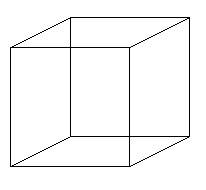
\includegraphics[scale=.7]{images/Necker_cube.png}
      \caption{The Necker Cube: insufficient sensory information to reach fixation on one explanatory model over another creates binocular rivalry between perceptual hypotheses}
        \label{fig:neckerCube}
   \end{center}
\end{figure}

It appears that human cognition has evolved a second order inferential mechanism that flexibly directs attention to certain sensory signals over others in order to successfully adjudicate between hypotheses for perceptual inputs \citep{Clark2013}.  In an inferential process likened to ``empirical Bayes,'' each error signal is conditioned with a precision weighting, which essentially functions to either ``dial-up'' or ``dial-down'' the volume on that signal's influence on the overall predictive model \citep{Clark2015}.  Precision weightings are proportional to the inverse variance of the model prior for each sensory input \citep{Ernst2004,FitzGerald2014}.  In other words, the volume of more reliable or more commonly encountered sensory inputs will be dialled-up; while the volume on less reliable or less commonly encountered sensory inputs will be dialled-down. This process of Bayesian precision weighting can be understood as the AIF's version of attention \citep{Ramstead2016}.

Precision weighting allows the brain to decide which prediction errors to pay attention to at which level of the coding hierarchy \citep[be it high and conceptual or deep and sensory][]{Friston2015}.  Iterative learning adjusts the precision weighting mechanism to strengthen prior probability distributions of models for future inference \citep{Robbins1964}.

Thus, not only does PC appear to be more computationally efficient, it also promises to be more flexible than alternative models of cognition---facilitated by a second-order mechanism of precision-weighting.  The process of prediction error minimisation accords neatly with the mandate of free energy minimisation prescribed by the AIF.  As I explain in more detail below, the PC paradigm provides a neurocomputational architecture capable of efficiently and flexibly integrating various sensory inputs (exteroceptive, interoceptive, and proprioceptive) into one overarching inferential process.


\myparagraph{Was it a thief or just the wind?\label{sect:windThief}}
To understand how the PC account applies to human cognition, consider the following example used by cognitive scientist Giovanni Pezzulo \textcite{Pezzulo2013}.  Imagine you wake up in the middle of the night to the sound of your bedroom window creaking.  At the higher levels of the predictive coding architecture, competing perceptual hypotheses emerge to explain the likely causes of the sensory experience.  For simplicity, assume that two plausible hypotheses emerge: 1) the wind outside caused the window to creak (wind), or 2) a thief is trying to break in to your house (thief).  The probability that the sensory experience of the window creaking is due to the wind can be represented by the equation in Figure ~\ref{fig:windThief}.  The predictive coding proposal is that the brain formulates a probability estimate based on:

\begin{enumerate}
  \item $P(wind)$: the model \textit{prior} formulated by previous experience (e.g., it has been windy at night recently, or in the case of $P(thief)$, there have been some recent thefts in the neighbourhood)
  \item $P(evidence|wind)$: the \textit{likelihood} that the sensory experience is caused by the wind (this value could be informed by other sources of information, e.g., the trees outside are also rustling, the dog is not barking (which may be the case if it were a thief, ($P(evidence|thief)$)
  \item Precision weighting: the reliability or certainty associated with your sensory inputs (it is dark in your room and so you may not trust your visual perception, you just woke up so could have been dreaming, etc.).  The precision weight is factored into the ``evidence.''
\end{enumerate}


\begin{figure}[htbp]
  \begin{center}
    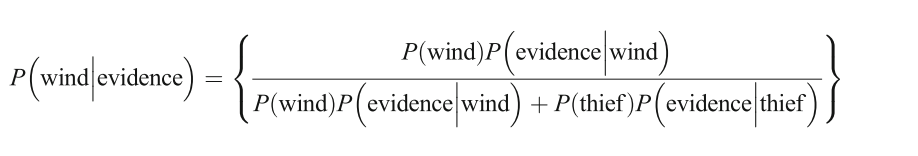
\includegraphics[scale=.5]{images/windThief.png}
      \caption{Bayesian model for the prediction of wind as the cause of the window creaking. Source: Pezzulo (2014)}
        \label{fig:windThief}
   \end{center}
\end{figure}

These two hypotheses (wind and thief) effectively compete on the basis of how well they explain the sensory stimuli.  The brain's capacity to quantify the uncertainty of any given sensory state (precision) facilitates optimal selection between competing predictions pertaining to the same bottom-up sensory signals.  In this example, based on the the priors ($P(wind) = .8$ (it has been windy recently) and $P(thief) = .2$ (no recent reports of theft)), and the (precision-weighted) evidence ($P(evidence|wind) = .6$ and $P(evidence|wind) = .5$ (roughly equivalent because it is dark and you have just woken up), the probability of wind ($= .8276$) is much higher than the probability of thief ($= .1724$).  In this case, the prediction that wind caused the window to creak wins out, and guides action and perception accordingly (you decide to go back to sleep).


\myparagraph{What makes the AIF ``active?''}
Original models of PC dealt primarily with ``exteroceptive'' information \citep[relating to stimuli that are external to an organism, i.e. visual, auditory, haptic perception][]{Rao1999,Friston2010}.  In the wind vs. thief model considered above, only exteroceptive evidence is considered, in the form of the auditory stimulus of the window creaking.  Research has since demonstrated that the PC approach can also account for ``proprioceptive'' information (relating to stimuli that are produced and perceived within an organism, especially those connected with the position and movement of the body), as well as ``interoceptive'' information  \citep[relating to stimuli produced within an organism, particularly by the body's organs (viscera) e.g., ``gut feelings,'' or elevated heart rate; see][]{Seth2013,FeldmanBarrett2015}.  Incorporating proprioceptive and interoceptive information sources into PC allows researchers to theoretically demonstrate that human cognition is both ``embodied''---inference is rooted in and contingent upon visceral, interoceptive information \citep[][]{Pezzulo2014}, as well as ``active'' \citep[in the sense that humans can move throughout the environment to reduce the discrepancy between proprioceptive predictions and actual body states, see][]{Friston2010,Clark2015}.

In the case of motor systems, agents are able to move their sensors in ways that amount to actively seeking or generating the sensory consequences that they (or rather, their predictive models) expect.  In this way, ``error signals self-suppress, not through neuronally mediated effects, but by eliciting movements that change bottom-up proprioceptive and sensory input'' \citep[][1349]{Friston2003}.  The hierarchical and nonlinear structure of predictive coding enables diverse sensory inputs feed into the same inferential mechanism.  Diverse functions of action, cognition and perception are thus integrated into an framework that is both embodied and enactive \citep{Friston2015}.  Embodied and active sources of information broaden the scope of human cognition beyond the brain and reduce reliance upon computationally intensive mental simulation as a driving force for action.  Instead, canny utilisation of extra-neural and bio-external affordances of the environment can support free energy minimisation \citep{Clark2015}.  Thus, the \textit{integrative} approach of the AIF allows for a conception of interlocking traditionally disparate sources of information---e.g., physical, emotional, and cognitive---into one inferential process.

Consider an ``active'' revision of the wind vs. thief example.  Two key differences in the model become apparent.  First, the evidence considered is broadened to include both interoceptive and proprioceptive information, in addition to exteroceptive evidence.  Assume that before you went to bed you just watched a horror movie, and when you woke up to the sound of a window creaking your heart began to pound and you immediately fixated on the hypothesis that a thief was causing your window to creak.  Fixation on the thief hypothesis can be explained by the contribution of interoceptive information (e.g., autonomic stress response, heart beat, etc.) to sensory the evidence \citep{Pezzulo2014}.  In addition, the incorporation of proprioceptive information into the model (for example, the possibility of moving to turn on the bed-side lamp) creates additional cognitive affordances through which higher level predictions could be strengthened (or free energy can be minimised).  This difference in the model demonstrates how perception, emotion, and action are functionally integrated in human cognition.

Second, broadening sensory inputs in the model also introduces the problem of differential reliability of sensory inputs.  The wind vs. thief example describes a situation in which exteroceptive information is relatively unreliable: it is dark, so visual inputs are restricted, and what you heard is unreliable because you just woke up and maybe it was part of a dream.  By contrast, interoceptive information is usually quite certain: you can be certain that your heart is pounding and that you feel unnerved.  In this particular case, interoceptive inputs may have a greater influence on the overall inference due to their reliability.  As explained above, evidence suggests that the brain deals with multiple sensory inputs via a process of ``Bayesian multisensory integration'' \citep{Ernst2004}, with the reliability of each sensory input proportional to the inverse of its variance.  In the wind vs. thief example, the interoceptive information from your body, precision-weighted as the most reliable source, will likely tip the model to favour the hypothesis that it is a thief, in which case you will move your body in ways that reconcile discrepancy between proprioceptive predictions that also correspond to the thief hypothesis, and therefore are tuned to a higher volume in the model. The result of this trajectory of action and perception may be that you act by turning on your bedside lamp \citep{Pezzulo2014}.

Thus, the combination of mutlisensory integration (of exteroceptive, proprioceptive, and interoceptive information) and Bayesian precision-weighting of prediction errors provides the necessary mechanics for a conception of human cognition that is both active and embodied.    In the following section, I introduce the concept of affordances as a necessary compliment to the PC paradigm and a core component of the AIF.

%Even if turning on the light would subsequently reveal that it was the wind all along,

%[; for a detailed discussion of the differences between traditional and active inference approaches to motor control, see Appendix ~\ref{app2:theory} Section  ~\ref{app2:motorControl}]  In the next section, I explain how active inference can be applied to joint action and shed light on the phenomenon of team click.



\subsubsection{Affordances}
In this section I introduce the concept of affordances as a necessary compliment to the generative models and its relevance to the AIF.  In brief, affordances can be understood within the AIF as extra-neural resources that couple with generative models to produce loops of action and perception \citep{Ramstead2016,Clark2015}.  The concept of affordance is crucial to facilitate an understanding how active inference unfolds in real-world settings.  While affordances have traditionally been studied narrowly as localised resources for basic perception \citep[e.g.][]{Fajen2011}, researchers working with the AIF have proposed an extension of the the concept of affordances to include a spectrum of objects, ranging from content-limited ``natural affordances,'' through to content-rich affordances mediated by cultural conventions and institutions \citep[cf.][]{Roepstorff2010,Ramstead2016}.

The theory of affordances, originally proposed by psychologist \textcite{Gibson1979} states that the world is perceived not only in terms of object shapes and spatial relationships, but also in terms of object possibilities for action.  This definition accords neatly with the propositions of the AIF, which posits Bayesian inference machines reliant on cognitive resources distributed throughout brains, bodies, and physical features of the task-specific environment in circular causal loops of perception and action.  Put simply, an affordance is the attribute of a hidden cause in the environment that induces (through PC architecture) predictions \citep[908]{Pezzulo2013}.  Repeated coupling between generative models and their extra-neural correlations in the environment give rise to dense causal relations between particular affordances and particular predictions.

Working within the AIF, \textcite[7]{Ramstead2016} propose that the extra-neural cognitive resources to which generative models couple (i.e., affordances) can be understood as a spectrum, with ``natural affordances'' at one end, and ``conventional affordances'' at the other \citep{Ramstead2016}.  Natural affordances pertain mainly to basic correlations between the organism and the environment that enable sensorimotor control and regulation: the physical features of the environment; the ground beneath our feet.  Conventional affordances, by contrast, often rely on consensus from other agents and culturally derived regularities; the carpet beneath our feet, or the keys at our fingertips, for example.  As Ramstead and colleagues explain:

\begin{quote}
  Successfully learned human conventions that govern action are also best conceptualised as affordances. Such affordances depend on shared sets of expectations, reflected in the ability to engage immersively in patterned cultural practices, which reference, depend on, or enact folk ontologies, moralities and epistemologies. We might call these ``conventional'' affordances.
\end{quote}

As \textcite[906]{Pezzulo2014} points out, PC hierarchies extend well beyond hypotheses concerning the source and reliability of immediate sensory inputs. At higher levels of the PC hierarchy, more profound regularities can be represented, such as long-term beliefs that are increasingly more removed from sensorimotor events. In humans, while higher order beliefs may be acquired mainly through cultural learning (rather than purely ``from the ground up'' via natural affordances),  these beliefs may still remain ``grounded'' through the linkage with lower-level sensory events).  Indeed, higher-order beliefs may need to remain grounded in sensory experience in order to retain long-term viability.

\textcite{Bruineberg2014} propose that affordances should be conceived of using a three-step topology. For any given agent, there exists a ``landscape'' of all possible affordances, within which an agent only engages with a specific ``field'' of affordances prescribed by the patterned coupling between predictive models and natural and cultural features of the environment; the affordances to which an individual brain is coupled at any one moment can be understood as ``solicitations.''  This three-level topology of affordances allows for a conception of the way in which repeated agent-environment coupling can give rise to particular regimes of attention, action, and perception within a vast landscape of all possible affordances.

When a specific field affordances or set of solicitations are conventional and shared, repeated coupling can generate regimes of \textit{shared} attention. For the purposes of this dissertation, conventional (cultural) affordances can thus be understood as regularities in the environment that cue multi-modal predictions for joint action.  This understanding incorporates factors that are traditionally understood to b psychologically explicit or ``external,'' such as societal values or similar cultural dimensions, \citep{Hofstede1991,Schwartz1992}, social practices and artefacts  \citep{Nisbett2003a}, as well as and ``internal,'' such as dominant modes of self-construal or dispositional and linguistic tendencies \citep{Markus1991}.  The concept of affordances enables an extension of the AIF beyond immediate sensorimotor processes, and into the domain traditionally understood as ``culture'' \citep{Roepstorff2010}.

In sum, the concept of affordances is an indispensable compliment to generative models of the AIF.  As discussed in the previous section (Section ~\ref{sect:predictiveCoding}, generative models can be understood as containing a spectrum of statistical complexity, ranging from basic (content-free) to elaborate (and seemingly content-rich) correlations.  The affordances to which these models couple (and therefore on which such models depend) can likewise be conceived of as existing on a spectrum, spanning natural and conventional (cultural) variants.  Importantly, the concept of affordances reveals the fact that higher-order generative models are contingent on couplings with higher-order affordances, i.e., culturally shared affordances.  In other words, higher cognitive processes are fundamentally social processes.   The correlation in complexity between generative models and their affordances provides a proximate explanatory mechanism for the observable fact that higher-order cognitive capacities for belief, reason, and language appear to be fundamentally contingent social and cultural processes, rather than purely innate capacities for which humans are naturally endowed \citep{Sperber1997,Henrich2015}.  The concept of affordances also offers an explanation for observable cross-cultural variation in action, perception, and attention \citep[cf.][]{Nisbett2003}.  Selective engagement with specific fields of affordances give rise to regimes of shared attention and beliefs that direct trajectories for individual and collective activity.


\myparagraph{Summary of the active inference approach to joint action}
To summarise, the AIF entails a radical inverse of traditional models of cognition that rely predominantly on bottom-up sensory inputs and top-down feature detection \citep[e.g.,][]{Marr1985}. Instead, active inference posits that top-down predictive models themselves shape perception and action, and the only information that travels forward (or from the ``bottom-up'') is the error signals that arise from discrepancies between predictions and the sensorium \citep{Pickering2014}.  AIF depicts a human cognitive system in which perception, mental simulation, emotion, and action are functionally and temporally integrated to manage uncertainty (free energy) inherent in interactions with the environment \citep{Clark2013}.  Importantly, these processes of generative modelling are dynamically coupled with affordances that span a spectrum of basal natural correlations with the physical features of the environment, through to elaborate culturally mediated beliefs and conventions.  The integrative approach of AIF allows for a theorisation of the interlocking physical, affective, and social dimensions of group exercise.


\section{Active inference applied to joint action \label{sect:activeInfJA}}
As explained above, traditional theoretical models of human cognition have struggled to integrate cognition with emotion, mental simulation with habitual response, flexibility with efficiency \citep{Clark2015}.
Team click is a powerful subjective experience in which many of these binaries appear to collapse and co-occur.  The AIF approach promises a testable theory of the embodied and dynamic dimensions of joint action.  In this section, I outline existing attempts to apply the AIF to joint action, and point to predictions relevant to team click and social bonding in joint action.
%, which appear to be maximised in team click.

%\myparagraph{Auxiliary approaches to joint action}
The AIF proposal offers a more integrative alternative to existing models of joint action, which rely on mechanisms of sensory prediction (of self, other, and joint actions) that are individually-bounded and auxiliary to joint action itself \citep{Pesquita2017}.   \textcite{Keller2016}, for example, presented a conceptual framework that applies an ``auxiliary forward model'' (AFM) approach to musical joint actions.  The AFM approach requires that agents produce predictive models responsible for individual action planning and control (self-internal models), prediction of others' actions (other-internal models), and representation of the shared goal (joint-internal models).  Of these three types of models, however, only self-internal models comprise the auxiliary predictive architecture (i.e., the forward model containing an efference copy of one's own action, and ``inverse models'' that are responsible for output of motor commands ~\ref{app2:theory}, Section ~\ref{app2:motorControl} for a more detailed explanation of these terms).  Thus, both anticipation and compensation in joint action depends on a control loop, whereby sensory information (error signals) are routed (fed-back) through self-internal models, which inform the production of auxiliary predictions---of self, other, and joint action---grounded in individual motor simulations.  Importantly, in this model,  error signals are fed-back only to the self-inverse model, as no inverse model for the joint action partner exists.

The longstanding proposal that individuals only produce auxiliary predictive models of their own actions (as opposed to others' actions too) has served to explain how individuals effectively attend to others in joint action.  With privileged access to an efferent copy of impending individual action, an agent is able to preemptively attenuate sensitivity to their own action, in order to attend to the actions (and prediction errors) of others \citep{Wolpert1998}.  For example, the AFM approach provides an explanation for the phenomenon of tickling, or specifically why it is near impossible to tickle oneself \citep[due to sensory attenuation resulting from the self-generated predictions about the consequences of action][]{Blakemore2003}. However, while the AFM has proven adequate to explain individual motor control, and some instances of joint action (such as tickling), it also contains potential shortcomings when applied to dynamical joint action scenarios.

\textcite{Pesquita2017} summarise three shortcomings when applying AFM to joint action.  First, the AFM model assumes a static and unchanging representation of the shared goal and the other's goal, and provides no mechanism through which the shared goal representation can be dynamically updated (based on prediction error signals).  This issue limits the ability of AFM to account for the real-world flexibility and interchangeability of shared goals (for example, the adaptive switching between the shared goal of carrying a table or the bench depending on the location of both objects).  Second, the same rigidity applies to other-inverse models.  The inability to directly and dynamically update other-models suggests the practical possibility that self and other models may gradually diverge over time due to the lack of sufficient predictive information regarding the actions of others \citep{Pickering2014}. Third, the AFM approach does not specify how sensory input is differentially used to update self and other models, which limits the model's ability to account for learning and adaptation within joint action \citep{Pesquita2017}.  Thus, not only does the AFM approach appear to be computationally intensive (due to the recruitment of auxiliary inverse models and dual motor commands, discussed in Section ~\ref{sect:predictiveCoding}), it also appears to be unable to fully account for the dynamic flexibility of real-world joint action.

\myparagraph{Generalised synchronisation as a dynamical foundation for joint action}
The AIF offers a thoroughly dynamical approach to joint action, whereby two (or more) Bayesian predictive brains committed to modelling each other in order to minimise free energy \citep{Friston2015,Friston2015a}. In order to achieve free energy minimisation, the sensory stimuli produced by co-actors in joint action must be pre-emptively modelled, just like other features of the sensorium (as explained above, see Section ~\ref{sect:thermoCog}).  This necessitates a scenario in which brain A has a model of brain B, which includes the fact brain B is modelling brain A, and so on---\textit{ad infinitum}.

The recurrent predictions of both brains about one another threatens an infinite runaway regress that could preclude accurate modelling of either brain.  However, as Friston and Frith demonstrate formally (mathematically), this recursion dissolves if the models of the two brains are formally similar \citep{Friston2015}.  When grounded in computational similarity, each brain is able to generate predictions of the sensory outcomes caused by itself and the other in the same way.  The authors propose that this will lead to dynamical ``generalised synchronisation'' \citep{Barreto2003}, or dynamical coupling between the internal models of both brains (for a more detailed explanation of general synchronisation and its dynamical underpinnings, see Appendix ~\ref{app2:theory} Section ~\ref{sect:generalSync}).  In this way, two or more brains are able to accurately predict each other's behaviour based on feedback of exteroceptive (sensory information from the actions of others and the task environment) and proprioceptive (pertaining one's own contribution to joint action) prediction errors.  In essence, other agents exist as affordances to which individual brains couple, and upon which individual brains become dependent for ongoing (joint) processes of action, perception, and attention.

In place of auxiliary processes of prediction, the AIF for joint action hinges instead on the function of precision weighting of prediction errors in order to facilitate and finesse joint action.  When performing action, the individual turns down the volume (reduce the precision weighting) on prediction errors relating to one's own action so that movement can occur unimpeded by over-attention to self-generated prediction errors \citep[an intuitive example of the opposite of this ideal scenario is when the flow of speech is interrupted due to the availability of exteroceptive auditory feedback in the case of a Skype call][]{Friston2015}.  Alternatively, when attending the the action of others, the attenuation of proprioceptive error signals can cease. In this way, precision weighting is used to flexibly adjust the volume of multi-modal prediction errors (exteroceptive, interoceptive, and proprioceptive) in order to finesse and sustain generalised synchronisation (the shared narrative on which joint action is sustained).

Heuristically, this suggests that active inference in joint action takes one of two modes; either 1) flexibly attending to sensations or
2) acting during periods of sensory attenuation \citep{Friston2015}.  The active inference explanation for ticklishness, for example, is an inferential mode in which the volume on proprioceptive prediction error is ``dialled-up.''  The failure of self-tickling, by contrast, pertains to a mode of active inference in which the volume of proprioceptive prediction is ``dialled-down'' to enable smooth flow of action execution.
  \footnote{Recall also that instances of tickling commonly involve a stationary victim. While it indeed appears almost impossible to tickle oneself, it is also rare to be tickled while moving, i.e., acting during periods of sensory attenuation.}


\myparagraph{Predictive Joint Action Model (PJAM)\label{sect:PJAM}}
\textcite{Pesquita2017} have formulated a minimal architecture for an active inference approach to joint action, which they term a ``Predictive Joint Action Model'' (PJAM).  PJAM is comprised of three hierarchical levels of inference: goal representation, action-planning, and sensory routing (see figure ~\ref{fig:PJAM}).  Each level of the hierarchical model is informed by prediction errors from the level below, and the model works iteratively to minimise free energy in joint action scenarios.  In line with the AIF, PJAM does away with auxiliary processes of motor control and efferent copies, and posits instead that joint action emerges directly from two or more individuals reaching generalised synchronisation by converging on equivalent predictive models for joint action \citep{Friston2015}.

  \begin{figure}[htbp]
    \begin{center}
      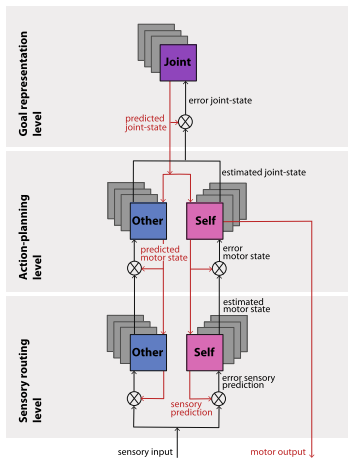
\includegraphics[scale=.8]{images/PJAM.png}
        \caption{The Predictive Joint Action Model \citep{Pesquita2017}}
          \label{fig:PJAM}
     \end{center}
  \end{figure}

In contrast to the AFM approach, which posits a shared goal representation deriving from self-internal models, the PJAM suggests that a shared goal derives primarily from the dynamical coupling of agents to each other and to other (shared) affordances of the task-specific environment.  Thus, rather than being wholly explicit, propositional, or pre-set, the shared goal is understood to span the entire predictive hierarchy, with basal coupling of sensorimotor processes at the lower end, through to more elaborate models that facilitate more explicit or propositional content, at the higher end.  In a bidirectional cascade of prediction and prediction error, the ``shared narrative'' at the goal representation level generates discrete action plans for self and other, which are then tested against prediction errors arising from the sensory routing models below \citep{Pesquita2017}.


\subsubsection{Evidence in support of PJAM}
PJAM (and the AIF which it extends) predicts that joint action will be established and maintained through generalised synchronisation between two or more predictive brains driven by an overarching mandate of free energy minimisation \citep{Friston2015}.  In particular, PJAM predicts that co-actors in joint action will generate predictive models that reflect 1) a shared goal, 2) action plans for self and other, and 3) routing instructions for sensory inputs.  Consistent with the modelling view of the AIF (see Section ~\ref{sect:thermoCog}), these three layers of generative models will reflect an hierarchy of complexity, and will be coupled to a continuum of natural and conventional affordances.  Below I outline existing experimental evidence in support of these predictions.

\myparagraph{Evidence for generalised synchronisation in joint action}
Evidence that musicians maintain shared representation of desired unified sound of an ensemble \citep{Keller2008}, track deviations from desired joint state \citep{Loehr2013}, and allow shared goal predictions to guide future action \citep{Loehr2016}, confirms the hypothesis that co-actors share a dynamical and flexible shared goal---a shared narrative or common ground.  PJAM specifically predicts that the foundation for this shared narrative will be dynamical, i.e., it will involve coupling of system component degrees of freedom of co-actors in joint action \citep{Turvey1978,Schmidt1990}. Dynamic coupling can be identified by two core properties:  1) dimensional compression (potentially independent DF are coupled so that the synergy possesses a lower dimensionality than the set of components from which it arises) and 2) reciprocal compensation \citep[the ability of one component of a synergy to react to changes in others][]{Riley2011}.

An accumulation of evidence on multiple levels of human behaviour, from brain function \citep{Yufik1998,Sengupta2013}, to interpersonal interactions \citep{Kelso2009,Riley2011,Fusaroli2014}, to large-scale human societal dynamics \citep{Nowak2017} supports the existence of dynamic coupling.  In the case of joint action in particular, individuals have been found to couple and reciprocally constrain their movements reducing the overall control needed to maintain effective cooperation \citep{Ramenzoni2011,Ramenzoni2012,Riley2011,Schmidt1990}.  Studies of real-world joint action scenarios such as dancing, martial arts, and moving objects like furniture have revealed evidence for dynamic coupling between co-actors.  In these studies, specific component degrees of freedom are modelled as coupled oscillators \citep[using the HKB model, which describes the change in the relative phase between two oscillatory components. See][]{Haken1985,Kelso1986}.  Interestingly, dynamic coupling of movement has been measured beyond dyadic synchronisation, in the analysis of sub-phases of team sports \citep{Passos2014,Duarte2012} and group dancing \citep{Chauvigne2017}.  For a more thorough explanation of dynamic coupling in human movement systems, including methods for measuring dynamical quantities, see Appendix ~\ref{app2:theory} Section ~\ref{app2:dynamicCoupling}.

This evidence is supported by recent research focussed on the movement signatures of joint action that resemble instances of ``identical synchronisation,'' or the idea of being ``in the zone'' with a co-actor. Working within the common dyadic ``mirror game'' paradigm, \textcite{Noy2011,Noy2015,Hart2014} have identified ``co-confident motion'' (CC motion) as a canonical movement pattern of synchronised motion characterised by smooth and jitter-less motion, without the typical jitter resulting from reactive control in more commonly encountered leader-follower patterns.  In CC motion, different players appear to shift their basic motion signatures to a movement shape that is altogether different from their individually preferred shapes \citep{Hart2014}. Importantly, the pattern of CC motion shares the same sine wave shape as the optimal solution of the minimum jerk model, a well-known motor control model for rhythmic motion \citep{Hogan2007}.  This evidence accords with the proposal that joint action is underwritten by a ``shared narrative'' that transcends individual action tendencies of self and other and produces a  ``we-mode'' of social cognition (exemplified by CC motion) \citep{Gallotti2013}.

\myparagraph{Evidence for self and other action plans}
On the level of self and other action plans, experimental evidence suggests that co-actors generate internal models of self and other either spontaneously and involuntarily---as in the commonly used social simon task experimental paradigm \citep{Sebanz2003,Atmaca2008}---or more deliberately---as in a coordinated dyadic horizontal jumping task \citep{Vesper2012}.  \textcite{Loehr2016} demonstrate that when learning a joint piano piece, musicians are able to better perform a piece together rather than solo, which suggests that representations about each participant in joint action are encoded within the joint context of the interaction.  Studies also show that the capacity for co-representation of self and other action plans is modulated by mood \citep[positive or negative affect, see][]{Kuhbandner2010}, self-concept and social orientation \citep{Colzato2012,Colzato2012a}, and processes of group membership \citep{DeBruijn2008,Iani2013}. This evidence lends support to the proposal that active inference involves coupling with various natural and conventional affordances in order to flexibly integrate information deriving form various sensory inputs.

The evidence outline immediately above is supported by parallel strands of research in psychology \citep{Prinz1990,Prinz1997,Prinz2013}, neurophysiology \citep{Rizzolatti2004,Rizzolatti2010}, and neurocognition \citep{Wolpert1998,Wolpert2000} that interpersonal behavioural coordination in joint action is facilitated by the intrinsic links between action perception and action execution in the human brain.  In essence, action-perception coupling refers to the ostensive co-occurrence of a stimulus for action and its motor representation.  For example, for individuals who have mastered a certain sensorimotor task, the representation of a perceptual effect (say the sound of a middle-C on a piano) can trigger the movement necessary to produce the effect itself (motor instructions for playing the middle-C key on a piano) \citep{Novembre2014}. Evidence suggests that skilled individuals not only develop generative models for self action, but also for the actions of others in joint action \citep{Novembre2012}. Action-perception links can be used for monitoring and integrating (e.g., timing or combined pitches) the actions of other ensemble members with self-generated actions \citep{Loehr2013}, and these effects appear to be stronger in individuals with high perspective taking skills \citep{Novembre2012,Loehr2013}.  The overlap between mechanisms for action production and action observation suggests that individuals may represent their own and others’ actions in a commensurable format.  Training-induced motoric representation of self and other actions may facilitate various capacities important for joint action, such as prediction, adaptation, and entrainment (for a more detailed treatment of action-perception links and their relevance to joint action, see Appendix ~\ref{app2:theory} Section ~\ref{app2:actionPerceptionLinks}).

\myparagraph{Evidence for sensory routing}
On a sensory-routing level, evidence suggests that modulation in sensory attenuation is driven by the predictability of the outcome, as opposed to necessarily being driven by the presence or absence of auxilliary efference copies \citep{Sato2008}.  In addition, attributing sensory consequences to joint action partners is linked to cooperative success \citep{Chaminade2012}, suggesting that finely tuned sensory routing based on predictions of self and other actions could be key to successful coordination.

In sum, PJAM provides a framework for the function of active inference in joint action.  PJAM proposes a dynamical model of joint action, whereby the predictive models of two or more brains are coupled to produce a common ground upon which free energy minimisation can occur.  In the section below, I outline how this process of general synchronisation could explain the phenomenon of team click, as well as the achievement of social connection through joint action.



\subsubsection{AIF for team click and social bonding in joint action\label{}}

How can the AIF be used to account for team click and social bonding in joint action? In this section, I draw attention to evidence for mechanisms relevant to joint action that could generate

As explained in Chapter ~\ref{chap:intro}, the link between joint action and social bonding has been addressed in the behavioural mimicry and synchrony literatures \citep[see Chapter ~\ref{chap:intro} Section ~\ref{sect:synchrony}. There is now strong evidence to suggest that a combination of 1) neuropharmacological reward arising from lower-cognitive affective mechanisms, 2) self-other merging resulting from neurocognitive alignment, and 3) reinforcement of cooperative relationships owing to experience of interpersonal association in joint action generates a psychophysiological environment conducive to generating social bonds.  Yet, almost all of these studies operationalise joint action as exact in-phase behavioural synchrony \citep[see][]{Mogan2017}, and there is much less substantive evidence of the bonding effects of complex and dynamic joint action scenarios \citep[but see][]{Marsh2009,Miles2009,Lumsden2012}.  More fundamentally, the research dedicated to the putative synchrony-bonding link focusses most of its attention on the proximate and affective mechanisms of joint action, and accounts less for how synchrony-induced lower-level physiological and affective mechanisms facilitate more elaborate (higher-order) cognitive and social processes that also form part of processes of bondedness, social cohesion, and cultural transmission \citep{Heyes2012}.

As I argue in this dissertation, these dual shortcomings of the social cognition of joint action represent two sides of the same coin. On one side, how behaviourally complex joint actions generate social and physiological effects remains poorly theorised; on the other side, the causal role of physiological and social effects on complex cognitive and cultural processes (i.e., cultural transmission and evolution) is also poorly understood.  I suggest that adopting an integrative model of cognition (AIF) can help advance understandings of the interlocking physical, affective, cognitive, and cultural mechanisms of social connection in joint action and cognitive and evolutionary processes more generally \citep{Ramstead2018}. Indeed, the AIF serves to collapse the traditional distinction between physical, affective, cognitive, and cultural processes, under one overarching mandate of free energy minimisation.

\myparagraph{Team click}

As discussed above, the AIF for joint action suggests that successful performance in joint action will require a continuum of generative models tightly coupled to a spectrum of natural and conventional affordances \citep{Clark2015}.  In other words, a range of basic  The cognitive mechanisms that generate subjective perceptions of multimodal alignment between co-actors---what I term team click---could explain the relationship between joint action and social bonding in group exercise.

Recap click components and reduce to dimensions (surprise, viscerality, agency); how these dimensions track to mechanisms of AIF (multisensory integration

%\myparagraph{The social quirks arising from 2nd-order bayesian inference}




\myparagraph{Surprise}
Surprise (unanticipated error: less precision, higher reward)
Friston,
Chetverikov2016


\myparagraph{Visceral}
(due to inherent cognitive challenge of JA)

Could be due to

\myparagraph{Agency}

Sensory tuning and agency: blurring boundaries between self and other agency



% Please add the following required packages to your document preamble:
% \usepackage{booktabs}
% \usepackage[normalem]{ulem}
% \useunder{\uline}{\ul}{}

\newpage
\newgeometry{margin=0.5cm} % modify this if you need even more space
\begin{landscape}

\begin{table}[]
\begin{tabular}{@{}lllll@{}}
\toprule
\textbf{Component}                                                        & \textbf{Dimension} & \textbf{AIF mechanism}                                                                                        & \textbf{Predicted function}                                                                                                                                                                                                                                                                                                                                                                                                                & \textbf{Predictions for joint action}                                                                                                                                                                                                                                      \\ \midrule
Surprise                                                                  & \textbf{Affective} & \begin{tabular}[c]{@{}l@{}}Precision-weighting \\ (exploitation exploration, \\ cf. Friston2013)\end{tabular} & \begin{tabular}[c]{@{}l@{}}Attention will be allocated to sensory inputs\\  as a function of their prior probability\\ distribution; Affect (surprise) will\\  be allocated to predictions as function of inverse \\ prior probability; i.e., higher probability predictions \\ receive more attention but lower reward; lower probability predictions \\ but receive less attention but higher \\ reward (Chetkerov, Fiston)\end{tabular} & \begin{tabular}[c]{@{}l@{}}Inherent uncertainty of real-world joint action \\ (the df problem, cf. Bernstein 1967), makes successful coordination improbable, but highly rewarding:\end{tabular}                                                                           \\
                                                                          &                    &                                                                                                               &                                                                                                                                                                                                                                                                                                                                                                                                                                            &                                                                                                                                                                                                                                                                            \\
Group flow                                                                & \textbf{Visceral}  & \begin{tabular}[c]{@{}l@{}}Multimodal sensory integration \\ (Pezzulo 2014)\end{tabular}                      & \begin{tabular}[c]{@{}l@{}}More reliable sensory inputs will receive greater \\ precision-weighting\end{tabular}                                                                                                                                                                                                                                                                                                                           & \begin{tabular}[c]{@{}l@{}}Unreliability of exteroceptive predictions in joint \\ action will generate a decrease precision \\ on exteroceptive predictions, and increase precision of\\ interoceptive predictions (Pezzulo2014,\\ Seth2013, Feldman Barrett)\end{tabular} \\
                                                                          &                    &                                                                                                               &                                                                                                                                                                                                                                                                                                                                                                                                                                            &                                                                                                                                                                                                                                                                            \\
Tacit understanding                                                       &                    &                                                                                                               &                                                                                                                                                                                                                                                                                                                                                                                                                                            &                                                                                                                                                                                                                                                                            \\
                                                                          &                    &                                                                                                               &                                                                                                                                                                                                                                                                                                                                                                                                                                            &                                                                                                                                                                                                                                                                            \\
Atmosphere or aura                                                        &                    &                                                                                                               &                                                                                                                                                                                                                                                                                                                                                                                                                                            &                                                                                                                                                                                                                                                                            \\
                                                                          &                    &                                                                                                               &                                                                                                                                                                                                                                                                                                                                                                                                                                            &                                                                                                                                                                                                                                                                            \\
\begin{tabular}[c]{@{}l@{}}Blurred self and other \\ agency\end{tabular}  & \textbf{Agentic}   & Sensory attenuation                                                                                           &                                                                                                                                                                                                                                                                                                                                                                                                                                            &                                                                                                                                                                                                                                                                            \\
\textit{}                                                                 &                    & Precision-weighting                                                                                           &                                                                                                                                                                                                                                                                                                                                                                                                                                            &                                                                                                                                                                                                                                                                            \\
\begin{tabular}[c]{@{}l@{}}Ability extended \\ by others\end{tabular}     &                    &                                                                                                               &                                                                                                                                                                                                                                                                                                                                                                                                                                            &                                                                                                                                                                                                                                                                            \\
\textit{}                                                                 &                    &                                                                                                               &                                                                                                                                                                                                                                                                                                                                                                                                                                            &                                                                                                                                                                                                                                                                            \\
\begin{tabular}[c]{@{}l@{}}Reliability of self \\ and others\end{tabular} &                    &                                                                                                               &                                                                                                                                                                                                                                                                                                                                                                                                                                            &                                                                                                                                                                                                                                                                            \\
                                                                          &                    &                                                                                                               &                                                                                                                                                                                                                                                                                                                                                                                                                                            &                                                                                                                                                                                                                                                                            \\ \bottomrule
\end{tabular}
\caption{Dimensions of team click and their relevant mechanisms as predicted by the AIF.}
\label{tab:teamClickMechanismsAIF}
\end{table}

\end{landscape}
\restoregeometry






\myparagraph{Social bonding}


Shared narrative:


Higher-order social identification

dense coupling of entire hierarchy of models with affordances in dense coupling (to minimise free energy).

SHW: while he was able to reproduce the explicit content of group membership in interview, he lacked conviction, he lacked a personal grasp.  When he game back in to my room, he had embodied (internalised)
the content, and as such it was completely transformative of his capacity to engage, relate, and interact.





The radical proposal of the AIF for joint action is that, unlike the AFM approach, the AIF formally theorises the way in which cognitive resources are shared between two or more brains, bodies, and the task-specific environment \citep{Clark2015}.  Therefore, social connection in joint action can be conceived as dynamic coupling between agents, which spans a continuum of basal sensorimotor processes, through to higher order beliefs facilitated by regimes of shared attention.  In this sense, social connection in joint action could arise in situations in which individuals perceive click between co-actors and other affordances contained within a certain field of activity.  In this dissertation, I develop the idea that in real world joint action scenarios such as interaction team sport, co-actors interact and rehearse their behaviours to produce a hierarchy of aligned representations, an implicit ``common ground'' \citep[cf.][]{Noy2017} on which joint action can unfold, and social connection may be found through team click.

%we are already connected!! (China, fusion)
%This ``shared narrative'' which supposedly transcends agency, is supported by the self-organising
























\section{Active inference in group exercise \label{sect:activeInfGE}}

In the previous section I reviewed evidence in support the AIF for joint action, and possible pathways between joint action, team click, and social bonding.  The AIF begins with the assumption that, on a basal level, joint action consists of two or more Bayesian inferential systems attempting to minimise free energy by modelling the hidden causes of sensory stimuli.  From sheer computational perspective, joint action is an inherently challenging task, but it appears that ``general synchronisation'' derived from the coupling of two or more agents facilitates a shared narrative (functionally equivalent models for joint action).  This perceptual common ground resembles a situation in which ``adjustments for ``Am I?'' and ``Are You?'' and ``Where Are We?'' and stuff like that...'' (see Section ~\ref{sect:teamClickIntro}) dissolve, and a transcendent ``we-mode'' of collective agency is glimpsed \citep[][]{Friston2015}.  Anecdote and observation of real-world joint action scenarios suggests that achieving the ``click'' of joint action---in spite of its uncertainty, and however momentarily it lasts---can be a deeply rewarding experience.  In the case of joint action in group exercise contexts, it appears that various features of group exercise serve to amplify both the challenges of joint action, as well as the psycho-social rewards derivable from adherence.

\myparagraph{Group exercise involves multi-agent (and not just dyadic) joint action}
Above and beyond normal day-to-day instances of communication and exchange, joint action in group exercise contexts such as sport place extreme cognitive load on participants. The active inference approach to joint action outlined above is based on preliminary models of dyadic joint action involving turn taking \citep[i.e., in bird song exchanges][]{Friston2015}.  Group exercise contexts, particularly modern sport contexts, often involve large numbers of co-participants, in either ``inter-active'' or ``co-active'' modes of coordination.
    \footnote{
    In co-active sports (e.g., bowling, archery), team members perform separately and the team outcome is a product of combined individual performances. In interactive sports (e.g., volleyball, soccer, rugby), goal accomplishment requires the establishment of complex patterns of interaction and coordination among team members \citep{Filho2014}.
    }
Thus, achieving cognitive synchronisation in joint action of group exercise contexts may be much more difficult.  Evolutionary Anthropologist Robin Dunbar \textcite{Dunbar1992} proposes that the ratio of human neocortex size to total brain volume imposes an upper cognitive limit on real-time coordination of behaviour of approximately four to five individuals.  The sheer computational burden of modelling multiple agents in group exercise may place an unmanageable cognitive load on our normal healthy processes of active inference.  Indeed, at the very least, multi-agent joint action poses a challenge for the existing theoretical model for joint action (PJAM), which is formulated primarily based on dyadic interactions \citep{Pesquita2017}.

\myparagraph{Joint action in group exercise is ``on-line'' and ``in-the-moment''}
Particularly in the case of interactive team sports, interpersonal movement coordination is often executed ``on-line'' and ``in the moment,'' as opposed to step-by-step turn taking.  This fact poses a challenge to Friston and Frith's proposal that active inference in joint action comprises two modes (either actively attending to sensory stimuli, or else moving while in a state of sensory attenuation, see Section ~\ref{sect:activeInfJA} above).  Exactly what occurs when actors need to concurrently move and sense others moving at the same is poorly understood.  What happens to the precision weightings---the volume gauges---on proprioceptive, interoceptive, and exteroceptive prediction errors In instances of dynamic interactive joint action involving co-occurence of movement between agents in joint action?   What is the impact of on-line and in the moment join action on the experiences of agency in group exercise?  Empirical research is yet to provide answers to these questions.

\myparagraph{Group exercise involves competition}
As if the cognitive load of multiple agents and on-line coordination of complex schemas for joint action was not enough for the humble human brain, interactional team sports also usually involves \textit{competition}.  While competition in sport is usually adorned with elaborate social meanings surrounding the ethics of winning and losing \citep{McNamee2008}, on a cognitive level, competition in joint action entails one individual or team of individuals actively attempting to foil or disrupt the predictive models of another individual or team of individuals \citep{Reimer2006}.  The competitive dimension of interactional team sports thus serves to further spike cognitive uncertainty between co-actors in joint action.  The uncertainty involved in competitive joint action scenarios could have further implications for the ability of second-order Bayesian inference concerning the reliability of sensory inputs \citep{Pezzulo2014}.

\myparagraph{Group exercise involves metabolic tradeoffs in the brain}
In addition to these heightened cognitive challenges associated with complex and dynamic joint action in group exercise, high levels of physiological exertion characteristic of group exercise could also serve to spike uncertainty.  Neuroscientist Arne Dietrich draws attention to the fact that physical exercise is at its core a stressor that places extreme energy demands the organism \citep{Dietrich2011}.
Such a situation will necessitate an energy tradeoff in the brain, whereby energetically costly brain regions inessential to movement execution are temporarily downregulated \citep{Dietrich2004b}.  Dietrich suggests that experiences of flow and the ``runner's high'' in exercise could be the result of temporary downregulation of energetically costly brain regions inessential to movement execution  \citep{Dietrich2004b}.  Dietrich and colleagues propose candidate areas of the dorsolateral prefrontal cortex responsible for self-monitoring and proprioceptive sensory attenuation \citep[commonly known as the ``inner critic'' regions of the brain, see][]{Limb2008}.  It is currently not well understood precisely whether or how neurometabolic tradeoffs in the brain could impact upon joint action and the experience of team click.  However, it is conceivable that metabolic tradeoffs in the brain owing to prolonged physiological stress may have implications for the second-order inferential processes of precision weighting sensory inputs.


\subsection{Free energy minimisation in group exercise demands greater reliance on extra-neural affordances \label{sect:extraNeural}}
To summarise, the combination of cognitive demands associated with tracking and modelling multiple agents ``in-the-moment,'' the neurometabolic tradeoffs associated with (often extreme) levels of physiological exertion, and even the competitive dimension of some group exercise contexts (for example interactive team sports), could create an environment in which humans' usual cognitive capacities are strained and compromised.  The fact that experiences of team click are particularly prevalent in group exercise contexts (compared to more mundane or quotidian instances of joint action) suggests that amplification of uncertainty and stress in group exercise could be a critical factor in facilitating powerful psychosocial effects.

The active inference approach would predict that individuals, when faced with the extreme cognitive uncertainty of joint action in group exercise, will tend to preference mechanisms that maximise uncertainty reduction (minimise uncertainty).  In the case of joint action in group exercise, this may entail reliance on predictive models that outsource the computational cost to affordances beyond the brain, or at least the metabolically expensive cortical areas of the brain \citep{Dietrich2004,Clark2015}.  In the case of highly skilled practitioners, whose predictive models for action have been finely tuned to the affordances of the task environment (inlcuding co-actors), it is plausible that extra-neural and even extra-personal resources (e.g., physical features of the task environment) could provide a more cognitively efficient and effective route to the performance of successful joint action and thus the minimisation of free energy.

Various strands of evidence support these predictions.  Studies of highly skilled practitioners in joint action demonstrate that more technically competent practitioners generate more accurate predictive models for joint action than less technically competent practitioners \citep{Tomeo2012,Aglioti2008,Mulligan2016}.   In studies involving skilled versus non-skilled practitioners in dyadic interactions, it has been shown that more skilled practitioners create stronger dynamical coupling through flexibly modulating their actions with others \citep{Schmidt2011,Caron2017}. These findings are corroborated by other studies that find that professional footballers (versus novice controls) are able to more accurately predict the direction of a kick from another player's body kinematics (\cite{Tomeo2012}, see also \cite{Aglioti2008,Mulligan2016} for similar results with basketball and dart players).  When analysing co-regulation between members of basketball teams, \textcite{Bourbousson2015} showed that more expert teams made fewer mutual adjustments (at the level of the activity that was meaningful for co-actors), suggesting an enhanced capability of expert social systems to achieve and maintain an optimal level of awareness during the unfolding activity.

A recent field study with expert rowers revealed that athletes predominantly utilised
extra-personal (rather than inter-personal) regulation processes in order to facilitate and sustain joint action, and attention to interpersonal regulation occurred only during instances of expectation violation concerning performance in joint action \citep[; for a full explanation of this study, see Appendix ~\ref{app2:theory} Section ~\ref{sect:rowerStudy}]{RKiouak2016}. These results suggest that athletes used the affordances of the environment to mediate the arrangement of individual and joint activities \citep{Bourbousson2011,Bourbousson2012}.  Taken together, this evidence supports the prediction for a tendency for co-actors in joint action to utilise neurocomputationally conservative models and coupling with extra-neural affordances under circumstances of high levels of free energy (such as those common to group exercise).


\subsection{Team click and the dark room dilemma}
The evidence reviewed above demonstrates the human ability to flexibly deploy a range of cognitive strategies, seemingly towards the ultimate goal of free energy minimisation.  Inherent in the application of the free energy principle to group exercise is the paradox that group exercise is an activity that appears to deliberately amplify uncertainty.  In the active inference proposal outlined above, humans are depicted as free-energy minimising systems, driven by the ultimate goal of reducing surprise and maximising efficiency in their interactions with the environment \citep{Friston2010}.  Why do humans seek out and receive high rewards through activity in environments riddled with uncertainty?

On the face of things, the free energy mandate suggests an ``ultimate stable state'' \citep{Mumford1992}, in which all surprise minimised.  As evocatively described by Mumford:

\begin{quote}
  How can a neural imperative to minimize prediction error by enslaving perception, action, and attention accommodate the obvious fact that animals don’t simply seek a nice dark room and stay in it? Surely staying still inside a darkened room would afford easy and nigh-perfect prediction of our own unfolding neural states? Doesn’t the story thus leave out much that really matters for adaptive success: things like boredom, curiosity, play, exploration, foraging, and the thrill of the hunt? \citep[243]{Mumford1992}
\end{quote}

The simple response is that animals (humans included) live and forage in a changing and challenging world, and hence ``expect'' to deploy quite complex strategies to stay within our species-specific window of viability \citep{Bruineberg2014}.  As Clark explains,

\begin{quote}
  Change, motion, exploration, and search are themselves valuable for organisms living in worlds where resources are unevenly spread and new threats and opportunities continuously arise.  This means that change, motion, exploration, and search themselves become predicted and enacted accordingly \citep[193]{Clark2013}
\end{quote}


Agents infer a policy that minimises surprise by minimising the difference (or relative entropy) between likely and desired outcomes, which involves both pursuing the goal-state that has the highest expected utility (often termed “exploitation”) and visiting a number of different goal-states (“exploration”). Crucially, the opportunity to visit new states increases the value of the current state. Casting decision-making problems within a variational framework, therefore, predicts that our behavior is governed by both the entropy and expected utility of future states. This dissolves any dialectic between minimizing surprise and exploration or novelty seeking.
(Schwartenbeck2013)

There is evidence to suggest that the tradeoff between free energy minimisation and the search for novelty, creativity, and play (i.e., uncertainty) appears to be supported by a regime of affective rewards calibrated to precision-weighting dynamics \citep{Chetverikov2016}.
The details of these proximate mechanisms could shed light on the phenomenon of team click and its associated downstream psychosocial effects, including social bonding and social cohesion.  Joint action in group exercise, and the phenomenon of team click in particular thus offers a fascinating space in which to investigate the social cognition of active inference in joint action.  Active inference provides a theoretical frame through which the social cognition of joint action can be more clearly rendered and comprehended.

%How, then, do we explain the widespread prevalence of group exercise contexts, which appear to be riddled with uncertainty owing to the overwhelming complexity of joint action requirements and extreme physiological demands?  The phenomenon of team click could lie at the heart of an explanation to this paradox.

\subsection{AIF for team click and social bonding in group exercise}


\myparagraph{joint action to team click}
Preference for visceral evidence (most reliable)

Strain on precision weighting --> self-other blurring

Higher surprise



\myparagraph{team click to social bonding}


Higher interdependence: greater reliance on both visceral and narrative


































\section{A novel theory of social bonding through joint action\label{sect:novelTheory}}

As explained above, the explanatory power of PJAM in particular (the AIF more generally) lies in its capacity to incorporate various cognitive strategies within one overarching mandate of free energy minimisation \citep{Clark2015}.  The distinction between cortical and extra-cortical, mental and emotional, model-based and model-free cognitive processes dissolves, and in place of these dualisms, a continuum of cognitive strategies are flexibly deployed to exploit brain, body, and bio-external resources \citep{Pezzulo2013}.  Bayesian optimisation facilitates flexibility: the volume on sensory prediction error signals is either ``dialled-up'' or ``dialled-down,'' depending on their reliability judged by prior experience (inverse of variance of the prior distribution). Thus, just as the binary distinction between mental and emotional collapses, so too does the distinction between external and internal, exteroceptive and interoceptive \citep[and proprioceptive][]{Seth2013}.

This conception of joint action allows for a full consideration of the interlocking physical, cognitive, and social processes outlined in in Chapter ~\ref{chap:intro}.   Anecdotal and observational evidence suggests that team click is at once mental and embodied, cognitive as well as emotional, metaphysical (i.e., mysterious) as well as deeply grounded in visceral sensations (see Chapter ~\ref{chap:intro} Section ~\ref{sect:adrian}).

Joint action in group exercise creates a unique environment for social cognition, defined by extreme levels of cognitive uncertainty.  Group exercise involves high cognitive load associated with complex joint action requirements involving many actors, many hierarchical layers of joint goals over various sensory modalities and spatiotemporal scales. The ``in the moment'' execution demands also constrain cognitive processing, and encourage a reliance on cognitive resources located in extra-neural and bio-external domains \citep{Bourbousson2016}.  In addition, strenuous physical exercise could also entail neurocognitive tradeoffs that further strain individual ability to reduce free energy in joint action \citep{Dietrich2004b}.


Evidence discussed above suggests that optimal solutions to joint action typical of group exercise may tend to favour the recruitment of more extra-neural resources as a way of minimising free energy, whereas less efficient solutions to joint action may rely on more computationally intensive procedures in order to reduce free energy (see Section ~\ref{sect:extraNeural}).  The social cognition of these processes in joint action have not yet been closely considered \citep[but see ][]{Marsh2009,Lumsden2012}.


In the sections that follow, I propose a novel theory of social bonding through joint action, mediated by the phenomenon of team click. I do so by first explaining how joint action typical of group exercise can generate team click, and second how team click can lead to social bonding.

\subsection{Perceptions of success in joint action predict team click\label{sect:JASuccessTeamClick}}

The components of team click outlined above indicate that this often observed phenomenon contains elements of positive expectation violation or surprise, deriving from an experience of tacit or implicit coordination in joint action.  The phenomenology of team click can also involve the blurring of boundaries between self and others in the team, the perception of atmosphere or aura surrounding the group, as well as a perception of reliability of teammates and the self to successfully perform joint action.

How does joint action in group exercise generate the experience of team click?

\subsubsection{Dialled-up interoception}
Given these conditions, an active inference approach would predict the following.  First, a Bayesian brain tasked with weighting precision errors in highly uncertain, on-line joint action would likely turn down the volume on exteroceptive precision errors.  Think back to the wind vs thief example used above (Section ~\ref{sect:windThief}). In some respects, waking up in a dark room in the middle of the night is not too dissimilar to taking the rugby field: the reliability of exteroceptive information will be less reliable than information generated internally, via interoceptive and proprioceptive inputs. As such, it could be predicted that the interoceptive and proprioceptive inputs to the total evidence will be weighted more reliable than exteroceptive inputs.

Second, consider that group exercise requires constant execution of movement, contemporaneous with the movement of others. As discussed above, movement requires the attenuation of proprioceptive information (so as not to interrupt the flow of movement itself).  Thus, it can be predicted that the volume on proprioceptive error signals will at times be turned down low, at least while participants are executing movement.  There may need to be some optimal tradeoff here, in which the volume is not turned down too low, so as to keep track of the movements of others while moving.

In this situation, with the volume on exteroceptive information turned down, and proprioceptive inputs attenuated to allow for movement, it can be seen that interoceptive inputs could enjoy the most precision of all available sensory sources. This situation could conceivably explain the tacit ``feel'' of team click.  Interoceptive information could therefore provide an embodied grounding for the feeling of click.  This would make sense considering that often athlete descriptions of flow and team click involve pre-linguistic and pre-perceptual phenomenological description, accompanied by a lack of awareness of how click was achieved (i.e., due to a dearth of exteroceptive information about the experience).

\subsubsection{Surprise}
Recently, \textcite{Chetverikov2016} have suggested a model for explaining the function of ``surprise'' in joint action.  In line with prevailing active inference approach, authors propose that affect serves as feedback on predictions, reflecting their accuracy and regulating them so that confirmed predictions are more likely to be used again \citep{Chetverikov2014}. In this conception, if predictions are confirmed (low prediction error), the affective feedback is weighted with the inverse prior probability of the prediction.
 so that more probable predictions receive less positive feedback. In other words, confirmation of more probable predictions yields \textit{less} positive feedback than confirmed less probable predictions.

In the wind vs thief example, in which $p(thief) = .2$ and $p(wind) = .8$, the level of surprise attributed to the confirmation of the thief hypothesis would be .8 (whereas the wind hypothesis would be only .2).  In this case, however, the surprise would not be pleasant. In the case of team click, by contrast, the reward associated with successful joint action appears to be positively valenced surprise.  It is possible that the combination of low prior probability associated with click in joint action could set up a situation in which successful joint action leads to relatively high levels of positive affective feedback.  This could explain why less technically competent and experienced athletes might experience more volatile surprise (both positively and negatively valenced), owing to the high variance of prior probability distributions owing to a poverty of experience and precision in their inferential models.

Cortical processes of prediction error management appear to be mediated by the activity of the dopaminergic system \citep{Schultz2016}, while subcortical neuromodulatory systems, such as those responsible for producing norepinephrine, acetylcholine, and endogenous opioids, appear to be involved in attuning cortical processing to signals from the body and environment that are important for survival \citep{Lewis2005}.  There is now evidence to suggest that complex cognitive processes (traditionally understood to be confined to cortical regions) and subcortical neuromodulatory systems (traditionally understood to be responsible only for affective response and exogenous to the brain's inferential processes) work in a loop of reciprocal interaction in order to enhance processes of error management \citep{Damasio1994,Lewis2005,Miller2017,Barrett2017}.

\subsubsection{Agency}
The experience of blurring of agency between self and group could have something to do with ``in the moment'' joint action and the potential strain that these requirements put on proprioceptive predictions.  Attenuation of proprioception is strongly correlated with experiences of self agency, and inversely correlated with ascribing agency to sources external to the self \citep{Brown2013}.  The constant need to switch modes between perceiving and acting, or else find an optimal tradeoff in which precision weighting of proprioceptive information is set somewhere in the middle, could conceivably generate the blurring of agency between self and other.

Discrepancy between prediction and sensory input can alter the experience of agency \citep{Sato2008}.  Unpredicted sensory input can lead to ascribing agency for that input to an external source, for example, other participants in joint action or the external environment \citep{Sato2005,Frith2007}.  As has been well documented in the case of schizophrenia, attribution of agency in social interaction may be modulated by individual variation in ``locus of control'' (the degree to which events are perceived to result from one’s own actions or not), and this may be related to improper function of the parietal cortex \citep{Frith2000}. In healthy adult populations of humans, meanwhile, it can be predicted that ascribing agency to sources external to the self will occur more in situations in which there is a larger discrepancy between predicted and actual sensory inputs. Presumably, according to Chetverikov's model connecting prediction and affect at least, the more a sensory input violates existing predictions, the more salient these experiences will be, and the more likely they will arouse the need for attributions of causal agency at the conscious level of experience \citep{Pesquita2017}.


\subsection{Higher levels of team click predict higher levels of social bonding \label{sect:teamClickSocialBonding}}

The combination of positively valenced surprise deriving from dialled-up interoceptive (``emotional'') and dialled-down exteroceptive inputs, a blurring of agency between self and other due to the strain on proprioceptive inputs during ``in the moment'' movement execution appear to provide powerful ingredients for flow on psycho-social effects.  Team click appears to be associated with both an atmosphere around the team and reliability of teammates, both of which can be understood as social cognitions.  Is team click responsible for generating feelings of emotional closeness, a sense of shared goal, and shared identity with teammates?  In other words, is it possible to identify a link between team click and social bonding?

The link between interpersonal coordination and social bonding has been addressed in the behavioural mimicry and synchrony literatures \citep[e.g.,][]{Wheatley2012,Launay2016,Mogan2017}, but there is less substantive evidence in relation to dynamic interpersonal coordination in natural joint action settings such as those found in group exercise contexts \citep{Marsh2009,Miles2009,Lumsden2012}.  More recently, however, analysis of dynamic coupling of co-actors in joint action scenarios reveals that synchronised movement implicates an array of implicit and pre-perceptual cognitive processes of alignment and prediction error minimisation \citep{Schmidt2011}, which, in addition to more explicit forms of communication, could be central to the generation of feelings of self-other merging, self-other distinction, and perceived reliability and trust associated with social bonding \citep{Marsh2009}.





%\subsection{Team click will mediate a direct relationship between joint action and social bonding in group exercise\label{sect:JASuccessSocialBonding}}


\subsection{Cultural affordances}

Evidence suggests that informational affordances provided by the specific cultural milieu can also serve to shape patterns of behaviour relevant to joint action.  The term ``culture'' can be understood as shared elements that provide standards for perceiving, believing, evaluating, communicating, and acting among those who share a language, a historical period, and a geographical location \citep{Triandis1996}.  As cultural psychologists Kitayama and Markus (2020, p. 422) explain, culture is a:

\begin{quote}
  ...stand-in for a similarly untidy and expansive set of material and symbolic concepts...that give form and direction to behaviour [and that] culture is located in the world, in patterns of ideas, practices, institutions, products, and artefacts.
\end{quote}

A key insight overlooked by the existing social high account of group exercise and social cohesion, but revealed by the paradigm shift surrounding active inference, is the sensitivity of joint action (or any cognitive process for that matter) to informational affordances provided by various layers of ecological and cultural context.  Affordances for joint action appear to be dictated by processes operating at multiple conceptual levels---from the micro-level predictive processes associated with movement action and perception, to the macro-level predictive frames offered by specific cultural and contextual niches---interact in complex processes of reciprocal causation to shape joint action.  Conceptualisation of the causal complexity of cognitive processes relevant to joint action in this way echoes a broader reconceptualisation of the causal complexity associated with change on an evolutionary timescale, which recognises that human behavioural phenomena is the result of a number of biological, cognitive, and ecological mechanisms that interact via reciprocal feedback loops spanning varying scales of time and space \citep{Fuentes2015}.

In the context of joint action, conventional affordances can be understood as shared frames of reference---``hyper-priors'' that set the macro-contextual coordinates for joint action \citep{Clark2013}. Joint actions that involve complex sequences and divisions of labour between participants appear to rely heavily on capacities to explicitly signal intention for the assigning of roles, forward planning, and repair of failed coordination \citep{Frith2010}.  These ``coordination smoothers'' \citep{Vesper2017} often function to reduce spatial and temporal variation in action by providing a shared spatiotemporal referent for co-alignment of predictions.  Cultural conventions are thus examples of effective framing devices for joint action.  Depending on the context of the joint action, it could be subject to a pre-existing, mutually recognised power relations typical in the established culture (e.g., favouring hierarchical or egalitarian communication, \citep[see]{Cheon2011}) and the particular situational context (e.g., formal or informal).  Establishing roles, such as leader or follower, also has a similar smoothing effect, and often the affordances in the task environment shape the smoothing strategies available to co-actors \citep{Marsh2009}.
or the ``common narrative'' that stabilises alignment of predictions \citep{Friston2015}.


\subsection{Individual differences\label{sect:individualDifferences}}

There is evidence to suggest that individual differences may play a role in joint action processes.  Research suggests that preexisting dispositional tendencies in sociality dimensions of personality (e.g. extroversion, agreeableness) and social orientation (locus of control, communication styles), as well as the nature of pre-existing interpersonal relationships, and technical competence in joint action \citep{Novembre2014}, will impact on the structure and quality of interpersonal movement coordination.  Individual differences may also influence the social effects of joint action \citep{Marsh2009}.

The personality dimension of empathy—--understanding others’ thoughts and feelings—--has been linked to anticipatory mechanisms related to action simulation \citep{Sevdalis2014,Keller2014}.  In the piano studies mentioned above \citep{Novembre2012}, scores on the ``perspective-taking'' sub-scale of an empathy questionnaire correlated positively with neurophysiological measures of representing the other’s part in their own motor system, as well as how much this ``other-representation'' was relied upon for coordination \citep{Novembre2014a}.  In a synchronised finger-tapping task, Pecenka and Keller (2011) found that scores on a perspective-taking questionnaire correlated with the degree that individuals predicted event micro-timing in a tempo-changing pacing sequence.  \textcite{Richardson2007} found in a dyadic plank moving experiment, individuals’ levels of agreeableness and extroversion were positively correlated with persistence of cooperation in the task.

In addition to personality type, social orientation and motivation have also been shown to effect interpersonal coordination.  A study of unintentional coordination revealed that prosocial-oriented individuals spontaneously synchronised arm movements with others more than pro-self-oriented individuals, whether their social/self-orientation reflected their pre-existing disposition or resulted from an experimental manipulation \citep{Lumsden2012}.  Studies have found that interacting with a late-arriving partner reduced stepping synchronisation, compared with interacting with a partner who arrived on time \citep{Miles2010}, and bodily synchrony decreased during arguments compared with affiliative conversations \citep{Paxton2013}.  A recent study addressed the relationship between locus of control (i.e. the degree to which life events are perceived to result from one’s own actions) and temporal adaptation (error correction) \citep{Fairhurst2014}.   Results indicated that individuals with an internal locus of control (who attribute the cause of events to their own actions) engaged in less phase correction than individuals with an external locus of control (who attribute events to external factors), which may reflect individual variation in predispositions towards different movement coordination strategies.

This assertion is corroborated by a study conducted by \textcite{Schmidt1994}, which used interpersonal wrist-pendulum coordination to investigate the effects of self-reported social competence \citep[c.f.][]{Riggio1996} upon social coordination stability.  Subjects were selected to create homogeneous social competence dyads (High–High or Low–Low pairs) and heterogeneous dyads (High–Low pairs). The heterogeneous (High–Low) pairs demonstrated significantly greater stability and fewer breakdowns in coordination than the homogeneous (High–High and Low–Low) social competence pairings, suggesting that reciprocity (leader-follower) rather than symmetry (leader-leader or follower-follower) of social competence facilitates social coordination.  In this sense,  ``internal'' individuals may stabilise the tempo of their own performance (at the expense of synchrony) and take a leader role, whereas ``external'' individuals may synchronise with their partner (at the expense of maintaining a steady tempo) and take a follower role.  In sum,  dispositional tendencies in movement coordination and in sociality dimensions might set the initial conditions that make pull to the cooperation attractor stronger (or weaker) than a pull to the autonomy attractor (independent action).

In addition to the research sketched above, there is considerable research detailing links between neuropsychiatric disorders such as autism and schizophrenia and deficits in interpersonal movement coordination \citep{Frith2013,Wheatley2016}.  Autism spectrum disorder appears to be associated with a deficit in the capacity to process the communicative function of emotional expression. In particular, while children on the autism spectrum may learn to recognise a frown in a photograph, they are relatively impaired in decoding dynamic social cues in real time \citep{Hobson1986}.  The ability to recognise emotional voice and music (in healthy participants) has been localised to the mid-posterior extent of the right superior temporal cortex---this region of the cortex is most often associated with the visual perception of biological motion \citep{Pelphrey2005}.  Biological motion, a dynamic stimulus, is known to engage a different neural pathway than static, structural features \citep{Haxby2000}.  As such, the ability to process emotion from static images may not translate to equivalent ability to process emotion from visual motion cues.

It is interesting to note that a failure of sensory attenuation – in particular the relative strength of sensory and prior (extrasensory) precision – has been proposed as the basis of autism – whose cardinal features include an impoverished theory of mind (Happe & Frith, 2006; Lawson, Rees, & Friston, 2014; Pellicano & Burr, 2012; Van de Cruys et al., 2014).

Autism:
Low cog biases
Hyper reality
Sensory acuity

schizophrenia:
High cognitive biases
Apophenia: spontaneous perception of connections and meaningfulness of unrelated phenomen










\section{Predictions of the theory}


    The overarching prediction of this thesis is that the psychological phenomenon of team click mediates a relationship between joint action and social bonding.

    Within this main hypothesis, I also formulate the following sub-hypotheses:
    \begin{enumerate}
      \item Athletes who perceive greater success in joint action will experience higher levels of felt ``team click.'' I predict that relevant perceptions of joint action success will relate to athlete perceptions of:
        \begin{enumerate}
          \item a combination of specific technical components; or
          \item an overall perception of team performance relative to prior expectations; or
          \item an interaction between these two dimensions of team performance.
        \end{enumerate}
      \item Athletes who experience higher levels of team click will report higher levels of social bonding.
      \item More positive perceptions of joint action success will predict higher levels of social bonding, driven by more positive:
      \begin{enumerate}
        \item perceptions of components of team performance; or
        \item violation of team performance expectations; or
        \item an interaction between these two predictors.
      \end{enumerate}
    \end{enumerate}

In addition to these core predictions, I also make the following predictions for the role variation to the theory based on cultural and individual variation:

\begin{enumerate}
  \item Individual variation in predispositions towards different movement coordination strategies will influence the relationship betweens joint action, team click, and social bonding.  In particular:
      \begin{enumerate}
        \item Athletes with more prosocial disposition (measured by personality type, e.g. extroversion) will experience higher levels of team click and social bonding in joint action.
        \item Athletes with higher levels of technical competence or experience will experience lower levels of team click and social bonding to the team, do to a lack of surprise associated with the experience.
      \end{enumerate}

  \item Informational affordances that are more dominant in an ecology will have a higher impact on shaping patterns of behaviour in joint action.

\end{enumerate}





\section{Chapter overview}


                                              \end{CJK}{UTF8}{gbsn}

%
\chapter{\label{ethnographicSetting}Ethnographic Setting}


\minitoc


\section{Abstract}
In this chapter, I introduce the specific group exercise context in which I research and test the theoretical predictions relating to joint action, social bonding, and the mediating role of team click, outlined in Chapter 2.  In honour of the capacity of specific cultural trajectories to shape, direct, and afford observable behaviour in distinctive ways, the three empirical components of this dissertation concentrate on one research setting---professional rugby players in the People's Republic of China---and build on each other in a step-wise manner.  I identify evidence in support of my predictions in an in-depth ethnographic study of the Beijing Men's Rugby Team (n = 26), before refining and testing predictions in an \textit{in-situ} survey study of a more representative sample of professional Chinese athletes.  These two studies provide the necessary grounding for a controlled field experiment designed to interrogate specific mechanisms hypothesised to underpin the phenomenology of team click and social bonding in joint action.  As such, in this chapter I identify evidence of variables of joint action, team click, and social bonding in the sport of rugby union and the cultural context of China. I then outline the history of physical activity and sport in China from which my specific instance of rugby in China emanates.  In addition to an outline of the (unique) combination of qualifications that enabled me to conduct research in this specific context, I also update the theoretical predictions of this dissertation in light of the specificities of the research context of rugby in China.





% from an in-depth ethnography of one rugby team, to a broader  In this chapter, I set the scene for the first empirical contribution of this dissertation: a close ethnographic study of the relationship between joint action and social bonding in the Beijing men's Provincial Rugby Program.  Ethnography is an important methodological tool for the task of expanding evolutionary explanations of human behavioural phenomena such as group exercise, by 1) enabling empirical appreciation of theoretically under-recognised dimensions of behavioural phenomena, and 2) by serving as a qualitative foundation for generating testable hypotheses pertaining to the to various biological, cognitive, social, and cultural factors and affordances (mechanisms) of causal relevance to the phenomenon in question.  As I outline in Chapter 1 and 2, non-linear system dynamics of coordinated physical movement and their psychophysiological effects is one such dimension under-recognised in existing evolutionary accounts of group exercise, and is identifiable in the form of psychological states of flow and team click. The social cognition of joint action provides a research domain within which the systems dynamics and componential mechanisms responsible for a relationship between joint action and processes of social cohesion can be tested. In order to appropriately contextualise the ethnographic setting of this study, therefore,  I conclude the chapter by introducing the study predictions and outlining the specific ethnographic method through which I test these predictions.  Results of this ethnographic research are then presented in Chapter 4.

%i.e. identify the specific historical, cultural, cognitive, and biological dimensions that coalesce at the site of the men's rugby program at the Institute,

%I then outline the (unique) combination of qualifications that enabled me to conduct research in this specific context, I outline the history of physical activity and sport in China from which my specific instance of rugby in China emanates. I also include in this outline an explanation of the combination of qualifications that enabled me to conduct research in this specific context.  I then identify the cultural factors generalisable to China and the sport of rugby union that may function as important ``factors of attraction'' for observable behavioural tendencies relating to the social cognition of joint action.


\section{The Temple of the God of Agriculture Sports Institute}
I first visited the Beijing Temple of the God of Agriculture Sports Technology Institute (\textit{Beijingshi xiannongtan tiyujishu yundong xuexiao} 北京市先农坛体育技术运动学校,
hereafter the Institute) first thing in the morning on my first Monday in Beijing.  I entered via the main entrance in the south and made my way west to the main administration building by hugging the southwest perimeter of the 30,000 seat capacity multi-purpose sport stadium that spatially dominates the Institute's campus (see map ~\ref{fig:beijingXNT}). My aim that morning was to confirm the details of my proposed research with the vice-principal of the Institute and the head coach of the rugby program. I knew both the vice-principal and the head coach from previous times spent in China studying (2006 and 2008) and coaching and coaching rugby (2013) prior to my doctoral research, and I had already received positive responses from both during the planning stages of my research.  But I still needed to confirm arrangements face-to-face.
%On that first morning I had two meetings scheduled: one with the vice-principal responsible for the administration of the rugby program, and the other with ZPH, the head coach of the Beijing rugby program.  Jenny I knew from interactions with the Beijing rugby team prior to the National Games in 2013, and I had originally met ZPH in 2008 when he was an assistant rugby coach and Chinese National team representative at CAU.  I hoped that Jenny and ZPH would both grant me the permission I needed to conduct research with the Beijing rugby team.

The Institute is centrally located in Beijing, just to the west of Yongding gate in on the South 2nd Ring Road. As one can imagine, given Beijing's 3000 year history, the land on which the Institute sits was not always home to sport facilities and athletes.  The Institute takes its name from the temple that was built on the land in the 15th century.  Yongding gate marks the southern end of the city's ancient north-south axis, which also includes, from south to north, Tian'anmen Square, the Forbidden City, Jingshan Park, and the Drum and Bell Towers (see Figure ~\ref{fig:beijingTemplesXNT}). Since ancient times, Chinese cities have been laid out on a north-south axis according to the principles of feng shui. The auspicious power (\textit{qi} 气) of each monument along this axis is
believed to flow upward from the south---south being the most auspicious and there most important of the Four Directions in Chinese cosmology.  The cosmological order was also reinforced temporally, through regular performances of a system of Grand, Middle, and Common Sacrifices.  Emperors (or their commissioned representatives) used the Temple of the God of Agriculture (hereafter the Temple of Agriculture) during the middle month of Autumn and Spring (according to the Chinese lunar calendar),to perform Middle Sacrifices (in a system of Grand, Middle and Common Sacrifices) in honour of the Harvest (\textit{nong} 农)}---one of the four main cosmological principles, in addition Heaven (\textit{tian} 天), Earth (\textit{di} 地), and Ancestors (\textit{zu} 祖)\citep[98]{Brownell2008}.  When the Qing Dynasty (1644---1912) finally buckled under the pressure of Western Imperial occupation and popular revolutionary political movements in 1912, however, Confucian Sacrifices in Beijing's various temples ceased.  But as one form of ritual expired, another form began.

The embrace of the practice and spectacle of modern sport by the Republic of China (1912-1948) and the People's Republic of China (1949-present) has been such that
sport stadiums and the sporting events for which these stadiums were specifically constructed have supplanted ancient temples and rites along Beijing's sacred north-south axis as a medium of communicating state order \citep{Brownell1995}.  The flow of auspicious cosmological energy now begins with the Temple of Agriculture Sports Institute (founded in 1930) in the south, and ends 21km to the north where the National Stadium, National Aquatic Centre, and the Olympic Green---the iconic monuments of the Beijing 2008 Summer Olympics---are situated.  Since rejoining the International Olympic Committee in 1979, China's athletes have participated at every Summer and Winter Olympics (except for the 1980 Moscow Summer Olympics, which China joined 65 other nations in boycotting following the Soviet Union's invasion of Afghanistan in 1979), winning over 600 medals in 28 different sports.  China's elite performance on the international stage is facilitated by a now enormous state-sponsored competitive sport system (\textit{jingji tiyu tizhi} 竞技体育体制), which consists of thousands of sport programs housed in secondary and tertiary level education institutions and specialist sport institutes throughout China's 34 provincial level regions.  According to China's National Bureau of Statistics, in 2016 China's sport industry reached a total scale of 1.9 trillion yuan (USD300 billion), and has been growing by an average of 18.2\% per year since 2013, when the central government first declared plans for sport to become a ``pillar industry'' of China's modern economy, setting a target total scale of 5 trillion yuan (USD800 billion) or 2\% of GDP by 2025.

Since the period in history when sport first became associated with the Temple of the God of Agriculture, in the form of a horse-racing track at the southern gate of the Temple at the end of the Qing dynasty, not all of the energy that has flowed from the sacred site has been auspicious, however.  As I will explain below, the arrival of rugby to the Institute has been the predominant source of much of the recent cosmological turbulence.  Thus, although I was personally captivated by the fact that the Institute was located in such a traditionally sacred location in Beijing, I was also slightly apprehensive about the state in which I was entering the Program and the Institute. It was with a slight pang of nervousness, therefore, that I made my way from the southern gate around the stadium towards the main office building to meet the Institute's vice-principal.

\begin{figure}[htbp]
  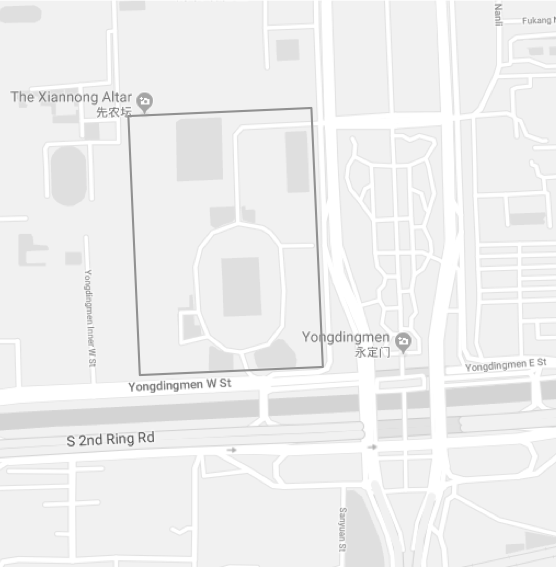
\includegraphics[width = \linewidth]{images/beijingXNT.png}
  \caption{Location of the Temple of the God of Agriculture Sports Technology Institute  (Source: Google Maps)}
  \label{fig:beijingXNT}
\end{figure}


\begin{figure}[htbp]
  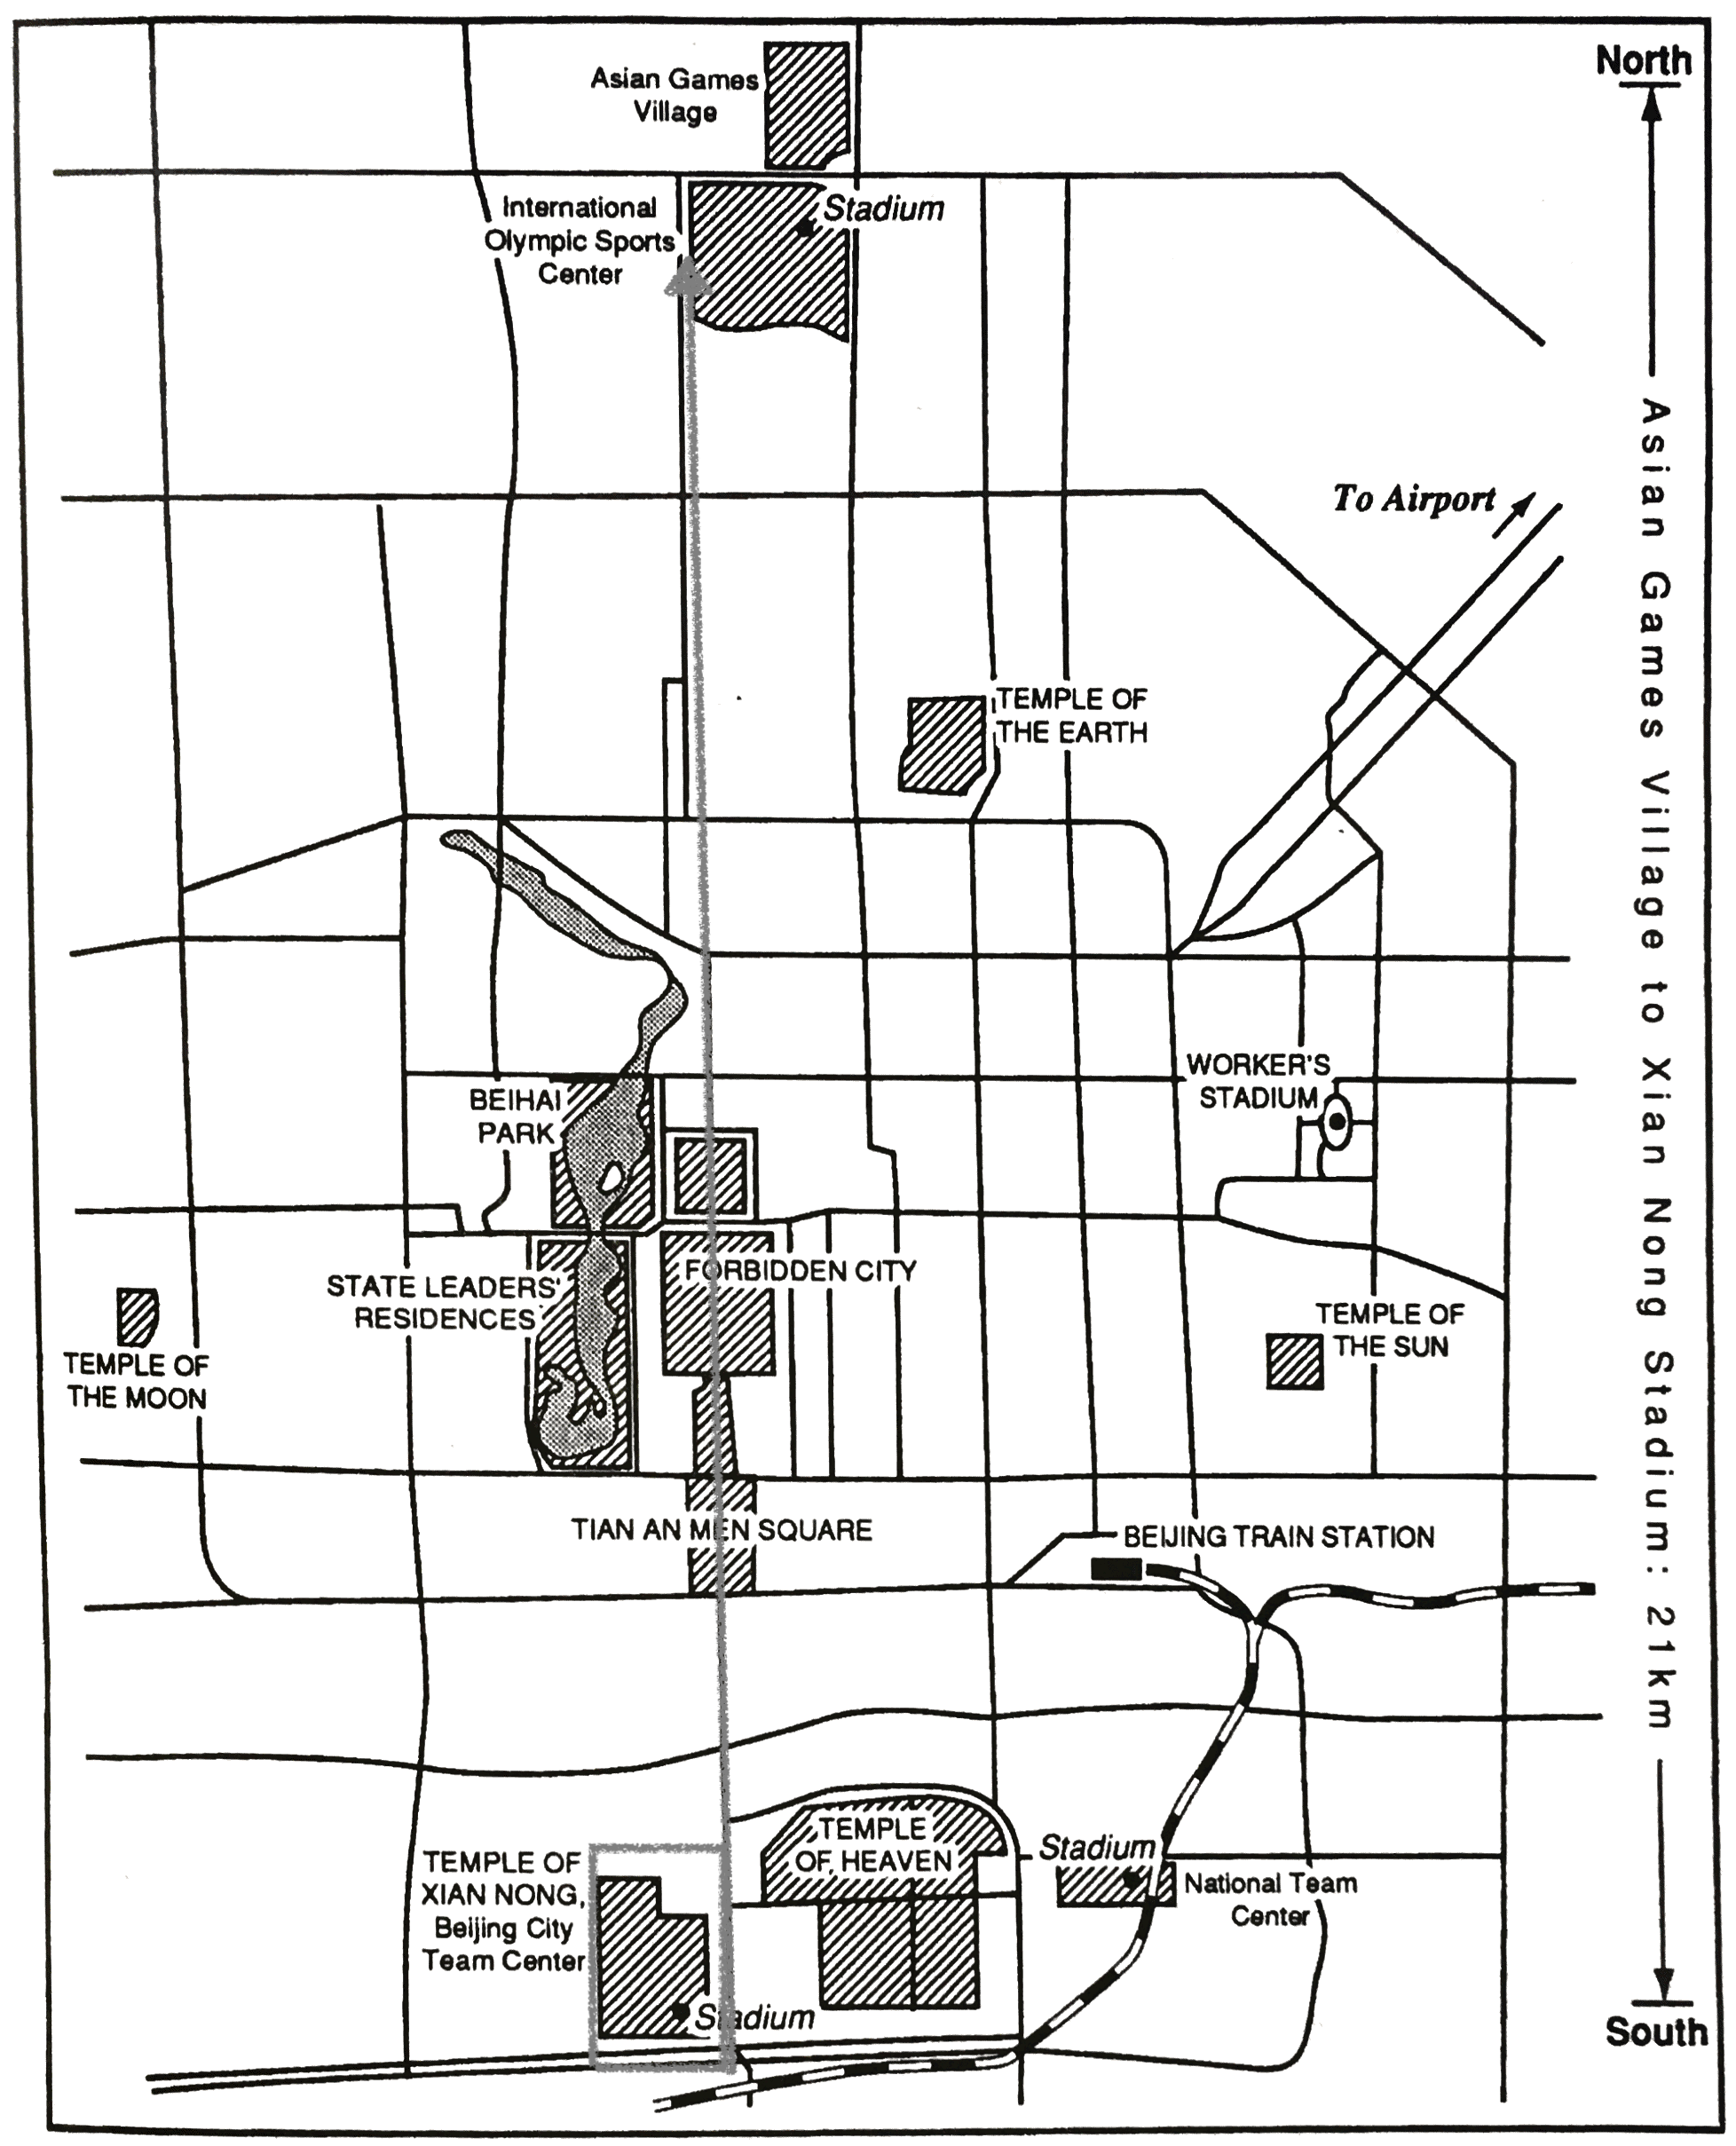
\includegraphics[width = \linewidth]{images/beijingTemplesXNT.png}
  \caption{Locations of former Qing dynasty temples (Brownell 2008)}
  \label{fig:beijingTemplesXNT}
\end{figure}


\section{Introduction}

The core assertion of this dissertation is that a scientific explanation of the cross-cultural prevalence of group exercise in pre- and post-Agricultural human societies must pay greater attention to the system dynamics and component cognitive mechanisms of joint action. Existing experimental evidence linking group exercise and social cohesion is derived predominantly from laboratory experiments in which essentialised dimensions of group exercise---namely, behavioural synchrony and physiological exertion---are manipulated within dyads or small groups.  Results of these studies indicate that various forms of synchronised behaviour (from tapping to walking to rowing to talking) and physical exertion are independently responsible for generating pro-social behaviour. It has been hypothesised that a range of cognitive and neuropharmacological mechanisms generate a psychophysiological environment conducive to social affiliation and in-group cohesion.

As outlined in detail in Chapter 2, sporting anecdote has for some time pointed to the importance of team click in processes of affiliation and team cohesion.  Particularly in the case of highly skilled practitioners, the ecstasy of group activity is contingent not on mere participation in joint activity, but on the perceived achievement of fine-grained alignment of behaviour with co-participants.  The psychology of flow offers support for this dimension of reward associated with peak athletic performance, although scientific knowledge of flow states remains heavily restricted to individual-level neurocognitive and psychological processes.  A combination of 1) a recent paradigm-shift in cognitive science away from static input-output computational models of information processing towards ``active'' inferential models based on mechanisms of prediction and free-energy minimisation, and 2) empirical research programs dedicated to broadening the frame of analysis of social cognition to include interactions involving the affordances of distributed throughout the brain, body, and the social and physical environment have begun to confirm elements of intuition and anecdote related to the phenomenon of team click.  There is evidence to suggest that the perception of tacit understanding, atmosphere, and general order of coordination with others could be due to the activity of a suite of cognitive mechanisms that range from lower level sensory perception and discrimination processes, to formulating self and other action plans, to representation of joint goals.  Evidence also suggests that these joint action specific processes bootstrap on lower-cognitive mechanisms associated with movement regulation.
Studies involving skilled practitioners in particular reveals a capacity to co-regulate movement in joint action such that joint action resembles an functional interpersonal synergy.  Such coordinative structures can be understood as extra-neural mechanism for minimising cognitive free energy in complex interactional environments, and there is evidence to suggest that the formation and successful regulation of interpersonal coordinative structures is associated with a regime of neuropharmacological reward.  In sum, it appears that in some instances, what is crucial to the ``social high'' of group exercise is not mere participation, but the \textit{quality} of participation, and the perceived click of action with co-participants.

A key insight revealed by the paradigm shift surrounding the social cognition of joint action is the contextual sensitivity joint action (or any cognitive process for that matter).  Joint action does not---in real world situations at least---exist in a vacuum, but is rather heavily contingent upon the informational affordances of the ecological niche in which it is situated.  As discussed in detail in Chapter 2, shared cultural knowledge often serves to set the macro-contextual frame for joint action, acting as a ``coordination smoother'' (SOURCE) that facilitates more effective and efficient synergy formation. In the predictive coding paradigm, cultural habits and affordances act as ``hyper-priors.''  Thus, all levels---from the micro-level predictive processes associated with movement action and perception, to the macro-level predictive frames offered by specific cultural and contextual niches---are relevant to the outcome of joint action.

This paradigm shift in social cognition accords neatly with anthropology's traditional oncern for honouring the distinctiveness of any given cultural niche, and offers an opportunity for reconciliation between anthropology and cognitive science \citep{Whitehouse&Cohen}. As the lessons from WEIRD attempts of cultural psychology have exposed, action must be understood within the context of a specific cultural trajectory, and generalisable mechanisms must be located within culturally-specific terrain.

Ethnography is thus perfectly placed as a first step.
unveil under-theorised dimensions (team click)
generate hypotheses
Then step-wise testing of mechanisms which have been callibrated to the specific context.

This dissertation honours the importance of in-depth:
(from abstract)


In this chapter, I outline:
JA, Team Click, SB in
  - Rugby
  - China

History of physical activity and rugby in China

Outline qualifications for research

Re-calibrate predictions based on this contextualisaton work


















A combination of sporting anecdote and evidence emerging from social cognition of joint action involving expert practitioners suggests that the ``social high'' associated with group exercise contexts may crucially depend ong the extent to which joint action prescribed and performed in a particular context ``clicks'' with participants' prior expectations.  In this sense, the mere presence of synchrony and exertion may be a necessary but not necessarily sufficient condition for the resultant ecstacy observable in group exercise context. Social cohesion  %. There is also some evidence that these variables may interact \citep{Jackson2017}.


Group exercise appears in a diverse range of human activities within and across cultural and historical contexts, spanning music making, ritual practices, warfare, play, and modern sport.  Current research suggests that group exercise confers individual-level benefits ranging from increased physical and mental health (including reductions in stress and anxiety) \citep{}, reductions in pain and fatigue \citep{Cohen2009,Davis2018}, and could be responsible enhanced cognitive \citep{} and athletic \citep{Davis2015} performance.  It has been proposed---based on evidence in the archeological record and the observation of analogous behaviours in non-human primates (e.g., group hunting in Chimpanzees)---that the benefits of group exercise can be understood in terms of an ancestral past in which persistence hunting, travel, communication, and defence were of key relevance to survival \citep{Sands2010}.

It is also generally agreed that the persistence of group exercise following transitions to agricultural modes of production in the Holocene (11ka) can be best understood in terms of processes of social cohesion and cultural group selection \citep{Dunbar2010,Whitehouse2004,Cohen2017}.  In this account, the cognitive and neuropharmacological mechanisms associated with coming together and moving together may be part of the ``social glue'' that functionally binds teams, religious communities, or concert-goers \citep{Cohen2009,Fischer2014a}.  Under the assumption that more cohesive social groups outperformed less cohesive groups in our evolutionary past \citep{Turchin2013}, the binding effects of group exercise may be a causal factor directing population-level transmission and fixation of biological and cultural variants that continue to support a capacity for group exercise \citep{Claidiere2014,Henrich2015}.

But many details of this account remain poorly understood.  As I outline in Chapter 1 and 2, for example, evolutionary accounts of group exercise lack an understanding of how properties pertaining to the physical coordination of movement within and between human bodies and minds enables functionally coordinated assemblages and long-term coherence and stability of bodies, minds, and collectives.  In short, the science of physical movement coordination, also known as ``Coordination Dynamics'' \citep{Kelso2009} is an example of an empirical research domain that challenges the limits of a single-level and unilateral causation model of evolutionary change, in which a pact between population-level gene frequencies and natural selection directs phenotypic variation \citep{Dawkins1976,Grafen1984}.  Movement coordination is a dynamical process that could a constructive force in the creation and maintenance of adaptive niche ecologies over multiple generations.  It appears to be due to 1) the rigidity of MS theoretical predictions, and 2) the methodological challenges associated with quantifying properties of coordination dynamics, that the role of movement coordination in group exercise has until now failed to be considered as an important causal process linking joint action of group exercise with social cohesion.

% social cognition of joint action:

% multi-level scaffolding: priors, coordination smoothers, hyper-priors subject to cultural attraction...
habits of activity
cultural milieu
evolutionary niche

% study predictions:
%





In the sections that follow in this chapter, I establish the historical and cultural context of the present study, including my unique qualifications as researcher that facilitated data collection.

\section{Introducing the joint action context: Rugby union in China}


\subsection{Joint action, team click, and social bonding in rugby}

  \subsubsection{Rugby Union}
    % P: Rugby is a good choice for JA
    %  F: JA parameters
    %  F: Association with SB
    % E:
  Rugby Union (hereafter rugby) is an interactional team sport played on a rectangular field (100m x 70m), by two teams, usually of 15 players, who physically contest possession of an egg-shaped ball that can be used to score points \citep{IRB2014}.  Descending from a variety of locally-specific folk-games played in pre-industrial England, all loosely grouped as ``football'', rugby developed within the elite public school system as a deliberate physical activity arbitrated by rules and regulations, before circulating through the arteries of England's colonial empire as a leisurely pastime—a ``sport'' \citep{Dunning2005}.  In 1996, rugby became a professional sport and is played as such in Western Europe and in the Southern hemisphere. Rugby sevens---the specific focus of this dissertation---is a modified version of the conventional 15-a-side game involving teams of 7-a-side (rather than the conventional 15), and 14-minute games played in a Tournament structure over two or more days (rather than a one-off 80-minute match between two teams).  Rugby sevens has grown in popularity more recently, particularly since its introduction to the Olympics for the 2016 Games in Rio de Janeiro.  More so than the traditional version of the game, rugby sevens is played by countries all over the world, and attracts more balanced participation by men and women.

  Rugby sevens is a highly interactive and physiologically demanding sport at all levels at which the game is currently played. Sevens requires players to participate in frequent bouts of intense activity at and above the aerobic threshold such as sprinting, physical collisions, tackles, and grappling, separated by short bouts of low intensity activity such as walking and jogging. Rugby requires high levels of interdependence between team members due to the uncertainty and complexity of interactive coordination tasks.  At the elite level in particular, the physiological costs and complexity of joint action requirements of rugby are amplified.




Rugby, like many equivalent team sports in which a single ball (or similar object) is contested such as basketball, association football and ice hockey, is made up of a series of sub-phases involving attacking and defending sub-units \citep{Passos2011}, and requires its athletes to perform and continually repeat similar joint actions with teammates.   The highest order of joint action in rugby sevens consists of 14 athletes (7 per team) who coordinate around the shared goal of completing a 14 minute game in which one team competes against the other team for victory.  Within this overarching frame, lower-order goal-directed joint actions are nested.  Depending on which team is in possession of the ball, players coordinate their movements around shared goals of attack or defence.  Completing the goals of attack and defence usually require coordination between sub-units of 2-4 athletes per team.  The goal of attacking subunits is to penetrate the defensive line or to at least advance towards the opposition's try line by securing possession at the ``breakdown'' (the contest for possession that occurs after a ball-carrier is tackled and brought to ground) in order to score points during a later sub-phase of attack.  The goal of the defensive subunit is to halt the ball-carrier and subsequently successfully contest possession of the ball at the breakdown.

  %P: finely tuned calibration of behaviours in environment of high uncertainty
There is evidence to suggest that dynamic coupling occurs between dyads and sub-units of attack and defence\citep{Passos2011,Correia2014}.  Passos and colleagues \textcite{Passos2011} for example find that functional coupling tendencies emerge between attacking dyads and adapt to specificities of the task environment.  Correia and colleagues \textcite{Correia2014} show that coupling tendencies also emerge between co-actors of opposing teams in rugby union, for example, in a 1-on-1 attacker/defender sub-phase.  These results are confirmed in similar joint action contexts in other equivalent sports such as basketball and association football \citep{Duarte2013}. There is evidence to suggest that the establishment and maintenance of functional  interpersonal synergies in rugby joint action depend on an athlete's perception of affordances of the task-specific cognitive system made up of constraints including other athletes, the physical environment, and the rules of the game \citep{Passos2012}.

% P: Cognitive threshold for maintaining social bonds
Dunbar \textcite{Dunbar1992} proposes that the ratio of human neocortex size to total brain volume imposes an upper cognitive limit on realtime coordination of behaviour of  4-5 individuals.  The group size of joint action sub-phases and sub-units in rugby sevens (2-4) fall within this upper limit, or just above the upper limit if attacking and defending subunits are grouped together (4-8).  Each team of 7 is complemented by a further 5 reserves to make up a total squad of 12 who compete in a tournament setting.  In addition, the size of squads that train together outside of tournaments can range anywhere from 16 to 28.
These group sizes also exist within the cognitive limits for maintaining face-to-face intimate relationships, thought to be in the realm of 15-25 \citep{Dunbar1992,Dunbar2010}. These specific requirements of joint action in rugby sevens suggest that neurocognitive mechanisms responsible for tracking and monitoring coordination between co-actors and establishing interpersonal synergies between co actors will be particularly relevant \citep{Mogan2017}. (In addition to neuropharmacological mechanisms)

There is very little direct empirical evidence specific to rugby union that can be used to substantiate a link between joint action and team click, and team click and social bonding.  Despite this, rugby is a sport heavily associated with the popular interpretation of ``social bonding,'' particularly in all-male social organisation common in the elite educational spaces of England and Commonwealth countries in which rugby originally developed \citep{Dunning2005,Richards2007,Collins2008}.\footnote{Recently, rugby union has been the site of much criticism due to the fact all-male social spaces cultivated by rugby appear to support and sustain hyper-masculine and hyper-normative behaviours, including gender-related violence \citep{Cosslett2014}.

``Rugby is a game for barbarians played by gentlemen,'' or so the saying goes.\footnote{The origins of this oft-cited Rugby adage is unclear.  The phrase is supposedly the adopted motto of the British Barbarians Football Club, established in 1890 \citep[34]{Dunning2005}.  The complete phrase reads ``Rugby is a game for barbarians played by gentlemen, football is a game for gentlemen played by barbarians.''  However, official club history cites its original motto as, ‘Rugby Football is a game for gentlemen in all classes, but for no bad sportsman in any class' \citep[vii]{Starmer-Smith1977}.  Some sources attribute the saying to British writer and poet Oscar Wilde (1854-1900) \citep{Fleenor2015}}. Different inflections on this adage have been reproduced by people in all parts of the world that rugby has reached (including China \cite{}), presumably as a way of linking the nature of rugby's physical requirements with social virtues of fair play, cooperation, and moral integrity. For example, the current slogan of World Rugby, the international governing body of rugby union, is ``Building character since 1886'' \citep{WorldRugby2017}, referring to the moral character that can be generated through participation in rugby union.  In this case the physiological demands, joint action complexity, and social-historical trajectory of rugby suggests that it is extremely suited to an investigation of the social bonding effects of group exercise.



  \subsection{Joint action, team click, and social bonding in  China}


  \section{Cultural Variation}
  In addition to micro-level details and dynamics of joint action, macro-level variation in the cultural contexts of joint action also vary extensively. Importantly, macro-cultural expectations appear to frame and direct micro-level movement dynamics of joint action.  As sporting anecdote indicates, different teams from different places and times appear to play the same game in very different ways---embodying different ``styles'' of play.  While there is very little literature devoted to examining the effect of cultural variation on joint action and social bonding in particular, there is extensive evidence to suggest that cultural variation impacts on processes of cognition \citep{Nisbett2003,Hoshino-Browne2005}, social learning \citep{Mesoudi2015}, and prosocial behaviour \citep{Yuki2005,Yuki2003}.
  It has been suggested that cultural environments structure joint action scenarios in ways that help ``smooth'' coordination by providing equivalent expectations between co-participants \citep{Vesper2017}.  Indeed, as anecdote and observations concerning suggest, perception of ``team click'' is not necessarily limited to the most proximal dimensions of joint action perception, but is rather contingent on the snug fit between a given joint action and a whole assemblage of hierarchically ordered expectations.\footnote{It is also important to bear in mind that, while the neurological, cognitive, and psychological theories from which the predictions of this dissertation strive for universal generalisability, these theories are nonetheless heavily grounded in Western epistemological assumptions, intuitions, and ``WEIRD'' empirical evidence \citep{Henrich2010a}.}
    Non WEIRD setting
    Cultural cognition as a ``factor of attraction''
    Cultural hyper-priors that structure joint-action and constrain active inference (Clark 2013) <-- coordination smoothers

  \subsection{Cultural cognition as a factor of attraction}

  Cultural Modes of group membership and social cognition:

  An analysis of literature concerning the cultural psychology of self-construal can provide important insights into the way in which macro cultural processes interact with micro-dynamics of social interaction to structure and constrain cognitive processes implicated with joint action, team click, and social bonding.  As Anthropologists have emphasised for some time \citep{Strodtbeck1961,Kluckhohn1961,Mead1967,Fei1992}, and as cultural psychologists are now beginning to demonstrate in experimental paradigms, processes of group membership appear to vary cross-culturally \citep{Markus1991,Nisbett2001}.  Based on recent cross-cultural research, social and cultural psychologists have developed a theoretical spectrum of group membership processes, the two poles of which can be described as categorical and relational \citep{Hofstede1980,Brewer2007}.  Whereas some cultures, traditionally ``Western'' cultures such as the US, the core of self-definition is based on individual autonomy and separation from others.
  The self-concept of relational societies, traditionally understood to be predominantly East Asian cultures, by contrast, is defined primarily based on social embeddedness and interdependence with others comprising their in-groups\citep{Leung2012}.

  Unsurprisingly, much of Anglo-American social psychology of the 20th Century is rooted in a categorical mode of representing and measuring group membership.  The canonical self-categorisation paradigm of social psychology \citep{Turner1987}, for example, requires that a bounded individual (experimental subject) make an identification between abstract categories of the self and the in-group or out-group.  Categorical group membership is thus achieved when the perceived differences between the self and other in-group members are smaller than the differences between in-group and out-group members \citep{Yuki2014}.  In distinction to a categorical mode of group membership, relational group membership involves attention to maintaining and harmonising intragroup relationships, engaging in intergroup categorical comparisons \citep{Yuki2003}.
  In a relational mode, social identity is less a function of distance between abstract categories of self and in-group, and more a degree of commitment to cultivating a network of hierarchically structured---but more or less self-centred and self-enhancing---network of relationships \citep{Liu2009,Nisbett2003}.

  These two predominant modes of group membership—--categorical and relational—--have been shown to vary across cultures (i.e. East Asian versus Western European or North American, see \citep{Markus1991,Nisbett2001,Yuki2003}, within groups (according to sex and personality differences \citep{Yuki2014}, and indeed, within individuals (depending on contextual and situational primes, \citep{Lee2014,Wong2005}).  While the durable persistence of cultural and linguistic institutions appear to be responsible for the prominence of one mode of membership over another (East versus West, for example), recently researchers have suggested that divergent modes of group membership—categorical and relational—may be mediated by context-specific socio-ecological factors such as the level of relational mobility in any given environment \citep{Oishi2010,Takagishi2014,Yuki2005}.  Both modes of group membership have been shown to shape attention, cognition, and behaviour \citep{Nisbett2003} and as such have important implications for the task of identifying and measuring social bonding mechanisms of joint action

  Experimental evidence suggests that categorical group processes facilitate fast and effective identification with arbitrary minimal groups \citep{Diehl1990,VanBavel2014}, the arousal of intrapersonal cognitive dissonance between the self and experimentally constructed in-group \citep{Festinger1957, Stone2001}, higher levels of cooperation with categorically similar strangers in economic games \citep{Yuki2005,Yuki2003}, and greater attention to and memory recall \citep{Buchan2006,Ng2016}.  In cultural environments where relational processes of group membership are more prominent or salient, on the other hand, the inverse is usually observed. First, minimal group paradigms have had very little (if any) success in East Asian (particularly Japanese) contexts \citep{Liu2009}.  Relational group processes, on the other hand, allow for the arousal of cognitive dissonance only when it is constructed interpersonally (as opposed to intrapersonally) between an individual and specific individuals to which that individual is connected by a meaningful social relationships \citep{Hoshino-Browne2005}.  Likewise, individuals with a predominantly relational group awareness are more willing to cooperate with and attend to strangers with whom they share relational rather than categorical ties \citep{Ng2016,Yuki2005}.

  Relational group membership has a long history in China, rooted in Confucian \citep{Hwang1999}, folk-cultural axioms \citep{Wang2009}, agricultural modes of production \citep{Talhelm2014,Fei1992}, dynastic rule, and modern reinventions of these cultural forms by processes of the nation-state\citep{Liu2014}. The metaphor of the family is particularly salient and pervasive in modern public representations.  On almost every scale of social organisation, from dyadic extra-kin friendships through to workplace interactions and macro-social organisations (cities, provinces, nation), the family and its relational priorities are consistently invoked to aid coordination and coerce participation in collection action.
  In addition, the last 150 years of Chinese modern history has also entailed the introduction of categorical group processes associated with the activities of the nation-state, leading to a contemporary Chinese indigenous psychology in which a relational mode is predominant, and a categorical mode is contextually-activated, especially when categories such as ``China'' are threatened or challenged internationally \citep{Liu2009}.


  \subsection{Joint action, team click, and social bonding in China}
  As mentioned above, while there is very little empirical evidence linking movement coordination and social bonding within the Chinese cultural context, there is extensive indirect evidence from historical and contemporary literatures to suggest ways in which this relationship---between (joint) action and social processes of group formation and cohesion---is uniquely articulated in the Chinese context \citep{Weed2011}.  Historical evidence also suggests that the dynamics of joint action in particular have the focus of ethical considerations, namely resolution of social tensions inherent in collective action problems \citep{Slingerland2014}.

  It is well documented that the most prominent metaphor in Chinese cultural discourse is that of the family \citep{Maehr1980}, and that this metaphor structures many extra-kin social relationships between individuals, and between the individual and the state \citep{Gold2002}.  Traditionally, the father-son kinship relationship is utilised to naturalise the socially constructed relationship between lord and minister: ``Parents naturally love their children, and children naturally love and respect their parents, and they both know that they're stuck with one another no matter what...'' \citep[178]{Slingerland2014}. Likewise, the metaphor of family is often utilised to naturalise the notion of an extra-kin social group, for example a company or a sporting team \citep{Brownell2008}.
  It is important to emphasise that, whereas traditionally Western (Anglo-American) notions of group membership generally hinge upon a psychological representation of egalitarian equivalence between categories of self and group, the utilisation of the family metaphor for group processes relies on the individual identifying group membership through a participation in hierarchically structured (familial-like) \textit{relationships} \citep{Fei1992}.

  It is within these processes of extending familial metaphors to formal social relationships that Slingerland (2014) locates a key role for joint action. Inherent in the scaling up of familial relationships to extra-kin social relationships is the tension common to many collective action problems, that of vulnerability to free-riding and defection \citep{Cosmides2013,Gavrilets2015}.
  As Slingerland explains, the ``logic of civilised life makes us very keen to distinguish reliable cooperators from unreliable defectors...what we want then is a particular type of desirable...behaviour where there is absolutely no gap between action and motivation'' \citep[192]{Slingerland2014}. The paradoxical Chinese idiom of \textit{wei wuwei}, translated awkwardly into English as ``trying not to try'' or ``effortless action,'' is promoted in many ancient Chinese philosophical corpuses as a behavioural solution to conflicting incentives involved in coordination problems: effortlessness in performing socially desirable actions (virtues) communicates a level of mutual trust and commitment that is ``hard-to-fake.''  The phenomenology of effortless action is described at length in many of these corpuses, and is a key dimension of many traditional Chinese martial arts such as Taichi and Wushu \citep{Morris1998}.
  While mass participation in Anglo-American competitive sports is only a recent phenomenon in China \citep{Brownell2008}, the social valorisation of certain types and styles of movement, particularly the phenomenology of flow in (joint) action appears to enjoy a long history.




\section{Historical Context of rugby in China}

\subsection{Physical activity in Chinese modern history}
The history of Sport and exercise in China is in many fascinating ways emblematic of broader---often fraught and turbulent---processes associated with China's modernisation.  Beyond physical cultures indigenous to China, or practices imported much earlier in history from south Asian religious traditions (e.g. Buddhism and Hinduism), the emergence of Anglo-American interactional team sports and European calisthenics in China is entangled with a history of interaction, conflict, and embrace with foreign influence during the 19th, 20th, and 21st centuries.

  \subsubsection{Introduction, rejection, and embrace of sport and exercise in China 1842-1912}
By the beginning of the 19th century, China had established flourishing international trade relationships with Western empires.  Generally speaking, China traded in tea, silk, and porcelain, meeting high demand in emerging middle class households of newly industrialised nations of England, France, and Germany.  In return for these goods,   merchants from Western empires initially paid in silver, until it became clear that a trade imbalance was emerging between China and the West, owing to the fact that tea, silk, and porcelain where much more replenishable than silver \citep{Fay2005}.  Thus, by the late 19th century Western powers increasingly sought alternatives to silver, for which opium provided a much more replenishable (and addictive) solution.  By the mid-19th century, however, a series of conflicts arose between Qing dynasty rulers and the Western empires over the regulation and trade of opium, leading to the first Opium War (1939-1942).  The resulting Treaty of Nanking (1842) initiated a period of colonial occupation of China that drastically weakened the political power and legitimacy of the Qing Dynasty and increased the influence of foreign powers within China's major inland and port cities.

Increased foreign influence in China during this period brought with it the introduction of an array of ideas and practices to China's urban elite ruling classes, including novel physical cultures of dress, adornment, leisure, and exercise.  Increasingly popular at the time in Europe and North America was the belief that sport and exercise were important pedagogical tools in the development of physically and mentally strong subjects of post-Enlightenment modernisation \citep{Elias1986}.  This belief largely gelled with the values of a nationally (and internationally) motivated Chinese urban elite, and subsequently manifested in China in the promotion of Anglo-American competitive sports by North American Christian missionary organisations such as the YMCA (Young Men’s Christian Association), and the incorporation of calisthenics routines into military exercises \citep[240]{Morris2004}.  Such techniques were soon popularised within elite intellectual communities as pedagogical tools designed to foster an explicit link between the strength of the physical body and the strength of the Chinese nation \cites[32]{Morris2004}[49]{Brownell1995}.

The introduction of novel political ideas to China in the late 19th century involved importation \textit{en masse} of novel linguistic, cultural, and social categories and practices from the West and Meiji Japan (1868-1912) \citep{Liu1995}. \textit{Tiyu} (体育), the term in modern Chinese that most closely translates to sport, was one of many neologisms inherited from the Western social sciences via its Japanese translation.  Importantly, tiyu encompasses more than just the modern Anglo-American competitive sports (roughly translatable to ``yundong'' (运动) that the English word connotes.  Instead, the modern Chinese notion of sport refers to an entire culture and discipline of the body that is deeply intertwined with the political project of Chinese modernisation and advancement \citep{Morris2004}.\footnote{As Lydia Liu (1995: 58) points out, even the notion of “China” itself as a term linked to a national imaginary, only began to emerge as such through interaction with Western missionary discourses concerning ``China'' during the 2nd half of the 19th century.}

The two-character phrase \textit{tiyu} is a contraction of a longer four-character phrase \textit{shenti jiaoyu} (身体教育), a direct translation of Herbert Spencer’s notion of  ``a physical education'' that first appeared in Chinese reformist intellectual Yan Fu’s ``On Strength'' 1895 \citep[9-10]{Morris2004}.  Now naturalised within the modern Chinese vernacular, compound words such as the ``body'' (\textit{shenti} 身体) and ``education'' (\textit{jiaoyu} 教育), as well as other fundamental conceptual social categories such as ``society'' (\textit{shehui} 社会) and ``culture'' (\textit{wenhua} 文化) all first appeared in their modern form as an arsenal of translated neologisms made popular by Chinese intellectuals in the late 19th and early 20th century who were grappling with ways to transform a dynastic realm crippled by colonial occupation and feudal backwardness into a strong nation in a system of modern nations \citep{Pusey1983;Schwartz1964;Liu 1995;Huters2005}.   Convinced that the body, \textit{shenti}, was crucial to realising this transformation, intellectuals rigorously subscribed to the Spenserian ideal of a physical education, which combined with a moral and intellectual education, as a ``cultivation of the whole moral, intellectual, physical, and aesthetic self'' (\textit{dezhitimei quanmian fazhan} 德智体美全面发展) \citep[10]{Morris2004}.

%\subsubsection{The Boxer Rebellion}
Novel regimes of sport and exercise were not uniformly embraced in China during this period, however.  The most organised movement of anti-foreign, anti-colonial, and anti-Christian resistance during the period 1842-1912 came in the form of an army of Chinese subjects from rural areas of Shandong was known as the ``Militia United in Righteousness'' (\textit{yihetuan} 义和团).  The Militia trained in martial arts and meditation and explicitly rejected Western forms of physical culture such as sport and exercise \citep{Brownell2008}.  The Militia's first target in the ``Boxer'' Rebellion (1900-1901, members of the Militia were known in English as the ``Boxers,'' due to the fact that they had been practitioners of martial arts that included boxing) was the Horse Racing track in Beijing situated at the south gate of the Temple of God of Agriculture---a site that had become heavily associated with the activity and influence of foreign legions.

In a somewhat harsh twist of fate for the Militia, the influence of modern sport infiltrated Beijing's sacred sites even further in 1901, when the troops of the Eight-Nation Alliance (United Kingdom, The United States of America, Germany, Japan, Russia, Italy, and Austro-Hungary) arrived in Beijing to relieve the besieged international legions.  During this period, troops from the UK occupied the Temple of Heaven to the east of Yongding gate, while US troops occupied the Temple of Agriculture to the west \citep{Brownell2008}. Compared to many other open public spaces in Beijing, the flat, open spaces of Beijing's temple grounds were conducive to the playing of Western sports common in garrison life such as field hockey and association football.  Throughout the final years of the Qing Dynasty, the sporting activities organised within the grounds of the Temple of Heaven and Temple of Agriculture attracted the participation of troops from other legions, as well as western missionary organisations such as the YMCA, and local Chinese elites \citep{Steel1985}.


\subsubsection{Republican Era (1912-1949)}
The combination of a weakened dynastic regime and the influx and development of new political and social ideas among China's urban intellectual elite led eventually to the Chinese revolution in 1911, and the establishment of the Republic of China (ROC) in 1912 \citep{Mitter2008}. Sport in China began to develop among urban elite along two main strands—--``competitive sports'' (\textit{jingji tiyu} 竞技体育) and ``games and calisthenics'' (\textit{ticao} 体操).  Traditional Chinese martial arts also made a resurgence during this period.  Although initially delegitimised within the New Culture Movement as elements of feudal superstition, members of the National Essence Movement (\textit{guocui yundong} 国粹运动) reappropriated martial arts to by aligning these practices with rational modernist ideas about sport and the body, at a time when sport became more significant for the articulation of an emerging national identity in the face of imperial powers \citep[38]{Brownell1995}\citep[45]{Morris2004}.  A significant aspect of competitive sports was the public spectacle of the ``games meets'' (\textit{yundonghui} 运动会), in which the performance of emerging national and international political identities could take place.  As early as 1908, the Chinese sport community enshrined the Modern Olympic Games (\textit{Aolinpike yundonghui} 奥林匹克运动会) as the pinnacle of participation in an international community of nations, and as such, the quadrennial global ritual has since preoccupied a collective Chinese sporting consciousness, and a Chinese national consciousness more broadly (\citep{Burnett2009;Barme2009;Brownell2008;Morris2004;Xu2008}.

The most sourthern point of Beijing's sacred north-south continued to feature prominantly in the development of sport in the ROC.  In 1914, the YMCA organised the first ever multi-sport event within the walls of the Temple of Heaven in Beijing, which the ROC nationalist government later labelled the Second National Games (the label of the First National Games of the Republican era was retrospectively assigned to the ``First National Athletic Alliance of Regional Student Teams'' multi-sport event hosted by the YMCA in Nanjing in October 1910) \citep[441]{Li2015}. The active reappropriation of the sacred spaces of the Qing Dynasty through activities such as team sport, allowed the foreign legions to perceive their occupation of these sites as a demonstration of superiority over the Qing court, and facilitated the ROC's priority of displacing traditional reverence of the throne \citep{Hevia1990}.

Beijing lost its importance as the centre of state power when the ROC moved the capital to Nanjing between 1928-1948.  In 1937, however, after the space surrounding the Temple of Agriculture had been repurposed for a range of leisure and amusement activities (including sport), a large sports stadium was constructed on the land directly to the south east of the main altar.  With a capacity of 10,000 people and a dirt association football field in the middle, the Beiping Public Stadium (as it was originally named) was the second ever modern sports stadium to be built in the ROC---the first being built two years previously in Shanghai for the hosting of the National Games in 1935.  The grounds immediately surrounding the stadium subsequently became the site for the Beijing Municipal Elite Sport Training facility, the predecessor to the current Institute.


\subsubsection{Sport in the People's Republic of China (1949-1976)}
Sport was transformed and politicised in radical ways following the establishment of the People’s Republic of China (hereafter PRC) in 1949.  As a key member in the New Culture Movement and the May Fourth Student Revolution, CCP leader Mao Zedong was a proponent of the Spenserian logic of physical education.   When the CCP took power in 1949, the centralisation of the proletarian body and the propagation of an ideology of active body-cultivation was such that \textit{not} ``training the body (for China)'' was considered bourgeois and therefore anti-nationalist \citep[58]{Brownell1995}.  The body of the worker (\textit{gongren} 工人), peasant (\textit{nongren} 农), and soldier (\textit{bingyuan} 兵员), as well as the body of the athlete (\textit{yundongyuan} 运动员), were glorified for their ``capacity for manual labour'' (\textit{laodongli} 劳动力 )---the ideological foundation for the ``proletarian revolution'' (\textit{wuchanjieji dageming} 无产阶级革命) (Ge and G. 2005: 91).  The ``emancipation ''(\textit{fanshen} 翻身) and glorification of the physical, labouring body is particularly explicit in the propaganda posters of the early Mao era (Ge and G. 2005: 87) (see Figure ~\ref{fig:motherlandStrength}).

    \begin{figure}[htbp]
      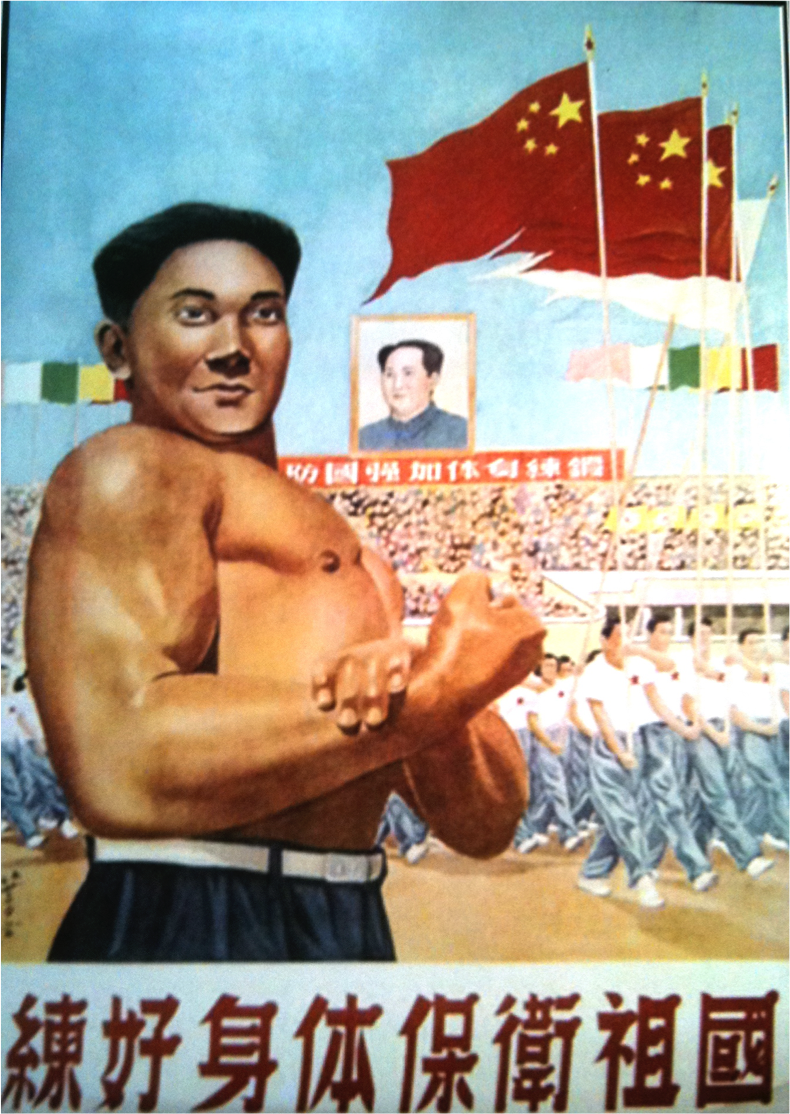
\includegraphics[width = \linewidth]{images/motherlandStrength.png}
      \caption{Strengthen Physique to Defend Motherland (1950)}
      \label{fig:motherlandStrength}
    \end{figure}


Along with many other facets of society after 1949, sport was institutionalised in line with Soviet bureaucratic models of governance.  In 1952 the ``State Sports (and Physical Culture) Commission'' (\textit{guojia tiyu yundon wieyuanhui} 国家体育运动委员会) (hereafter the Sports Commission) was established, which acted as the central State organ responsible for the administration of ``sport for the masses'' (\textit{qunzhong tiyu} 群众体育), ``physical culture education'' (\textit{tiyujiaoyu} 体育教育), as well as an elite competitive sport (\textit{jingji tiyu tixi} 竞技体育).  The competitive sport system was designed with the intention of creating a fast track for the development of world class athletic talent, in lieu of sports systems of western countries whose development pathways for athletes were more organically embedded within existing social and educational institutions. By creating model athletes capable of performing and advocating the healthy, egalitarian and militaristic body promoted by the Party, competitive sport was designed to kick-start more widespread engagement in ``sport for the masses'' and ``sport education''\citep[56]{Brownell1995}.

At the bottom of the hierarchical structure of the Sports Commission are local sports commissions (county, township and city), above which are the provincial and municipal sports commissions; and at the top is the National Sports Commission, located in Beijing \citep[59]{Brownell1995}.  The Sports Commission was responsible for all sports training centres and sports programs, of which there were many types.  On one extreme, the elite professional arm of the Sports Commission , a ``national (sport) system'' (\textit{juguo tizhi} 举国体制), which presides over all full-time professional sports teams (\textit{tigongdui} 体工队) that exist at national and provincial/municipal levels.  The main objective of this national system is to cultivate elite athletes to compete on a national and international level, in events such as the National Games (\textit{Quanguo yundonghui} 全国运动会), the Asian Games (\textit{Yazhou yundonghui} 亚洲运动会), and most importantly, the Olympic games (\textit{Aolinpike yundonghui} 奥林匹克运动会).  Due to an overwhelming Olympic-focus, all sports under the umbrella of professional arm of the Sports Commission are either Olympic sports, or Chinese martial arts (Guojia tiyu zongju 2009a).  Outside of this professional arm, elite sport programs are embedded within secondary and tertiary education institutions in a number of different ways, under the banner of the ``high school and university sport system'' (\textit{gaoxiaotizhi} 高校体制) (Guojia tiyu zongju 2009a).  At a high school level, elite sports programs are offered at ``extracurricular sports schools'' (\textit{yeyu tixiao} 业余体校), as well as regular high schools who focus on one or two sport programs in particular \citep[59]{Brownell1995}. At a tertiary level, a number of specialist sport colleges operate at national, provincial/municipal and local levels.

The reinstatement of Beijing as China's capital immediately following the establishment of the People's Republic of China in 1949, had immediate implications for the Institute situated at the Temple of God of Agriculture.  The existing stadium was enlarged to a capacity of nearly 30,000, and lights were added to enable hosting training and events at night.  The stadium was host to many important sporting and political events between the years of 1949 to 1976, including a number of International football matches attended by high profile CCP members, including Mao Zedong and Zhou Enlai (see Figure ~\ref{fig:maoXNT}).  Despite becoming heavily entwined with political processes of the PRC during 1949-1976, sport and its development was also severely hampered by many factors during this period.  On the one hand, the internal political, social, and economic chaos of The Great Leap Forward (1955-58) and the Cultural Revolution (1966-77) detracted from a focus on development of sporting infrastructure and sporting development.  On the other hand, PRC's exclusion from membership in the International Olympic Committee (IOC) and thus participation in the Olympic games, limited China's ability to participate in sporting events on the International stage.

\begin{figure}[htbp]
  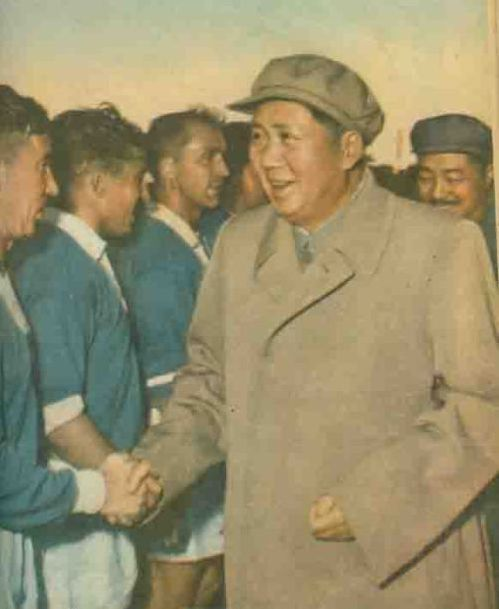
\includegraphics[width = \linewidth]{images/maoXNT.jgp}
  \caption{Mao Zedong congratulating members of the St Petersburg Zenit FC following a fixture against China in 1952}
  \label{fig:maoXNT}
\end{figure}


\subsubsection{Reform era tiyu (1976-2000)}
The death of Mao and the end of the Cultural Revolution in 1976 signalled the beginning of widespread social and economic transformations in China, in which the development of sport was heavily implicated.

Cultural Anthropologist Susan Brownell’s work, ``Training the Body for China'' (1995) was the first and most comprehensive attempt at an anthropology of sport in China. The research that forms the basis of Brownell's monograph was conducted during the mid 1980s at a time when China was only just beginning to interact politically and economically with an international community.


 In reference to the unprecedented success of the Chinese women’s volleyball team in the 1980s, including winning China's first ever gold medal in a team event at the LA Olympics in 1984, Brownell (1995: 86) explains how elite level sport functioned as a crucial symbolic practice for China in the process of ``rejoining the world.''  As a participant in the sports system as a student-athlete herself, Brownell draws on first-hand ethnographic experience of training and existing as subject to the state-administered ``microtechniques of power'' (citing \cite{Foucault1977}) designed to cultivate athletes in post-Mao China.


Brownell interrogates the role of the athlete in the perpetuation of a hyper-visible and generalisable moral order, cast in official terms as a ``socialist spiritual civilisation'' (\textit{jingshen wenming} 精神文明) (1995: 156).  Brownell explains that the position of the athlete in reform era China was one characterised by the tensions and shifts of an ever-transforming social terrain structured by contradictory forces of the state and the emerging logic of the market.

One of the most immediate transformations to effect the Chinese sports system after the death of Mao was the restoration of the University Entrance Examination (gaokao 高考, hereafter gaokao), following the end of the Cultural Revolution in 1976 \citep[198]{Brownell1995}.  School curricula were immediately redesigned around the gaokao, and as a result, schools quickly reduced emphases on sport programs as they were seen to draw student’s attention and energy away from academic study.  A situation thus emerged where the only option for prospective athletes was to attend a specialist sports boarding school in which a scholastic education was not emphasised or was abandoned all together in favour of intense physical training.

Success on an international stage in the early 1980s delayed public scrutiny of this widening gap between education and sport. The The PRC won a total of 32 medals at the 1984 Los Angeles Olympics---its first official appearance at the Olympics since it boycotted the games in 1952 due to a dispute with the Republic of China (now Chinese Taipei) over the use of ``China.''  Importantly, 15 of these 32 medals were gold, and this powerful display of strength on the international stage was an enormous moment for modern Chinese nationalism in the reform era \citep{Brownell2008}.

When China produced a much less impressive performance in the summer Seoul Olympics in 1988, winning only 5 gold medals (and a total of 28), latent public criticism of way in which reform era sport had become isolated from society readily surfaced and a ``crisis in Chinese sports'' was declared \citep[199]{Brownell1995}.  Amidst broader social anxieties concerning not only the alarming quantity of the Chinese population (renkou guoduo 人口过多问题), but also the problem of population \textit{quality} (renkou suzhi 人口素质问题), the athlete in China was problematised as lacking sufficient ``cultural quality'' (wenhua suzhi 文化素质) in accordance with his or her elevated social status as a ``representative'' (daibiao 代表) of the Chinese nation on an ever-expanding international stage (General Administration of Sport 2009a; Brownell 1995: 95).

In response to this public sentiment, in 1988 former army general Wu Shaozu (伍绍祖) was appointed head of national sports commission and tasked with implementing reform measures that would help the ``societization'' of the Chinese sport system. In 1989, for example, the Sports Commission adopted a policy modelled on the US college sports system, of ``combining sport and education'' (tijiao jiehe 体教结合).  In an attempt to move away from a reliance on sport boarding schools and full-time sports training centres for the development of athletic talent, ``high level tiyu programs'' (gaoji tiyu xiangmu 高级体育项目) were embedded within existing stand alone high schools and universities so as to ensure the ``all-round development''(quanmian fazhan 全面发展) of the athlete \citep[203]{Brownell1995}.  As part of an emphasis on a broader range of sports and their perceived potential to facilitate community engagement, international relations, as well as commercial opportunities, various sports programs, including many non-Olympic sports such as rugby, were inducted into the Chinese sports system for the first time\citep[70]{Knuttgen1990}.  Above all, the  democratisation of sports programs to include non-Olympic sports was driven by a persistent faith---built-in to the logic of ``physical culture'' form its inception int China---in the ability of sport to produce citizens of a certain \textit{quality} \citep[7]{Woronov2003}.

Reform measures continued into the mid 1990s. In an attempt to reduce the monopolisation of power and resources in the sports system, in 1993 Wu Shaozu broke up the six major sporting bodies of the Sports Commission into 23 sports management centres, with the ultimate goal of placing every sport under the management of an independent sporting association. In 1994 the first professional Chinese Football League was established, followed soon after by the professional Chinese Basketball League in 1995. In 1998, the Sports Commission rebranded as the General Administration of Sport (hereafter GAS) to accord with this direction of institutional reform.  But, one year earlier in 1997, powers above decided that Beijing would bid for the 2008 Olympics, and as such a subtle shift in focus occurred in Chinese sport that altered the course of reform.  Indeed, once the bid for the Olympics was announced as successful in 2001, sport reform ground to a halt as priority shifted to winning as many gold medals as possible \citep{News2017}.  Wu Shaozu left GAS in 2000, and his two successors Yuan Weimin (袁伟民, 2000-2004) Liu Peng (刘鹏, 2004-2016) did not actively return to the project of reform, continuing to invest in Olympic performance.  Even though many sports had since established independent associations, these associations had to be directly affiliated with one of the 23 GAS has 23 sport management centres. Rugby, for example, was affiliated with the ``Management Centre for Small Ball Sports'' (\textit{xiaoqiu guanli zhongxin} 小球管理中心),which was also home to sports such as golf and ten-pin bowling.

\subsection{Beijing Olympics and the lost decade of sport reform (2001-2012)}
    The lost decade:
    The structure of the sports system exists today largely unchanged, although its name changed in 1998 to “The General Administration of Sport in China” (国家体育总局 Guojia tiyu zongju) (hereafter the Sports Administration).
    Sport system became a space for scandal and corruption:

    Public discontent concerning the persistence of China's narrow performance-focussed sports system was palpable throughout the 2000s.

    CORRUPTION and SCANDAL:
    marred by controversy:
    corruption, match fixing etc
    Doping reports

    Yet, much like Groundhog Day, as was the case in the 1980s, these murmurings remained sufficiently muffled in public discourse by the strong performances of Chinese Olympic athlete delegations in Sydney 2000 (28 gold, 58 total) and Athens 2004 (32 gold, 63 total). The choreography of Chinese sporting might on the world stage reached its pinnacle when Beijing hosted the 2008 Olympics, with the Chinese athlete delegation winning 48 gold medals in a total haul of 100 medals.

    ``Low investment in public team sport, and deteriorating public health, contributed to lack of public participation, and the industry’s low value'' (Wang Qi). CBA and CFA have suffered years of losses, not to mention table tennis and volleyball”

    Many management centres have swelled into sovereign entities.

    Power and money were concentrated in one pair of hands -vulnerable to corruption.  sports centres have moved away from We’s original reform goal, and become a hindrance to development of sports industry.

\subsection{Xi Jinping Era sport reform and Beijing 2022 (2013 - present)}

    XI ERA REFORM:

    Beijing 2022

    Football:
    Sport in 2013 announced as domestic consumption

    Yao Ming

    Table Tennis Coach dismissed.

    Late 2016:  GZW blindisded sports centre managements, calling them monopolies and saying too much power rests in the hands of their chiefs.


    BZB:



  \subsection{The history of rugby union in China}



    \subsection{Rugby Union in China (1992-2009)}
Although reportedly existing in China within colonial and expatriate circles for more than a century (Reason and Carwyn 1979: 210; HKRFU 2009), and as a modified military exercise as early as the 1930s \citep[135]{Morris2004}, rugby was a late entrant into the Chinese sport system, established as a ``high level sport program'' in 1990.  The advent of rugby in China can thus be understood in terms of the processes of sport ``democratisation'' explained above.  The introduction of rugby into China was initiated originally at CAU by professor Shi Zhengsheng (施振声) who was introduced to rugby by his
supervising professor while completing vocational studies at Azabu University in Japan 1987-1989.  Following Shi’s return to CAU, an exchange relationship was set up between the two universities, and throughout 1990, coaches and referees from Azabu University came to CAU to help set up the necessary infrastructure required for a rugby program.  On the 12th December 1990, China’s first rugby union team was created.  The program was originally made up of existing CAU students who expressed interest in the novel activity, but by its second year, the program earned status as a “high level tiyu program” and was subsequently advertised to student-athletes across the country (Xu 2010: 2).  Between 1990 and 2010, rugby programs based on this original CAU model were established within over 30 regular universities and specialist sports colleges in cities throughout China.  There are also a number of social rugby clubs (\textit{julebu} 俱乐部), organisations completely independent of the state sports system, in major cities with high expat populations (Shanghai, Beijing, Chengdu, Qingdao).

The Chinese Rugby Football Association (CRFA) was established in 1997. Both the men and women’s national teams, made up of players predominantly from CAU, but also from other well-established programs based at the Shanghai Sports University, Shenyang Sports College, and the People’s Liberation Army Sports College. China consistently competes against other nations in the Asia Pacific region (most notably in the Asian Games and the East Asian Games), and are also occasionally involved in top-tier international tournaments such as the International Hong Kong Sevens.

Before rugby became a professional sport in 2010, it had existed as a non-professional university sport for 20 years.  First established in 1990 at CAU, Beijing, rugby was and still is part of a large collection of ``cold-gate'' sports (\textit{lengmen xiangmu}, a term that refers to a profession, trade or branch of learning that receives little attention) in China, with a relatively small participation base compared to other interactive team sports like basketball or football.  While football and basketball have matured as standalone enterprises with supporting market-based consumer industries, most other sports in China (i.e., all other Olympic events, including rugby) exist primarily due to the support of the enormous state-sponsored sport system.  Whereas the commercial basketball and football industries might offer a small percentage of prospective athletes incentives of fame and fortune, the benefits of a state-sponsored sports programs like rugby are more modest.  Chinese youth either gravitate or are ushered by their parents towards sporting careers primarily due to potential life-course opportunities such as access to tertiary education and post-athletic career employment (in the government sports system).  The extent to which an athlete is able to maximise these potential benefits depends on the strength of an athlete's results (\textit{chengji}).

In Olympic sports, the most important measure of a province's success in state-sponsored sporting terms is the National Games, a quadrennial multi-sport event hosted on rotation by provincial capital cities \citep{Hong2002}.  The amount of funding a province and its provincial sporting institutes and programs receive is decided to a large extent by results at the national games.

However, due to the persistent Olympic focus of the Soviet-modelled Chinese competitive professional sports system (\textit{juguo tizhi}), rugby's recently acquired Olympic status means that it is one of 33 sports featured in the all important quadrennial National Games.  Ten of China's collection of 32 provinces and municipalities that participate in the National Games have full time men's and women's rugby programs.


\subsection{Rugby in China 2010 - Present}

When rugby union was inducted into the state sponsored sports system in 2010, a few Chinese provinces in particular identified a potential opportunity to achieve a beneficial National Games result by heavily investing in this debutant sport.  Beijing's Temple of Agriculture Sports Institute managed to attract a large amount of China's existing rugby talent—---including the unofficially touted ``Emperor'' (Boss) (\citep{huangdi}) of Chinese rugby, national coach Zheng Hongjun—--from where they were previously based at the Chinese Agricultural University, Beijing.  Meanwhile, Shandong province—--a powerhouse in other provincial sports--—succeeded in attracting the majority of the remaining talent, by token of the fact that a large majority of rugby players in China at the time (indeed, a large proportion of athletes more generally) were of Shandong origin.  Importantly, this talent included the Emperor's student come rival coach Lu Xiaohui.  Besides Beijing and Shandong, Jiangsu and Anhui province were strong contenders for the women's gold medal, while the People's Liberation Army (PLA) and Hong Kong in particular were strong contenders for top spot in the men's competition.

Beijing's results leading into the 2013 national games were strongest overall across the men's and women's teams, however the Hong Kong men's and women's teams had only occasionally participated in these tournaments.  In the semi-finals of the National Games, the Beijing men came up against Hong Kong, while the Shandong men played off against the PLA.  Beijing lost to their stronger and more favoured opponents, whereas Shandong beat the PLA.  Meanwhile in the women's league, both Beijing and Shandong advanced to the final.  The stage was set: Beijing, the favourites led by the reigning Emperor of Chinese rugby, would face Shandong, the underdogs lead by the Emperor's cunning apprentice.

The men's final was played first, and in somewhat of an upset, Shandong edged out Hong Kong to win the gold medal by one try.  In the women's final, scores were level until early in the 2nd half when Shandong went ahead by two tries to nil.  At that point, the Beijing women's team, under instruction from their coach Zheng Hongjun, suddenly stopped playing.  After being asked by the referee and match officials to continue, the Beijing women stood firm and refused to play on, forming a huddle on their side of half-way in the middle of the field. Shandong had no choice but to continue to play out the rest of the 2nd half, running in try after try, until the final score at full time was a farcical 71-0.  Shandong was declared victorious, while Beijing called foul play, claiming that the referee had been unfairly adjudicating the match in Shandong's favour.  The details and dramas of this now well-known story in China's sporting history (known as ``Match-striking-gate'') require more detailed development in a format that exists beyond the scope of this particular study. I introduce the story here in order to highlight its implications for my ethnographic research.

The Beijing women's rugby team was the first Beijing team in the 48-year history of the National Games not to receive the ``medal for civilised spirit''  (awarded by the Beijing Mayor to all Beijing representatives in the National Games) (SOURCE).  All rugby coaches and many senior athletes of the 2013 National Games campaign have since left the Temple of Agriculture: either retiring or moving to other provinces.  The rugby program was all but abandoned in 2014, and finally at the end of 2014 the men's program was resurrected by the appointment of a new head coach Zhu Peihou (a former Agricultural University Coach) and assistant Coach Shiyan.  The women's program was only formally re-established at the end of 2015, with the appointment of former Beijing women's rugby representative athlete Ma Jiale as head coach, and former Beijing men's rugby representative athlete Wang Chongyi as assistant coach.  Rugby is still part of the institute, but is no longer centre stage, and is a shadow of its former glory.  It was in this context that I entered the institute and conducted ethnographic research.

The second implication of this incident is what it says about the ethics of group membership in China.  This is not the first match-striking incident of Chinese sport. In fact, match-striking features periodically throughout recent Chinese sporting history.  In July 2015 Chinese ping pong athlete Zhang Weike failed to turn up to the 9th Round of the ping pong league because in protest at his club's refusal to sign a competition bonus agreement with him for that particular round of competition. The club were holding off signing the agreement because due to Zhang's recent poor form.  In 2004, Beijing Moderns Football Team famously stopped playing mid game against Shenyang Jinde Football Team due to objections with the referee's decisions. It was later revealed in an extensive expose of Chinese football in 2009 that the referee had in fact been bribed to fix the match (along with many other matches during that period), and this incident and many other like it were linked to the control of professional football in China by mafia-run betting rings.

The relevance of this incident to the present study is the fact that match-striking—--a strategy that appears to publicly disregard the sanctity of ``sporting contest''---exists as a viable strategy in the Chinese sporting world. That this option and others make up the behavioural arsenal of athletes, coaches, and officials in competitive sport in China is first an indication that sport in China suffers from a general lack of trust in the institutions that supposedly stand for values of fair play, sportsmanship, and the sporting contest; values often celebrated in Western democracies to be the foundational pillars of sport and worthy of fierce deontological defence in and of themselves\citep{Morris2004,Gold2002,Yuki2005}.

There have been various concerted attempts throughout China's modern history to instil the importance of ``fair play'' in Chinese sport \citep{Morris2004,Brownell1995,Brownell2008}, and yet, however intensely politicians, sports officials, coaches, and athletes emphasise in official public rhetoric the importance of such categorical ideals in sport, it is also clear that the behaviour of these very same agents is often heavily determined by networks of power (\textit{quanli}) and interest (\textit{liyi}) that function externally to official institutions and threaten the exact values that are publicly promoted.



\section{Qualifications and positionality of the researcher}

  Before arriving in Beijing in 2015 to begin my doctoral research, the last time I was in China was two years earlier in 2013, when I spent eight months coaching the Chinese men's youth rugby 7s team in the lead up to the Nanjing Asian Youth Olympics.  Before that, I had spent one year studying on Exchange at Beijing University in 2008, and another year before that on an intensive Chinese language course at Liaoning University, Shenyang, in 2006---my first trip to China.  Rugby featured heavily in both instances.  In 2006, an Australian classmate and friend Ed had caught wind of the fact that there was a rugby program down the road from Liaoning University at the Shenyang Sports College (SSC).  Despite the fact that we had both been diligently attending class and courageously deploying our elementary Chinese to order food at restaurants and befriend local taxi drivers, Ed and I were, nonetheless, three months into our intensive language exchange and feeling that our Chinese skills were floundering.  We suspected that this was in large part due to the fact that we had met very few local Chinese people our age.  So one afternoon we rode our bikes over to the Shenyang Sports College in time for the rugby team's afternoon training session.  Less than six months later, we were boarding an overnight train from Shenyang to Shanghai with the SSC rugby team to compete in the annual Shanghai Rugby 7s Tournament.  We had become closely integrated into the community of rugby athletes at SSC, due in part to the common language of rugby that we all shared, and perhaps mostly due to the overwhelming hospitality of the SSC athletes and coaches.  The decision to find the rugby team may have also helped us improve our Chinese. Ed and I were the only two in our cohort to finish the year in Shenyang with a Level 6 in the Chinese Proficiency Exam, which qualified us to study alongside Chinese local students at an undergraduate level.

  Buoyed by this experience with the SSC rugby team in 2006, I followed a similar template two years later when I arrived at Beijing University on exchange from Sydney University to study sociology at Beijing University.  I had just finished working at the 2008 Beijing Olympics. At that time in Beijing, the only Chinese rugby program was based at the Chinese Agricultural University, a forty minute cycle north of Beijing University.  It was during my time training and generally ``hanging out'' at CAU that I met and developed a strong friendship with Kai, who was at the time playing for CAU and China, while also finishing a Master's degree in Labour Law.  I also met and developed relationships with many rugby players, coaches, and general fans of the Beijing rugby community.  The CAU rugby program was the strongest in the country: CAU consistently outperformed its rivals at the time (Shanghai Sports Institute, the People's Liberation Army, and SSC) and it was awarded with the responsibility of hosting the Chinese national team.  When the International Olympic Committee announced in late 2009 that rugby would be played in the 2016 Rio De Janeiro Olympics, it was subsequently decided in 2010 that rugby would be inducted into the the state sponsored sports system and played in the next Chinese National Games in 2013.  Following this announcement, many of CAU's athletes and coaches dispersed to various professional provincial rugby programs, the main ones being Beijing and Shandong.

  Between 2009 and 2013 I returned to Australia to finish my undergraduate degree, during which time my own rugby career also rapidly developed.  After a successful season in the Sydney premiership competition in 2009, I was selected to play for the Australian Rugby Sevens team. I represented Australia in Sevens from 2009 through to the end of 2012.  In 2013, during the 9 month gap between my Australian rugby contract ending and the start of my graduate studies at Oxford University, I returned to China to coach the Chinese Youth Men's 7s program in their lead-up to the 2013 Nanjing Asian Youth Olympics.  Along with a small team of Chinese coaches and management, I coached a core group of roughly 25 athletes aged between 15 and 18 years old. Our athletes trained 6 days a week for approximately 6 months, with only occasional breaks for National holidays, or for athletes to return to their home provinces to complete compulsory exams.  The program was based predominantly in Anhui province, and we travelled from Anhui to other provinces further afield to find suitable practice opportunities against provincial programs.  Soon after the completion of the Asian Youth Olympics in Nanjing in 2013, the Chinese National Games were held in Shenyang. Rugby was played---for the first time in National Games history---with dramatic consequences.


\subsubsection{Positionality of researcher}
%China,
%rugby intuitions and expertise,
%performance to the western observer





\section{Study Predictions}

\subsection{Social cognition of joint action among professional rugby players in China }


(What to expect)

%\chapter{\label{ethnographyResults}Results of Ethnographic Research}

\textit{[Not included for CoS assessment]} \\
In this section I present the results of ethnographic research, the context and predictions for which were introduced in the previous chapter.

%\section{Preliminary Results}

%Evidence of a predominant relational mode of group membership
%I predict that professional Chinese rugby players understand group membership less as a function of categorical equivalence between abstract concepts of the self and the in-group, and more in terms of a relational mode of group membership, which entails varying levels of commitment to, and harmonisation of specific relationships that lead to self-enhancement.




%\subsubsection{Team as hierarchical family, not egalitarian assembly}

%As expected, ethnographic observations revealed a distinctly relational mode of self-construal and group formation.  Categorical modes of group membership were prominent in official team discourse: institute principals, coaches, and senior players often refer to the importance of selfless individual devotion to the team.  The activation of this categorical ``team'' consciousness, however, appears to be hopeful or aspirational, and forms part of an attempt to learn the foreign physical and social skills required for success in rugby.  In addition, attempts to promote this team consciousness (yishi) often appear to require the deployment of indigenous relational metaphors and logic: coaches and officials often refer to the team is ``a big family'', junior players refer to older players as elder brothers and so on,  almost to disguise the egalitarian pretense that these abstract categories demand.
%Indeed, when I probe team officials, coaches, and senior players in private conversations, about these discourses of categorical group membership, all, without fail, acknowledge the team’s and China’s general psychological deficiency in this, explaining that they are not behaviours produced by the Chinese system (tizhi).  Instead, it is claimed that team spirit, team-directed individual initiative, and intrinsic motivation are qualities cultivated by the educational and sporting systems of the West.

%In brief, while athletes appear able to switch frames to a categorical consciousness in order to process the technical and cultural demands of the team sport of rugby (J. Liu et al., 2009), a relational social identity still dictates the behaviours and dispositions of this process.  While athletes acknowledge and aspire to categorical modes of group membership (identification between categories of self and team) emblematic of modern Western sports such as rugby, adherence to the costly practices of rugby appear to be motivated by a more predominant commitment to strengthening and harmonising a network of hierarchically structured relationships for the ultimate purpose of individual-enhancement.

%I encountered many of the older athletes were keen to disparage to me, a retired Australian professional rugby player, that most Chinese rugby players didn't have the ability to work effectively as a team, and that their personal interests, motivations, and alegiences to other more \textit{familial} teams beyond the rugby pitch detracted from their ability to invest their ``spirit'' in the activity or cultivate full-on commitment to the sport.  In addition, the ``complexity'' of Chinese society was often implicated in this story - ``Chinese society is way to complicated...everyone is playing such a complex game, looking out for their own interests, its not as simple as it is for you overseas'' (not verbatim quote here).

%\subsubsection{Family first}
%During interviews, athletes ranked individual motivations for commitment to rugby (family (1st), education opportunities (2nd), earning respect of others (3rd)), before motivations based on the team (teammates (6th)), or enjoyment of the sport (8th).  In addition, there is distinct focus by senior members (coaches and players) on individual- (and not team-) centred commitment and discipline.  Individuals are subject to monetary fines for relatively minor discipline-related transgressions (for example, catching a common cold). In addition, I observe a pattern of technical instruction whereby coaches and senior players publicly single-out and scrutinise the technique of individuals for the benefit of the group, rather than for example making group-level generalisations about technical deficiencies.
%While an awareness of the importance of ``team cohesion'',(tuanjiue) team spirit (tuandui jingshen), and team-motivated individual initiative (zijue) is referred to aspirationally by coaches, senior players, and team officials at official meetings and team events, the same individuals admit to me in private conversations that the Chinese system of group relations does not produce innate motivation for self-less team contribution, and that Chinese athletes lack the essential characteristics of initiative and spirit that Western athletes appear to demonstrate.


%\subsubsection{Performance-related anxiety and agency over the team}
%In addition to interviews and participant observation, I conducted a number of surveys designed to understand athletes’ general and specific experiences group membership.  I conducted surveys following three training sessions: a session in which athletes (predominantly junior athletes) ran an aerobic fitness test involving straight-line running shuttle-running at and above the aerobic threshold (Beep Test), and two training sessions involving internal game-like scenarios.   Following a series of practice matches I administered a 9-item flow questionnaire (7 point Likert) to 10 junior athletes and eight senior athletes. The mean flow scores for senior (5.0) and junior (4.76) were equivalent. However, when asked if they 1) were not worried about their own performance, and 2) not worried how others would assess their performance (in the practice matches), senior players affirmed these questions (3.6 & 3.8) more confidently than junior players (1.5 & 2.4).
%In addition, I asked athletes about their general experiences of team membership agency over the team (weak-strong), role in the team (central-marginal), individual performance (weak-strong), team performance (weak-strong), training intensity (qiangdu)(light-heavy) at two three-month intervals (T1 and T2).  Selected results are collated in the table below (All responses are based on 7-point Likert).  I divide athletes into junior and senior categories based on training age (junior athletes 0-2 years; senior athletes 2-10yrs).

%Junior athletes report higher performance-related anxiety for the two game-like training scenarios (5.1 and 4.2) compared to the Beep Test (3.4), indicating that performance-related anxiety increases for junior athletes when training demands real-time performance of rugby-related skills.  This result is confirmed in interview responses, with junior athletes emphasising anxieties related to performance in game-like scenarios compared to fitness-only training sessions.  These observations supports the possibility that relationship between exercise-induced arousal and social bonding is moderated by technical competence in group-relevant behaviours.

%On average, junior athletes (5.1 and 4.2) appear to exhibit higher performance-related anxiety than senior athletes (3.2 and 3.25).  In line with the prediction that junior athletes would exhibit more pro-sociality than senior athletes, junior athletes (4 and 4.5) reported stronger overall team performance than senior athletes (3.6 and 3.9), whereas senior athletes (4.5 and 4.6) reported much higher feelings of agency over the team than junior athletes (2.3 and 1.7).  Similarly, senior athletes (4 and 3.9) reported a more central role in the team than junior athletes (2.8 and 2.9).  These findings are supported by interview responses, in which junior athletes pay more attention to the details team structures and relationships, whereas senior athletes devote more time to talking about themselves in relation to the team (figures to come).
%Interestingly, junior athletes reported higher training intensity (5.1 and 6.2) than senior athletes (4 and 4.8), perhaps indicating less habituation to the psychophysiological stress associated with full-time professional rugby training.

%Survey and interview data indicate that junior athletes exhibit higher performance-related anxiety and higher levels of pro-sociality but lower feelings of agency over the team; whereas more competent senior athletes exhibit lower performance-related anxiety, lower levels of pro-sociality, but higher levels of agency over the team.  In addition, observational and interview data suggest that athletes’s adherence to rugby is motivated primarily by individual and strategic goals, and that group membership is negotiated primarily using psychological tendencies ingrained by stable institutional and linguistic cultural environments.

%potentially supporting the prediction that less-competent junior players experience more “ethical dissonance” (however performance-related anxiety does not measure dissonance directly).



%\subsubsection{Exhilaration of skill acquisition and team click}

%One of the most striking results to emerge from the semi-structured interviews was athletes' testimonies surrounding the exhilaration surrounding notions of ``flow'' and team click experienced during high quality joint action.  Accounts of flow and team click were particularly focussed on the periods in which athletes first felt that they were developing a ``feel'' for the technical competencies of rugby, those first instances in which their expectations were positively violated.  Many terms were used to describe these feelings, including the incredible feeling of ``unspoken understanding'' between team members, that click derives from a strong team ``atmosphere''.
%I was able to corroborate these testimonies through longitudinal observation of junior athletes, who at certain points throughout the two-year period reported to me feelings of exhilaration about finally ``getting the feeling'' or ``sense'' of complex joint actions.  (Full analysis of interviews to follow Confirmation of Status)


%\section{Discussion of Preliminary Results}
%The performance anxiety and the exhilaration concerning team click was a sign of a smoking gun regarding the significance of coordination dynamics to social cognition of affiliation and bonding.  These phenomenological experiences emerge from beneath the surface of overt cultural discourses around group membership

%Discuss these results in terms of joint-action and social bonding - social cohesion

%%\documentclass[12pt]{report}
%\usepackage[utf8]{inputenc}
%\usepackage{graphicx}
%\graphicspath{{images/}}
%\usepackage{pdfpages}
%\usepackage{booktabs}
%\usepackage[british]{babel}
%\usepackage{csquotes}
%\usepackage[backend=biber,style=apa,sorting=nyt,natbib=true]{biblatex}
%\DeclareLanguageMapping{british}{british-apa}
%\addbibresource{references.bib}
%\usepackage{cleveref}
%\newcommand{\crefrangeconjunction}{ to~}
%\usepackage{enumitem}
%\setlist[description]{leftmargin=\parindent,labelindent=\parindent}
%\newcommand{\myparagraph}[1]{\paragraph{#1}\mbox{}\\}
%\usepackage{geometry}
%\usepackage{pdflscape}
%\usepackage{amsmath}

%\title{
%{National Tournament Survey Study}\\
%{Qianan, Hebei Province, July 16-17 2016}
%}
%\author{Jacob Taylor}



%\begin{document}

%\maketitle{}


%\tableofcontents
%\clearpage


\chapter{\label{tournamentSurvey}National Tournament Survey Study}


\section{Introduction}

The following survey study was designed to analyse the relationship between joint-action and social bonding among professional Chinese rugby players in a naturalistic real-world setting. The study took place in the context of a two-day National Rugby Sevens Tournament in Qianan, Hebei Province, China July 16-17 2016 (the Tournament).  Self-report survey and Tournament performance data were collected from 174 adult rugby playing athletes ($male = 93, M = 21.67, SD = 3.67, range = 17-32$). Data were analysed according to predictions derived from existing theory of joint-action and social bonding, as well as ethnographic observations. Specifically, the study aimed to analyse the hypothesis that feelings of ``team click'' mediate a relationship between perceptions of joint-action success and social bonding.

%In this study, professional rugby players were surveyed before, during, and after a high-intensity, high-stakes National professional rugby tournament.

\subsubsection{Predictions}
This study tested the following predictions regarding the relationship between joint-action and social bonding.  On average, and controlling for perceptions of individual performance and objective measures of success individual and team success in the Tournament:
\begin{indent}
\begin{description}
  \item [Prediction 1.a] Athletes who perceive greater success in joint-action will experience higher levels of felt  ``team click.''
  \item [Prediction 1.b] Athletes who experience more positive violation of expectation around team performance will experience higher levels of team click.
  \item [Prediction 1.c] Athletes who perceive greater success in joint-action as a more positive violation of prior expectations will experience higher levels of team click”.
  OR: Athletes with a stronger association between perceived success in JA and positive violation of prior expectations will experience higher levels of team click.  \\

  \item [Prediction 2.a] Athletes who experience higher levels of team click will report higher levels of social bonding.
  \bigskip
  \item [Prediction 3.a] Higher perceived success in joint-action will predict higher levels of social bonding.
 \item [Prediction 3.b] Greater positive violation of expectations around team performance will predict higher levels of social bonding.
  \item [Prediction 4.a] Team click will mediate the positive relationship between joint-action success and social bonding.
  \item [Prediction 4.b] Team click will mediate the positive relationship between positive violation of performance expectations and social bonding.
\end{description}
\end{indent}




\subsubsection{Chapter Overview}
The remainder of this chapter is divided into three sections. In the first section,  I describe the methods of the Tournament study in detail. In section 2, I outline and justify specific statistical analyses, and present the  results.  In total I present three different analyses: one focussing on the post-Tournament survey, one focussed on changes in survey responses before and after the Tournament, and finally one analysis of the overall Tournament data, including the mid-Tournament data.  The final analysis is excluded from this chapter as it is not yet finalised.  In section three, I discuss the results as they currently stand and suggest future directions for research.
\clearpage

\section{Methods}

  \subsection{The Tournament}
``The Chinese National Rugby Sevens Championship'' was held 16-17th July in Qianan, Hebei Province, China. The Tournament was the most important of the four national-level tournaments held in 2016 because results in the Tournament decided the title of overall men's and women’s national champion. The rugby players surveyed in the Tournament represent the top level of current professional rugby playing athletes in China.

A rugby sevens tournament generally requires two full days to complete, and most teams play an average of 5 or 6 games in total. Within each tournament, participating teams are first divided into smaller pools, and spend the first day of the tournament playing a 14-minute game against every team in their pool. On the second day of the tournament, teams are re-grouped according to Day 1 results, and play in a three-round knock out phase to decide overall placings (usually quarter-, semi- and grand-final structure). On day 2, the top 8 teams of the tournament compete for overall championship in a quarter-semi-grand final format, and any remaining teams compete for the remaining placings below these 8 teams. The playing time for the grand-final is extended to 20 minutes (10 minutes per half, as opposed to the usual 7 minutes).

In this particular Tournament, seven women's teams and eight men's teams participated.  The men’s competition was split into two pools of four teams each, and the women’s competition was split into one pool of four and one pool of three teams (see Table~\ref{tab:poolStructure}). \\


  \begin{table}[htpb]\caption{Tournament Pool Structure}
    \begin{center}
      \begin{small}
          \begin{tabular}{| c | c || c | c |}
            \hline
            \bf Women's Pool A & \bf Women's Pool B &  \bf Men's Pool A & \bf  Men's Pool B \\
            \hline
            Jiangsu & Anhui & Shandong & Tianjin \\
            Shandong & Shanghai & Beijing & PLA\superscript{*} \\
            Tianjin & Beijing & Hebei & Anhui \\
               & Fujian & Shanghai & Fujian \\
               \hline
          \end{tabular}
            \end{small}
          \end{center}

          \begin{footnotesize}
            $^*$People's Liberation Army
          \end{footnotesize}

    \label{tab:poolStructure}
      \end{table}







\subsection{Participants}
174 Chinese professional adult rugby players from 8 men’s provincial teams and 7 women’s provincial teams were surveyed  (mean athletes per team = 11.6 ($SD =1.06$), $male = 93$, $M(age) = 21.67$ ($SD = 3.67$, $range = 16 - 32$))---once before (2-4 days before, $n = 120$), twice during (once each day of the two day tournament, following the 2nd or 3rd game of each day, $n = 164$), and once after the Tournament ($n = 118$).  The University of Oxford’s Central University Research Ethics Committee approved this study (SAME/CUREC1A/15-059).

\subsection{Surveys}
Surveys were generated using Qualtrics software (Qualtrics version 9, Provo, UT). Surveys were translated into Chinese and then back translated by two independent native Chinese speaking translators from Beijing Sports University.  Pre- and post-Tournament surveys were administered online using the social networking software WeChat. WeChat is an online messaging and social networking platform that has become a near-universal means of electronic communication in Mainland China (an English language/Western equivalent would be something of a cross between Facebook and WhatsApp Messenger). The surveys administered before and after the Tournament were completed by athletes within the WeChat application, using their personal mobile phone devices and Internet access.

The constraints of the Tournament setting itself, in particular athletes’ lack of access to mobile phones and Internet immediately after games, meant that hard copy (paper) surveys rather than electronic surveys were administered mid-Tournament. Surveys were printed on A4 paper for athletes to complete with a pen or pencil (within 30 minutes of completion of the second or third game of each day). All surveys were administered and collected by the researcher. Team coaches and managers assisted the researcher by setting up WeChat groups for each team before the Tournament, and by allowing the researcher to administer surveys following games during the Tournament.



















\clearpage



\subsection{Procedure}

  \subsubsection{Pre-Tournament Survey}
Two months prior to the Tournament, I contacted the head coach of each provincial team and officials from the Chinese Rugby Football Association (CRFA) to seek permission for the study.

After receiving the permission from all participating teams and CRFA, five days prior to the Tournament I asked the coach or manager of each team to create a virtual message group on We Chat containing only the athletes participating in the Tournament. The WeChat group could be accessed by the athletes on their personal mobile phone devices with Internet connection. The WeChat group was populated by the coach/manager of the team, the athletes competing in the Tournament, and me. Once the WeChat group was set up, I posted a standard message in each group in which I introduced the study and provided the link to the Qualtrics survey for the athletes to complete in their own time:\\

\begin{CJK}{UTF8}{gbsn}
  \begin{quotation}
    大家好,我是前澳大利亚国家队队员,现牛津大学博士生李杰。我在做一个调查,是关于橄榄球运动员在高水平比赛前后的感受。这项研究可能有助于提升职业橄榄球运动员在高水平比赛中的表现。请所有参加河北比赛的球员完成以下的调查。
    需要大约15分钟的时间完成。您所回答的问题对于我调查信息的准确性是十分重要的,所以请如实填写问卷。调查中的所有信息仅供研究使用,并对信息进行保密。有什么关于调查的问题请直接和我联系。感谢配合! 调查链接:
  \end{quotation}
\end{CJK}
%\url{<https://oxfordanthropology.qualtrics.com/SE/?SID=SV_7ZKXiVERWNLAKxf&Q_Language=ZH-S>}{<Qualtrics Survey>}}

\begin{quotation}
      \textit{``Hello everyone, I am former Australian 7s Representative and current Oxford University PhD candidate, Jacob Taylor (Li Jie). I am conducting a study about the experience of professional rugby players before, during and after high-level rugby competition. I hope that this research will contribute to an understanding of high-level athletic performance. Can every athlete participating in the Qianan National Tournament please complete the following survey. The survey will take about 15 minutes to complete. It is very important for the quality of the research that you answer questions honestly according to your own experiences. Survey responses are confidential and will be used for research purposes only. If you have any questions please get in touch with me. Thanks for your cooperation! Here is the survey link:''}
\end{quotation}
\bigskip

Upon opening the link to the survey, Athletes were asked to read a detailed brief about the survey, provide consent, and demonstrate their ability to answer the survey questions by changing the position of a virtual sliding bar that would feature in many of the survey questions. Athletes were then asked a number of questions grouped by the following categories: technical competence in rugby, feelings about the quality of recent individual and team performance, perceptions about the quality of team coordination, feelings associated with team click, social bonding, and fatigue and exertion (explained in detail below). In addition, athletes were asked to complete a ten-item personality measure (TIPI) questionnaire  \citep{Gosling2003}. The order in which each item appeared within these categories was randomised for each survey participant. At the end of the survey, athletes were asked to provide basic identification variables such as age, sex, team, position, training age, years as a member of a team, and injury status. The pre-Tournament survey took approximately 15 minutes to complete.

120 of a total of 174 athletes competing in the Tournament ($male = 68$, $age = 21.67$ ($SD = 3.67$, $range = 17-32$) were surveyed within a four day period before the Tournament began. Once the data collection window for the pre-Tournament survey had ceased, survey responses were collated in Qualtrics and then imported into RStudio (Version 1.0.136) for cleaning and statistical analysis. \\
%The researcher had to continually pester the athletes via friendly reminders on the WeChat group.


    \subsubsection{Mid-Tournament Surveys}

During the Tournament, athletes were surveyed following the second game of each day (or in the case of two of the teams, following the third game of Day 1, and the second game of Day 2).  After receiving permission from the team coach or manager, I approached each team approximately 10-20 minutes following the completion of the game, and administered a hard copy of the mid-Tournament survey to each athlete.  Data collection occurred on the side of the Tournament field after athletes had completed their cool-down routines. The mid-Tournament survey was similar in content to the pre-Tournament survey, but was  truncated so that athletes were able to respond quickly and without considerable disruption to their recovery from the previous game or preparation for the next game. The mid-Tournament took approximately 3 minutes to complete. Completed surveys were collected by the researcher and sealed in envelopes labelled by team.  Survey responses were later manually collated and data were imputed into a .csv file using Microsoft Excel (Version 14.7.1). Collated data were then combined with other survey and performance data to be analysed in RStudio. \\


        \subsubsection{Post-Tournament Survey}

The post-Tournament survey was administered via the same WeChat group that was set up for the pre-Tournament survey. Data collection for the post-Tournament survey began the day after the completion of the Tournament, and finished four days later. Athletes were asked to respond to questions relating to individual and team performance, joint-action, social bonding, fatigue and exertion, framed in terms of their experience of the Tournament as a whole. Survey responses were collated in Qualtrics and then imported into RStudio, where they were cleaned and combined with pre-Tournament and mid-Tournament survey responses for statistical analysis.


        \subsubsection{Tournament performance data}
Following the completion of the Tournament, game-by-game information (game result, points scored, starting team, substitutions made, etc.) was collected from the CRFA Tournament statistician. These data were manually imputed into a data frame in Microsoft Excel, before being imported as a .csv file into RStudio to be merged with other data (pre-tournament survey, mid-Tournament surveys, post-Tournament surveys, and post-Tournament survey) for statistical analysis.




\subsection{Data Structure}
There were eight time points at which data were collected for this study: performance data were collected after each of the six games, and survey data were collected once before and once after the Tournament, as well as twice during the Tournament (once each day). Performance data were collected for all 174 athletes who participated in the Tournament. Survey responses were recorded for a total of 165 unique athletes at four different time points: once pre-Tournament, twice during the tournament, and once post-Tournament (see Table ~\ref{tab:tournamentData}).

      \begin{table}[htbp]\caption{Data collected during the Tournament}
        \begin{center}
          \begin{small}
            \begin{tabular}{r r r r}
                Time & Phase & Survey Data (Men) & Performance Data (Men) \\
                \hline\hline
                1 & pre-Tournament & \bf 120 (68) & - \\
                2 & Game 1 & - & 174 (93) \\
                3 & Game 2 & \bf129 (60) & 174 (93) \\
                4 & Game 3 & \bf22 (8) & 174 (93) \\
                \hline
                5 & Game 4 & - & 174 (93) \\
                6 & Game 5 & \bf 163 (91) & 174 (93) \\
                7 & Game 6 & - & 174 (93) \\
                8 & post-Tournament & \bf118 (65) & - \\
                \hline
            \end{tabular}
          \end{small}
        \end{center}
        \label{tab:tournamentData}
      \end{table}

120 athletes (men = 68) completed the online pre-Tournament survey, which represented 69\% of the total sample. On Day 1 of the Tournament, a total of 151 athletes (87\% of sample, men = 68) were surveyed: 129 athletes (men = 60) in 11 teams were surveyed after their 2nd game of the day, and 22 athletes (men = 8) in 2 teams were surveyed after their 3rd game. 2 of 11 teams (Hebei men’s and Fujian men’s) were not surveyed due to timing and logistical constraints experienced by the researcher during data collection on Day 1. On Day 2 of the Tournament, a total of 163 athletes (94\% of sample, men = 91) in 14 teams were surveyed after their second game of the day. One team (Shanghai Women’s) was not surveyed due to timing and logistical constraints experienced by the researcher. A total of 100 athletes (57\% of the sample, men = 59) completed both the pre- and post-Tournament surveys, and a total of 99 athletes completed all four surveys (57\% of the sample, men = 59). Challenges relating to data collection meant that observations were missing for athletes across the four survey time points. Missingness in the survey data ranged from 15-19\% at any one of the four survey time points.\\
%      4.2





\subsection{Survey Items}

Surveys were designed according to theoretically and ethnographically derived predictions about athlete experience of high-intensity competition. Each survey included measures of the following:

\begin{enumerate}
\item Subjective and objective \textbf{technical competence.}
\item Perceptions of individual and team \textbf{performance}.
\item Sense of overall quality of team coordination, or \textbf{``team click''}
\item Feelings of \textbf{social bonding}
\item Feelings of \textbf{exertion}, \textbf{fatigue}, and \textbf{injury}
\item \textbf{Personality} (ten-item personality measure (TIPI) questionnaire  \citep{Gosling2003})
\end{enumerate}



    \subsubsection{Technical Competence}

Technical competence was measured in the pre-Tournament survey in two ways. First, athletes were asked a series of questions about objective competence, including:

\begin{description}
\item[Training Age] - Number of years of experience training for rugby:  ``What is your rugby training age? (How many years have you been playing rugby, to the nearest year?)''
\item[Years Team] - Number of years as a member of the professional team:  ``How many years have you been a member of this team (to the nearest year)?''
\item[Starting Reserve] - Is the athlete a usual member of the starting team or the reserves:  ``Are you in the starting team or a reserve?''
\item[Age] - Athlete age is a useful proxy for experience and competence
\end{description}
\bigskip


Second, athletes were asked to subjectively rate their individual technical competence, relative to other professional athletes:

\begin{description}
\item[Ability Teammates] - ``Rate your individual ability in rugby, relative to other teammates in your team''
\item[Ability Chinese Pros] - ``Rate your individual ability in rugby, relative other current professional Chinese rugby players''
\item[Ability International Pros] - ``Rate your individual ability in rugby, relative to current professional rugby players from other countries''
\item[Team Ability Chinese Provinces] - ``Rate your team's overall ability, relative to other teams in China''
\end{description}

All items were zero-centred, with zero corresponding to  ``Average'', min = -50  ``extremely weak'' / max = 50  ``Extremely strong.'' \\




    \subsubsection{Performance}
In the pre-Tournament, mid-Tournament, and post-Tournament surveys, athletes were asked to respond to two dimensions of subjective experience of performance: individual and team.

In the pre-Tournament survey, for which lack of time constraints allowed for more extended responses, Athletes were asked to comment on their impression of the quality of \textit{components} of individual and team performance commonly scrutinised in rugby.Five components of individual performance were included:
\begin{description}
\item[Passing Technique] - ``How do you feel about your passing technique over the past month?''
\item[Support Play In Attack] - ``How do you feel about your support play in attack over the past month?''
\item[1on1 Defence] - ``How do you feel about your 1on1 defence over the past month?''
\item[Effectiveness In Contact] - ``How do you feel about your effectiveness in contact over the past month?''
\item[Decision Making In Game-Play] - ``How do you feel about your decision making in game-play over the past month?''
\end{description}
\bigskip

Four components of team performance were included:
\begin{description}
\item[Coordination Of Defensive Line] - ``How do you feel about your team's coordination of the defensive line over the past month?''
\item[Coordination Of Attacking Line] - ``How do you feel about your team's coordination of the attacking line over the past month?''
\item[Support Play] - ``How do you feel about your team's support play over the past month?''
\item[On-field Communication] - ``How do you feel about your team's on-field communication over the past month?''
\end{description}

In the post-Tournament survey, athletes were asked to report their perception about the same components of performance that they were asked about in the pre-Tournament survey. Items addressing specific components of individual and team performance were not included in the mid-Tournament survey owing to time restrictions. \\


Athletes were also asked to reflect on the quality of their overall individual and team performance relative to their individual \textit{prior expectations}. In the mid-Tournament surveys, questions about performance were reduced to two questions, phrased in terms of expectations about performance:

\begin{description}
\item [Individual Performance Expectations]``Overall, how do you feel about your individual performance in this game?''
\item [Team Performance Expectations] ``Overall, how do you feel about your team's performance in this game?''
\end{description}
Both items used a zero-centred continuous scale, -50 = ``much worse than expected'', 0 =  ``As expected'', 50 =  ``much better than expected''.

The post-Tournament survey repeated the mid-Tournament items, asking:
\begin{description}
\item [Individual Performance Expectations] ``Overall, how do you feel about your individual performance during the tournament?''
\item [Team Performance Expectations]``Overall, how do you feel about your team's performance during the tournament?''
\end{description}

In the pre-Tournament survey, athletes were asked how they were feeling about their individual performance and the performance of their team in the month prior to the tournament:

\begin{description}
\item[Recent Individual Performance] ``Over the past month, how well do you feel you personally have been performing overall in training and competition?''
\item [Recent Team Performance] ``How well do you feel your team has been performing in training and competition over the past month?''
\end{description}
(Continuous 100-point scale, 0 = ``Extremely poor,'' 100 = ``Extremely well'')

\bigskip

Athletes were also asked to rate the extent to which the quality of individual performances influences their mood and confidence for future performance:
\begin{description}
\item[Performance On Mood] ``To what extent does the way you perform influence your mood?''
\item [Performance Confidence Future] ``To what extent does your recent performance influence your confidence for future performance?''
\end{description}

While these four items did not provide a measure of performance in relation to prior expectations \textit{per se}, they provided a baseline control measure of attitudes towards performance.

% I am yet to utilise these measures of emotional susceptibility to performance!

% need to include here survey items concerning off-field team discipline - is this part of click?



\subsubsection{Team Click}
Various items were designed to measure athletes' experience of joint-action with teammates and overall team coordination. In the extended pre- and post-Tournament surveys, the following items were included:
\begin{description}
  \item [Unspoken Understanding:] ``In the past month, how strong has the unspoken understanding been between team members?''  ``Unspoken understanding'' is an English translation of a Chinese term \textit{moqi}, which is often used in team sport contexts to express the idea of  ``group flow'' or ``team click.''
    \item [General Atmosphere:] ``How is the general atmosphere in the team in the past month?'' This question utilised the Chinese word \textit{qichang}, a term taken from Chinese qigong, literally meaning ``field of energy''. Qichang is commonly used to describe the atmosphere generated when the team is performing playing well.
  \item [Click Pictorial:] a novel visual item with five responses, ranging from less to more coordinated arrangements of dots (representing 12 athletes in the team). See Figure ~\ref{fig:clickPictorial}.
  \item [Reliability Of Others:] ``During the past month, to what extent have you felt that you can rely on others to perform their roles on the field (for example, in key moments of competition or training)?'' - This item was designed to measure perceived reliability of teammates to successfully coordinate  on-field behaviour
  \item [Reliability For Others:] ``During the past month, to what extent have you felt that others can rely on you to perform your role on the field (for example, in key moments of competition or training)?'' Designed to measure the perception of the surveyed athlete's own reliability to perform on-field coordination tasks for other teammates:
  \item[Ability Extended By Others:] ``When coordinating with others on the field in the past month, do you feel that your individual ability is extended by the ability of your team mates?'' Designed to measure the extent to which the athlete feels that his or her ability is extended or enhanced by the ability of teammates.
\end{description}


Due to time constraints, only the first three Click items (Unspoken Understanding, General Atmosphere, and Click Pictorial) were included in the mid-Tournament survey. The Click Pictorial measure in particular was chosen for ease of completion by athletes immediately post-game. \\


\begin{figure}[htbp]
  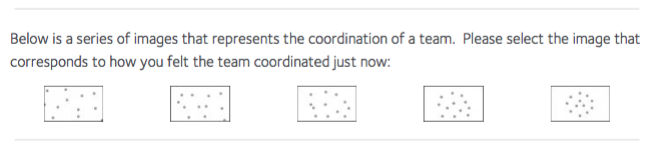
\includegraphics[width = \linewidth]{images/teamClickPictorial.png}
  \caption{Click Pictorial Scale}
  \label{fig:clickPictorial}
\end{figure}




    \subsubsection{Social Bonding}
In the pre- and post-Tournament surveys, social bonding was measured using the following items:
\begin{description}
  \item [Emotional Support] ``How emotionally supportive does the team feel?''
  \item [Shared Goal] ``How strong is the feeling that everyone is working towards a shared goal?''
  \item [Group Identification Verbal] A six-item scale designed to measure an individual's personal identification with the stereotypical features of the in-group  \citep{Mael1992}.  All 6 items were measured using a 5-point Likert scale.

%1. When someone critizes my team, it feels like a personal insult
%2. I am very interested in what others think about my team
%3. When I talk about my team, I usually say “we” rather than “they"
%4. This team's successes are my successes
%5. When someone praises my team, it feels like a personal compliment
%6. If a story in the media criticized my team, I would feel embarrassed

\item [Identity Fusion Verbal] A seven-item scale designed to measure an individual's ``feeling of oneness with the group'' \citep{Swann2009}.  Identity Fusion is differentiated from Group Identification in its ability to account for an individual's felt, emotional and personal agentic associations with being a member of the target in-group \citep{Swann2012a}.  All 7 items were measured using a 5-point Likert scale.

%1. I am one with my team.
%2. I feel immersed in my team.
%3. I have a deep emotional bond with my team.
%4. My team is me.
%5. I’ll do for my team more than any of the other team members would do.
%6. I am strong because of my team.
%7. I make my team strong.

\item [Identity Fusion Pictorial] A visual scale designed to measure Identity Fusion to the target in-group \citep{Swann2009}. The pictorial scale depicts two circles, one smaller circle to denote the individual, and one larger circle to denote the group, progressively moving closer to each other such that the most ``fused'' option depicts the smaller circle encased by the larger circle. The scale offers a total of five options to chose from, see Figure ~\ref{fig:fusionPictorialGroup}.  A total of three pictorial scales were included, each with different target in-groups: team, family, and country (China).
\item [Fusion Pictorial Rank] Athletes were asked to rank their fusion to team, family, and country \citep{Whitehouse2014}.  ``Thinking about these relationships [to team, family, and country] please rank them below in order of which you feel most connected to. 1 for most connected, 3 for least connected.''
\end{description}




\begin{figure}[htbp]
  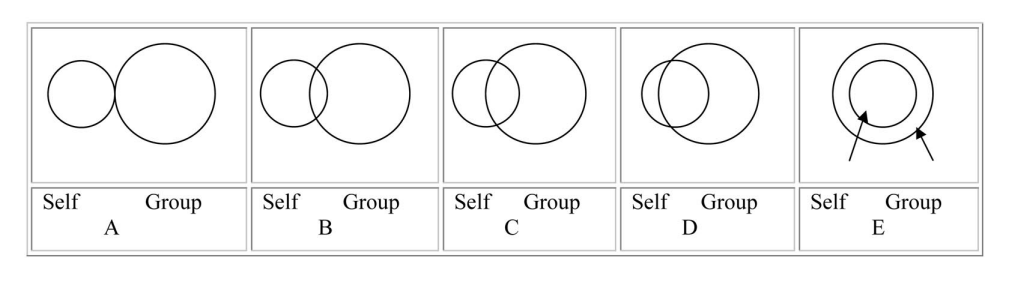
\includegraphics[width=\linewidth]{images/Identity_Fusion_Pictorial_Scale.png}
  \caption{Identity Fusion Pictorial Scale}
  \label{fig:fusionPictorialGroup}
\end{figure}

%\insert{../images/Identity_Fusion_Pictorial_Scale.png}.

\subsubsection{Exertion, Fatigue, and Injury}
Athletes were asked to report on various components of physical and mental fatigue, exertion, and injury.  Following each mid-Tournament survey and in the post-Tournament survey, athletes were asked about their mood (``How are you feeling now after the tournament?'') and responded by choosing a point on a 10-point scale between three pairs of emotions (``Not aroused / highly aroused'',  ``Depressed/Relaxed'' and  ``Nervous/Excited'').\footnote{Many athletes experienced difficulty filling out this item in the survey, as such it was not included in the analysis} Athletes were also asked about feelings of fatigue ``How fatigued do you feel as a result of the game/tournament?'', perceived physical exertion (Borg RPE scale, \citep{Borg1990} and perceived mental exertion using two 15-point scales \citep[see][ ]{Noakes2012a}.  Athletes were also asked to indicate their injury status on a 100-point scale (0 = ``Unable to play'', 100 = ``Completely fit to play'').  A baseline measure of injury was  collected in the pre-Tournament survey, but fatigue, exertion, and mood measures were not included in the pre-Tournament survey because of inappropriateness for the pre-Tournament context.





%        4.2.7
\subsubsection{Personality}
Due to the hypothesised links between personality type and dispositional tendencies towards interpersonal coordination strategies \citep{Marsh2009}, a ten-item personality measure was included in the pre-Tournament survey (Ten Item Personality Index - TIPI)\citep{Gosling2003}. Athletes were asked to indicate on a 7-point Likert scale the extent to which they agreed with 10 pairs of adjectives as appropriate descriptions of their personality (For example: ``I see myself as: dependable, self-disciplined''). In the TIPI, two items corresponded to each of the big-five personality types:

\begin{description}
\item [Extraversion:] 1. Extraverted, enthusiastic; 6. Reserved, quiet (Reversed scale)
\item [Agreeableness:] 2. Critical, quarrelsome (Reversed); 7. Sympathetic, warm
\item [Conscientiousness:] 3. Dependable, self-disciplined; 8. Disorganised, careless (Reversed)
\item [Emotional Stability:] 4. Anxious, easily upset (Reversed); 9. Calm, emotionally stable.
\item [Openness to Experiences:] 5. Open to new experiences, complex; 10.Conventional, uncreative (Reversed)
\end{description}







\subsection{Performance data and video data}
Following the completion of the Tournament, CRFA provided performance data in electronic format. These data included results for each game, minutes played and points scored by individual athletes in each game, substitutions made during each game, and video footage of every game played during the tournament. Data were stored on an encrypted external hard disk. \\

The following variables were created from the objective performance data for use as statistical controls in inferential analysis:

\begin{description}
\item [Final Rank:] A rank was given to each team based on performance in their respective competition (men's   women's). These rank scores were then reversed for the purposes of statistical analysis (1st place in men's Tournament (8 teams) = 8, 2nd place = 7, and so on)
\item [Total Wins - Losses:] A team's total number of losses was subtracted from its total number of wins.  Thus, more successful teams overall had a higher score.
\item [Total Minutes:] Total number of minutes played throughout the Tournament by each individual athlete
\item [Total Points:] Total number of points scored throughout the Tournament by each individual athlete
\item [Starting Team Average] An average measure indicating likelihood of an athlete being selected in the starting team. Each Athlete was awarded 1 point for each game he or she started in the starting team; reserve squad athletes were awarded zero for each game. Each athlete's total was divided by the total number of games that they participated in during the Tournament, including games in which they didn't take the field, to produce an average score for the Tournament.
\end{description}



























\clearpage
\section{Analysis}


\subsection{Overview of Analysis}

Predictions of this study were tested by analysing the collected data in three steps:

\begin{enumerate}
  \item A focussed analysis of the \textbf{post-Tournament} survey responses
  \item An analysis of \textit{changes} in variables between \textbf{pre- and post-Tournament} responses
  \item Analysis of the relationship between team performance, team click, and social bonding in survey data over the \textbf{entire Tournament}. \textit{Note that these data are still under analysis and will not be presented for assessment here.}
\end{enumerate}

Analysis of data collected following the Tournament (phase 1) provided an indication of the effects of a high-intensity, high stakes professional Tournament. Was there a statistically meaningful relationship between perceived team performance, team click, and social bonding in response to athlete experience of the Tournament?  Investigating the extent to which athlete responses varied across the Tournament provided a finer-grained picture of within-participation changes in associations among variables.  Can pre- to post-Tournament changes in outcome variables (team click, social bonding, and fatigue) be explained by pre-post Tournament variation in perceptions of joint-action success and feelings of team click?  Analysis of the entire survey data set, including pre-, mid-, and post-Tournament survey responses, allowed for a more thorough assessment of the consistency of a hypothesised relationship between joint-action success, team click, and social bonding. By analysing multiple observations for the same athlete over a number of time points, it was possible to better account for intra- and inter-individual variation, enabling more robust inferences.











\subsection{Analysis of post-Tournament data}
%\subsubsection{Roadmap of post-Tournament Analysis}
Analysis of the post-Tournament data proceeded by testing predictions associated with the overarching hypothesis, that higher perceptions of joint-action success would lead to higher levels of social bonding, mediated by feelings of ``team click''.

The first step was to assess whether the two variables hypothesised to be relevant to perceived joint-action success, 1) perceptions of team performance (Joint Action Success) and 2) appraisal of team performance relative to prior expectations (Team Performance Expectations), predicted feelings of team click (Team Click). Controlling for athlete perceptions of individual performance success, subjective and objective technical competence, Tournament performance measures, and variation attributable to team membership (random effect), linear mixed-effect regression models were used to test the following predictions:

\begin{description}
  \item [Prediction 1.a] Joint Action Success  $\rightarrow$ Team Click
  \item [Prediction 1.b] Team Performance Expectations $\rightarrow$ Team Click
  \item [Prediction 1.c] Joint Action Success $\rightarrow$ Team Click, moderated by Team Performance Expectations
\end{description}

Next, the relationship between team click (Team Click) and social bonding (Social Bonding) was tested, controlling for subjective and objective technical competence, Tournament performance measures, and variation attributable to team membership (random effect):

\begin{description}
  \item [Prediction 2.a] Team Click $\rightarrow$ Social Bonding
\end{description}

Following this, the direct relationships between two predictor variables of interest (Joint Action Success and Team Performance Expectations) and social bonding was tested:

\begin{description}
  \item [Prediction 3.a] Joint Action Success $\rightarrow$ Social Bonding
  \item [Prediction 3.b] Team Performance Expectations $\rightarrow$ Social Bonding
\end{description}

Finally, a mediation analysis was performed to formally test whether feelings of team click mediated a direct relationship between perceptions of joint-action success and social bonding.

\begin{description}
\item[Prediction 4.a Mediation Analysis] Joint Action Success $\rightarrow$ Team Click $\rightarrow$ Social Bonding
\item[Prediction 4.b Mediation Analysis] Team Performance Expectations $\rightarrow$ Team Click $\rightarrow$ Social Bonding
\end{description}











\subsubsection{post-Tournament Data}

118 (male = 65) out of a total of 174 athletes who participated in the Tournament completed the post-Tournament survey. Athletes completing the pre- and post-Tournament surveys were not subject to time constraints, and so the full complement of survey items for each category of variables outlined in the methods section (performance, click, bonding, and fatigue) were included. In addition to these survey responses, Tournament performance measures provided by CRFA, and measures of technical competence and other identification variables (age, sex, team affiliation, and so on) provided in the pre-Tournament survey were used to supplement analysis of the post-Tournament data. Summary statistics for each category of survey variables are outlined in Tables below.

\begin{table}[htpb]\caption{Summary Statistics: post-Tournament Technical Competence (objective and subjective)}
\begin{center}
\begin{small} 
\begin{tabular}
{l
r
r
r
r
r
r
r
}

\multicolumn{
7
}{l}{

}
\cr 
 \hline 
Variable  &  
n  & 
mean  & 
sd  & 
min  & 
max  & 
skew  & 
krtss \cr 

 \hline 

Years In Team   &  120  &   3.17  &   2.12  &    0  &   7  &   0.29  &  -1.25 \cr 

Training Age   &  120  &   4.40  &   2.35  &    0  &  13  &   0.47  &   0.66 \cr 

Starting Team Average   &  172  &   0.61  &   0.36  &    0  &   1  &  -0.43  &  -1.32 \cr 

Age   &  121  &  21.67  &   3.26  &   16  &  32  &   0.52  &  -0.27 \cr 

Ability Teammates   &  120  &  19.45  &  20.14  &  -40  &  50  &  -0.31  &  -0.56 \cr 

Ability Chinese Pros   &  120  &  15.78  &  19.59  &  -35  &  50  &  -0.18  &  -0.65 \cr 

Ability International   &  120  &  18.46  &  26.19  &  -44  &  50  &  -0.48  &  -0.77 \cr 

Team Ability China   &  120  &  22.48  &  22.90  &  -40  &  50  &  -0.64  &  -0.58 \cr 

 \hline 
\end{tabular}
\end{small}
\end{center}
\label{tab:1competenceDescriptives}
\end{table} 



\begin{table}[htpb]\caption{Summary Statistics: post-Tournament Performance (individual and team)}
\begin{center}
\begin{small} 
\begin{tabular}
{l
r
r
r
r
r
r
r
}

\multicolumn{
7
}{l}{

}
\cr 
 \hline 
Variable  &  
{n} & 
{mean} & 
{sd} & 
{min} & 
{max} & 
{skew} & 
{krtss}\cr 

 \hline 

indPerformance7   &  118  &  56.36  &  23.47  &  0  &  100  &  -0.35  &  -0.08 \cr 

passingTech7   &  118  &  58.41  &  24.25  &  0  &  100  &  -0.79  &   0.05 \cr 

supportAttack7   &  118  &  62.62  &  22.70  &  0  &  100  &  -0.98  &   0.64 \cr 

indDefense7   &  118  &  57.64  &  23.57  &  0  &  100  &  -0.55  &  -0.11 \cr 

effectContact7   &  118  &  62.15  &  24.81  &  0  &  100  &  -0.97  &   0.40 \cr 

decisionAttack7   &  118  &  61.22  &  21.43  &  0  &  100  &  -0.72  &   0.37 \cr 

teamPerformance7   &  118  &  64.36  &  23.61  &  0  &  100  &  -0.52  &  -0.30 \cr 

teamDefense7   &  118  &  62.42  &  22.50  &  0  &  100  &  -0.52  &  -0.52 \cr 

teamAttack7   &  118  &  65.33  &  20.26  &  0  &  100  &  -0.53  &  -0.23 \cr 

teamSupportPlay7   &  118  &  65.75  &  19.72  &  0  &  100  &  -0.76  &   0.57 \cr 

teamCommunication7   &  118  &  65.25  &  21.26  &  0  &  100  &  -0.65  &   0.27 \cr 

 \hline 
\end{tabular}
\end{small}
\end{center}
\label{tab:2performancePostDescriptives}
\end{table} 



\begin{table}[htpb]\caption{Summary Statistics: post-Tournament Team Click}
\begin{center}
\begin{small} 
\begin{tabular}
{l
r
r
r
r
r
r
r
}

\multicolumn{
7
}{l}{

}
\cr 
 \hline 
Variable  &  
{n} & 
{mean} & 
{sd} & 
{min} & 
{max} & 
{skew} & 
{krtss}\cr 

 \hline 

unspokenUnderstanding7   &  118  &  72.72  &  19.95  &  0  &  100  &  -1.38  &  2.13 \cr 

generalAtmosphere7   &  118  &  78.45  &  21.34  &  0  &  100  &  -1.51  &  2.82 \cr 

clickPictorial7   &  118  &   3.93  &   1.04  &  1  &    5  &  -0.78  &  0.00 \cr 

reliabilityOfOthers7   &  118  &  68.00  &  23.09  &  0  &  100  &  -1.33  &  1.75 \cr 

reliabilityForOthers7   &  118  &  63.45  &  25.80  &  0  &  100  &  -1.06  &  0.51 \cr 

abilityExtended7   &  118  &  72.25  &  19.27  &  0  &  100  &  -1.13  &  2.03 \cr 

 \hline 
\end{tabular}
\end{small}
\end{center}
\label{tab:3clickPostDescriptives}
\end{table} 



\begin{table}[htpb]\caption{Summary Statistics: post-Tournament Social Bonding}
\begin{center}
\begin{small} 
\begin{tabular}
{l
r
r
r
r
r
r
r
}

\multicolumn{
7
}{l}{

}
\cr 
 \hline 
Variable  &  
{n} & 
{mean} & 
{sd} & 
{min} & 
{max} & 
{skew} & 
{krtss}\cr 

 \hline 

emotionalSupport7   &  118  &  79.67  &  18.84  &   0.00  &  100  &  -1.74  &  4.37 \cr 

sharedGoal7   &  118  &  86.00  &  15.56  &  29.00  &  100  &  -1.38  &  2.24 \cr 

groupId7   &  118  &   4.29  &   0.67  &   1.50  &    5  &  -1.18  &  1.66 \cr 

fusionVerbal7   &  118  &   4.00  &   0.71  &   1.43  &    5  &  -0.86  &  0.99 \cr 

fusionPictorialTeam7   &  118  &   4.33  &   1.19  &   0.00  &    5  &  -2.45  &  6.07 \cr 

fusionPictorialFamily7   &  118  &   4.51  &   0.96  &   0.00  &    5  &  -2.30  &  5.62 \cr 

fusionPictorialCountry7   &  118  &   4.03  &   1.39  &   0.00  &    5  &  -1.59  &  1.84 \cr 

 \hline 
\end{tabular}
\end{small}
\end{center}
\label{tab:4bondingPostDescriptives}
\end{table} 



\begin{table}[htpb]\caption{Summary Statistics: post-Tournament measures of fatigue}
\begin{center}
\begin{small} 
\begin{tabular}
{l
r
r
r
r
r
r
r
}

\multicolumn{
7
}{l}{

}
\cr 
 \hline 
Variable  &  
n  & 
mean  & 
sd  & 
min  & 
max  & 
skew  & 
krtss \cr 

 \hline 

Fatigue   &  118  &  69.27  &  21.24  &   0  &  100  &  -1.13  &  1.40 \cr 

RPE(physical)   &  118  &  14.97  &   2.66  &   6  &   20  &  -0.80  &  0.49 \cr 

RPE(mental)   &  118  &   6.08  &   2.47  &  -4  &   10  &  -1.13  &  1.82 \cr 

injuryRev7   &  118  &  23.86  &  26.91  &   0  &  100  &   1.19  &  0.60 \cr 

 \hline 
\end{tabular}
\end{small}
\end{center}
\label{tab:5fatiguePostDescriptives}
\end{table} 



\begin{table}[htpb]\caption{Summary Statistics: Objective Tournament Performance}
\begin{center}
\begin{small} 
\begin{tabular}
{l
r
r
r
r
r
r
r
}

\multicolumn{
7
}{l}{

}
\cr 
 \hline 
Variable  &  
n  & 
mean  & 
sd  & 
min  & 
max  & 
skew  & 
krtss \cr 

 \hline 

Final Rank   &  174  &   4.83  &   2.15  &   1  &   8  &  -0.09  &  -1.17 \cr 

Wins - Losses   &  172  &   0.32  &   2.94  &  -6  &   6  &  -0.17  &  -0.25 \cr 

Total Ind Points   &  172  &   8.45  &  11.41  &   0  &  69  &   2.34  &   7.23 \cr 

Total Ind Minutes   &  172  &  44.01  &  20.65  &   1  &  81  &  -0.38  &  -0.89 \cr 

Starting Team Avg   &  172  &   0.61  &   0.36  &   0  &   1  &  -0.43  &  -1.32 \cr 

 \hline 
\end{tabular}
\end{small}
\end{center}
\label{tab:6objectiveTournamentDescriptives}
\end{table} 




Table ~\ref{tab:1competenceDescriptives} displays the variables relevant to an Athlete's technical competence.  These variables were collected in the pre-Tournament survey, and as such the number of observations per variable is generally 120, except for ``Starting Team Average,'' which was generated from the objective performance data provided by CRFA following the Tournament.  The average number of years in the team was over three years, and the average training age for Athletes was 4.4 years.  In terms of subjective confidence, means for each variable were well above the mid-point of the scale, suggesting that Athletes were on average quite positive about their own ability compared to other athletes (their teammates, other Chinese professionals, International professionals).  Table ~\ref{tab:2performancePostDescriptives} also shows that athletes on average rated their individual and team performance above the mid-point of the scale, with team performance variables appearing slightly higher that individual performance variables.  As Table ~\ref{tab:3clickPostDescriptives} indicates, this trend was even more pronounced for variables relating to team click, with the central tendency for each variable ranging between 65 and 78 (100-point scale, SD range =  19-27). The exception to this was the 5-point pictorial click variable, the average for which was 3.93 (out of 5, SD = 1.04).  All six items relating to click had a pronounced negative skew.  As Table ~\ref{tab:4bondingPostDescriptives} demonstrates, the trend for bonding was even higher, with central tendencies for Emotional Support and Shared Goal 79.67 (SD = 18.84) and 86 (SD = 15.56) respectively.  All five-point Likert scales also had an extremely negatively skewed distribution, with central tendencies between 4 (Identity Fusion Verbal, SD = .71) and 4.51 (Identity Fusion Family, SD = 0.96).  Table ~\ref{tab:5fatiguePostDescriptives} indicates that, in regards to fatigue variables, Athletes also scored on average above the mid-point of the scale for each item.  In regards to Objective Tournament Performance (~\ref{tab:6objectiveTournamentDescriptives}), Athletes played an average of 44 minutes of rugby during the Tournament (just under four full games each), and each Athlete scored an average of 8.45 points, which amounts to between one and two tries each, or a number of try drop-kick conversions (worth two points each).



\clearpage







\subsubsection{Data Reduction} \label{subsection:dataReduction}
Data reduction was required in order to make analysis of predicted relationships more tractable and parsimonious. Data reduction allows for a reduction in multicolinearity between predictor variables of interest while retaining as much variance as possible in the observed data \citep{Yong2013}.  Given that the survey items of this study were designed to collectively access more latent psychological constructs, particularly in the case of outcome variables related to concepts such as team click, social bonding, and fatigue (but also for performance variables), a data reduction technique capable of modelling the theoretical structure of these data was preferred.  Exploratory Factor Analysis (EFA) was thus chosen as the most suitable data reduction technique (for a full explanation of EFA, see appendix ~\ref{section:EFA}).

EFA was performed on key variables of interest, including team component performance (jointActionSuccess), individual component performance (indPerformanceComponents), teamClick, socialBonding, fatigue, and technicalCompetence (objective and subjective). Perceptions of team and individual performance relative to prior expectations were both single-item measures and thus did not require data reduction.  Prior to factors being extracted, correlation matrices were subjected to two common sampling adequacy measures: the Kaiser-Meyer-Olkin (KMO) index and Bartlett’s test of sphericity. The KMO index provides a proportion measure of common variance to partial correlations among examined variables\footnote{If the KMO index is high ($\approx$ 1), the EFA can act efficiently; if KMO is low ($\approx$ 0), the proposed EFA is not suitable for analysis.} while Bartlett’s test of sphericity is used to test the null hypothesis that the correlation matrix is an identity matrix (i.e., a square matrix in which all the elements of the principal diagonal are equal to 1, and all other elements are 0s). Factor loadings of $> .3$ were considered adequate, and only items that loaded on one factor were accepted \citep{Field2012}. Finally, two reliability measures (Guttman's lambda3 and Cronbach's Alpha) were also reported as an indication of whether or not the average correlation of each subset of variables is an accurate estimate of the average correlation of all items that could pertain to the underlying construct.\footnote{Cronbach's $\alpha$ is a function of the number of items in a test, the average covariance between item-pairs, and the variance of the total score \citep{Tabachnick2007}} Eigenvalues, or Sum of Squares Loadings (SS Loadings) for each factor were also reported\citep{Dziuban1974}.

\subsubsection{EFA of post-Tournament Variables}

\myparagraph{Component Performance for Individual and Team}
Items related to athlete perception of components of performance were isolated from overall perceptions of performance relative to prior individual expectations for further data reduction. Given that the theoretical predictions of this dissertation concentrate in particular on athlete perceptions of joint-action, individual and team components of performance were analysed separately. This separation allows for the testing the differential effects of perceptions of individual and team performance on team click and social bonding. In addition, perceptions of success in individual performance components could be used as a statistical control for perceptions of joint-action success.

Items concerning team component performance (team defence, team attack, team support play, and on field communication) were subjected to EFA (with oblique ``promax'' rotation).  Correlations between team component performance items was very high (all $r's > .5$), which suggested that one factor would be appropriate (see Table ~\ref{tab:22teamPerformancePostCorr}). The KMO index and Bartlett's test both suggested high sampling adequacy, ($KMO = 0.79$, $\chi^2(6, N = 118) = 342.14$, $p < .001$).  One factor, labelled ``Joint Action Success'' was imposed on the data, which explained 72.8\% of the overall variance (SS Loading = 2.91). $Guttman's \lambda =.90$ and $Cronbach's \alpha = .91$ indicated that the data reduction was appropriate and reliable.

%, $\chi^2 (df=2) = 14.81$, $p < .001$,

Items relating to individual component performance (passing technique, support play in attack, 1on1 defence, and decision making in attack) were subjected to an EFA.  Correlations between individual component performance items were also very high (all $r's > .5$, see Table ~\ref{tab:21indPerformancePostCorr}), which suggested that one factor would be sufficient (confirmed by $KMO =  0.84$, corrtest Bartlett: $\chi^2(10, N = 118) =  326.38$, $p < .001$).  One factor was extracted and labelled ``Ind Performance Success'', which explained 62.1\% of the overall variance (SS Loading = 3.10) .  $Guttman's \lambda =.88$ and $Cronbach's \alpha = .89$ both indicated that the data reduction was appropriate.
%$\chi^2 (df=5) = 15.47$, $p < .01$

To confirm that the theoretically motivated separation of Joint Action Success from Ind Performance Success was appropriate for the collected data, a follow up EFA was conducted, in which team and individual performance component variables were combined in one matrix. Sampling adequacy measures indicated high suitability ($KMO = 0.83$, $\chi^2(36, N = 118) = 726.60$, $p < .0001$).  As expected, an EFA extracted two factors, with Individual performance measures loaded on one factor (proportion of variance = .34, $SS Loading = 3.09$), and team performance measures loading on a second factor (proportion of variance = .32, $SS Loading = 2.90$). $Guttman's \lambda =.93$ and $Cronbach's \alpha = .90$ indicated that the data reduction was appropriate.


\myparagraph{Team Click}
EFA was performed on post-Tournament variables associated with team click. Strong correlations between all variables of interest ($r's > .3$, see Table ~\ref{tab:3clickPostCorr}) and sampling adequacy measures suggested that imposing one factor was appropriate, $KMO =  0.69$, $\chi^2(15, N = 118) = 182.73$, $p < .001$.  One factor labelled ``Team Click'' was extracted from the data, which explained 34.5\% of the overall variance ($SS Loading = 2.07$).  Guttman's $\lambda =.76$ and Cronbach's $\alpha = .75$ indicated that the data reduction was appropriate.  These reliability statistics provided confidence that the novel pictorial click measure related strongly to the ethnogrpahically derived click items (for example, Unspoken Understanding and General Atmostphere).
%, and a Chi-squared test indicated that one factor was sufficient to account for the variance of these items ($\chi^2 (9, ) = 46.36$, $p < .001$).

%Interestingly, when click and bonding measures were analysed together, the following loading were observed:
%Loadings:
%                       Factor1 Factor2
%unspokenUnderstanding7  0.710
%generalAtmosphere7      0.713
%clickPictorial7         0.672  -0.106
%reliabilityOfOthers7    0.128   0.539
%reliabilityForOthers7           0.424
%abilityExtended7       -0.110   0.956
%emotionalSupport7       0.656   0.131
%sharedGoal7             0.838
%fusionPictorialTeam7    0.424
%fusionVerbal7           0.138   0.281


\myparagraph{Social Bonding}
Survey items related to feelings of social bonding (within the team) were separately analysed for the purposes of data reduction. A correlation matrix (~\ref{tab:4bondingPostCorr}) indicated that Group Identification did not share common variance with other variables (all correlations were $<.1$, except for the verbal measures of Identity Fusion ($r =.358$)). As such,  Group Identification was excluded from analysis.  Sampling adequacy variables suggested that the remaining subset of variables were appropriate for analysis, $KMO = 0.65$, $\chi^2(10, N = 118) = 108.22$, $p < .001$.  EFA was performed on 4 remaining items, imposing one factor labelled ``Social Bonding'', which explained 34.5\% of the overall variance ($SS Loading = 1.60$, $Guttman's \lambda =.66$ and $Cronbach's \alpha = .65$).

\myparagraph{Fatigue}
Finally, post-Tournament survey items relating to perceptions of fatigue and exertion were separately analysed for the purposes of data reduction.  Due to difficulty completing questions related to arousal in the online and in-person surveys, mood-related items were excluded from analysis.  In addition, it was clear from correlation values that injury status did not strongly correlate with other items relevant to fatigue and exertion, and was therefore also excluded from subsequent analysis (see Table ~\ref{tab:5fatiguePostCorr}).  The KMO index and Bartlett's test of sphericity indicated that the remaining subset of variables was appropriate for EFA, $KMO =  0.69$, $\chi^2(3, N = 118) = 111.93$, $p < .001$. EFA was performed on 3 remaining items (fatigue, physical perceived exertion, and mental perceived exertion), which imposed one factor labelled ``Fatigue Factor.''  The extracted factor explained 57.8\% of the overall variance (SS Loadings = 1.7, $Guttman's\lambda =.73$ and Cronbach's $\alpha = .80$).

\myparagraph{Technical Competence}
All eight items relevant to technical competence were analysed in a correlation matrix to assess relatedness (see Table ~\ref{tab:1competenceCorr}). Medium correlations among measures of objective competence (three out of four items correlated at $> .3$) and among measures of subjective competence (all items except for team competence measure correlated at $> .3$) suggested that the data could be explained by two underlying factors. Team Ability Chinese Provinces was dropped from analysis due to low correlation with other competence variables, possibly because the item did not ask about an individual athlete’s competence (it referred instead to an athlete’s opinion of the competence of the team of which they were a member). An examination of the KMO measure of sampling adequacy ($KMO = .67$), and the Bartlett sphericity test indicated that two factors were adequate, $\chi^2(21, N = 120) = 239.71$, $p < .001$. \\

An EFA of technical competence variables revealed that items of interest loaded on two factors. The exception was the variable Starting Reserve, which failed to load on either factor, and was thus dropped from analysis. Measures of objective competence (Years Team, Training Age, and Age) loaded on the first factor, which was labelled ``Objective Competence'' because the measures were all objective markers of an athlete's competence.  Objective Competence explained 26.4\% of the total variance ($SS Loading = 1.85$). The remaining measures of subjective competence (Ability Teammates, Ability Chinese Pros, Ability International Pros) loaded on the remaining factor.  The second factor was labelled ``Subjective Competence'', due to the fact that all measures were the product of athlete self-report.  Subjective competence explained 23.8\% of the variance ($SS Loading = 1.67$). $Guttman's \lambda =.74$ and $Cronbach's \alpha = (.67)$ indicated that the data reduction was appropriate and reliable.











Summary statistics for the factors extracted from the post-Tournament data, and their correlations can be viewed in Table ~\ref{tab:postTournamentFactorDescriptives} and Table ~\ref{tab:postTournamentFactorCorr} respectively.

\newpage
\newgeometry{margin=0.5cm} % modify this if you need even more space
\begin{landscape}


% Table created by stargazer v.5.2.2 by Marek Hlavac, Harvard University. E-mail: hlavac at fas.harvard.edu
% Date and time: Mon, Aug 27, 2018 - 18:51:00
\begin{table}[!htbp] \centering 
  \caption{Correlation Matrix: post-Tournament Technical Competence} 
  \label{tab:1competenceCorr} 
\scriptsize 
\begin{tabular}{@{\extracolsep{5pt}} ccccccccc} 
\\[-1.8ex]\hline 
\hline \\[-1.8ex] 
 & Years In Team & Training Age & Starting Team Average & Age & Ability Teammates & Ability Chinese Pros & Ability International & Team Ability China \\ 
\hline \\[-1.8ex] 
Years In Team & $1$ & $0.510$ & $$-$0.044$ & $0.569$ & $0.076$ & $0.102$ & $0.099$ & $0.261$ \\ 
Training Age & $0.510$ & $1$ & $0.0004$ & $0.697$ & $0.095$ & $0.183$ & $0.201$ & $0.190$ \\ 
Starting Team Average & $$-$0.044$ & $0.0004$ & $1$ & $$-$0.040$ & $0.203$ & $0.099$ & $0.044$ & $0.144$ \\ 
Age & $0.569$ & $0.697$ & $$-$0.040$ & $1$ & $0.132$ & $0.089$ & $0.154$ & $0.212$ \\ 
Ability Teammates & $0.076$ & $0.095$ & $0.203$ & $0.132$ & $1$ & $0.428$ & $0.383$ & $0.454$ \\ 
Ability Chinese Pros & $0.102$ & $0.183$ & $0.099$ & $0.089$ & $0.428$ & $1$ & $0.702$ & $0.273$ \\ 
Ability International & $0.099$ & $0.201$ & $0.044$ & $0.154$ & $0.383$ & $0.702$ & $1$ & $0.212$ \\ 
Team Ability China & $0.261$ & $0.190$ & $0.144$ & $0.212$ & $0.454$ & $0.273$ & $0.212$ & $1$ \\ 
\hline \\[-1.8ex] 
\end{tabular} 
\end{table} 


% Table created by stargazer v.5.2 by Marek Hlavac, Harvard University. E-mail: hlavac at fas.harvard.edu
% Date and time: Sun, Jun 25, 2017 - 21:08:16
\begin{table}[!htbp] \centering 
  \caption{Correlation Matrix: post-Tournament Team Performance} 
  \label{tab:22teamPerformancePostCorr} 
\footnotesize 
\begin{tabular}{@{\extracolsep{5pt}} ccccc} 
\\[-1.8ex]\hline 
\hline \\[-1.8ex] 
 & Team Defence & Team Attack & Team Support Play & Team Onfield Communication \\ 
\hline \\[-1.8ex] 
Team Defence & $1$ & $0.834$ & $0.643$ & $0.721$ \\ 
Team Attack & $0.834$ & $1$ & $0.740$ & $0.713$ \\ 
Team Support Play & $0.643$ & $0.740$ & $1$ & $0.715$ \\ 
Team Onfield Communication & $0.721$ & $0.713$ & $0.715$ & $1$ \\ 
\hline \\[-1.8ex] 
\end{tabular} 
\end{table} 


% Table created by stargazer v.5.2 by Marek Hlavac, Harvard University. E-mail: hlavac at fas.harvard.edu
% Date and time: Sun, Jun 25, 2017 - 21:07:58
\begin{table}[!htbp] \centering 
  \caption{Correlation Matrix: Individual Performance} 
  \label{tab:21indPerformancePostCorr} 
\footnotesize 
\begin{tabular}{@{\extracolsep{5pt}} cccccc} 
\\[-1.8ex]\hline 
\hline \\[-1.8ex] 
 & Passing Tech & Support In Attack & Ind Defence & Effectiveness In Contact & Decision Making Attack \\ 
\hline \\[-1.8ex] 
Passing Tech & $1$ & $0.658$ & $0.510$ & $0.508$ & $0.607$ \\ 
Support In Attack & $0.658$ & $1$ & $0.658$ & $0.641$ & $0.734$ \\ 
Ind Defence & $0.510$ & $0.658$ & $1$ & $0.590$ & $0.525$ \\ 
Effectiveness In Contact & $0.508$ & $0.641$ & $0.590$ & $1$ & $0.713$ \\ 
Decision Making Attack & $0.607$ & $0.734$ & $0.525$ & $0.713$ & $1$ \\ 
\hline \\[-1.8ex] 
\end{tabular} 
\end{table} 


% Table created by stargazer v.5.2.2 by Marek Hlavac, Harvard University. E-mail: hlavac at fas.harvard.edu
% Date and time: Mon, Aug 27, 2018 - 18:51:00
\begin{table}[!htbp] \centering 
  \caption{Correlation Matrix: post-Tournament Team Click} 
  \label{} 
\footnotesize 
\begin{tabular}{@{\extracolsep{5pt}} ccccccc} 
\\[-1.8ex]\hline 
\hline \\[-1.8ex] 
 & unspokenUnderstanding7 & generalAtmosphere7 & clickPictorial7 & reliabilityOfOthers7 & reliabilityForOthers7 & abilityExtended7 \\ 
\hline \\[-1.8ex] 
unspokenUnderstanding7 & $1$ & $0.626$ & $0.508$ & $0.275$ & $0.230$ & $0.375$ \\ 
generalAtmosphere7 & $0.626$ & $1$ & $0.385$ & $0.301$ & $0.276$ & $0.265$ \\ 
clickPictorial7 & $0.508$ & $0.385$ & $1$ & $0.282$ & $0.021$ & $0.213$ \\ 
reliabilityOfOthers7 & $0.275$ & $0.301$ & $0.282$ & $1$ & $0.276$ & $0.544$ \\ 
reliabilityForOthers7 & $0.230$ & $0.276$ & $0.021$ & $0.276$ & $1$ & $0.375$ \\ 
abilityExtended7 & $0.375$ & $0.265$ & $0.213$ & $0.544$ & $0.375$ & $1$ \\ 
\hline \\[-1.8ex] 
\end{tabular} 
\end{table} 


\clearpage

% Table created by stargazer v.5.2 by Marek Hlavac, Harvard University. E-mail: hlavac at fas.harvard.edu
% Date and time: Tue, May 30, 2017 - 09:19:43
\begin{table}[!htbp] \centering 
  \caption{Correlation Matrix: post-Tournament Social Bonding} 
  \label{} 
\footnotesize 
\begin{tabular}{@{\extracolsep{5pt}} cccccc} 
\\[-1.8ex]\hline 
\hline \\[-1.8ex] 
 & emotionalSupport & sharedGoal & groupIdentification & identityFusionVerbal & identityFusionPictorialTeam \\ 
\hline \\[-1.8ex] 
emotionalSupport & $1$ & $0.619$ & $0.079$ & $0.331$ & $0.349$ \\ 
sharedGoal & $0.619$ & $1$ & $0.061$ & $0.246$ & $0.395$ \\ 
groupIdentification & $0.079$ & $0.061$ & $1$ & $0.358$ & $0.081$ \\ 
identityFusionVerbal & $0.331$ & $0.246$ & $0.358$ & $1$ & $0.220$ \\ 
identityFusionPictorialTeam & $0.349$ & $0.395$ & $0.081$ & $0.220$ & $1$ \\ 
\hline \\[-1.8ex] 
\end{tabular} 
\end{table} 


% Table created by stargazer v.5.2 by Marek Hlavac, Harvard University. E-mail: hlavac at fas.harvard.edu
% Date and time: Sat, Jun 03, 2017 - 22:22:24
\begin{table}[!htbp] \centering 
  \caption{Correlation Matrix: post-Tournament Fatigue} 
  \label{} 
\footnotesize 
\begin{tabular}{@{\extracolsep{5pt}} ccccc} 
\\[-1.8ex]\hline 
\hline \\[-1.8ex] 
 & fatigue & RPE(physical) & RPE(mental) & injuryRev7 \\ 
\hline \\[-1.8ex] 
fatigue & $1$ & $0.665$ & $0.510$ & $0.090$ \\ 
RPE(physical) & $0.665$ & $1$ & $0.523$ & $0.009$ \\ 
RPE(mental) & $0.510$ & $0.523$ & $1$ & $$-$0.040$ \\ 
injuryRev7 & $0.090$ & $0.009$ & $$-$0.040$ & $1$ \\ 
\hline \\[-1.8ex] 
\end{tabular} 
\end{table} 


% Table created by stargazer v.5.2 by Marek Hlavac, Harvard University. E-mail: hlavac at fas.harvard.edu
% Date and time: Tue, May 30, 2017 - 09:19:44
\begin{table}[!htbp] \centering 
  \caption{Tournament Performance Correlation Matrix} 
  \label{} 
\footnotesize 
\begin{tabular}{@{\extracolsep{5pt}} cccccc} 
\\[-1.8ex]\hline 
\hline \\[-1.8ex] 
 & finalRank & totalWins - totalLosses & totalIndPoints & totalMinutesPlayed & startingTeamAvg \\ 
\hline \\[-1.8ex] 
finalRank & $1$ & $0.901$ & $0.381$ & $0.062$ & $0.055$ \\ 
totalWins - totalLosses & $0.901$ & $1$ & $0.428$ & $0.129$ & $0.089$ \\ 
totalIndPoints & $0.381$ & $0.428$ & $1$ & $0.404$ & $0.067$ \\ 
totalMinutesPlayed & $0.062$ & $0.129$ & $0.404$ & $1$ & $$-$0.038$ \\ 
startingTeamAvg & $0.055$ & $0.089$ & $0.067$ & $$-$0.038$ & $1$ \\ 
\hline \\[-1.8ex] 
\end{tabular} 
\end{table} 


\clearpage
\begin{table}[htpb]\caption{Summary Statistics: post-Tournament Factors}
\begin{center}
\begin{scriptsize} 
\begin{tabular}
{l
r
r
r
r
r
r
r
}

\multicolumn{
7
}{l}{

}
\cr 
 \hline 
Variable  &  
n  & 
mean  & 
sd  & 
min  & 
max  & 
skew  & 
krtss \cr 

 \hline 

objCompetence   &  120  &   0.00  &   0.95  &  -1.99  &    2.91  &   0.45  &  -0.23 \cr 

subjCompetence   &  120  &   0.00  &   0.96  &  -2.58  &    1.79  &  -0.16  &  -0.66 \cr 

indPerformExp   &  118  &  56.36  &  23.47  &   0.00  &  100.00  &  -0.35  &  -0.08 \cr 

indPerformSuccess   &  118  &   0.00  &   0.95  &  -2.96  &    1.70  &  -0.85  &   0.60 \cr 

teamPerformanceExpect   &  118  &  64.36  &  23.61  &   0.00  &  100.00  &  -0.52  &  -0.30 \cr 

jointActionSuccess   &  118  &   0.00  &   0.96  &  -3.28  &    1.79  &  -0.49  &  -0.01 \cr 

teamClick   &  118  &   0.00  &   0.90  &  -3.06  &    1.42  &  -1.01  &   1.03 \cr 

socialBonding   &  118  &   0.00  &   0.89  &  -3.08  &    1.08  &  -1.38  &   2.00 \cr 

fatigue   &  118  &   0.00  &   0.91  &  -3.40  &    1.67  &  -1.03  &   1.56 \cr 

 \hline 
\end{tabular}
\end{scriptsize}
\end{center}
\label{tab:postTournamentFactorDescriptives}
\end{table} 




% Table created by stargazer v.5.2.2 by Marek Hlavac, Harvard University. E-mail: hlavac at fas.harvard.edu
% Date and time: Mon, Aug 27, 2018 - 18:51:01
\begin{table}[!htbp] \centering 
  \caption{post-Tournament Factors Correlation Matrix} 
  \label{tab:postTournamentFactorCorr} 
\scriptsize 
\begin{tabular}{@{\extracolsep{5pt}} cccccccccc} 
\\[-1.8ex]\hline 
\hline \\[-1.8ex] 
 & objCompetence & subjCompetence & indPerformExp & indPerformSuccess & teamPerformanceExpect & jointActionSuccess & teamClick & socialBonding & fatigue \\ 
\hline \\[-1.8ex] 
objCompetence & $1$ & $$-$0.146$ & $0.065$ & $0.319$ & $$-$0.128$ & $$-$0.150$ & $0.011$ & $0.017$ & $0.084$ \\ 
subjCompetence & $$-$0.146$ & $1$ & $$-$0.086$ & $0.125$ & $$-$0.067$ & $0.044$ & $0.145$ & $0.195$ & $$-$0.045$ \\ 
indPerformExp & $0.065$ & $$-$0.086$ & $1$ & $0.411$ & $0.454$ & $0.285$ & $0.226$ & $0.180$ & $0.221$ \\ 
indPerformSuccess & $0.319$ & $0.125$ & $0.411$ & $1$ & $0.411$ & $0.490$ & $0.414$ & $0.273$ & $0.245$ \\ 
teamPerformanceExpect & $$-$0.128$ & $$-$0.067$ & $0.454$ & $0.411$ & $1$ & $0.709$ & $0.570$ & $0.314$ & $0.204$ \\ 
jointActionSuccess & $$-$0.150$ & $0.044$ & $0.285$ & $0.490$ & $0.709$ & $1$ & $0.686$ & $0.404$ & $0.202$ \\ 
teamClick & $0.011$ & $0.145$ & $0.226$ & $0.414$ & $0.570$ & $0.686$ & $1$ & $0.674$ & $0.271$ \\ 
socialBonding & $0.017$ & $0.195$ & $0.180$ & $0.273$ & $0.314$ & $0.404$ & $0.674$ & $1$ & $0.199$ \\ 
fatigue & $0.084$ & $$-$0.045$ & $0.221$ & $0.245$ & $0.204$ & $0.202$ & $0.271$ & $0.199$ & $1$ \\ 
\hline \\[-1.8ex] 
\end{tabular} 
\end{table} 



\end{landscape}
\restoregeometry





\subsubsection{Post-Tournament Data Structure}
The multilevel structure of the data (individual athletes nested within their respective teams; teams nested within the men’s and women’s competitions) suggests dependency in the data, or the possibility that residuals of observations for each grouping variables (team or sex) could be correlated. In addition, the data were unbalanced, meaning that there were an uneven number of observations recorded for each of the 15 teams. These particularities of the data posed challenges for analysis, due to the violation of the assumptions of independence and equality of variance.

\subsubsection{Intra-Class Correlation}
To assess the need for a statistical model capable of accounting for correlation of residuals, dependency in the data had to be quantified. A ratio measure comparing within- and between-group variance, known as the intra-class correlation (ICC), was calculated for each analysis to determine the extent to which athlete responses were clustered according to team or Tournament competition (i.e., sex). For team-level variance, a one-way random effects model was used, in which average within-team variance (Mean Square Within) of the response variable was divided by the average total variance of the response (Mean Square Total) \citep{Field2005a}.  Each athlete is member of one of 15 teams, which are considered to be sampled from a larger pool of potential teams, hence treated as random effects. The ICC is then interpreted as the percentage of total variance accounted for by group-level variables \citep{Wolak2012}.
To statistically account for the unbalanced design of the data, an adjusted sample-size coefficient (k) was calculated using an equation provided by \citep{Lessells1987}.  While there is no firm agreement on what is deemed meaningful within-group variance, an ICC ratio of $>.10-1.00$ with confidence intervals that do not include zero was considered a strong indication of non-random correlation of group-level residuals \citep{Bailey2011}. As Table ~\ref{tab:ICCsummaryTeam} and ~\ref{tab:ICCsummarySex} indicate, small to moderate team-level intra-class correlation of responses exist for factors of Objective Competence, Joint Action Success, Individual Performance Success, and Team Click. ICCs for Social Bonding and Fatigue meanwhile were relatively low (all $r's <.1$). Sex-level ICCs were all relatively low, suggesting that sex-level variation could be ignored in subsequent inferential analyses.\\


In addition to an assessment of ICC values, mean differences in variables of interest were assessed. Owing to the large number of grouping variables (team = 15), pairwise t-tests were not an appropriate way to compute team-level mean differences. Missing values in the data also meant that a standard ANOVA test was also not optimal for multiple group mean comparisons.  Instead, linear regressions were used to approximate differences between group-level responses for post-Tournament survey responses.  Team was used as the predictor variable, and factors derived from performance, click, social bonding, and fatigue variables were used as the outcome variables.  Analyses revealed:

\begin{itemize}
  \item Significant team-level differences in perceptions of success in team component performance (Joint Action Success, $F(14, 103) = 5.63, p < .0001, R^2 = 0.36$) and perceptions of success in individual component performance (Individual Performance Success, $F(14, 103) = 3.23, p < .001, R^2 = 0.21$).
  \item Significant team-level differences in perceptions of overall team performance relative to prior expectations (Team Performance Expectations, $F(14, 103) = 5.96, p < .0001, R^2 = 0.37$), but not perceptions of overall individual performance relative to expectations (Individual Performance Expectations, $R^2 = 0.03 F(14, 103) = 1.24, p = .26$).
  \item Significant team-level differences in team click (Team Click, $F(14, 103) = 4.32, p < .0001, R^2 = 0.28$), significant team-level differences in social bonding $F(14, 103) = 1.84, p = .04, R^2 = 0.09$), but team-level variance of fatigue was not significantly different, (fatigue, $F(14, 103) = 1.46, p = .14, R^2 = 0.05$).
\end{itemize}

An analysis of sex-differences revealed:
\begin{itemize}
  \item Significant sex differences in perceptions of success in individual component performance (Individual Performance Success, $F(1, 116) = 8.03, p < .01, R^2 = 0.06$, men scored significantly higher in self-rated success in components of individual performance, $\beta = 0.48, SE = 0.1709, t(116) = 2.835 p < .01$), but not perceptions of team component performance (Joint Action Success, $F(1, 116) = .002, p = .97, R^2 = -0.009$), perceptions of overall team performance relative to prior expectations (Team Performance Expectations, $F(1, 116) = .09, p = .77, R^2 = -0.008$), or perceptions of overall individual performance relative to prior expectations (Individual Performance Expectations, $F(1, 116) = .05, p = .83, R^2 = -0.008 $).
  \item There were also no significant sex differences in team click (Team Click, $F(1, 116) = .43, p = .51, R^2 = -0.005$), or fatigue ($F(1, 116) = 2.35, p = .13, R^2 = .01 $), but there was a significant sex-difference in social bonding ($F(1, 116) 6.01, p = .02, R^2 = .04$).
\end{itemize}


% Table created by stargazer v.5.2 by Marek Hlavac, Harvard University. E-mail: hlavac at fas.harvard.edu
% Date and time: Sun, Jun 25, 2017 - 21:23:24
\begin{table}[!htbp] \centering 
  \caption{Intra-Class Correlations for post-Tournament Factors according to team} 
  \label{tab:ICCsummaryTeam} 
\small 
\begin{tabular}{@{\extracolsep{5pt}} cccccc} 
\\[-1.8ex]\hline 
\hline \\[-1.8ex] 
 & variable & ICC.team & LowerCI.team & UpperCI.team & k.adjusted.team \\ 
\hline \\[-1.8ex] 
1 & subjectiveCompetence & $0.011$ & $$-$0.057$ & $0.185$ & $8.476$ \\ 
2 & objectiveCompetence & $0.356$ & $0.175$ & $0.625$ & $8.476$ \\ 
3 & jointActionSuccess & $0.374$ & $0.190$ & $0.634$ & $7.768$ \\ 
4 & indPerformanceSuccess & $0.223$ & $0.074$ & $0.484$ & $7.768$ \\ 
5 & teamClick & $0.299$ & $0.130$ & $0.564$ & $7.768$ \\ 
6 & socialBonding & $0.098$ & $$-$0.010$ & $0.324$ & $7.768$ \\ 
7 & fatigue & $0.056$ & $$-$0.036$ & $0.261$ & $7.768$ \\ 
\hline \\[-1.8ex] 
\end{tabular} 
\end{table} 


% Table created by stargazer v.5.2 by Marek Hlavac, Harvard University. E-mail: hlavac at fas.harvard.edu
% Date and time: Sun, Jun 25, 2017 - 21:23:23
\begin{table}[!htbp] \centering 
  \caption{Intra-Class Correlations for post-Tournament Factors according to sex} 
  \label{tab:ICCsummarySex} 
\small 
\begin{tabular}{@{\extracolsep{5pt}} cccccc} 
\\[-1.8ex]\hline 
\hline \\[-1.8ex] 
 & variable & ICC.sex & LowerCI.sex & UpperCI.sex & k.adjusted.sex \\ 
\hline \\[-1.8ex] 
1 & subjectiveCompetence & $0.039$ & $$-$0.006$ & $0.983$ & $58.933$ \\ 
2 & objectiveCompetence & $0.092$ & $0.006$ & $0.992$ & $58.933$ \\ 
3 & jointActionSuccess & $$-$0.017$ & $$-$0.017$ & $0.014$ & $58.390$ \\ 
4 & indPerformanceSuccess & $0.108$ & $0.009$ & $0.993$ & $58.390$ \\ 
5 & teamClick & $$-$0.010$ & $$-$0.016$ & $0.881$ & $58.390$ \\ 
6 & socialBonding & $0.079$ & $0.003$ & $0.991$ & $58.390$ \\ 
7 & fatigue & $0.023$ & $$-$0.009$ & $0.976$ & $58.390$ \\ 
\hline \\[-1.8ex] 
\end{tabular} 
\end{table} 





Due to clustering by team for variables relating to competence, performance, and team-click, as well as significant mean differences in social bonding according to team, a two-level structure was adopted in subsequent analyses of post-Tournament data, with individual observations nested within teams. Due to low ICC values for sex, in addition to the sample size requirements for models with three or more levels (i.e., athletes (level 1) nested within teams (level 2) nested within competition(level 3)), sex was not included as a level in subsequent analyses of post-Tournament survey data.


\clearpage
\subsubsection{Model Selection}
Analysis of the present study required a model capable of accounting for the multilevel structure of the post-Tournament data.  Both traditional ANCOVA (analysis of co-variance) models linear mixed-effects regression models (LMER) are capable of incorporating both fixed and random effects into analysis of variance, however ANCOVA designs only allow the intercept (and not the regression slope) to vary according to level-2 variance, whereas LMER can model the variability of both intercept and slope across different groups of the predictor variable \citep{Field2012}. In addition, the ability of LMERs to deal with unbalanced designs (due to missing values) meant that a LMER was the most suitable modelling strategy for the present study \citep{Quene2004}.  The LMER can be expressed in notation form as follows:

  \begin{equation}
    \begin{align*}
      Y_ij & \sim  (\beta_0 + u_0j) + (\beta_1 + u_1j)X_ij + \varepsilon_ij\\
           & \varepsilon_ij \sim \mathcal{N}(0,\sigma^{2})
    \end{align*}
  \end{equation}


\bigskip
Where $Y_ij$ denotes the $i^t^h$ observation for group $j$, $(\beta_0 + u_0j)$ denotes the fixed and random intercept, $(\beta_1 + u_1j)$ the random and fixed slope, and $\varepsilon_ij$ denotes the error term.  Errors are assumed to be normally distributed with mean of zero.



\subsubsection{Mediation Analysis}
The hypothesised path of relationships outlined in predictions above (specifically: Joint Action Success $\rightarrow$ Team Click $\rightarrow$ Social Bonding) suggests the possibility that Joint Action Success exerts its influence on Social Bonding indirectly, via feelings of ``team click.''  A formal mediation analysis can be used to test the prediction that the relationship between perceptions of joint-action success and social bonding is mediated by feelings of team click, by analysing if and how an intervening variable is causally significant to the relationship between a predictor and an outcome variable. A variable is a mediator if it carries the influence of the predictor variable to an outcome variable, if it serves to explain (either partially or fully) the variance in the outcome variable attributable to the predictor. In the case of this analysis, do perceptions of joint-action success have an indirect effect on feelings of social bonding that is transmitted through feelings associated with team click?

\begin{figure}[htbp]
  \begin{center}
    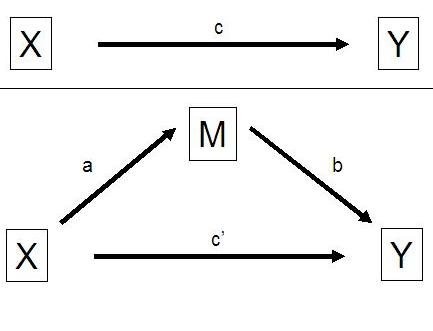
\includegraphics[scale = .5]{images/mediation_image.jpg}
    \caption{Mediation Analysis: direct and indirect effects}
    \label{fig:mediationAnalysis}
  \end{center}
\end{figure}

Mediation analysis works by testing the extent to which the variance in the outcome attributable to a predictor variable (the direct effect, or path ``c'': $Y_i \sim d_Y + cX_i + e_i$) can be explained \textit{indirectly} by the variance of two other relationships: that of the predictor variable and a third mediator (X $\rightarrow$ M, or path ``a")  and M and the outcome variable (path ``b''), controlling for the direct relationship between X and Y (path ``'c'') (see Figure ~\ref{fig:mediationAnalysis}). The mediation model can thus be denoted by two equations:

\begin{equation}
  M_i \sim d_M + aX_i + e_Mi
\end{equation}

\begin{equation}
  Y_i \sim d_Y + bM_i + c'X_i +  + e_{Yi}
\end{equation}
\bigskip

When combined, these two equations enable the calculation of the ``indirect effect'' of the predictor on the outcome, by controlling for the relationship between the mediator's effect on the outcome variable as a function of its relationship to the predictor variable.  While the direct effect measures the extent to which the dependent variable changes when the independent variable increases by one unit and the mediator variable remains unaltered, the indirect effect measures the extent to which the dependent variable changes when the independent variable is held fixed and the mediator variable changes by the amount it would have changed had the independent variable increased by one unit \citep{Bauer2006}.

The multilevel structure of the data in this study, i.e. the clustering of residuals according to team affiliation, violates the independence assumption of mediation analysis. As such, traditional multiple linear regression and path analysis will produce biased tests of the effects in the mediation model \citep{Raudenbush2002}.
%(Hox, 2002; Kreft & de Leeuw, 1998; Raudenbush & Bryk, 2002).
A multilevel mediation analysis must therefore additionally take into account variance attributable to the random effects of the model (team, in this case), and in so doing capture heterogeneity of variance in the indirect effect due to the level 2 variable \citep{Tofighi2014}.  To do this, each coefficient in the model must be random (denoted by subscript ``j''), so that the value of the coefficient varies across Level 2 units (team): \\

\begin{equation}
  M_{ij} \sim d_{Mj} + a_jX_{ij} + e_{Mij}
\end{equation}

\begin{equation}
  Y_{ij} \sim d_{Yj} + b_jM_{ij} + 'c_jX_{ij} +  + e_{Yij}
\end{equation}
\bigskip

Linear mixed effects regression models are fitted according to these equations, and estimates of mediation effects can be computed from these model parameters.  Subsequent mediation analyses were conducted using the ``mediation'' function of the Causal Mediation Analysis Package (version 4.4.5) in R.





\subsection{Post-Tournament Results}
For the following analyses, multilevel linear models were fit with Maximum Likelihood parameter estimation method using the lme4 package (Bates and Sarkar, 2006) in the R environment (R Development Core Team, 2006).  Team was included as a random effect, which allowed the intercepts and slopes of the response to vary according to team (i.e., random intercept model, see \citep{Pinheiro2000}; for an application, see \citep{Oberauer2006}). This helped statistically account for the intra-class correlation of observations within teams. Control and moderator variables were introduced into the model as fixed effects in a stepwise fashion, and model fit was judged by comparing the Akaike Information Criteria (AIC) and Bayesian Information Criteria (BIC) using a chi-squared test based on -2Log Likelihood score when possible.\footnote{The chi-squared test based on -2Log Likelihood scores was not possible when comparing models with different sample sizes.
This created difficulty when introducing covariates into the model, and subsequently reducing the number of observations} In addition, marginal and conditional $R^2$ values of equivalent models were compared and used as an indication of model effect size.\footnote{Nakagawa and Schielzeth (2013) have proposed a formula for calculating the proportion of variance explained by the fixed factor of the model (marginal $R^2$, compared to an intercept-only or null model), and the proportion of variance explained by the combination of the fixed factor plus the random factor, (conditional $R^2$, compared to the null)}





\subsubsection{1.a: Joint Action Success predicts Team Click}

In order to test the prediction that perceptions of joint-action success are positively related to team click in the post-Tournament data, the following model was constructed:

\begin{equation}
  \begin{align*}
    Team Click =  & Joint Action Success\\
              & + Individual Performance Success \\
              & + Objective Competence + Subjective Competence\\
              & + TournamentPerformanceMeasures \\
  \end{align*}
\end{equation}
\bigskip


Did perceptions of success in joint-action predict feelings of team click?  The model revealed a significant positive effect of Joint Action Success on Team Click, $\beta = .69$ ($95\% CI =  0.46, 0.89$), $SE = 0.11$, $t(13.23) = 6.20$, $p < .01$, $marginal R^2 = .53$, $conditional R^2 = .60$\footnote{Team was specified as a random effect, which allowed the slope and intercept of team click responses to vary by team. The predictor variable (Joint Action Success), moderator variables (Objective Competence and Subjective Competence), and controls (Individual Performance Success and Tournament performance measures) were introduced incrementally as fixed effects. To avoid issues of multicolinearity, Total Win Loss was excluded from the model, given the high pairwise correlation with Final Rank (.90). Pairwise correlation between all other predictor variables in the model was below .80}  Perceptions of success in individual performance components ($\beta = -.03$, $SE = .09$, $t(97) = -.33$, $p = .74$), objective ($\beta = .05$, $SE = .08$, $t(84.41) = .61$, $p = .54$) and subjective competence ($\beta = .11$, $SE = .07$, $t(87.76) = 1.57$, $p = .12$), and Tournament performance measures (Final Rank: $\beta = .02$, $SE = .04$, $t(92.85) = .58$, $p = .57$; Total Minutes: $\beta = .01$, $SE = .003$, $t(88.68) = 1.84$, $p = .07$), and Total Points: $\beta = .004$, $SE = .005$, $t(88.39) = .89$, $p = .38$)) did not significantly predict team click.  The inclusion of these fixed effects in the model did, however, significantly improve the overall model fit, as indicated by a comparison of AIC/BIC values between interactions of the model (see Table ~\ref{tab:MLM1aJointActionSuccessClick}).  Model residuals were normally distributed around zero ($W = 0.97, p = .03$), and individual cases had low influence on the model (Cook's Distances all < .25, see Appendix Figure ~\ref{fig:MLM1aAssumptions}). Results of this model support the prediction that athletes' perceptions of joint-action success correlate positively with feelings of ``team click.''


\begin{table}
\begin{center}
\begin{tabular}{l c c c }
\toprule
 & Intercept & Main effect & Controls \\
\midrule
(constant)                                                & $-0.04$  & $0.02$                & $-0.55$               \\
                                                          & $(0.15)$ & $(0.07)$              & $(0.37)$              \\
Team Performance Components                               &          & $\mathbf{0.65}^{***}$ & $\mathbf{0.66}^{***}$ \\
                                                          &          & $(0.10)$              & $(0.11)$              \\
Ind Performance Components                                &          &                       & $-0.04$               \\
                                                          &          &                       & $(0.09)$              \\
Objective Competence                                      &          &                       & $0.05$                \\
                                                          &          &                       & $(0.08)$              \\
Subjective Competence                                     &          &                       & $0.11$                \\
                                                          &          &                       & $(0.07)$              \\
Final Rank                                                &          &                       & $0.03$                \\
                                                          &          &                       & $(0.04)$              \\
Minutes Total                                             &          &                       & $0.00$                \\
                                                          &          &                       & $(0.00)$              \\
Points Total                                              &          &                       & $0.00$                \\
                                                          &          &                       & $(0.01)$              \\
Fatigue                                                   &          &                       & $0.10$                \\
                                                          &          &                       & $(0.08)$              \\
Extraverted                                               &          &                       & $0.03$                \\
                                                          &          &                       & $(0.05)$              \\
\midrule
AIC                                                       & 299.06   & 237.51                & 211.70                \\
BIC                                                       & 307.37   & 254.14                & 247.75                \\
Log Likelihood                                            & -146.53  & -112.76               & -91.85                \\
Num. obs.                                                 & 118      & 118                   & 97                    \\
\bottomrule
\multicolumn{4}{l}{\scriptsize{Coefficients with $p < 0.05$ in \textbf{bold}. Marginal $R^2 = .56$, Conditional $R^2 = .61$}}
\end{tabular}
\caption{Prediction 1: Team Performance Components predicts Team Click in the Post-Tournament survey data.}
\label{tab:MLM1aJointActionSuccessClick}
\end{center}
\end{table}





\subsubsection{1.b Team Performance Expectations predict Team Click}

To assess the prediction that more positive violation of expectations around team performance correlates with higher levels of team click, the following model was constructed:

\begin{equation}
  \begin{align*}
    Team Click =  & Team Performance Expectations \\
              &+ Individual Performance Expectations \\
              &+ Objective Competence + Subjective Competence \\
              &+ Tournament performance measures \\
  \end{align*}
\end{equation}

Expectations around individual performance, objective and subjective competence, and Tournament performance measures were introduced to the model as controls (fixed effects), while team was introduced as a random (level 2) effect.

Results of the model revealed a significant positive relationship between Team Performance Expectations and Team Click, $\beta = .52$ ($95\% CI =  0.28, 0.73$), $SE = 0.12$, $t(4.23) = 4.23$, $p < .001$, $marginal R^2 = .40$, $conditional R^2 = .56$.
Expectations around individual performance ($\beta = .04$, $SE = .08$, $t(86.26) = .46$, $p = .65$), objective ($\beta = .01$, $SE = .09$, $t(84.89) = .13$, $p = .89$) and subjective competence ($\beta = .12$, $SE = .07$, $t(91) = 1.62$, $p = .11$), and Tournament performance measures (Final Rank: $\beta = .08$, $SE = .05$, $t(44.33) = 1.72$, $p = .09$;
Total Minutes: $\beta = .004$, $SE = .003$, $t(87.05) = 1.00$, $p = .32$); Total Points: $\beta = .001$, $SE = .005$, $t(84.94) = .21$, $p = .84$)) did not significantly predict team click.  The inclusion of these effects did, however, improve the model fit, as indicated by the reduced AIC and increased marginal $R^2$ value (see Appendix Table ~\ref{tab:MLM1bteamExpectationsClick} for the various iterations of the model).  Model residuals were normally distributed around zero ($W = 0.98, p = .30$), and individual cases had low influence on the model (Cook's Distances all < .25, see Appendix Figure ~\ref{fig:MLM1bAssumptions}).  These results provide support for the prediction that more positive violations of expectations around team performance predict feelings of team click.



\begin{table}
\begin{center}
\begin{tabular}{l c c c }
\toprule
 & Intercept & Main effect & Controls \\
\midrule
(constant)                                 & $-0.04$  & $-0.00$               & $\mathbf{-0.79}^{*}$  \\
                                           & $(0.15)$ & $(0.09)$              & $(0.40)$              \\
Team Performance Vs Expectations           &          & $\mathbf{0.50}^{***}$ & $\mathbf{0.51}^{***}$ \\
                                           &          & $(0.11)$              & $(0.12)$              \\
Ind Performance Vs Expectations            &          &                       & $0.02$                \\
                                           &          &                       & $(0.08)$              \\
Objective Competence                       &          &                       & $0.02$                \\
                                           &          &                       & $(0.08)$              \\
Subjective Competence                      &          &                       & $0.12$                \\
                                           &          &                       & $(0.07)$              \\
Final Rank                                 &          &                       & $\mathbf{0.09}^{*}$   \\
                                           &          &                       & $(0.05)$              \\
Minutes Total                              &          &                       & $-0.00$               \\
                                           &          &                       & $(0.00)$              \\
Points Total                               &          &                       & $0.00$                \\
                                           &          &                       & $(0.01)$              \\
Fatigue                                    &          &                       & $\mathbf{0.18}^{*}$   \\
                                           &          &                       & $(0.09)$              \\
Extraverted                                &          &                       & $0.06$                \\
                                           &          &                       & $(0.05)$              \\
\midrule
AIC                                        & 299.06   & 268.43                & 228.63                \\
BIC                                        & 307.37   & 285.06                & 264.68                \\
Log Likelihood                             & -146.53  & -128.22               & -100.32               \\
Num. obs.                                  & 118      & 118                   & 97                    \\
Num. groups: team                          & 15       & 15                    & 14                    \\
\bottomrule
\multicolumn{4}{l}{\scriptsize{Coefficients with $p < 0.05$ in \textbf{bold}. Marginal $R^2 = .40$, Conditional $R^2 = .56$}}
\end{tabular}
\caption{Prediction 5: Team Performance Vs Expectations predicts Team Click in the Post-Tournament survey data (n = 97).}
\label{tab:MLM1bteamExpectationsClick}
\end{center}
\end{table}


\subsubsection{1.c Team Performance Expectations moderates the effect of Joint Action Success on team Click}

If both perceptions of joint-action success and positive violations of expectations predict team click, do these two predictors interact to predict click? Is team click higher for individuals whose perceived success in joint action was also a more positive violation of performance expectation? To test this possibility, the interaction term (Joint Action Success \times Team Performance Expectations) was included in model 1a as follows::

\begin{equation}
  \begin{align*}
    Team Click =  & Joint Action Success \times Team Performance Expectations \\
              &+ Individual Performance Success \\
              &+ Individual Performance Expectations \\
              &+ Objective Competence + Subjective Competence  \\
              &+ Tournament performance measures \\
  \end{align*}
\end{equation}
\bigskip
The inclusion of the interaction term failed to improve upon the fit of the previous model, judging by the relative goodness of fit, $AIC(1.c) = 217.91$ compared to $AIC(1.a) = 209.48$, $SD = .52 $, $\chi^2(18, N = 97) = 3.56$, $ p =.74$.  Results revealed that the interaction between Joint Action Success and Team Performance Expectations was not significant, $\beta = .002$ ($95\% CI =  -0.0062, 0.0063$), $SE = 0.08$, $t(39.7) = .026$, $p = .98$, $marginal R^2 = .56$, $conditional R^2 = .65$ (see Appendix, Table ~\ref{tab:MLM1cPerformanceClickInteraction}).


%\textit{See appendix A for details about model assumptions}.
%\newpage
%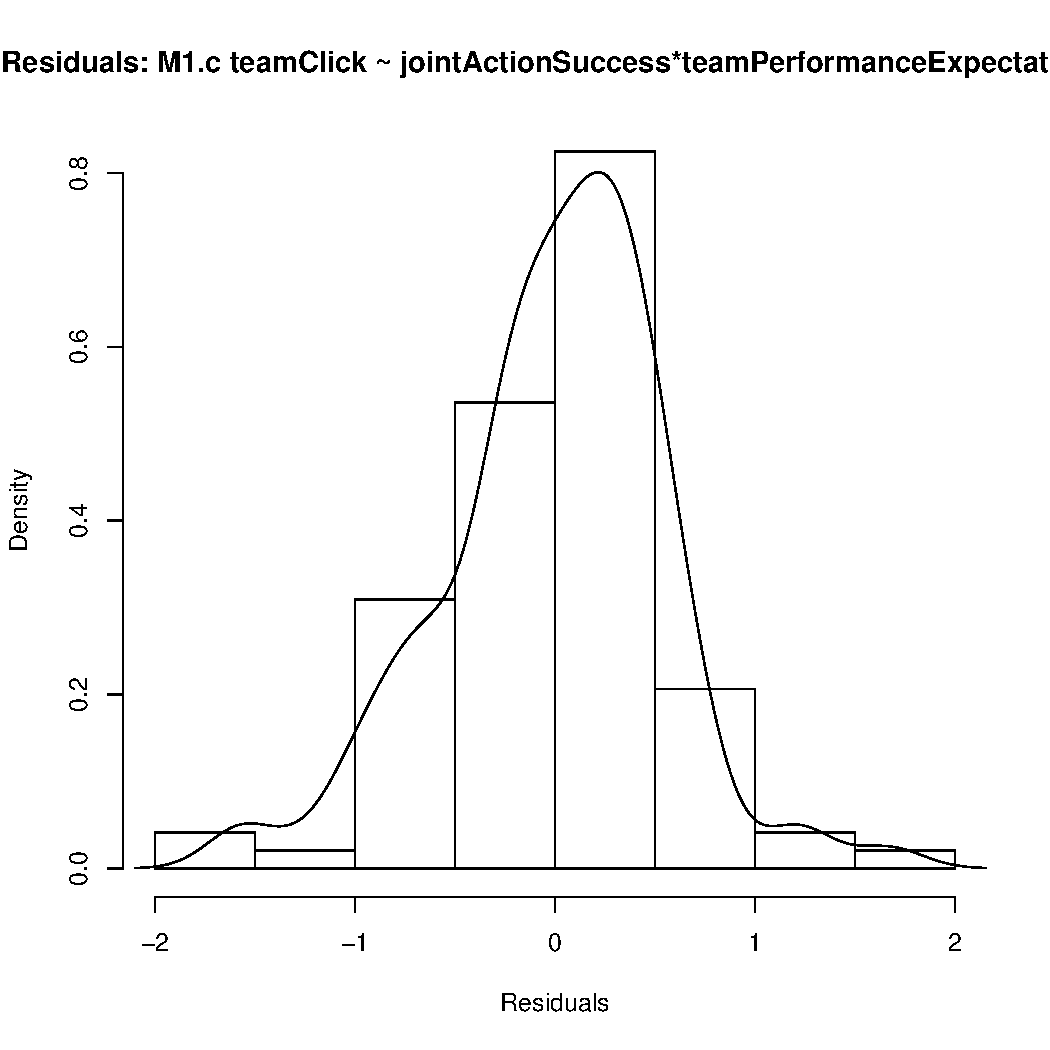
\includegraphics[scale =.4]{../images/MLM1cHist.pdf}
%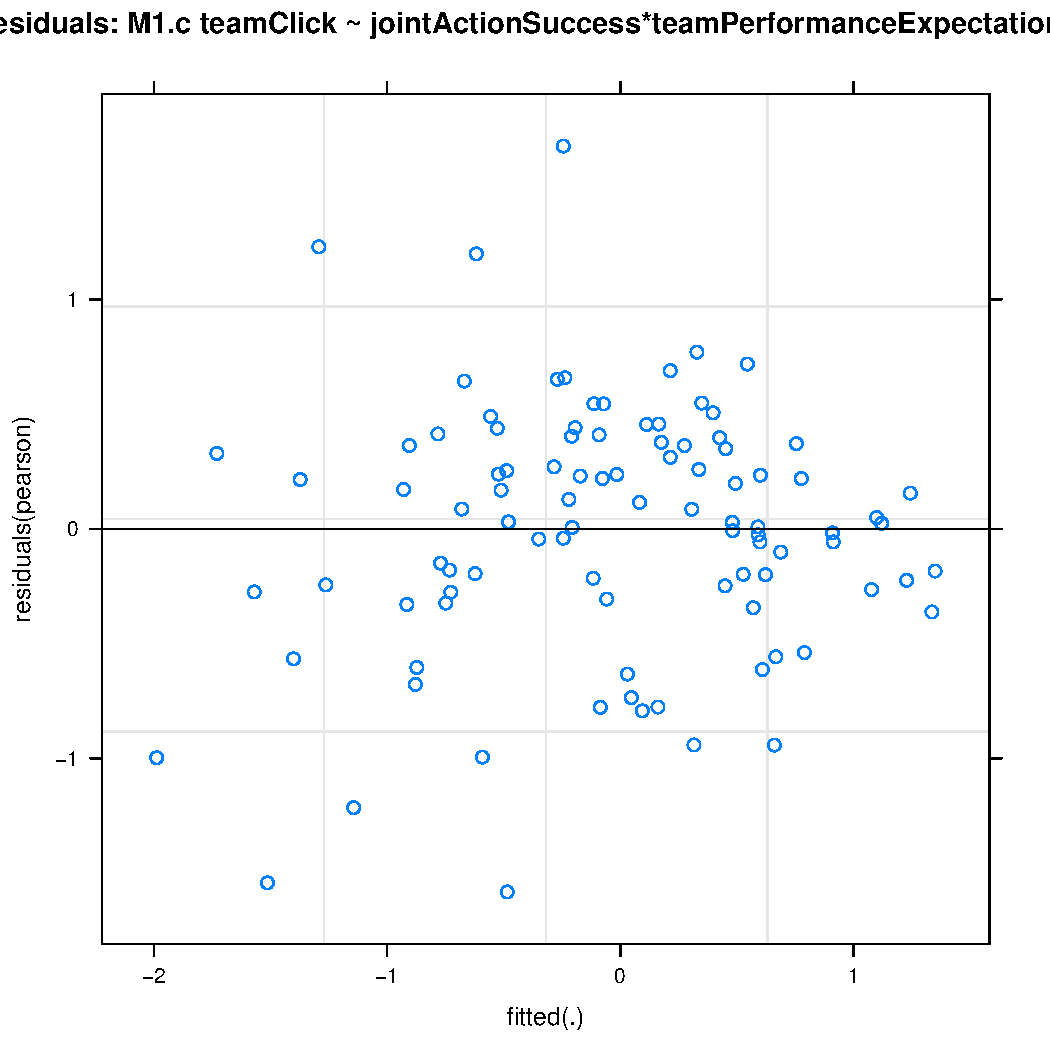
\includegraphics[scale =.4]{../images/MLM1cScatter.pdf}
%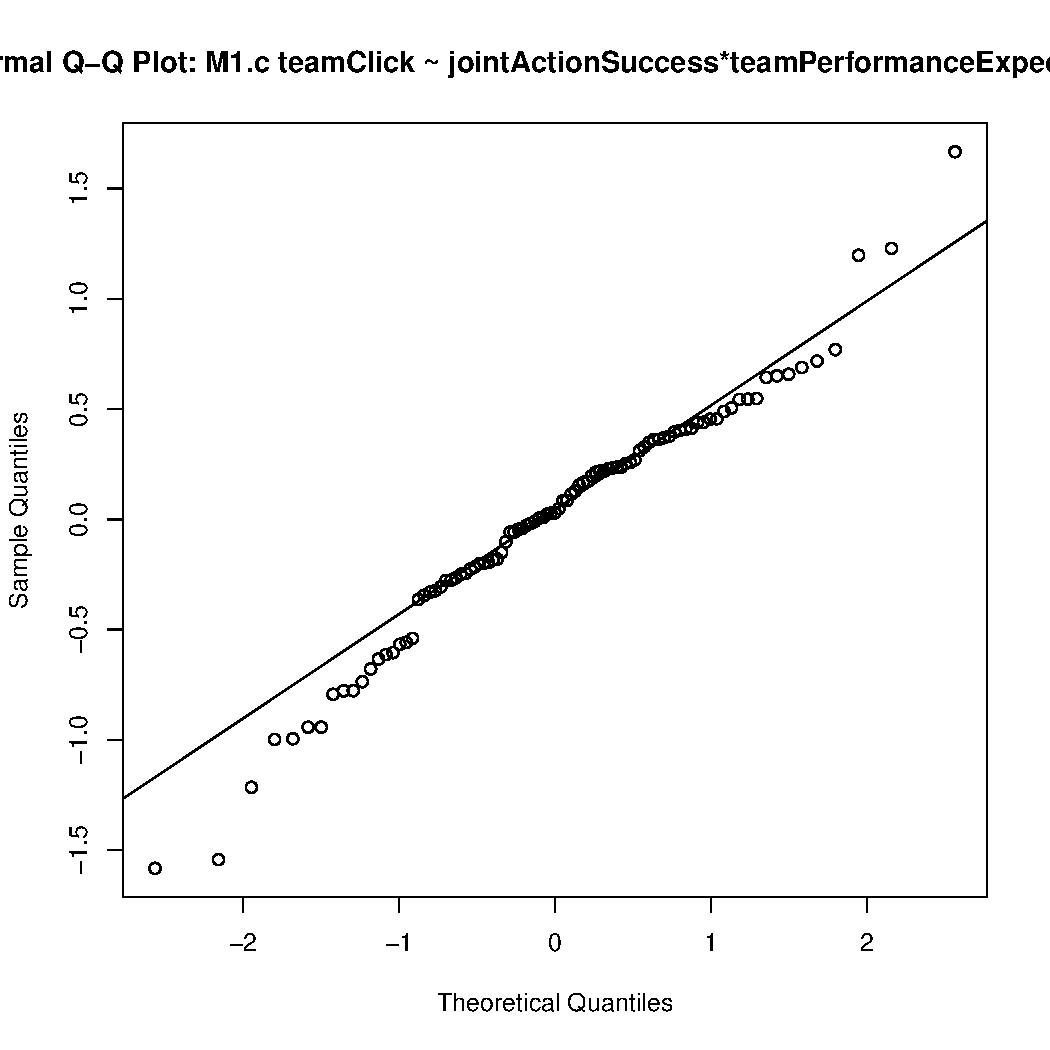
\includegraphics[scale =.4]{../images/MLM1cQQNorm.pdf}
%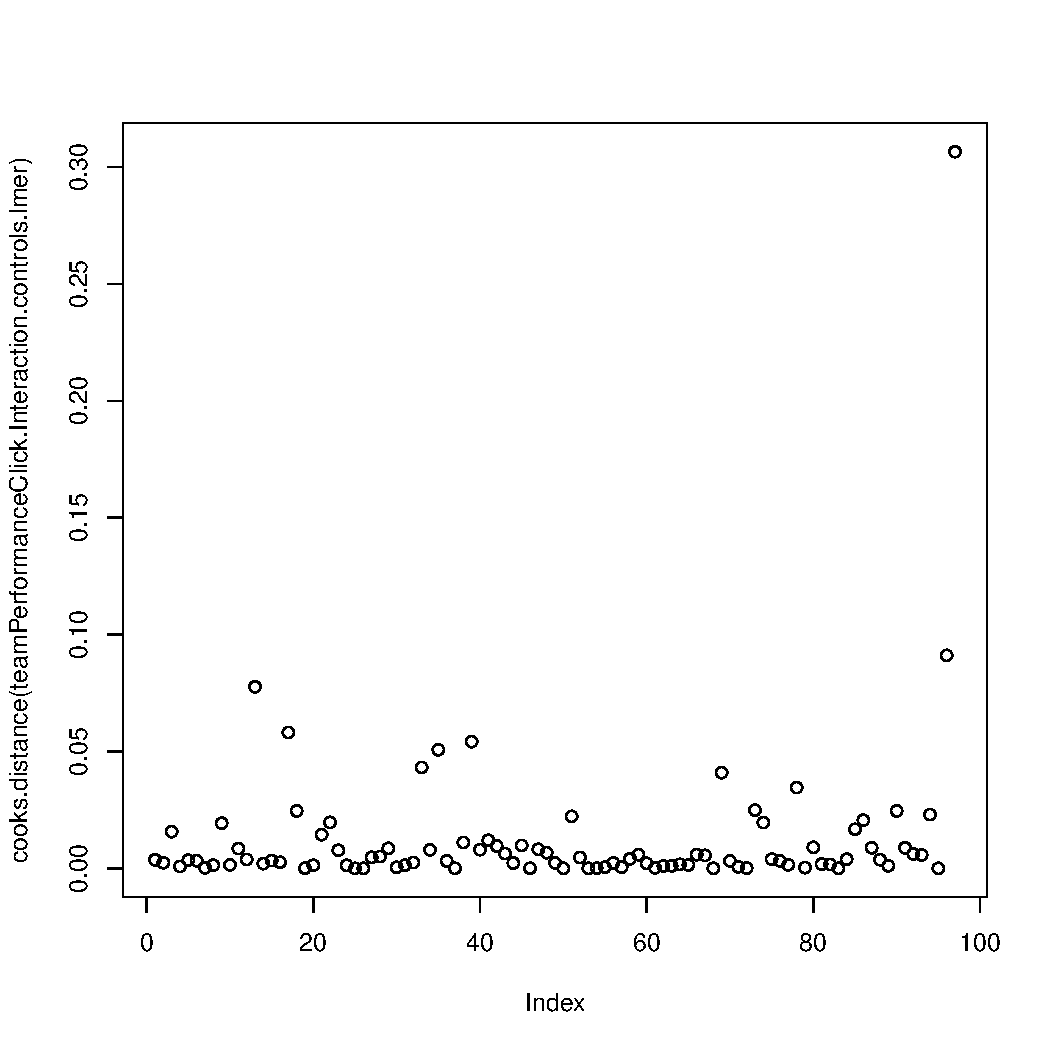
\includegraphics[scale =.4]{../images/MLM1cCooksD.pdf}

%\textit{problem here: increase in marginal and conditional R^2 values, perhaps due to adding additional variables into the model}
%The interaction did not improve the model fit,
%Nor did adding teamPerformance7 on its own into the model...
%But an interaction alone was significant

Findings from the first collection of models generally supported predictions. Team performance factors\nobreakdashperceptions of team component performance success and team performance relative to prior expectations\nobreakdashbut not individual performance factors significantly predicted team click, when controlling for subjective and objective competence, and Tournament performance measures.  The interaction effect of joint-action success and team performance expectations violation on team click was not significant.  Additionally, the low coefficient value for the model in which teamPerformanceExpectations predicted team click was low, indicating that this result should be treated with some caution.  Taken together, however, these results provide evidence for the predictions that perceptions of joint-action success is linked to feelings of team click.  Team performance expectations do not interact with perceptions of joint action to enhance feelings of team click, but rather function independently to predict team click, with those athletes who were experienced more positive violations of expectations also reporting higher levels of team click.






\subsubsection{2.a Team Click predicts Social Bonding}
The relationship between team click and social bonding was tested in the post-Tournament data. A linear mixed effects regression model was constructed with team as random effect, Team Click as fixed effect (predictor), and Social Bonding as outcome variable:

\begin{equation}
  \begin{align*}
    Social Bonding   =& Team Click\\
                    &+ Objective Competence + Subjective Competence  \\
                    &+ Tournament performance measures \\
  \end{align*}
\end{equation}
\bigskip

Controlling for Tournament performance measures and objective and subjective competence, the model revealed a significant relationship between team click and social bonding, $\beta = .67$ ($95\% CI =  .51, .84$), $SE = 0.08$, $t(16.01) = 8.22$, $p < .0001$, $marginal R^2 = .49$, $conditional R^2 = .51$ (see Table ~\ref{tab:MLM2aTeamClickBonding}).  Model residuals were normally distributed around zero ($W = 0.98, p = .15$), and individual cases had low influence on the model (Cook's Distances all < .15, see Appendix Figure ~\ref{fig:MKM2aAssumptions}).  This model supported the prediction that, following intense exertive joint-activity, higher levels of team click are associated with higher levels of social bonding.



% Table created by stargazer v.5.2 by Marek Hlavac, Harvard University. E-mail: hlavac at fas.harvard.edu
% Date and time: Mon, Jun 26, 2017 - 20:48:41
\begin{table}[!htbp] \centering 
  \caption{socialBonding = teamClick} 
  \label{tab:MLM2aTeamClickBonding} 
\begin{tabular}{@{\extracolsep{5pt}}lccc} 
\\[-1.8ex]\hline 
\hline \\[-1.8ex] 
 & \multicolumn{3}{c}{\textit{Dependent variable:}} \\ 
\cline{2-4} 
\\[-1.8ex] & \multicolumn{3}{c}{socialBonding} \\ 
\\[-1.8ex] & (1) & (2) & (3)\\ 
\hline \\[-1.8ex] 
 (constant) & $-$0.01 & $-$0.0002 & 0.21 \\ 
  & (0.10) & (0.07) & (0.27) \\ 
  & & & \\ 
 teamClick &  & 0.64$^{***}$ & 0.67$^{***}$ \\ 
  &  & (0.08) & (0.08) \\ 
  & & & \\ 
 objectiveCompetence &  &  & 0.04 \\ 
  &  &  & (0.08) \\ 
  & & & \\ 
 subjectiveCompetence &  &  & 0.12 \\ 
  &  &  & (0.07) \\ 
  & & & \\ 
 finalRank &  &  & $-$0.01 \\ 
  &  &  & (0.04) \\ 
  & & & \\ 
 minutesTotal &  &  & $-$0.003 \\ 
  &  &  & (0.004) \\ 
  & & & \\ 
 pointsTotal &  &  & $-$0.002 \\ 
  &  &  & (0.01) \\ 
  & & & \\ 
\hline \\[-1.8ex] 
Marginal R-squared &  &  & .49 \\ 
Conditional R-squared &  &  & .51 \\ 
Observations & 118 & 118 & 97 \\ 
Log Likelihood & $-$151.95 & $-$118.76 & $-$97.75 \\ 
Akaike Inf. Crit. & 309.90 & 249.53 & 217.50 \\ 
Bayesian Inf. Crit. & 318.21 & 266.15 & 245.82 \\ 
\hline 
\hline \\[-1.8ex] 
\textit{Note:}  & \multicolumn{3}{r}{$^{*}$p$<$0.05; $^{**}$p$<$0.01; $^{***}$p$<$0.001} \\ 
\end{tabular} 
\end{table} 





\subsubsection{3.a Joint Action Success predicts Social Bonding}

In light of evidence for significant relationships between joint-action success and team click, and team click and social bonding, the direct relationship between joint-action success and social bonding was assessed. Controlling for perceptions of success in individual performance, objective and subjective competence, and Tournament performance measures, the model revealed a significant effect of joint-action success on social bonding, $\beta = .45$ ($95\% CI =  .17, .73$), $SE = .14$, $t(23.4) = 3.19$, $p < .01$, $marginal R^2 = .27$, $conditional R^2 = .42$.  The model also revealed a significant positive effect of subjective measures of competence on social bonding, $\beta = .18$ ($95\% CI =  .03, .35$), $SE = .08$, $t(90.86) = 2.26$, $p = .03$ (full results in Table ~\ref{tab:MLM3aJointActionSuccessBonding}).

While Levene's Test for Equality of Variance indicated that the assumption of homoscedasticity was met at the group-level, $F(13,83) = .80, p = .66$, overall model residuals were non-normally distributed ($W = 0.95, p = .0007$), owing to relatively large negative skew (-.87) (see Appendix Figure ~\ref{fig:MLM3aAssumptions}). Non-normally distributed residuals are problematic as they may influence the model's ability to generate accurate parameter estimates . Two data manipulation techniques were considered in order to normalise residuals and therefore preserve the estimates of the model: exclusion of outliers and transformation of the outcome variable.  Transformation of the outcome variables was the preferred method over outlier exclusion, due to the cost involved in removing observations that may be of potential theoretical relevance to the scientific investigation \citep{Rousseeuw2011}. Nonetheless, for this first phase of analysis, both outlier exclusion and transformation manipulations of the data were performed and reported.

Exclusion of outliers according to Tukey's method (observations above and below 1.5x the Inter Quartile Range (IQR), see \citep{Tukey1977}) appeared to improve the model fit, $\beta = .26$ ($95\% CI =  .05, .47$), $SE = 0.004$, $t(9.78) = 3.66$, $p < .01$, $marginal R^2 = .18$, $conditional R^2 = .34$.
The distribution of model residuals appeared to improve, but still violated the assumption of normality ($Shapiro-Wilk = 0.96, p = .009$).  Individual cases had low influence on the model (Cook's Distances all < .10).

Due to the \textit{positive} skew of the model residuals, the outcome variable was transformed by taking the log of the reversed scores of the outcome variable, i.e. $log10(k - y)$, where $k$ is a constant value from which each score for $y$ is subtracted so that the distribution of the outcome variable is reversed\citep{Howell2012}.\footnote{Reversing the distribution of the outcome variable allows the logarithmic function to normalise the distribution of the variable, by pushing them from the left hand side of the distribution towards the centre}  Transformed values were then returned to their original direction for analysis\citep{Field2012}.  Rebuilding the model with a log-transformed outcome variable appeared to improve the fit of the model more than the outlier-removed model, and avoided the removal of any observations.
The distribution of residuals appeared more normal, ($W = 0.97, p = .04$), and the R-squared values for the model improved, $marginal R^2 = .27$, $conditional R^2 = .43$ (see Table ~\ref{tab:MLM3aJointActionSuccessBonding} for results of all three models, and Appendix Figures ~\ref{fig:MLM3aAssumptions}\nobreakdash~\ref{fig:MLM3aLogAssumptions}).  Results of the log-transformed model indicated that the non-normally distributed residuals of the original model did not impact the estimates of the model. As such, the results of these models were taken as evidence for a significant positive relationship between perceptions of joint-action success and feelings of social bonding.


% Table created by stargazer v.5.2 by Marek Hlavac, Harvard University. E-mail: hlavac at fas.harvard.edu
% Date and time: Mon, Jun 26, 2017 - 21:18:41
\begin{table}[!htbp] \centering 
  \caption{socialBonding = jointActionSuccess} 
  \label{tab:MLM3aJointActionSuccessBonding} 
\footnotesize 
\begin{tabular}{@{\extracolsep{5pt}}lccc} 
\\[-1.8ex]\hline 
\hline \\[-1.8ex] 
 & \multicolumn{3}{c}{\textit{Dependent variable:}} \\ 
\cline{2-4} 
\\[-1.8ex] & socialBonding & bondingPostFactorOut & bondingPostFactorLogReturned \\ 
 &  & outliers removed & log-transformed \\ 
\\[-1.8ex] & (1) & (2) & (3)\\ 
\hline \\[-1.8ex] 
 (constant) & $-$0.06 & $-$0.06 & 1.97$^{***}$ \\ 
  & (0.31) & (0.31) & (0.13) \\ 
  & & & \\ 
 jointActionSuccess & 0.45$^{**}$ & 0.45$^{**}$ & 0.20$^{***}$ \\ 
  & (0.14) & (0.14) & (0.06) \\ 
  & & & \\ 
 indPerformanceSuccess & 0.05 & 0.05 & $-$0.001 \\ 
  & (0.11) & (0.11) & (0.05) \\ 
  & & & \\ 
 objectiveCompetence & 0.07 & 0.07 & 0.04 \\ 
  & (0.10) & (0.10) & (0.04) \\ 
  & & & \\ 
 subjectiveCompetence & 0.19$^{*}$ & 0.19$^{*}$ & 0.09$^{*}$ \\ 
  & (0.08) & (0.08) & (0.03) \\ 
  & & & \\ 
 finalRank & $-$0.02 & $-$0.02 & $-$0.01 \\ 
  & (0.05) & (0.05) & (0.02) \\ 
  & & & \\ 
 minutesTotal & 0.002 & 0.002 & 0.001 \\ 
  & (0.004) & (0.004) & (0.002) \\ 
  & & & \\ 
 pointsTotal & $-$0.001 & $-$0.001 & $-$0.002 \\ 
  & (0.01) & (0.01) & (0.003) \\ 
  & & & \\ 
\hline \\[-1.8ex] 
Marginal R-squared & .27 & .18 & .28 \\ 
Conditional R-squared & .42 & .34 & .43 \\ 
Observations & 97 & 97 & 97 \\ 
Log Likelihood & $-$113.05 & $-$113.05 & $-$29.49 \\ 
Akaike Inf. Crit. & 250.10 & 250.10 & 82.98 \\ 
Bayesian Inf. Crit. & 281.00 & 281.00 & 113.87 \\ 
\hline 
\hline \\[-1.8ex] 
\textit{Note:}  & \multicolumn{3}{r}{$^{*}$p$<$0.05; $^{**}$p$<$0.01; $^{***}$p$<$0.001} \\ 
\end{tabular} 
\end{table} 



\subsubsection{3.b Team Performance Expectations predicts Social Bonding} % very small effect

The direct relationship between expectations around team performance and social bonding was also tested.  The model revealed a significant positive relationship between Team Performance Expectations and Social Bonding, $\beta = .34$ ($95\% CI =  .06, .63$), $SE = .14$, $t(13.79) = 2.38$, $p = .03$, $marginal R^2 = .20$, $conditional R^2 = .40$.  The model also revealed a significant positive effect of Subjective Competence on Social Bonding, $\beta = .19$ ($95\% CI =  .02, .36$), $SE = .08$, $t(90.37) = 2.24$, $p = .03$, such that athletes who provided higher ratings of their own technical competence in rugby (measured before the Tournament) reported higher levels of social bonding.

Model residuals were not normally distributed, ($W = 0.91, p < .0001$), owing to large negative skew ($-1.33$) and high kurtosis ($.49$). Re-running the model with a log-transformed outcome variable appeared to make the best improvement to model residuals more than the outlier-removed model (see Table ~\ref{tab:MLM3bExpectationsBonding}). In the log-transformed model, the distribution of model residuals appeared most normal,  ($W = 0.97, p = .02$), and the R-squared values for the model improved, $marginal R^2 = .23$, $conditional R^2 = .44$.  Individual cases had low influence on the model (Cook's Distances all < .15, see Appendix Figures ~\ref{fig:MLM3bAssumptions} and ~\ref{fig:MLM3bLogAssumptions} for a comparison of model assumptions between the original and log-transformed model). Owing to non-normally distributed residuals, this model does not provide robust support for the prediction that team performance expectation violations relates directly to social bonding.

Results outlined above demonstrate significant relationships between Joint-Action Success and Team Click, Team Click and Social Bonding, and a direct relationship between Joint-Action Success and Social Bonding. Results of models linking Team Performance Expectations, Team Click, and Social Bonding were lest robust, and should be treated with caution.


%Outlier exclusion
%Exclusion of outliers improved the distribution of residuals, ($W = 0.96, p = .007$), and individual cases had low influence on the model (Cook's Distances all < .15).  The significant positive effect of teamPerformanceExpectations on socialBonding remained in the adjusted model, $\beta = .01$ ($95\% CI =  .003, .02$), $SE = .004$, $t() = 2.65$, $p = .03$, $marginal R^2 = .19$, $conditional R^2 = .40$.  The effect of Subjective Competence on socialBonding was no longer significant, $\beta = .12$ ($95\% CI =  -.0004, .24$), $SE = .06$, $t(90.44) = 1.95$, $p = .06$.

\newgeometry{margin=0.5cm}

% Table created by stargazer v.5.2 by Marek Hlavac, Harvard University. E-mail: hlavac at fas.harvard.edu
% Date and time: Tue, Jun 27, 2017 - 17:01:54
\begin{table}[!htbp] \centering 
  \caption{M3.b socialBonding = teamPerformanceExpectations} 
  \label{tab:MLM3bExpectationsBonding} 
\scriptsize 
\begin{tabular}{@{\extracolsep{5pt}}lccc} 
\\[-1.8ex]\hline 
\hline \\[-1.8ex] 
 & \multicolumn{3}{c}{\textit{Dependent variable:}} \\ 
\cline{2-4} 
\\[-1.8ex] & socialBonding & bondingPostFactorOut & bondingPostFactorLogReturned \\ 
 &  & outliers removed & log-transformed \\ 
\\[-1.8ex] & (1) & (2) & (3)\\ 
\hline \\[-1.8ex] 
 (constant) & $-$1.67$^{*}$ & $-$1.18$^{*}$ & 1.19$^{***}$ \\ 
  & (0.73) & (0.53) & (0.31) \\ 
  & & & \\ 
 teamPerformanceExpectations & 0.01$^{*}$ & 0.01$^{**}$ & 0.01$^{**}$ \\ 
  & (0.01) & (0.004) & (0.003) \\ 
  & & & \\ 
 individualPerformanceExpectations & 0.004 & 0.001 & 0.001 \\ 
  & (0.004) & (0.003) & (0.002) \\ 
  & & & \\ 
 objectiveCompetence & 0.03 & 0.02 & 0.02 \\ 
  & (0.10) & (0.07) & (0.04) \\ 
  & & & \\ 
 subjectiveCompetence & 0.19$^{*}$ & 0.12 & 0.08$^{*}$ \\ 
  & (0.09) & (0.06) & (0.04) \\ 
  & & & \\ 
 finalRank & 0.08 & 0.10 & 0.04 \\ 
  & (0.13) & (0.09) & (0.05) \\ 
  & & & \\ 
 minutesTotal & 0.0003 & 0.001 & 0.0001 \\ 
  & (0.004) & (0.003) & (0.002) \\ 
  & & & \\ 
 pointsTotal & $-$0.04 & $-$0.06 & $-$0.03 \\ 
  & (0.09) & (0.06) & (0.04) \\ 
  & & & \\ 
 pointsTotal & $-$0.001 & $-$0.004 & $-$0.002 \\ 
  & (0.01) & (0.005) & (0.003) \\ 
  & & & \\ 
\hline \\[-1.8ex] 
Marginal R-squared & .20 & .19 & .23 \\ 
Conditional R-squared & .40 & .40 & .44 \\ 
Observations & 97 & 91 & 97 \\ 
Log Likelihood & $-$117.26 & $-$77.84 & $-$32.42 \\ 
Akaike Inf. Crit. & 260.52 & 181.67 & 90.85 \\ 
Bayesian Inf. Crit. & 293.99 & 214.31 & 124.32 \\ 
\hline 
\hline \\[-1.8ex] 
\textit{Note:}  & \multicolumn{3}{r}{$^{*}$p$<$0.05; $^{**}$p$<$0.01; $^{***}$p$<$0.001} \\ 
\end{tabular} 
\end{table} 

\restoregeometry



\subsubsection{4.a Mediation analysis: Joint Action Success predicts Social Bonding, mediated by Team Click}
Mediation analyses were conducted using linear mixed effects regressions in the Causal Mediation Analysis package in R (Version 4.4.5).  To make inferences concerning the average indirect and total effects, quasi-Bayesian Markov Chain Monte Carlo (MCMC) method based on normal approximation and 1000 simulations was used to estimate the 95\% Confidence Intervals \citep{Tofighi2016a,Imai2010}. MCMC estimation is a form of non-parametric bootstrapping whereby the sampling distribution for the effect of interest is not assumed to be normal but is instead simulated from the model estimates and their asymptotic variances and covariances \cite{Preacher2008}.

Results of the mediation analysis revealed significant average indirect effect of Joint Action Success on Social Bonding attributable to Team Click, $\beta = .37, 95\% CI = 0.20 , 0.59, p < .001$.  When controlling for the effect of team click on social bonding, the average direct effect between Joint Action Success and Social Bonding was no longer significant, $\beta = -.006, 95\% CI = -.27 , .23, p = .96 $ (see Figure ~\ref{fig:MLM4aMediationAnalysis}). The direct effect diminished such that including Joint Action Success in the model produced a total effect that was marginally \textit{smaller} than the indirect effect alone, $\beta = .36, 95\% CI = .13 , .61, p = .01$. These results suggest that feelings of team click fully mediate the relationship between perceptions of joint-action success and social bonding.


%Residuals of the mediation model were normally distributed around zero, ($W = 0.99, p < .28$, see Figure ~\ref{fig:MLM4aAssumptions} for model assumptions).



\subsubsection{4.b Mediation analysis: Team Performance Expectations predicts Social Bonding, mediated by Team Click}

Post-Tournament results also demonstrate a significant positive relationship between Team Performance Expectations and Team Click. The model generated for relationships between between Team Performance Expectations and Social Bonding, however, was not robust to the demands of model assumptions.   Nonetheless, mediation analysis was used to test the possibility that Team Click mediated the effects of Team Performance Expectations on Social Bonding.

Results of the mediation analysis revealed significant average indirect effect of Team Performance Expectations on Social Bonding attributable to Team Click, $\beta = .36, 95\% CI = 0.17 , 0.62, p < .0001$.  When controlling for the effect of Team Click on Social Bonding, the average direct effect between Team Performance Expectations and Social Bonding was no longer significant, $\beta = -.07, 95\% CI = -.27 , .12, p = .84 $ (see Figure ~\ref{fig:MLM4bMediationAnalysis}). The total effect of the model was significant $\beta = .29, 95\% CI = .02 , .57, p = .04$.  This model, as with model 4.a above, indicated that Team Click fully mediated the relationship between Team Performance Expectations and Social Bonding.


Again, the results of this mediation model should be treated with caution, given the fact that the mediation model is composed of a non-robust statistical model (i.e., path ```'c'').

\begin{figure}[htbp]
  \centering
  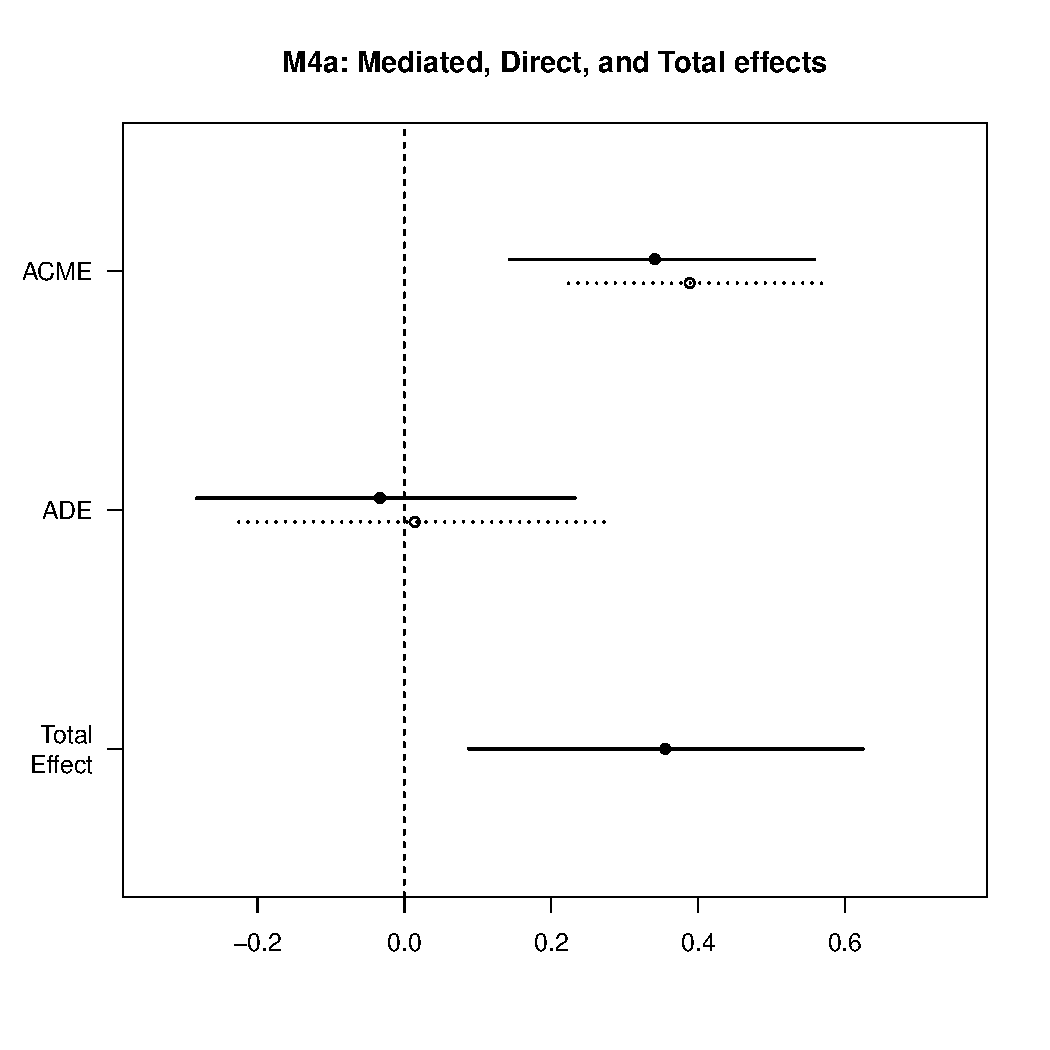
\includegraphics[scale = .5]{images/MLM4aMediationEffects.pdf}
  \caption{M4a Mediation Analysis}
  \label{fig:MLM4aMediationAnalysis}
\end{figure}

\begin{figure}[htbp]
  \centering
  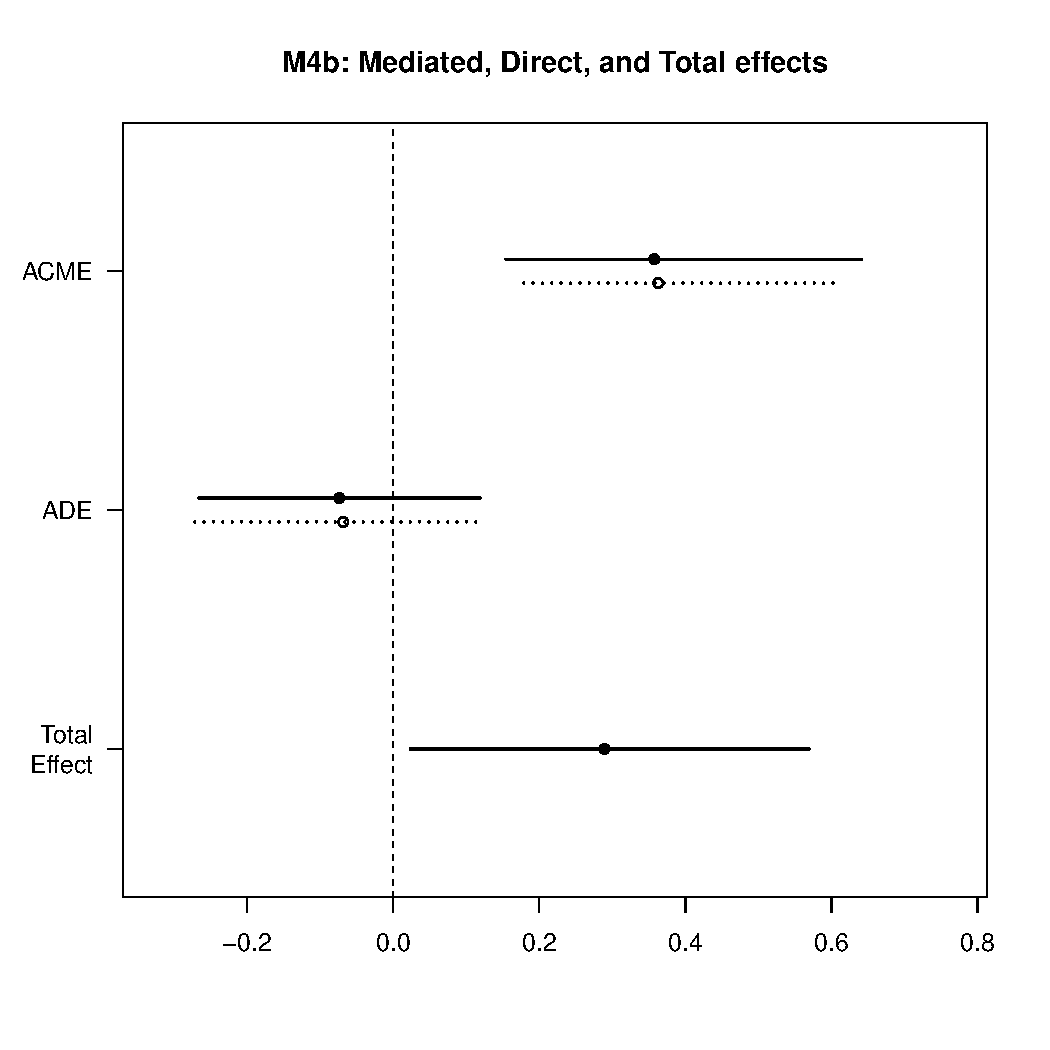
\includegraphics[scale = .5]{images/MLM4bMediationEffects.pdf}
  \caption{M4b Mediation Analysis}
  \label{fig:MLM4bMediationAnalysis}
\end{figure}





%\begin{figure}[htbp]
%  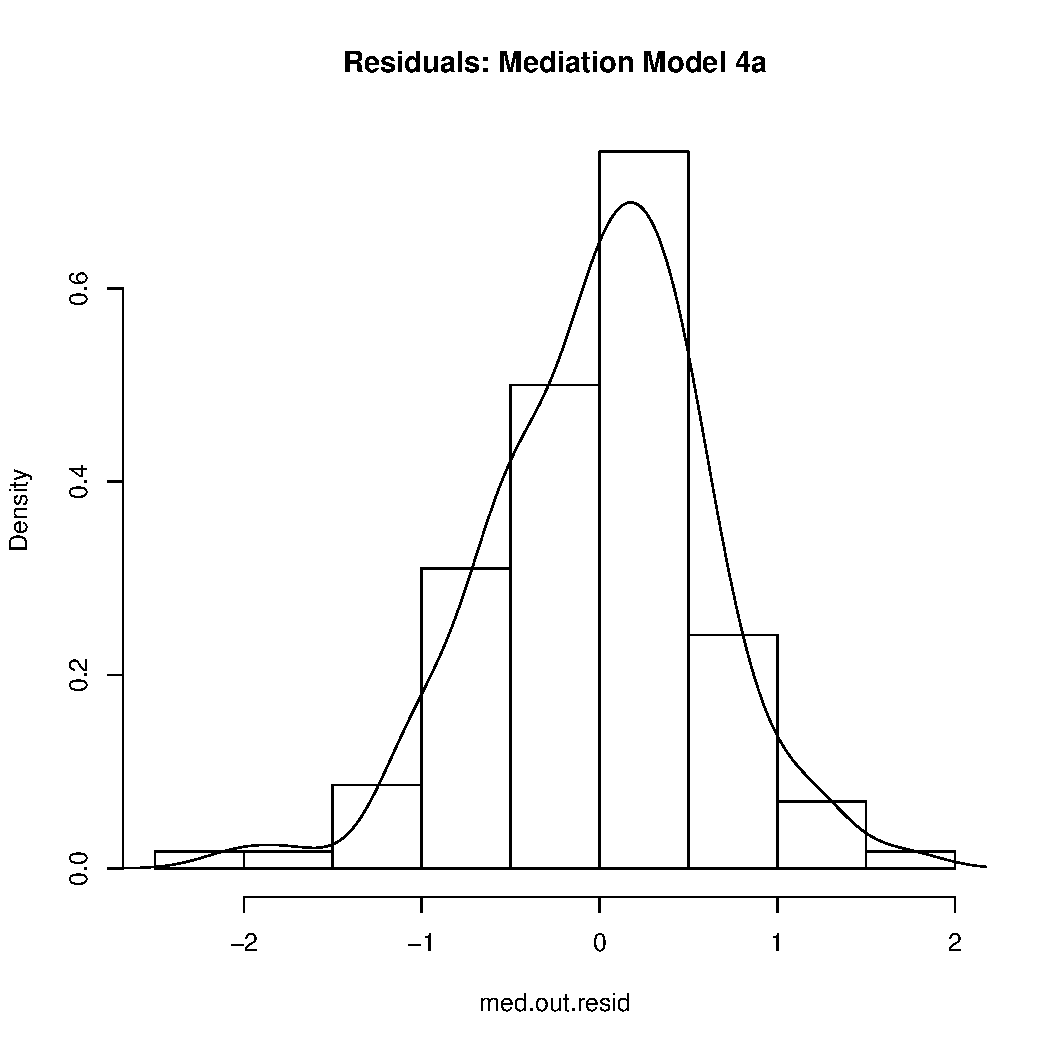
\includegraphics{finalDocuments/images/MLM4aResiduals.pdf}
%  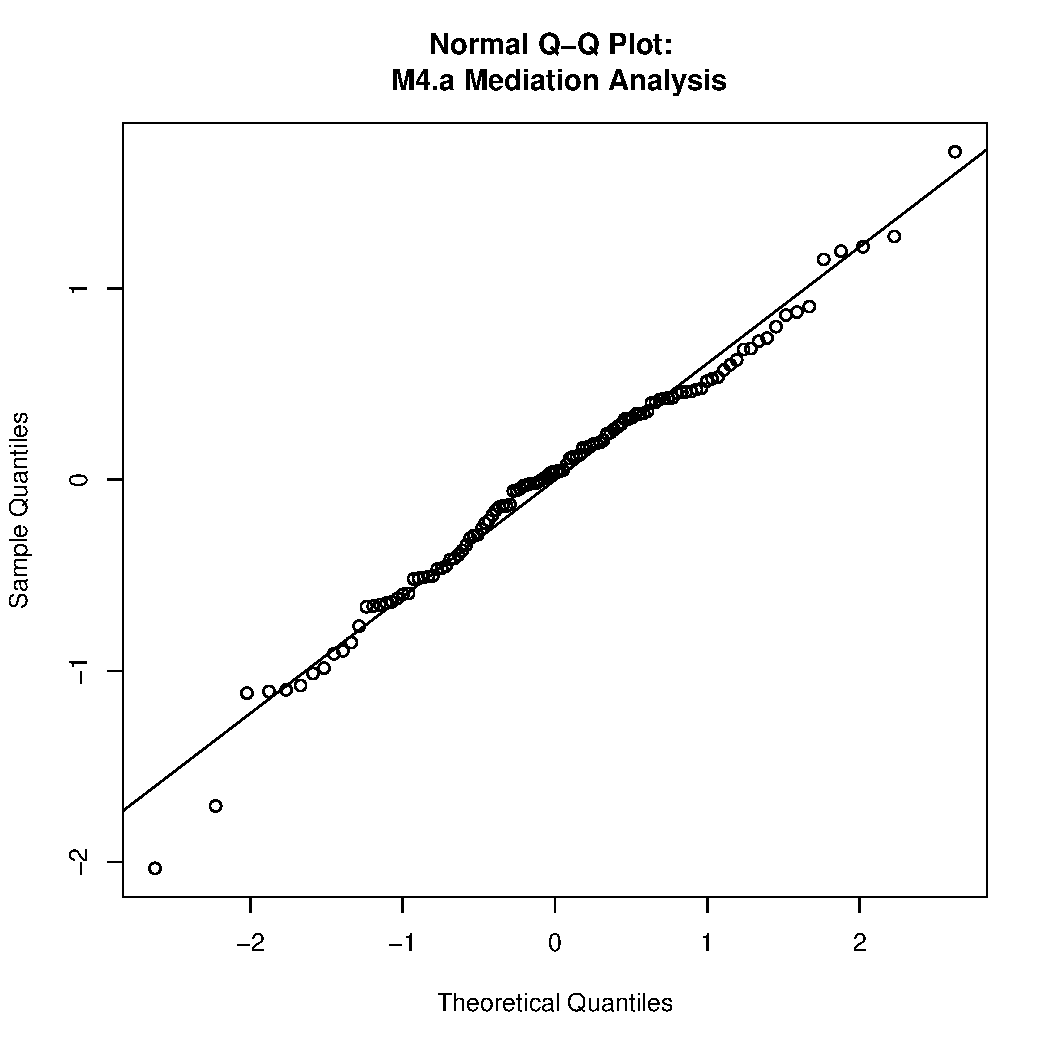
\includegraphics{finalDocuments/images/MLM4aQQNorm.pdf}
%  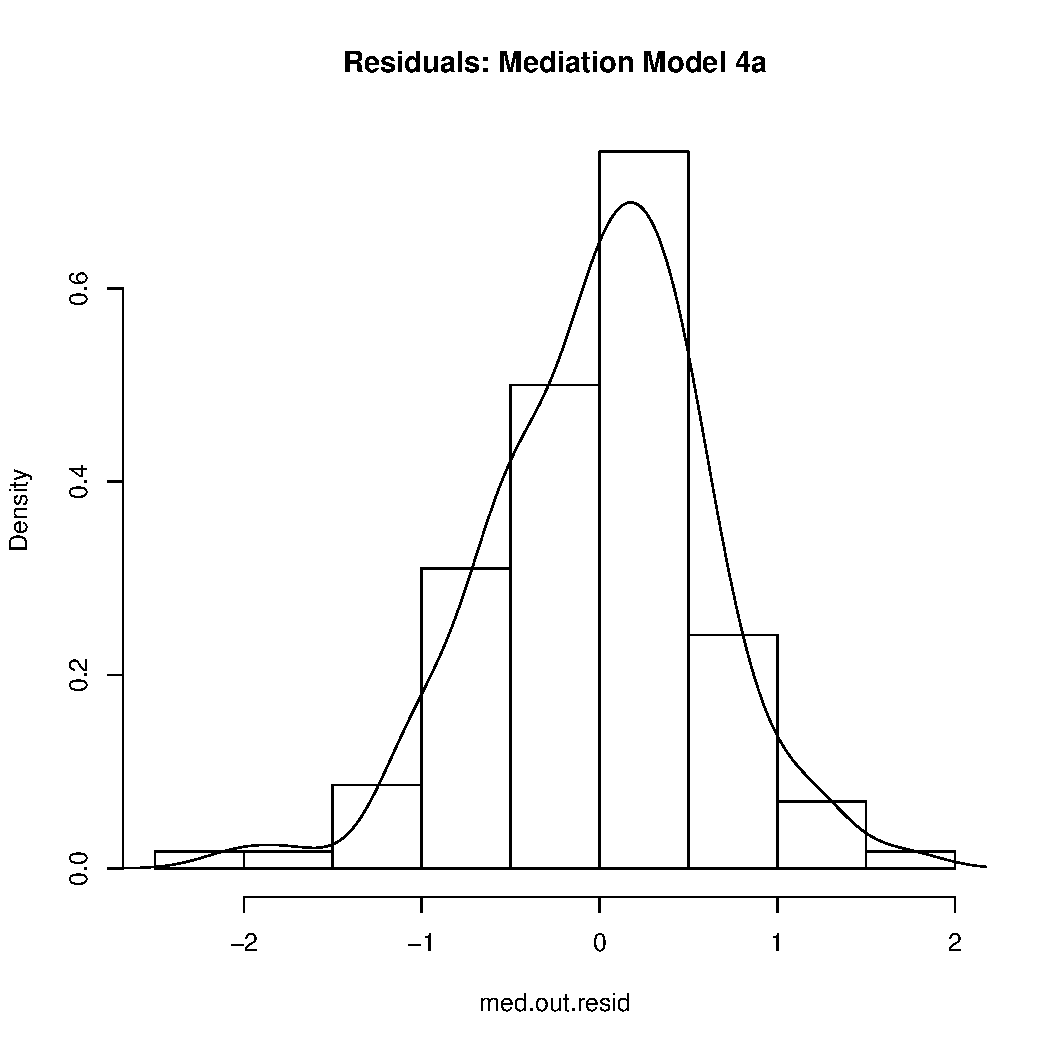
\includegraphics{finalDocuments/images/MLM4aResiduals.pdf}
%  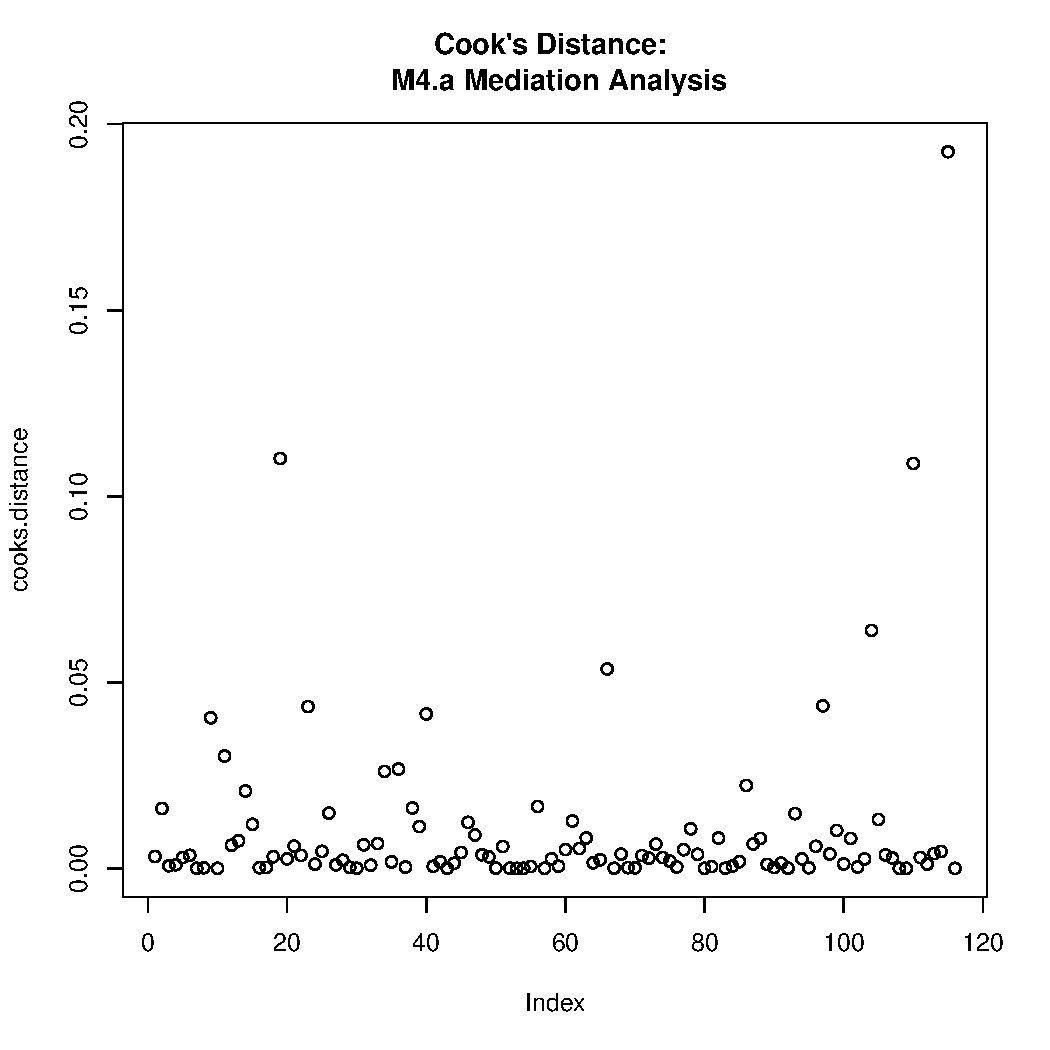
\includegraphics{finalDocuments/images/MLM4aCooksD.pdf}
%  \caption{M4a Mediation Analysis}
%  \label{fig:MLM4aAssumptions}
%\end{figure}

% (Baer et al 2006: 147) One method for constructing CIs assumes normality for the sampling distributions of the estimates. Under this assumption, 95% CIs for the average indirect effect and average total effect are obtained as Alternatively, one could perform a null hypothesis test by forming the critical ratio of each estimate to its standard error and comparing the result with the critical value of the z distribution. In andthe as- sumption of normality for the sampling distributions will not hold exactly, given that aˆb ˆ is a product of normally distributed estimates (and hence will not be normal). The deviation from normality may be small enough, however, that the CIs or significance tests will still be reasonably accurate.

%An alternative method for constructing CIs that may hold promise is the Monte Carlo (MC) method of MacKinnon et al. (2004). In this approach, the sampling distribution for the effect of interest is not assumed to be normal and is instead simulated from the model estimates and their asymptotic variances and covariances (a form of parametric bootstrap- ping). For instance, to simulate the sampling distribution of the average indirect effect, one would define a multinormal distribution with means equal to a ˆ, b ˆ, and ˆ aj ,bj and covariance matrix equal to the estimated covariance matrix of these estimates. One would then take random values from this multinormal distribution and plug them into Equation 5 to compute the average indirect effect. Collecting the results over many draws provides a simulated sampling distribution for the average indirect effect. One would then obtain conidence limits for the average indirect effect by taking the

%Preacher, K. J., & Selig, J. P. (2010, July). Monte Carlo method for assessing multilevel Mediation: An interactive tool for creating confidence intervals for indirect effects in 1-1-1 multilevel models [Computer software]. Available from http://quantpsy.org/.






\subsection{Discussion of Results: post-Tournament Analysis}
The results of the post-Tournament survey responses generally support predictions concerning the relationships between perceptions of joint action success, team click and social bonding.  The relationship between team performance expectations, team click, and social bonding, however, is less convincing.  Model 1.b, in which Team Performance Expectations predicts Team Click, while statistically significant, generates a very small beta coefficient.  Model 3.b, in which the relationship between Team Performance Expectations and Social Bonding, is not robust to model assumptions, and thus compromises the validity of the mediation analysis (model 4.b).  These results could suggest that while more positive violations of team performance expectations do contribute to feelings of Team Click, they might not contribute as strongly to feelings of social bonding.

Results show that, by contrast, perceived Joint Action Success is a strong predictor of both Team Click and Social bonding. Mediation analysis indicates that Team Click fully mediates the relationship between Joint Action Success and Social Bonding.


































\clearpage
\subsection{Analysis of pre-post Tournament data}
The predictions of the present study were further tested through an analysis of change in variables of interest between the pre- and post-Tournament surveys. By analysing pre- and post-Tournament responses, it was possible to investigate 1) to what extent variables of interest changed during the Tournament, and 2) whether pre-post changes in variables of interest were consistent with study predictions concerning the relationship between joint-action, team click, and social bonding.  When controlling for objective measures of success and feelings concerning individual performance, could change in social bonding be explained by changes in perceptions of joint-action success and/or changes in feelings of team click?




\subsubsection{Roadmap of pre-post Tournament Analysis}
Analysis of the pre-post Tournament data proceeded in the same manner as the post-Tournament data. The hypothesised relationship between joint-action success and social bonding was broken down into component relationships. \\

First, changes in feelings of team click were analysed as a function of changes in 1) perceptions of team component performance (Joint Action Success Pre Post), 2) post-Tournament appraisal of team performance relative to prior expectations (Team Performance Expectations), and 3) the interaction between these two predictor variables.
\bigskip
\begin{description}
  \item [Prediction 2.1.a] $\Delta$Joint Action Success  $\rightarrow$  $\Delta$Team Click
  \item [Prediction 2.1.b] $\Delta$Team Performance Expectations $\rightarrow$ $\Delta$ Team Click
  \item [Prediction 2.1.c] $\Delta$Joint Action Success $\rightarrow$ $\Delta$Team Click, moderated by $\Delta$Team Performance Expectations
\end{description}

Second, the change observed in social bonding (Social Bonding Pre Post) was analysed as a function of change in feelings of team click.
\bigskip
\begin{description}
  \item [Prediction 2.2.a] $\Delta$Team Click $\rightarrow$ $\Delta$Social Bonding
\end{description}

Third, the direct relationships between predictor variables (change in perceptions of join-action success and appraisal of team performance relative to prior expectation) and change in social bonding was analysed:
\bigskip
\begin{description}
  \item [Prediction 2.3.a] $\Delta$Joint Action Success $\rightarrow$ $\Delta$Social Bonding
  \item [Prediction 2.3.b] $\Delta$Team Performance Expectations $\rightarrow$ $\Delta$Social Bonding
\end{description}

Finally, a mediation analysis was performed to formally test whether feelings of team click mediated a direct relationship between perceptions of joint-action success and social bonding.

\begin{description}
  \item[Prediction 2.4.a Mediation Analysis] $\Delta$Joint Action Success $\rightarrow$ $\Delta$Team Click $\rightarrow$ $\Delta$Social Bonding
\end{description}

\clearpage


%\subsubsection{Pre-post Tournament Descriptive Analysis}








\subsubsection{Data Reduction}
As in the analysis of the post-Tournament survey responses, data reduction was performed on pre- and post-Tournament variables in order to consolidate measures of interest into underlying factors. The following results are extracted from EFAs using an oblique rotation method in R (see details above). In this analysis, pre- and post-Tournament responses for each collection of variables were combined in a single data frame, on which correlations between items and factor analysis was performed.  The variance of each factor over time was then analysed to assess whether there were meaningful changes.


\myparagraph{Component Performance for Individual and Team}
Survey items related to perceptions of component performance (team and individual) were collected and separately subjected to factor analysis (as in the post-Tournament analysis).

Correlations between team component performance items (team defence, team attack, team support play, and on field communication) were very high (all $r's > .65$), and the suitability of the correlation matrix for factor extraction was confirmed by relevant statistical tests ($KMO = 0.82$, corrtest Bartlett: $\chi^2(6, N = 238) = 717.55$, $p < .001$).  As such, one factor was imposed on items concerning team component performance, which explained 74.5\% of the overall variance in items relating to team performance (SS Loading = 2.97). $Guttman's \lambda =.90$ and $Cronbach's \alpha = (.92)$ indicated that the data reduction was appropriate.

Correlations between five items relating to individual performance (passing technique, support play in attack, 1on1 defence, and decision making in attack) were also sufficiently high (all $r's > .45$, $KMO = 0.83$, corrtest Bartlett: $\chi^2(10, N = 238) = 633.82$, $p < .001$), suggesting that one factor would be appropriate for individual performance (see Table ~\ref{X}).  One factor—``Ind Performance Success Pre Post''—was imposed, which explained 59.9\% of the overall variance (SS Loading = 2.99).  $Guttman's\lambda =.87$ and $Cronbach's \alpha = .88$ indicated that the data reduction was appropriate.


%$\chi^2 (df=2) = 20.27$, $p < .001$,
%$\chi^2 (df=5) = 47.29$, $p < .001$,

%To confirm that the theoretically motivated separation of Joint Action Success from Ind Performance Success was appropriate for the collected data, a follow up EFA was conducted, in which team and individual performance component variables were combined in one matrix. Sampling adequacy measures indicated high suitability ($KMO = 0.83$, $\chi^2(36, N = 118) = 726.60$, $p < .0001$).  As expected, an EFA extracted two factors, with Individual performance measures loaded on one factor (proportion of variance = .34, $SS Loading = 3.09$), and team performance measures loading on a second factor (proportion of variance = .32, $SS Loading = 2.90$). $Guttman's \lambda =.93$ and $Cronbach's \alpha = .90$ indicated that the data reduction was appropriate.



\myparagraph{Team Click}
Six survey items related to feelings of team click were collected and subjected to EFA. Correlations between variables was high, indicating that one factor was suitable (all $r's > .1$, $KMO = 0.78$, corrtest Bartlett: $\chi^2(15, N = 238) = 336.41$, $p < .001$).  One factor, ``Team Click Pre Post'', was imposed, which explained 37.6\% of the overall variance (all items loadings $> .4$, SS Loading = 2.26).  $Guttman's \lambda =.76$ and $Cronbach's \alpha = .76$ indicated that the data reduction was appropriate.
%$\chi^2(9, N = 238) = 31.52 $, $p < .001$

\myparagraph{Social Bonding}
Four survey items related to feelings of social bonding were subjected to EFA. Correlations between variables were generally high (all $r's > .3$, $KMO = 0.66$, corrtest Bartlett: $\chi^2(6, N = 238) = 218.95$, $p < .001$), indicating that one factor would be appropriate.  One factor, labelled ``Social Bonding Pre Post'' was extracted, which explained 41.9\% of the overall variance (SS Loading = 1.68).  $Guttman's \lambda =.68$ and $Cronbach's \alpha = .71$ indicated that the data reduction was appropriate.
% $\chi^2 (df=2) = 10.3 $, $p < .01$,

\myparagraph{Fatigue}
Three survey items related to feelings of fatigue  were collected and subjected to EFA.
Correlations between variables were high (all $r's > .55$, $KMO = .7$, corrtest Bartlett: $\chi^2(3, N = 238) = 382.88$, $p < .001$).  As such, one factor (``Fatigue Pre Post'') was imposed, which explained 66.3\% of the overall variance (SS Loading = 1.99).  $Guttman's \lambda =.8$ and $Cronbach's \alpha = .85$ indicated that the data reduction was appropriate.
%  $\chi^2(0, N = 238) = 0 $, $p < .001$,









\subsection{Pre-post Tournament Results}


\subsubsection{Pre-post Tournament differences in variables of interest}
Pre- and post-Tournament measures of variables of interest are displayed in tables below.  Three out of five variables designed to measure athletes' perceived success in components of individual performance appeared drop from pre- to post-Tournament (see Table ~\ref{tab:indPerformancePrePostSummary}).  Paired samples t-tests revealed significant negative mean differences between pre- and post-Tournament measures of passing technique ($M = -7.48 (-13.17, -1.80)$, $t(98)= -2.61,, p = .01$), support play ($M = -7.32 (-12.18, -2.47)$, $t(98)= -2.99,, p = .003$), and decision making in attack ($M = -5.19 ( -9.73, -0.65)$, $t(98)= -2.27,, p = .03$), while individual defence ($M = -3.42 (-9.01, 2.16)$, $t(98)= -1.22,, p = .23$), and effectiveness in contact ($M = -4.51 (-10.25, 1.24)$, $t(98)= -1.56,, p = .12$) did not decrease significantly between pre- and post-Tournament measures.

By contrast, all four variables designed to measure team success in components of joint-action did not differ significantly between pre- and post-Tournament measurements (see Table ~\ref{tab:teamPerformancePrePostSummary} for results).  Similarly, variables designed to measure team click also did not vary significantly.  These results suggest that athlete perceptions of team joint-action success and team click on average remained stable throughout the Tournament.  Perceptions of success in individual component performance, by contrast, decreased significantly, indicating that following the Tournament athletes were on average more critical of their performance following the Tournament.

In terms of Social Bonding, both feelings of emotional support and feelings of shared goal with the team differed significantly between pre- and post-Tournament measurements (see Table ~\ref{tab:bondingPrePostSummary}). Both measures increased significantly in the post-Tournament measure (emotional support: $M = 9.30 (4.16, 14.45)$, $t(98)= 3.59,, p = .0005$; shared goal $M = 7.12 (3.06, 11.19)$, $t(98)= 3.48,, p = .0007$).  All other variables did not vary significantly from pre-Tournament measures, except for the pictorial measure of fusion to \textit{family}, which increased significantly, $M = .33 (0.03, 0.64)$, $t(98)= 2.18, p = .03$.  Bonding variables for which measures were 5-point Likert may have suffered from ceiling effects: the mean and median of each Fusion Pictorial scale was $> 4$.  In general, it appeared that bonding to the team (and to one measure of Family) increased when measured following the Tournament.

In addition, variables designed to measure feelings of fatigue also varied significantly between pre- and post-Tournament measurements.  Fatigue ($M = 21.61 (15.02 28.20)$, $t(116)= 6.49,, p < .0001$), physical perceived exertion ($M = 2.84 (1.89, 3.79)$, $t(116)= 5.93, p < .0001$), and mental perceived exertion ($M = 2.84 (1.89, 3.79)$, $t(116)= 5.93, p < .0001$) all increased significantly from the point of first measurement immediately following the 2nd game on day 1 of the Tournament (see Table ~\ref{tab:fatiguePrePostSummary}).  Injury status post-Tournament did not differ significantly from pre-Tournament measures when tested using a paired-samples t-test, although the overall group mean difference between pre- and post-Tournament injury did show marginally significant signs of increasing, $M = 2.84 (-10.63, 0.59)$, $t(98)= 1.78, p = .08$.  These results indicate that on average, athletes felt higher levels of exertion and fatigue after the Tournament, than they did before or after the first game of the Tournament. This is to be expected, given the intensity of the rugby sevens Tournament format. It provides confirmation for the strenuous nature of the activity of the present study.


\subsubsection{Pre-post differences in latent factors}
Following data reduction, paired samples t-tests were used to compare pre- and post-Tournament measures of extracted factors relating to team and individual performance, team click, social bonding, and fatigue. Results are displayed in Table ~\ref{}.  Mean difference between athlete scores of team component performance (Joint Action Success Pre Post) did not vary significantly from pre- to post-Tournament, $M = -.06 (-0.30  0.18)$, $t(98)= -.48, p = .63$, nor did team click, $M = .06 (-0.12, 0.25)$, $t(98)= .69, p = .49$. Athlete mean differences in perceptions of components of individual performance (Ind Performance Success Pre Post) significantly decreased following the Tournament, $M = -0.28 (-0.47, -0.10)$, $t(98)= -2.99, p = .003$, suggesting that athletes were on average more critical of their individual performance than their team performance at the completion of the Tournament.

Tests revealed that the there was a significant difference in athlete reports of social bonding between pre- and post-Tournament measurements, $M = 0.34 (0.16, 0.52)$, $t(98)= 3.73, p = .0003$; Athletes' feelings of bonding on average increased from pre- to post-Tournament.  Average ratings of fatigue also significantly increased from measurement following athletes' second game on day 1 to ratings following the Tournament, $M =  0.77 (0.55, 0.99)$, $t(116)= 7.03, p < .0001$.


\clearpage


\newgeometry{margin=0.5cm} % modify this if you need even more space
\begin{landscape}

% Table created by stargazer v.5.2 by Marek Hlavac, Harvard University. E-mail: hlavac at fas.harvard.edu
% Date and time: Sun, Jun 25, 2017 - 22:44:09
\begin{table}[!htbp] \centering 
  \caption{Individual Performance change pre-post Tournament} 
  \label{tab:indPerformancePrePostSummary} 
\footnotesize 
\begin{tabular}{@{\extracolsep{5pt}} cccccccccc} 
\\[-1.8ex]\hline 
\hline \\[-1.8ex] 
 & Variable & Mean.pre & SD.pre & Mean.post & SD.post & MeanDiffernece & MeanPairedDifference & t-test & p-value \\ 
\hline \\[-1.8ex] 
1 & passingTechnique & $65.74$ & $24.94$ & $58.41$ & $24.25$ & $$-$7.33$ & $$-$7.48$ & $$-$2.61$ & $0.01$ \\ 
2 & supportPlay & $69.54$ & $23.23$ & $62.62$ & $22.70$ & $$-$6.92$ & $$-$7.32$ & $$-$2.99$ & $0.003$ \\ 
3 & individualDefense & $59.22$ & $26.64$ & $57.64$ & $23.57$ & $$-$1.57$ & $$-$3.42$ & $$-$1.22$ & $0.23$ \\ 
4 & effectivenessContact & $65.66$ & $24.85$ & $62.15$ & $24.81$ & $$-$3.51$ & $$-$4.51$ & $$-$1.56$ & $0.12$ \\ 
5 & decisionMakingAttack & $65.48$ & $23.80$ & $61.22$ & $21.43$ & $$-$4.26$ & $$-$5.19$ & $$-$2.27$ & $0.03$ \\ 
\hline \\[-1.8ex] 
\end{tabular} 
\end{table} 


% Table created by stargazer v.5.2 by Marek Hlavac, Harvard University. E-mail: hlavac at fas.harvard.edu
% Date and time: Sun, Jun 25, 2017 - 22:47:06
\begin{table}[!htbp] \centering 
  \caption{Team Performance change pre-post Tournament} 
  \label{tab:teamPerformancePrePostSummary} 
\footnotesize 
\begin{tabular}{@{\extracolsep{5pt}} cccccccccc} 
\\[-1.8ex]\hline 
\hline \\[-1.8ex] 
 & Variable & Mean.pre & SD.pre & Mean.post & SD.post & MeanDiffernece & MeanPairedDifference & t-test & p-value \\ 
\hline \\[-1.8ex] 
1 & teamDefense & $65.06$ & $22.85$ & $62.42$ & $22.50$ & $$-$2.63$ & $$-$4.92$ & $$-$1.57$ & $0.12$ \\ 
2 & teamAttack & $66.01$ & $24.95$ & $65.33$ & $20.26$ & $$-$0.68$ & $$-$1.59$ & $$-$0.55$ & $0.58$ \\ 
3 & teamSupportPlay & $64.36$ & $23.53$ & $65.75$ & $19.72$ & $1.40$ & $0.90$ & $0.35$ & $0.73$ \\ 
4 & teamCommunication & $62.37$ & $24.21$ & $65.25$ & $21.26$ & $2.89$ & $$-$0.07$ & $$-$0.03$ & $0.98$ \\ 
\hline \\[-1.8ex] 
\end{tabular} 
\end{table} 


% Table created by stargazer v.5.2 by Marek Hlavac, Harvard University. E-mail: hlavac at fas.harvard.edu
% Date and time: Sat, Jun 03, 2017 - 15:44:29
\begin{table}[!htbp] \centering 
  \caption{click change pre-post Tournament} 
  \label{} 
\footnotesize 
\begin{tabular}{@{\extracolsep{5pt}} cccccccccc} 
\\[-1.8ex]\hline 
\hline \\[-1.8ex] 
 & Variable & Mean.pre & SD.pre & Mean.post & SD.post & MeanDiffernece & MeanPairedDifference & t-test & p-value \\ 
\hline \\[-1.8ex] 
1 & unspokenUnderstanding & $71.58$ & $20.77$ & $72.72$ & $19.95$ & $1.14$ & $1.33$ & $0.58$ & $0.56$ \\ 
2 & generalAtmosphere & $75.51$ & $23.27$ & $78.45$ & $21.34$ & $2.94$ & $1.05$ & $0.47$ & $0.64$ \\ 
3 & clickPictorial & $3.87$ & $1.24$ & $3.93$ & $1.04$ & $0.07$ & $0.03$ & $0.21$ & $0.84$ \\ 
4 & reliabilityOfOthers & $67.43$ & $28.01$ & $68$ & $23.09$ & $0.57$ & $1.21$ & $0.40$ & $0.69$ \\ 
5 & reliabilityForOthers & $62.38$ & $25.40$ & $63.45$ & $25.80$ & $1.07$ & $1.06$ & $0.38$ & $0.70$ \\ 
6 & abilityExtended & $70.45$ & $25.83$ & $72.25$ & $19.27$ & $1.80$ & $1.43$ & $0.53$ & $0.60$ \\ 
\hline \\[-1.8ex] 
\end{tabular} 
\end{table} 


% Table created by stargazer v.5.2 by Marek Hlavac, Harvard University. E-mail: hlavac at fas.harvard.edu
% Date and time: Sun, Jun 25, 2017 - 22:51:01
\begin{table}[!htbp] \centering 
  \caption{bonding change pre-post Tournament} 
  \label{tab:bondingPrePostSummary} 
\footnotesize 
\begin{tabular}{@{\extracolsep{5pt}} cccccccccc} 
\\[-1.8ex]\hline 
\hline \\[-1.8ex] 
 & Variable & Mean.pre & SD.pre & Mean.post & SD.post & MeanDiffernece & MeanPairedDifference & t-test & p-value \\ 
\hline \\[-1.8ex] 
1 & emotionalSupport & $70.12$ & $26.21$ & $79.67$ & $18.84$ & $9.55$ & $9.30$ & $3.59$ & $0.001$ \\ 
2 & sharedGoal & $77.66$ & $24.28$ & $86$ & $15.56$ & $8.34$ & $7.12$ & $3.48$ & $0.001$ \\ 
3 & groupId & $4.34$ & $0.78$ & $4.29$ & $0.67$ & $$-$0.04$ & $0.06$ & $0.78$ & $0.44$ \\ 
4 & fusionVerbal & $4.03$ & $0.74$ & $4.00$ & $0.71$ & $$-$0.03$ & $0$ & $0$ & $1$ \\ 
5 & fusionPictorialTeam & $4.26$ & $1.25$ & $4.33$ & $1.19$ & $0.07$ & $0.04$ & $0.30$ & $0.77$ \\ 
6 & fusionPictorialCountry & $4.01$ & $1.58$ & $4.03$ & $1.39$ & $0.02$ & $$-$0.04$ & $$-$0.22$ & $0.83$ \\ 
7 & fusionPictorialFamily & $4.10$ & $1.50$ & $4.51$ & $0.96$ & $0.41$ & $0.33$ & $2.18$ & $0.03$ \\ 
8 & rankTeam & $1.49$ & $0.79$ & $1.61$ & $0.81$ & $0.12$ & $0.09$ & $1.15$ & $0.25$ \\ 
9 & rankCountry & $1.92$ & $1.06$ & $1.93$ & $1.03$ & $$ & $$-$0.04$ & $$-$0.44$ & $0.66$ \\ 
10 & rankFamily & $1.41$ & $0.88$ & $1.42$ & $0.86$ & $0.01$ & $0$ & $0$ & $1$ \\ 
\hline \\[-1.8ex] 
\end{tabular} 
\end{table} 


% Table created by stargazer v.5.2 by Marek Hlavac, Harvard University. E-mail: hlavac at fas.harvard.edu
% Date and time: Sun, Jun 25, 2017 - 23:08:36
\begin{table}[!htbp] \centering 
  \caption{Fatigue change pre-post Tournament} 
  \label{fatiguePrePostSummary} 
\footnotesize 
\begin{tabular}{@{\extracolsep{5pt}} cccccccccc} 
\\[-1.8ex]\hline 
\hline \\[-1.8ex] 
 & Variable & Mean.pre & SD.pre & Mean.post & SD.post & MeanDiffernece & MeanPairedDifference & t-test & p-value \\ 
\hline \\[-1.8ex] 
1 & fatigue & $50.14$ & $28.80$ & $69.27$ & $21.24$ & $19.13$ & $21.61$ & $6.49$ & $0$ \\ 
2 & prpe & $12.45$ & $4.52$ & $14.97$ & $2.66$ & $2.52$ & $2.84$ & $5.93$ & $0.0000$ \\ 
3 & mental & $4.09$ & $2.83$ & $6.08$ & $2.47$ & $1.99$ & $2.30$ & $6.85$ & $0$ \\ 
4 & injury & $81.28$ & $23.36$ & $76.14$ & $26.91$ & $$-$5.13$ & $5.02$ & $1.78$ & $0.08$ \\ 
\hline \\[-1.8ex] 
\end{tabular} 
\end{table} 


% Table created by stargazer v.5.2 by Marek Hlavac, Harvard University. E-mail: hlavac at fas.harvard.edu
% Date and time: Sat, Jun 03, 2017 - 17:41:41
\begin{table}[!htbp] \centering 
  \caption{factors change pre-post Tournament} 
  \label{} 
\footnotesize 
\begin{tabular}{@{\extracolsep{5pt}} cccccccccc} 
\\[-1.8ex]\hline 
\hline \\[-1.8ex] 
 & Variable & Mean.pre & SD.pre & Mean.post & SD.post & MeanDiffernece & MeanPairedDifference & t-test & p-value \\ 
\hline \\[-1.8ex] 
1 & teamPerformanceFactorPrePost & $$-$0.01$ & $1.04$ & $0.01$ & $0.88$ & $0.01$ & $$-$0.06$ & $$-$0.48$ & $0.63$ \\ 
2 & indPerformanceFactorPrePost & $0.12$ & $0.95$ & $$-$0.13$ & $0.93$ & $$-$0.25$ & $$-$0.28$ & $$-$2.99$ & $0.004$ \\ 
3 & clickFactorPrePost & $$-$0.04$ & $0.98$ & $0.04$ & $0.85$ & $0.09$ & $0.06$ & $0.69$ & $0.84$ \\ 
4 & bondingFactorPrePost & $$-$0.18$ & $1.03$ & $0.19$ & $0.71$ & $0.37$ & $0.34$ & $3.74$ & $0.0003$ \\ 
5 & fatigueFactorPrePost & $$-$0.29$ & $1.01$ & $0.40$ & $0.65$ & $0.68$ & $0.77$ & $7.03$ & $0$ \\ 
\hline \\[-1.8ex] 
\end{tabular} 
\end{table} 

\end{landscape}
\restoregeometry



\subsection{Model Selection}
The statistics outlined above suggested that further analysis into the relationships between changing variables was appropriate. The number of observations available in the pre-post Tournament data were insufficient to construct a mixed-effects repeated measures design in which both the intercept and slope of observations could vary according to each individual athlete nested within their given team over time.\footnote{Allowing both the intercept and slope to vary requires twice the number of observations to estimate the random effects ($2x174 = 248$), whereas the available number of observations was only 198} Alternative models for suitable for repeated measures designs, such as RM-ANOVA or ANCOVA, are also incapable of allowing each fixed factor (the regression coefficient or slope) to vary randomly according to higher level factors (individual and team), and are also unable to handle unbalanced designs (in this case, due missing data for athletes across pre- and post-Tournament measurements). As a compromise, change scores in variables of interest (individual and team performance, team click, social bonding, and fatigue) were calculated by subtracting pre- from post-Tournament scores for each athlete. The calculation of change scores reduced the complexity of the data structure down to two levels of analysis, and meant that relationships between these change variables could be modelled using a linear mixed effects regression. Change scores of relevant factors were introduced to the model as fixed effects, and their slopes and intercepts were allowed to vary according to team.


\subsubsection{2.1.a $\Delta$Team Click $\sim$ $\Delta$Joint Action Success}
The first step was to test the prediction that a change in team click could be related to changes in athlete perception of joint-action success. Controlling for Tournament performance, measures and objective and subjective competence (fixed effects), and team-level variance (random effect), the model revealed a significant positive relationship between change in perceptions of joint-action success and change in feelings of team click, $\beta = .52$ ($95\% CI =  .34, .71$), $SE = 0.09$, $t(11.32) = 5.55$, $p < .001$, $marginal R^2 = .40$, $conditional R^2 = .47$ (see Table ~\ref{tab:MLM21aJointActionSuccesscClick} for results of all iterations of the model).  Model residuals were normally distributed around zero ($W = 0.98228, p = .22$), and individual cases had low influence on the model (Cook's Distances all < .20, see Appendix Figure \ref{fig:MLM21aAssumptions}).  This model supported the prediction that more positive perceptions of joint-action success correlate with stronger feelings of team click, by showing that athletes who experienced a positive increase in perceptions of joint-action success also reported a positive increase in feelings of team click throughout the Tournament.


% Table created by stargazer v.5.2 by Marek Hlavac, Harvard University. E-mail: hlavac at fas.harvard.edu
% Date and time: Tue, Jun 27, 2017 - 09:10:21
\begin{table}[!htbp] \centering 
  \caption{cTeamClick ~ cJointActionSuccess} 
  \label{tab:MLM21aJointActionSuccesscClick} 
\begin{tabular}{@{\extracolsep{5pt}}lccc} 
\\[-1.8ex]\hline 
\hline \\[-1.8ex] 
 & \multicolumn{3}{c}{\textit{Dependent variable:}} \\ 
\cline{2-4} 
\\[-1.8ex] & \multicolumn{3}{c}{cTeamClick} \\ 
\\[-1.8ex] & (1) & (2) & (3)\\ 
\hline \\[-1.8ex] 
 (constant) & 0.10 & 0.10 & $-$0.10 \\ 
  & (0.13) & (0.08) & (0.28) \\ 
  & & & \\ 
 cJointActionSuccess &  & 0.47$^{***}$ & 0.52$^{***}$ \\ 
  &  & (0.08) & (0.09) \\ 
  & & & \\ 
 cIndPerformanceSuccess &  &  & $-$0.04 \\ 
  &  &  & (0.09) \\ 
  & & & \\ 
 objectiveCompetence &  &  & 0.03 \\ 
  &  &  & (0.09) \\ 
  & & & \\ 
 subjectiveCompetence &  &  & $-$0.01 \\ 
  &  &  & (0.08) \\ 
  & & & \\ 
 finalRank &  &  & $-$0.02 \\ 
  &  &  & (0.04) \\ 
  & & & \\ 
 minutesTotal &  &  & 0.004 \\ 
  &  &  & (0.004) \\ 
  & & & \\ 
 pointsTotal &  &  & 0.01 \\ 
  &  &  & (0.01) \\ 
  & & & \\ 
\hline \\[-1.8ex] 
Marginal R-squared &  &  & .40 \\ 
Conditional R-squared &  &  & .47 \\ 
Observations & 99 & 99 & 97 \\ 
Log Likelihood & $-$130.59 & $-$107.75 & $-$104.44 \\ 
Akaike Inf. Crit. & 267.19 & 227.50 & 232.88 \\ 
Bayesian Inf. Crit. & 274.97 & 243.07 & 263.77 \\ 
\hline 
\hline \\[-1.8ex] 
\textit{Note:}  & \multicolumn{3}{r}{$^{*}$p$<$0.05; $^{**}$p$<$0.01; $^{***}$p$<$0.001} \\ 
\end{tabular} 
\end{table} 






\subsubsection{2.1.b $\Delta$Team Click $\sim$ Team Performance Expectations}

The relationship between team performance relative to prior expectations (recorded following the Tournament) and Team Click was analysed. The model revealed a significant positive relationship between Team Performance Expectations and change in Team Click,  $\beta = .27$ ($95\% CI =  .05, .49$), $SE = 0.11$, $t(32.97) = 2.36$, $p = .02$, $marginal R^2 = .12$, $conditional R^2 = .22$, indicating that athletes who were more positive about their appraisals of team performance following the Tournament on average experienced an increase in feelings of team click.

Examination of model residuals revealed that they were not normally distributed around zero ($W = 0.95, p = .001$), due to positive skew ($.85$) (see Appendix Figure ~\ref{fig:MLM21bAssumptions}).  Log-transformation of the outcome variable did not markedly improve the non-normality of residuals, ($Shapiro-Wilk = 0.96, p = .008$).  Instead, exclusion of outliers according to Tukey's method improved the model fit such that residuals were normally distributed, ($Shapiro-Wilk = 0.99, p = .72$), and individual cases had low influence on the model (Cook's Distances all < .10, see Appendix Figure ~\ref{fig:MLM21bOutAssumptions}).
The adjusted model supported the original significant positive effect of Team Performance Expectations on Team Click, $\beta = .36$ ($95\% CI =  .16, .55$), $SE = 0.10$, $t(9.78) = 3.66$, $p < .01$, $marginal R^2 = .16$, $conditional R^2 = .55$.  See Table ~\ref{tab:MLM21bOutLogComparison} for a comparison of adjusted models. These results confirm the prediction that those who experience more positive violations around team performance also experience an higher levels of Team Click---shown in this case by an increase in feelings of Team Click between pre- and post-Tournament measurements.


%The adjusted model also revealed a significant negative effect of violations of expectations around \textit{individual} performance on team click, $\beta = -.008 (95\% CI =  -.01, .001), SE = 0.004, t(91.79) = -2.28, p = .03$,  which could suggest that athletes who experienced more positive violations about their own performance did not feel the team click as strongly.


% Table created by stargazer v.5.2 by Marek Hlavac, Harvard University. E-mail: hlavac at fas.harvard.edu
% Date and time: Tue, Jun 27, 2017 - 09:21:13
\begin{table}[!htbp] \centering 
  \caption{M2.1b cTeamClick ~ cPerformanceExpectations} 
  \label{tab:MLM21bcTeamPerfExpcClick} 
\begin{tabular}{@{\extracolsep{5pt}}lccc} 
\\[-1.8ex]\hline 
\hline \\[-1.8ex] 
 & \multicolumn{3}{c}{\textit{Dependent variable:}} \\ 
\cline{2-4} 
\\[-1.8ex] & \multicolumn{3}{c}{cTeamClick} \\ 
\\[-1.8ex] & (1) & (2) & (3)\\ 
\hline \\[-1.8ex] 
 (constant) & 0.10 & $-$0.57 & $-$0.64 \\ 
  & (0.13) & (0.30) & (0.44) \\ 
  & & & \\ 
 cTeamPerformanceExpectations &  & 0.01$^{*}$ & 0.01$^{*}$ \\ 
  &  & (0.004) & (0.005) \\ 
  & & & \\ 
 cIndPerformanceExpectations &  &  & $-$0.003 \\ 
  &  &  & (0.004) \\ 
  & & & \\ 
 objectiveCompetence &  &  & $-$0.13 \\ 
  &  &  & (0.11) \\ 
  & & & \\ 
 subjectiveCompetence &  &  & $-$0.16 \\ 
  &  &  & (0.09) \\ 
  & & & \\ 
 finalRank &  &  & 0.02 \\ 
  &  &  & (0.06) \\ 
  & & & \\ 
 minutesTotal &  &  & 0.003 \\ 
  &  &  & (0.005) \\ 
  & & & \\ 
 pointsTotal &  &  & 0.003 \\ 
  &  &  & (0.01) \\ 
  & & & \\ 
\hline \\[-1.8ex] 
Marginal R-squared &  &  & .40 \\ 
Conditional R-squared &  &  & .47 \\ 
Observations & 99 & 99 & 97 \\ 
Log Likelihood & $-$130.59 & $-$127.00 & $-$123.15 \\ 
Akaike Inf. Crit. & 267.19 & 266.01 & 270.30 \\ 
Bayesian Inf. Crit. & 274.97 & 281.58 & 301.20 \\ 
\hline 
\hline \\[-1.8ex] 
\textit{Note:}  & \multicolumn{3}{r}{$^{*}$p$<$0.05; $^{**}$p$<$0.01; $^{***}$p$<$0.001} \\ 
\end{tabular} 
\end{table} 


\begin{table}
\begin{center}
\begin{tabular}{l c c c }
\toprule
 & Controls & Log-adjusted & Outliers removed \\
\midrule
(constant)                                 & $0.33$               & $\mathbf{1.27}^{***}$ & $0.40$                \\
                                           & $(0.51)$             & $(0.16)$              & $(0.39)$              \\
Team Performance Vs Expectations           & $\mathbf{0.30}^{**}$ & $\mathbf{0.09}^{*}$   & $\mathbf{0.32}^{***}$ \\
                                           & $(0.11)$             & $(0.04)$              & $(0.08)$              \\
Ind Performance Vs Expectations            & $-0.10$              & $-0.03$               & $\mathbf{-0.22}^{**}$ \\
                                           & $(0.10)$             & $(0.03)$              & $(0.08)$              \\
Objective Competence                       & $-0.15$              & $-0.05$               & $0.03$                \\
                                           & $(0.12)$             & $(0.04)$              & $(0.10)$              \\
Subjective Competence                      & $-0.15$              & $-0.05$               & $-0.03$               \\
                                           & $(0.09)$             & $(0.03)$              & $(0.08)$              \\
Final Rank                                 & $-0.01$              & $-0.00$               & $-0.08$               \\
                                           & $(0.06)$             & $(0.02)$              & $(0.04)$              \\
Minutes Total                              & $0.00$               & $0.00$                & $-0.00$               \\
                                           & $(0.01)$             & $(0.00)$              & $(0.00)$              \\
Points Total                               & $0.00$               & $0.00$                & $0.01$                \\
                                           & $(0.01)$             & $(0.00)$              & $(0.01)$              \\
Fatigue                                    & $-0.08$              & $-0.00$               & $-0.07$               \\
                                           & $(0.11)$             & $(0.04)$              & $(0.09)$              \\
Extraverted                                & $-0.06$              & $-0.02$               & $0.01$                \\
                                           & $(0.07)$             & $(0.02)$              & $(0.05)$              \\
\midrule
AIC                                        & 253.92               & 50.47                 & 200.30                \\
BIC                                        & 288.92               & 85.47                 & 234.66                \\
Log Likelihood                             & -112.96              & -11.23                & -86.15                \\
Num. obs.                                  & 90                   & 90                    & 86                    \\
Num. groups: team                          & 13                   & 13                    & 13                    \\

\bottomrule
\multicolumn{4}{l}{\scriptsize{Coefficients with $p < 0.05$ in \textbf{bold}. Effect size of model excluding outliers: Marginal $R^2 = .17$, Conditional $R^2 = .20$}}
\end{tabular}
\caption{Prediction 2: Team Click Change predicts Social Bonding Change in the Post-Tournament survey data (n = 90).}
\label{tab:MLM21bOutLogComparison}
\end{center}
\end{table}



%Low values for both of these regression coefficients...


\subsubsection{2.1.c $\Delta$Team Click $\sim$ $\Delta$Joint Action Success$\times$ Team Performance Expectations}
Introduction of the interaction effect of change in perceptions of joint-action success and expectations around team performance on Team Click was not significant, $\beta = .004$ ($95\% CI =  -.002, .01$), $SE = 0.003$, $t(30.14) = 1.42$, $p = .17$, $marginal R^2 = .40$, $conditional R^2 = .49$, and failed to improve the model fit, $\chi^2 = 2.72$, $ p = .44$ (see Table ~\ref{tab:MLM21ccTeamPerfExpcClickInt}).  This result indicates that the extent to which team performance violations were more or less positive did not have an additive effect on the positive relationship between perceptions of Joint Action Success and Team Click.



\subsubsection{2.2.a $\Delta$Social Bonding$\sim$ $\Delta$Team Click}
Next, the change in social bonding observed pre- to post-Tournament was analysed as a function of change in feelings of team click.  The model revealed a significant positive effect of change in team click on change in social bonding, $\beta = .40$ ($95\% CI =  .16, .64$), $SE = .12$, $t(7.02) = 3.31$, $p = .01$, $marginal R^2 = .17$, $conditional R^2 = .23$ (see Table ~\ref{tab:MLM22acClickcBonding} for a full description of model estimates).  Model residuals were normally distributed around zero ($Shapiro-Wilk = 0.98, p = .15$). and individual cases had low influence on the model (Cook's Distances all < .6, see Appendix Figure ~\ref{fig:MLM22aAssumptions} for details). This model suggests that athletes who experienced an increase in feelings of team click also experienced an increase in feelings of social bonding towards their team.



\begin{table}
\begin{center}
\begin{tabular}{l c c c }
\toprule
 & Intercept & Main effect & Controls \\
\midrule
(constant)                                     & $\mathbf{0.34}^{***}$ & $\mathbf{0.31}^{***}$ & $0.29$               \\
                                               & $(0.09)$              & $(0.08)$              & $(0.46)$             \\
Team Click Change                              &                       & $\mathbf{0.39}^{***}$ & $\mathbf{0.37}^{**}$ \\
                                               &                       & $(0.11)$              & $(0.14)$             \\
Objective Competence                           &                       &                       & $0.08$               \\
                                               &                       &                       & $(0.10)$             \\
Subjective Competence                          &                       &                       & $0.01$               \\
                                               &                       &                       & $(0.09)$             \\
Final Rank                                     &                       &                       & $0.00$               \\
                                               &                       &                       & $(0.05)$             \\
Minutes Total                                  &                       &                       & $0.01$               \\
                                               &                       &                       & $(0.00)$             \\
Points Total                                   &                       &                       & $0.00$               \\
                                               &                       &                       & $(0.01)$             \\
Fatigue                                        &                       &                       & $-0.09$              \\
                                               &                       &                       & $(0.10)$             \\
Extraverted                                    &                       &                       & $-0.03$              \\
                                               &                       &                       & $(0.06)$             \\
\midrule
AIC                                            & 265.55                & 256.54                & 241.81               \\
BIC                                            & 273.34                & 272.11                & 274.31               \\
Log Likelihood                                 & -129.78               & -122.27               & -107.90              \\
Num. obs.                                      & 99                    & 99                    & 90                   \\
Num. groups: team                              & 14                    & 14                    & 13                   \\
\bottomrule
\multicolumn{4}{l}{\scriptsize{Coefficients with $p < 0.05$ in \textbf{bold}. Marginal $R^2 = .17$, Conditional $R^2 = .23$}}
\end{tabular}
\caption{Prediction 2: Team Click Change predicts Social Bonding Change in the Post-Tournament survey data (n = 90).}
\label{tab:MLM22acClickcBonding}
\end{center}
\end{table}





%Exclusion of outliers according to Tukey's method (observations above and below 1.5 \times Inter Quartile Range (IQR)) appeared to improve the model fit, $\beta = .25$ ($95\% CI =  .11, .48$), $SE = .10$, $t(6.58) = 3.06$, $p < .02$, $marginal R^2 = .18$, $conditional R^2 = .25$. Model residuals were normally distributed, ($Shapiro-Wilk = 0.98, p = .14$),




\subsubsection{2.3.a $\Delta$Social Bonding $\sim$ $\Delta$Joint Action Success}
Next, change in social bonding pre-post Tournament as a function of change in Joint Action Success was tested. Results of the model revealed a significant positive effect of change in Joint Action Success on changes in Social Bonding, $\beta = .38$ ($95\% CI =  .21, .56$), $SE = .09$, $t(97) = 4.35$, $p < .0001$, $marginal R^2 = .18$, $conditional R^2 = .18$, suggesting that on average, athletes who experienced an increase in positive perceptions of joint-action success as a result of the Tournament also experienced an increase in feelings of bondedness to their team.  Interestingly, the model also revealed a significant \textit{negative} effect of perceptions of success in individual component performance and social bonding, $\beta = -.23$ ($95\% CI =  -.44, -.02$), $SE = .11$, $t(97) = -2.12$, $p = .04$, indicating that athletes who's attitudes towards their own performance increased in positivity showed an average decrease in feelings of social bonding between pre- and post-Tournament measures. All other fixed effects were not significant, see Table ~\ref{tab:MLM23acJointActionSuccesscBonding}. Model residuals were normally distributed around zero ($W = 0.98, p = .19$), and individual cases had low influence on the model (Cook's Distances all < .5, see Appendix Figure ~\ref{fig:MLM23aAssumptions}.  This model supported the prediction that higher perceptions of joint action success would significantly relate to higher levels of social bonding, by showing that increases in perception of joint action success significantly predicted increases in feelings of social bonding before and after the Tournament.



% Table created by stargazer v.5.2 by Marek Hlavac, Harvard University. E-mail: hlavac at fas.harvard.edu
% Date and time: Tue, Jun 27, 2017 - 17:13:12
\begin{table}[!htbp] \centering 
  \caption{cSocialBonding ~ cJointActionSuccess} 
  \label{tab:MLM23acJointActionSuccesscBonding} 
\footnotesize 
\begin{tabular}{@{\extracolsep{5pt}}lccc} 
\\[-1.8ex]\hline 
\hline \\[-1.8ex] 
 & \multicolumn{3}{c}{\textit{Dependent variable:}} \\ 
\cline{2-4} 
\\[-1.8ex] & \multicolumn{3}{c}{cSocialBonding} \\ 
\\[-1.8ex] & (1) & (2) & (3)\\ 
\hline \\[-1.8ex] 
 (constant) & 0.34$^{***}$ & 0.35$^{***}$ & 0.13 \\ 
  & (0.09) & (0.09) & (0.31) \\ 
  & & & \\ 
 cJointActionSuccess &  & 0.24$^{***}$ & 0.38$^{***}$ \\ 
  &  & (0.07) & (0.09) \\ 
  & & & \\ 
 cIndPerformanceSuccess &  &  & $-$0.23$^{*}$ \\ 
  &  &  & (0.11) \\ 
  & & & \\ 
 objectiveCompetence &  &  & 0.14 \\ 
  &  &  & (0.11) \\ 
  & & & \\ 
 subjectiveCompetence &  &  & 0.03 \\ 
  &  &  & (0.09) \\ 
  & & & \\ 
 finalRank &  &  & $-$0.04 \\ 
  &  &  & (0.05) \\ 
  & & & \\ 
 minutesTotal &  &  & 0.01 \\ 
  &  &  & (0.005) \\ 
  & & & \\ 
 pointsTotal &  &  & 0.003 \\ 
  &  &  & (0.01) \\ 
  & & & \\ 
\hline \\[-1.8ex] 
Marginal R-squared &  & .10 & .18 \\ 
Conditional R-squared &  & .10 & .18 \\ 
Observations & 99 & 99 & 97 \\ 
Log Likelihood & $-$129.78 & $-$124.37 & $-$118.30 \\ 
Akaike Inf. Crit. & 265.55 & 260.75 & 260.60 \\ 
Bayesian Inf. Crit. & 273.34 & 276.32 & 291.50 \\ 
\hline 
\hline \\[-1.8ex] 
\textit{Note:}  & \multicolumn{3}{r}{$^{*}$p$<$0.05; $^{**}$p$<$0.01; $^{***}$p$<$0.001} \\ 
\end{tabular} 
\end{table} 





\subsubsection{2.3.b $\Delta$Social Bonding $\sim$ Team Performance Expectations}
A model designed to test the relationship between expectations around team performance and change in social bonding revealed a marginally significant main effect, $\beta = .20$ ($95\% CI =  -.0004, .02$), $SE = .11$, $t(97) = 1.87$, $p = .07$, $marginal R^2 = .05$, $conditional R^2 = .05$.  Examination of model residuals revealed that they were not normally distributed around zero ($Shapiro-Wilk = 0.96, p = .004$).

Re-running the model with a log-transformed outcome variable and outliers excluded improved the normality of residuals, ($Shapiro-Wilk = 0.98, p = .24$), however the effect of Team Performance Expectations on Social Bonding was no longer significant, $\beta = .04$ ($95\% CI =  .02, .10$), $SE = .03$, $t()) = 1.29$, $p = .01$, $marginal R^2 = .03$, $conditional R^2 = .09$ (see Table ~\ref{tab:MLM23bcBondingteamPerfExp} for full description of results).  These results from adjusted models suggests that variation in Team Performance Expectations across pre- and post-Tournament measurements did not suitably explain observed variation in pre-post measures of Social Bonding.  As such, Team Performance Expectations was not considered in the subsequent mediation analysis.



\newgeometry{margin=0.5cm}

% Table created by stargazer v.5.2 by Marek Hlavac, Harvard University. E-mail: hlavac at fas.harvard.edu
% Date and time: Tue, Jun 27, 2017 - 17:15:15
\begin{table}[!htbp] \centering 
  \caption{cSocialBonding ~ teamPerformanceExpectations} 
  \label{tab:MLM23bcBondingteamPerfExp} 
\scriptsize 
\begin{tabular}{@{\extracolsep{5pt}}lccccc} 
\\[-1.8ex]\hline 
\hline \\[-1.8ex] 
 & \multicolumn{5}{c}{\textit{Dependent variable:}} \\ 
\cline{2-6} 
\\[-1.8ex] & \multicolumn{3}{c}{cSocialBonding} & bondingPostFactorLogReturned & bondingFactorChangePrePostOut \\ 
\\[-1.8ex] & (1) & (2) & (3) & (4) & (5)\\ 
\hline \\[-1.8ex] 
 (constant) & 0.34$^{***}$ & $-$0.07 & 0.01 & 1.34$^{***}$ & $-$0.01 \\ 
  & (0.09) & (0.25) & (0.39) & (0.22) & (0.33) \\ 
  & & & & & \\ 
 teamPerformanceExpectations &  & 0.01$^{*}$ & 0.01$^{*}$ & 0.01$^{***}$ & 0.005 \\ 
  &  & (0.004) & (0.004) & (0.003) & (0.004) \\ 
  & & & & & \\ 
 indPerformanceExpectations &  &  & $-$0.004 & 0.001 & $-$0.0000 \\ 
  &  &  & (0.004) & (0.002) & (0.003) \\ 
  & & & & & \\ 
 objectiveCompetence &  &  & 0.03 & 0.01 & 0.04 \\ 
  &  &  & (0.11) & (0.04) & (0.08) \\ 
  & & & & & \\ 
 subjectiveCompetence &  &  & $-$0.06 & 0.09$^{**}$ & $-$0.03 \\ 
  &  &  & (0.10) & (0.04) & (0.07) \\ 
  & & & & & \\ 
 finalRank &  &  & $-$0.03 & 0.01 & $-$0.03 \\ 
  &  &  & (0.05) & (0.02) & (0.04) \\ 
  & & & & & \\ 
 minutesTotal &  &  & 0.004 & 0.0003 & 0.001 \\ 
  &  &  & (0.005) & (0.002) & (0.003) \\ 
  & & & & & \\ 
 pointsTotal &  &  & 0.002 & $-$0.002 & $-$0.0003 \\ 
  &  &  & (0.01) & (0.003) & (0.01) \\ 
  & & & & & \\ 
\hline \\[-1.8ex] 
Marginal R-squared &  & .03 & .05 & .23 &  \\ 
Conditional R-squared &  & .03 & .05 & .46 &  \\ 
Observations & 99 & 99 & 97 & 97 & 86 \\ 
Log Likelihood & $-$129.78 & $-$128.30 & $-$125.20 & $-$32.67 & $-$75.13 \\ 
Akaike Inf. Crit. & 265.55 & 268.60 & 274.39 & 89.34 & 174.25 \\ 
Bayesian Inf. Crit. & 273.34 & 284.17 & 305.29 & 120.24 & 203.70 \\ 
\hline 
\hline \\[-1.8ex] 
\textit{Note:}  & \multicolumn{5}{r}{$^{*}$p$<$0.1; $^{**}$p$<$0.05; $^{***}$p$<$0.01} \\ 
\end{tabular} 
\end{table} 

% Table created by stargazer v.5.2 by Marek Hlavac, Harvard University. E-mail: hlavac at fas.harvard.edu
% Date and time: Tue, Jun 27, 2017 - 17:15:15
\begin{table}[!htbp] \centering 
  \caption{cSocialBonding ~ teamPerformanceExpectations} 
  \label{tab:MLM23bcBondingteamPerfExp} 
\scriptsize 
\begin{tabular}{@{\extracolsep{5pt}} ccc} 
\\[-1.8ex]\hline 
\hline \\[-1.8ex] 
$0.05$ & $0.01$ & $0.001$ \\ 
\hline \\[-1.8ex] 
\end{tabular} 
\end{table} 

\restoregeometry


  \subsubsection{2.4.a Mediation Analysis: $\Delta$Joint Action Success $\rightarrow$ $\Delta$Team Click $\rightarrow$ $\Delta$Social Bonding}

  Results from the models reported above demonstrate significant relationships between 1) change in perceptions of joint-action success and changes in feelings of team click, 2) changes in feelings of team click and changes in feelings of social bonding, and a direct relationship between changes in joint-action success and changes in social bonding, but not a direct relationship between team performance expectations and changes in social bonding. As such, a mediation analysis was performed to formally test whether a change in feelings of team click over the course of the Tournament mediated a direct relationship between change in perceptions of joint-action success and changes in perception of social bonding.\\

  Results of the mediation analysis revealed that the average indirect effect of change in Joint Action Success on change in Social Bonding attributable to change in Team Click was not significant, $\beta = .14, 95\% CI = -.004 , .30, p = .06$, but trended in the predicted direction (see Figure ~\ref{fig:MLM24aMediationAnalysis}).  When controlling for the effect of team click on social bonding, the average direct effect between Joint Action Success and Social Bonding was, however, significant, $\beta = .27, 95\% CI = .07 , .48, p < .001$.  The total effect of the meditation was also significant, $\beta = .41, 95\% CI = .21 , .63, p < .001$.  These results suggest a marginally-significant partial mediation effect of team click on the relationship between joint-action success and social bonding.  While the indirect effect of joint-action success on social bonding (mediated by Team Click) was only marginally significant, this result does provide some support for the indirect effect observed in the post-Tournament data.  Considering the relatively small variation in change in team-click pre-post Tournament, to observe a marginally significant indirect effect of joint-action success on social bonding (mediated by team-click) in the pre-post-Tournament data is noteworthy.




\begin{figure}[htbp]
  \centering
  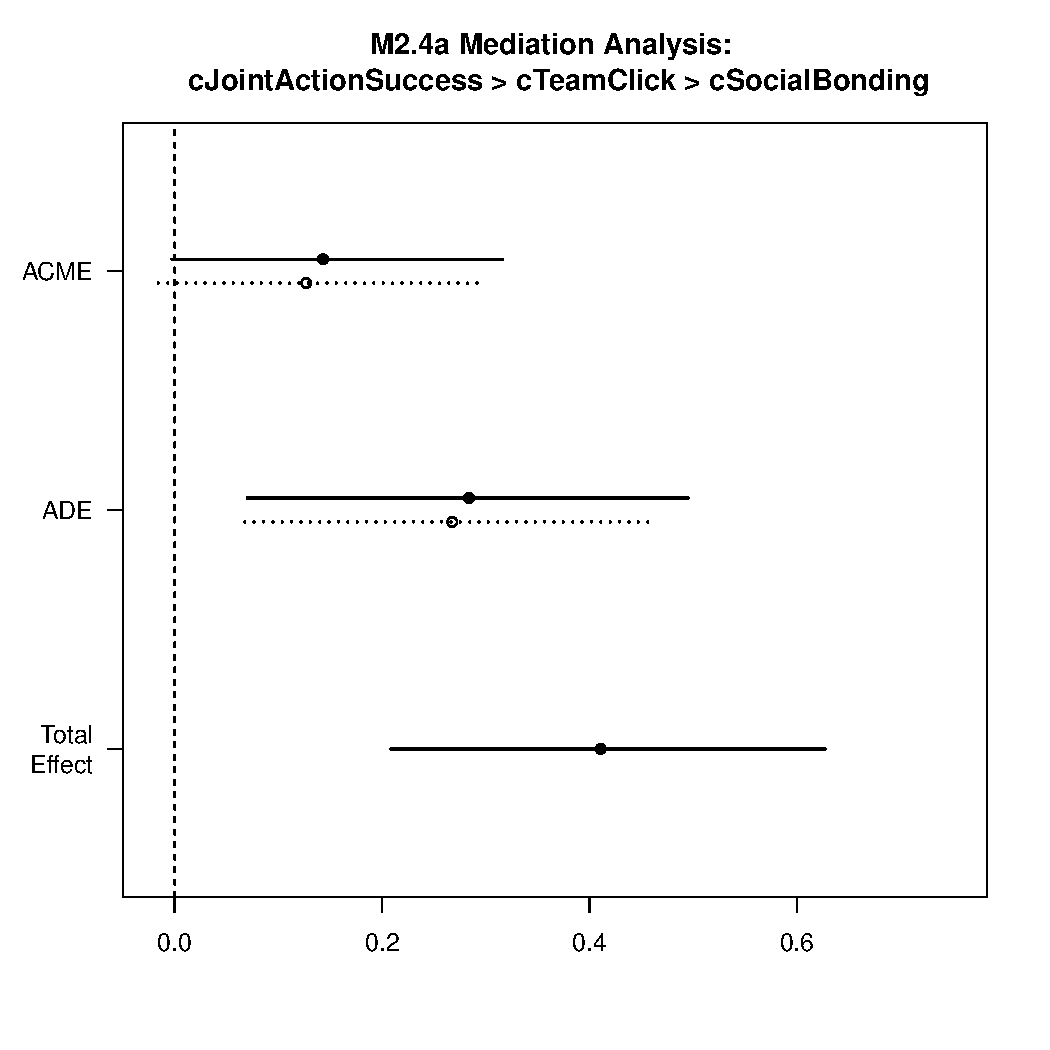
\includegraphics[width=\columnwidth]{images/MLM24aMediationAnalysis.pdf}
  \caption{M24a Mediation Analysis}
  \label{fig:MLM24aMediationAnalysis}
\end{figure}



\subsubsection{Additional Analysis: What predicts change in fusion to family?}
Both verbal and pictorial measures of fusion to team did not vary significantly in pre-post Tournament measures (see descriptives Table ~\ref{tab:factorsPrePostSummary}).  Interestingly, the pictorial measure of fusion to family did increase significantly between pre- and post-Tournament measurements.  Exploratory analysis was performed to investigate the possible correlates of this increase. In line with the predictions of this study, we tested whether 1) changes in perceptions of Joint Action Success, 2) Team Click, and 3) their interaction (Joint Action Success x Team Click) predicted change in fusion to family.

\myparagraph{$\Delta$Fusion Family $\sim$ $\Delta$Joint Action Success}
The first model revealed a significant effect of change in perceptions of joint-action success and change in fusion to family, $\beta = .43$ ($95\% CI =  .07, .79$), $SE = .18$, $t(6.96) = 2.34$, $p = .$, $marginal R^2 = .11$, $conditional R^2 = .14$.  The distribution of residuals indicated a poor model fit, ($W = 0.90$, $p < .00001$), due to high kurtosis ($> 2$), but not skew (.30). Given that log-transformation was not appropriate for normalising kurtosis \citep{Glass1972}, the analysis was re-run after excluding influential outliers.  The adjusted model was a much better fit, with model residuals normally distributed around zero, ($W = 0.99$, $p-value < .60$), see Table ~\ref{tab:MLM25acFusioncJointAction}. The model confirmed a significant positive relationship between change in perceptions of joint-action success and change in fusion to family, $\beta = .36$ ($95\% CI =  .19, .52$), $SE = .08$, $t() = 4.36$, $p = .$, $marginal R^2 = .32$, $conditional R^2 = .32$.


% Table created by stargazer v.5.2 by Marek Hlavac, Harvard University. E-mail: hlavac at fas.harvard.edu
% Date and time: Tue, Jun 27, 2017 - 10:42:15
\begin{table}[!htbp] \centering 
  \caption{cFusionFamily ~ jointActionSuccess} 
  \label{tab:MLM25acFusioncJointAction} 
\footnotesize 
\begin{tabular}{@{\extracolsep{5pt}}lcc} 
\\[-1.8ex]\hline 
\hline \\[-1.8ex] 
 & \multicolumn{2}{c}{\textit{Dependent variable:}} \\ 
\cline{2-3} 
\\[-1.8ex] & cFusionFamily & fusionPictorialFamilyChangeOut \\ 
 &  & outliers removed \\ 
\\[-1.8ex] & (1) & (2)\\ 
\hline \\[-1.8ex] 
 (constant) & 0.12 & $-$0.04 \\ 
  & (0.66) & (0.32) \\ 
  & & \\ 
 cJointActionSuccess & 0.43$^{**}$ & 0.50$^{***}$ \\ 
  & (0.18) & (0.10) \\ 
  & & \\ 
 cIndPerformanceSuccess & $-$0.46$^{**}$ & $-$0.01 \\ 
  & (0.20) & (0.10) \\ 
  & & \\ 
 teamPerformanceExpectations & $-$0.01 & 0.002 \\ 
  & (0.01) & (0.004) \\ 
  & & \\ 
 indPerformanceExpectations & 0.001 & $-$0.003 \\ 
  & (0.01) & (0.004) \\ 
  & & \\ 
 objectiveCompetence & 0.27 & 0.06 \\ 
  & (0.19) & (0.09) \\ 
  & & \\ 
 subjectiveCompetence & 0.06 & $-$0.0003 \\ 
  & (0.16) & (0.08) \\ 
  & & \\ 
 finalRank & 0.10 & $-$0.02 \\ 
  & (0.08) & (0.04) \\ 
  & & \\ 
 minutesTotal & $-$0.002 & 0.01 \\ 
  & (0.01) & (0.004) \\ 
  & & \\ 
\hline \\[-1.8ex] 
Marginal R-squared & .11 & .32 \\ 
Conditional R-squared & .14 & .32 \\ 
Observations & 97 & 97 \\ 
Log Likelihood & $-$173.00 & $-$104.99 \\ 
Akaike Inf. Crit. & 372.00 & 235.98 \\ 
Bayesian Inf. Crit. & 405.48 & 269.45 \\ 
\hline 
\hline \\[-1.8ex] 
\textit{Note:}  & \multicolumn{2}{r}{$^{*}$p$<$0.1; $^{**}$p$<$0.05; $^{***}$p$<$0.01} \\ 
\end{tabular} 
\end{table} 

% Table created by stargazer v.5.2 by Marek Hlavac, Harvard University. E-mail: hlavac at fas.harvard.edu
% Date and time: Tue, Jun 27, 2017 - 10:42:15
\begin{table}[!htbp] \centering 
  \caption{cFusionFamily ~ jointActionSuccess} 
  \label{tab:MLM25acFusioncJointAction} 
\footnotesize 
\begin{tabular}{@{\extracolsep{5pt}} ccc} 
\\[-1.8ex]\hline 
\hline \\[-1.8ex] 
$0.05$ & $0.01$ & $0.001$ \\ 
\hline \\[-1.8ex] 
\end{tabular} 
\end{table} 


%Need to do a multivariate regression here with family, country, team as outcomes?
\myparagraph{$\Delta$fusionFamily $\sim$ $\Delta$Team Click}

This model revealed that change in feelings of team-click was not a significant predictor of change in fusion to family, $\beta = .07$ ($95\% CI =  -.30, .44$), $SE = .19$, $t() = .38$, $p = .$, $marginal R^2 = .04$, $conditional R^2 = .07$. No other predictors in the model were statistically significant.

\myparagraph{$\Delta$fusionFamily $\sim$  $\Delta$Joint Action Success $\times$ $\Delta$Team Click}

The final model included an interaction between change in perceptions of joint-action success and change in feelings of team click as possible predictor of change in fusion to family.  Results of the model revealed that the interaction between change in perceptions of joint-action success and change in feelings of team-click was a significant positive predictor of change in fusion to family, $\beta = .22$ ($95\% CI =  .02, .41$), $SE = .10$, $t() = 2.22$, $p = .$, $marginal R^2 = .17$, $conditional R^2 = .23$. Model residuals were non-normally distributed, ($W = 0.93$, $p < .00001$).\\

This result is consistent with ethnographic findings, whereby the family unit is elevated above the team and other priorities.  This results will be considered in more depth once ethnographic analysis has also been completed.



\subsection{Discussion of Results: pre- to post-Tournament Analysis}
  The results of the pre-post Tournament analysis, like the post-Tournament analysis reported above, provide support for the predictions of this study.  Increases in positive perceptions of joint-action success correlated with a larger increase in feelings of team click pre-post Tournament: athletes who experienced a positive increase in perceptions of joint-action success also reported a positive increase in feelings of team click.  Likewise, those who experienced more positive violations of team performance expectations (measured following the Tournament) also experienced a higher increase in feelings of team click pre-post Tournament.  The interaction between Joint Action Success and Team Performance Expectations, however, was not significant. Further, increases in perception of joint action success (but not team performance expectations) significantly predicted increases in feelings of social bonding before and after the Tournament.  Mediation analysis revealed that variation in team click partially mediated a direct relationship between joint action success and social bonding, however this result was only a significant trend (p = .06).  Team Performance Expectations failed to satisfactorily predict social bonding, and so was not considered in a mediation analysis.












\subsection{Analysis \& results of overall Tournament data}

In the final section of analysis, evidence for a relationship between joint-action success, team click, and social bonding was assessed across the entire data set. Given that the mid-Tournament survey was truncated to accord with athlete schedules and convenience following games, variables that could be analysed across the entire tournament were limited to those that appeared in the mid-Tournament surveys. Time constraints meant that component performance was not assessed in the mid-Tournament survey, and only appraisals of overall individual and team performance relative to prior expectations were included. The mid-Tournament survey contained three team click items (Unspoken Understanding, General Atmosphere, and Click Pictorial), three social bonding items (Emotional Support, Shared Goal, and Fusion Pictorial), and three fatigue items (Fatigue, Physical Exertion, Mental Exertion). These groups of variables were all subjected to data reduction (EFA) for the purposes of analysis.



\subsubsection{Roadmap of Overall Tournament Analysis}
Analysis of the overall Tournament data proceeded in the same step-wise fashion as analyses above. First, the relationship between Team Performance Expectations and team click Team Click was tested, controlling for Tournament performance, perceptions of individual performance, and competence.

\begin{description}
  \item [Prediction 3.1.b] Team Performance Expectations $\rightarrow$ Team Click
\end{description}

Next, the relationship between Team Click and Social Bonding was tested, followed by a test of the direct relationship between Team Performance Expectations and Social Bonding:

\begin{description}
  \item [Prediction 3.2.a] Team Click $\rightarrow$ Social Bonding
  \item [Prediction 3.2.b] Team Performance Expectations $\rightarrow$ Social Bonding
\end{description}
\bigskip
Finally, a mediation analysis was conducted, in which the interaction effect of Team Performance Expectations and team click on social bonding was tested.
\bigskip
\begin{description}
\item[Prediction 3.4.a] Team Performance Expectations^*Team Click  $\rightarrow$ Social Bonding
\item[Prediction 3.4.b] Mediation Analysis: Team Performance Expectations $\rightarrow$ Team Click $\rightarrow$ Social Bonding
\end{description}
\clearpage




\subsubsection{Overall Tournament Descriptive Analysis}

Tables~\ref{tab:performanceOverallSummary}\nobreakdash--\ref{tab:fatigueOverallSummary} display basic summary statistics (mean and standard deviation) for variables of interest at each recorded time point. Almost all variables of interest under the categories of performance, team click, social bonding and fatigue have means above the mid-point of each scale. In addition, mid-Tournament measurements tend to be lower than pre- or post-Tournament measures for each category. In relation to performance measures, for example, athletes appear on average to be more critical of their own and their team’s performance (relative to prior expectations) when surveyed immediately after games on day 1 and 2 than they were following the Tournament (note, however, that survey items relating to individual and team performance administered pre-Tournament were not posed in relation to athlete expectations, and thus could not be directly compared to subsequent mid- and post-Tournament measures). The same pattern was identifiable in team click variables, with the means for mid-Tournament measures of Unspoken Understanding and General Atmosphere 10-15\% lower than pre- or post-Tournament measures. This is also the case for variables related to social bonding: Emotional Support and Shared Goal in particular showing a steep increase form mid-Tournament measurements to the post-Tournament measurement. The same pattern was identifiable for variables relevant to fatigue (see Table ~\ref{tab:fatigueOverallSummary}).


% Table created by stargazer v.5.2 by Marek Hlavac, Harvard University. E-mail: hlavac at fas.harvard.edu
% Date and time: Mon, Jun 26, 2017 - 09:48:21
\begin{table}[!htbp] \centering 
  \caption{Overall Tournament Performance Summary Statistics} 
  \label{tab:performanceOverallSummary} 
\scriptsize 
\begin{tabular}{@{\extracolsep{5pt}} ccccccccc} 
\\[-1.8ex]\hline 
\hline \\[-1.8ex] 
time & teamPerf & tP.sd & indPerf & iP.sd & teamPerfExp & tPE.sd & indPerfExp & iP.sd.1 \\ 
\hline \\[-1.8ex] 
pre-Tournament & $71.11$ & $21.87$ & $68.92$ & $21.32$ & $$ & $$ & $$ & $$ \\ 
day1 & $$ & $$ & $$ & $$ & $54.43$ & $30.63$ & $39.43$ & $27.25$ \\ 
day2 & $$ & $$ & $$ & $$ & $53.19$ & $32.98$ & $40.92$ & $27.93$ \\ 
post-Tournament & $$ & $$ & $$ & $$ & $64.36$ & $23.61$ & $56.36$ & $23.47$ \\ 
\hline \\[-1.8ex] 
\end{tabular} 
\end{table} 


% Table created by stargazer v.5.2 by Marek Hlavac, Harvard University. E-mail: hlavac at fas.harvard.edu
% Date and time: Mon, Jun 26, 2017 - 09:21:29
\begin{table}[!htbp] \centering 
  \caption{Team Click Overall Tournament Summary Statistics} 
  \label{tab:clickOverallSummary} 
\scriptsize 
\begin{tabular}{@{\extracolsep{5pt}} ccccccc} 
\\[-1.8ex]\hline 
\hline \\[-1.8ex] 
time & unspUnd & uU.sd & genAt & gA.sd & clickPic & cP.sd \\ 
\hline \\[-1.8ex] 
pre-Tournament & $71.58$ & $20.77$ & $75.51$ & $23.27$ & $3.87$ & $1.24$ \\ 
day1 & $55.92$ & $26.88$ & $65.74$ & $31.95$ & $3.46$ & $1.49$ \\ 
day2 & $55.30$ & $29.43$ & $64.32$ & $33.39$ & $3.33$ & $1.70$ \\ 
post-Tournament & $72.72$ & $19.95$ & $78.45$ & $21.34$ & $3.93$ & $1.04$ \\ 
\hline \\[-1.8ex] 
\end{tabular} 
\end{table} 


% Table created by stargazer v.5.2 by Marek Hlavac, Harvard University. E-mail: hlavac at fas.harvard.edu
% Date and time: Mon, Jun 26, 2017 - 09:22:14
\begin{table}[!htbp] \centering 
  \caption{Social Bonding Overall Tournament Summary Statistics} 
  \label{tab:bondingOverallSummary} 
\scriptsize 
\begin{tabular}{@{\extracolsep{5pt}} ccccccc} 
\\[-1.8ex]\hline 
\hline \\[-1.8ex] 
time & emoSup & eS.sd & sharedGoal & sG.sd & fusionPic & fP.sd \\ 
\hline \\[-1.8ex] 
pre-Tournament & $70.12$ & $26.21$ & $77.66$ & $24.28$ & $4.26$ & $1.25$ \\ 
day1 & $67.29$ & $30.56$ & $76.34$ & $30.50$ & $4.06$ & $1.47$ \\ 
day2 & $67.53$ & $32.55$ & $71.42$ & $35.47$ & $3.85$ & $1.69$ \\ 
post-Tournament & $79.67$ & $18.84$ & $86$ & $15.56$ & $4.33$ & $1.19$ \\ 
\hline \\[-1.8ex] 
\end{tabular} 
\end{table} 


% Table created by stargazer v.5.2 by Marek Hlavac, Harvard University. E-mail: hlavac at fas.harvard.edu
% Date and time: Mon, Jun 26, 2017 - 09:23:43
\begin{table}[!htbp] \centering 
  \caption{Fatigue Overall Tournament Summary Statistics} 
  \label{tab:fatigueOverallSummary} 
\scriptsize 
\begin{tabular}{@{\extracolsep{5pt}} ccccccccc} 
\\[-1.8ex]\hline 
\hline \\[-1.8ex] 
time & fat & f.sd & prpe & p.sd & mental & m.sd & inj.mu & inj.sd \\ 
\hline \\[-1.8ex] 
pre-Tournament & $$ & $$ & $$ & $$ & $$ & $$ & $18.73$ & $23.36$ \\ 
day1 & $50.14$ & $28.80$ & $12.45$ & $4.52$ & $4.09$ & $2.83$ & $29.91$ & $33.15$ \\ 
day2 & $53.65$ & $31.03$ & $12.60$ & $5.53$ & $4.13$ & $3.17$ & $37.14$ & $37.66$ \\ 
post-Tournament & $69.27$ & $21.24$ & $14.97$ & $2.66$ & $6.08$ & $2.47$ & $23.86$ & $26.91$ \\ 
\hline \\[-1.8ex] 
\end{tabular} 
\end{table} 


%<<surveyMeasureSummaryTable, fig.cap =''>>=
%#create all columns:
%Items <- c(IndPerformance, GroupPerformance, TeamPerformance, GroupClick, TeamClick, GroupBonding, TeamBonding, Arousal, Exertion)
%Baseline <- c("*","","*","","*","","*","","")
%Pre <- c("*","*","","*","","*","","*","")
%Post <- c("*","*","","*","*","*","*","*","*")

%surveyMeasureSummary <- data.frame(Variable, Baseline, Pre, Post, stringsAsFactors = FALSE)

%summaryTable <- xtable(surveyMeasureSummary)
%align(summaryTable) <- xalign(summaryTable)
%summaryTable
%@



\subsubsection{Data Reduction}

Data reduction was performed in order to consolidate outcome variables and reduce multicolinearity of predictor variables. There were only single items for individual and team performance items, and so EFA was not required. Variables relevant to team click, social bonding, and fatigue and measured at each time point across the entire Tournament  were subjected to an EFA.

For Team Click, Unspoken Understanding, General Atmosphere, and Click Pictorial were subjected to EFA.  Correlations between variables were high, suggesting that imposing one factor was appropriate (all $r's > .62$, $KMO = 0.7$, $\chi^2(3, N = 440) = 723.67$).  The factor ``Team Click Tournament'' explained 70.3\% of the variance (SS Loadings = 2.11).  $Guttman's \lambda =.83$ and Cronbach's $\alpha = .87$ indicated that the data reduction was appropriate.

Three variables related to social bonding (Emotional Support, Shared Goal, and Fusion Pictorial) were subjected to EFA. Correlations between variables were high, suggesting that imposing one factor was appropriate (all $r's > .63$, $KMO = 0.71$, $\chi^2(3, N = 440) =  759.30$, $p < .001$).  The factor imposed for Social Bonding (``Social Bonding Tournament'') explained 71.7\% of the variance ($SS Loadings =  2.15$), and $Guttman's \lambda =.84$ and $Cronbach's \alpha= .88$ indicated that the data reduction was reliable.

Fatigue items consisted of fatigue, physical exertion and mental exertion. Correlations between variables were high, indicating that imposing one factor was appropriate (all $r's > .62$, $KMO = 0.71$, $\chi^2(3, N = 440) =  677.37, p < .001$).  The factor imposed for fatigue, ``Fatigue Tournament,'' explained 69\% of the variance ($SS Loading = 2.07$) and $Guttman's \lambda =.82$ and Cronbach's $\alpha = .87$) indicated that the data reduction was reliable.

All other variables used in the Overall Tournament analysis were single item variables and did not require data reduction.





\subsection{Overall Tournament Results}
In the final section, the entire data set was utilised to analyse a relationship between joint-action, team click, and social bonding. As described in the previous section, items relating to performance, team click, and social bonding that were consistent across the data set were reduced to factors in order to test study predictions. The repeated measures design of this analysis made it possible to statistically account for variation in responses due to repeated sampling of the same individual athlete throughout the Tournament, and due to the fact that each athlete was member of a specific team. The following models used a three-level structure, with responses across the four time points (level 1) nested within individual athletes (level 2), who were nested within individual teams (level 3). Both the slopes and intercepts were allowed to vary for every fixed effect of the model.


\subsubsection{3.1.b Team Click $\sim$ Team Performance Expectations}

 The first model tested the predicted relationship between joint-action and team click:
   \begin{equation}

\end{equation}    \begin{align*}
       Team Click =  & Team Performance Expectations  \\
                 &+ Individual Performance Expectations   \\
                 &+ Objective Competence + Subjective Competence \\
                 &+ TournamentPerformanceMeasures  \\
     \end{align*}
   \end{equation}
   \bigskip

 The model revealed a significant relationship between team performance expectation violation and team click, $\beta = .71$ ($95\% CI =  .0.62, .80$), $SE = .001$, $t(193.20) = 16.29$, $p < .0001$, $marginal R^2 = .63$, $conditional R^2 = .69$.
 The model also indicated that individual performance expectation violation significantly predicted team click, $\beta = .004$ ($95\% CI =  .04, .20$), $SE = .04$, $t(311.7) = 2.81$, $p < .01$, as did Subjective Competence, $\beta = .08$ ($95\% CI =  .002, .15$), $SE = .04$, $t(292) = 2.00$, $p = .02$  (see Table ~\ref{tab:MLM31ateamPerfClickTournament} for full description of results).
 The residuals of the model were normally distributed around zero, ($W = 0.99, p = .11$), and individual cases had low influence on the model (Cook's Distances all < .05) (see Appendix Figure ~\ref{fig:MLM31aTeamPerfExpClick}).
 Results of the model suggest that, when controlling for individual performance, measures of objective and subjective competence, and Tournament performance, athletes whose expectations around team performance were more positively violated also experienced stronger feelings of team click. Overall, it also appears that more positive expectations about individual performance, and higher levels of self-reported technical competence predicted higher levels of team click.



 
\begin{table}
\begin{center}
\begin{tabular}{l c c c }
\toprule
 & Intercept & Main effect & Controls \\
\midrule
(constant)                                                        & $-0.00$  & $-0.06$               & $-0.12$               \\
                                                                  & $(0.04)$ & $(0.03)$              & $(0.21)$              \\
Team Performance Vs Expectations                                  &          & $\mathbf{0.74}^{***}$ & $\mathbf{0.72}^{***}$ \\
                                                                  &          & $(0.03)$              & $(0.05)$              \\
Ind Performance Vs Expectations                                   &          &                       & $\mathbf{0.12}^{**}$  \\
                                                                  &          &                       & $(0.04)$              \\
Objective Competence                                              &          &                       & $0.04$                \\
                                                                  &          &                       & $(0.04)$              \\
Subjective Competence                                             &          &                       & $0.07$                \\
                                                                  &          &                       & $(0.04)$              \\
Final Rank                                                        &          &                       & $-0.00$               \\
                                                                  &          &                       & $(0.02)$              \\
Minutes Total                                                     &          &                       & $-0.00$               \\
                                                                  &          &                       & $(0.00)$              \\
Points Total                                                      &          &                       & $0.00$                \\
                                                                  &          &                       & $(0.00)$              \\
Fatigue                                                           &          &                       & $0.00$                \\
                                                                  &          &                       & $(0.00)$              \\
Extraverted                                                       &          &                       & $0.01$                \\
                                                                  &          &                       & $(0.03)$              \\
\midrule
AIC                                                               & 1552.70  & 842.67                & 602.59                \\
BIC                                                               & 1570.04  & 879.53                & 665.89                \\
Log Likelihood                                                    & -772.35  & -412.33               & -284.30               \\
Num. obs.                                                         & 564      & 444                   & 306                   \\
\bottomrule
\multicolumn{4}{l}{\scriptsize{Coefficients with $p < 0.05$ in \textbf{bold}. Marginal $R^2 = .63$, Conditional $R^2 = .69$}}
\end{tabular}
\caption{Prediction 1: Team Performance Vs Expectations predicts Team Click in the Overall Tournament survey data (n = 90).}
\label{tab:MLM31ateamPerfClickTournament}
\end{center}
\end{table}




\subsubsection{3.2.a Social Bonding $\sim$ Team Click}
 The relationship between team click and social bonding was tested. Controlling for perceptions of individual performance, measures of objective and subjective competence, and Tournament performance, the model revealed a significant positive relationship between feelings of team click and feelings of social bonding, $\beta = .64$ ($95\% CI = .56, .74$), $SE = .05$, $t(87.4) = 13.84$, $p < .0001$, $marginal R^2 = .49$, $conditional R^2 = .66$ (see Table ~\ref{tab:MLM31bclickBondingTournament} for complete description of model estimates). Model residuals were not normally distributed around zero, ($W = 0.92, p < .00001$), owing to high negative skew ($-1.24$) and high kurtosis (5.12) (see Appendix Figure ~\ref{fig:MLM31bAssumptions}).
 Both log transformation ($W = 0.95, p < .00001$) and outlier removal ($W = 0.96, p < .00001$) procedures improved the model fit marginally, but not within the bounds of normality.
 To resolve this assumption violation, the outcome variable was first subjected to outlier-removal, and then subsequently log-transformed, which appeared to improve the distribution of residuals somewhat, ($W = 0.98, p = .0002$, see Table ~\ref{MLM31bclickBondingTournamentModelComparison} for adjusted model comparisons and Appendix Figure ~\ref{fig:MLM31bLogOutAssumptions} for adjusted model residuals).
 The adjusted model failed to converge, and so a

 confirmed a significant positive effect of team click on social bonding over the course of the Tournament, $\beta = .19$ ($95\% CI =  .15, .23$), $SE = .05$, $t() = 9.89$, $p < .001$, $marginal R^2 = .30$, $conditional R^2 = .43$.  These results suggest that on average, athletes who experienced higher feelings of team click also experienced higher levels of social bonding throughout the course of the Tournament.

 
% Table created by stargazer v.5.2 by Marek Hlavac, Harvard University. E-mail: hlavac at fas.harvard.edu
% Date and time: Thu, Sep 14, 2017 - 09:39:55
\begin{table}[!htbp] \centering 
  \caption{bondingTournament ~ teamClickTournament} 
  \label{tab:MLM31bclickBondingTournament} 
\footnotesize 
\begin{tabular}{@{\extracolsep{5pt}}lccc} 
\\[-1.8ex]\hline 
\hline \\[-1.8ex] 
 & \multicolumn{3}{c}{\textit{Dependent variable:}} \\ 
\cline{2-4} 
\\[-1.8ex] & (1) & (2) & (3)\\ 
\hline \\[-1.8ex] 
 (constant) & $-$0.00 & $-$1.46$^{***}$ & $-$1.59$^{***}$ \\ 
  & (0.04) & (0.08) & (0.15) \\ 
  & & & \\ 
 teamPerformanceExpectations &  & 0.02$^{***}$ & 0.02$^{***}$ \\ 
  &  & (0.001) & (0.001) \\ 
  & & & \\ 
 indPerformanceExpectations &  &  & 0.004$^{**}$ \\ 
  &  &  & (0.002) \\ 
  & & & \\ 
 objectiveCompetence &  &  & 0.02 \\ 
  &  &  & (0.04) \\ 
  & & & \\ 
 subjectiveCompetence &  &  & 0.08$^{*}$ \\ 
  &  &  & (0.04) \\ 
  & & & \\ 
 finalRank &  &  & $-$0.0002 \\ 
  &  &  & (0.02) \\ 
  & & & \\ 
 minutesTotal &  &  & $-$0.001 \\ 
  &  &  & (0.002) \\ 
  & & & \\ 
 pointsTotal &  &  & 0.003 \\ 
  &  &  & (0.003) \\ 
  & & & \\ 
\hline \\[-1.8ex] 
Marginal R-squared & .47 & .49 &  \\ 
Conditional R-squared & .66 & .66 &  \\ 
Observations & 564 & 444 & 331 \\ 
Log Likelihood & $-$772.35 & $-$412.33 & $-$303.82 \\ 
Akaike Inf. Crit. & 1,552.70 & 842.67 & 637.65 \\ 
Bayesian Inf. Crit. & 1,570.04 & 879.53 & 694.68 \\ 
\hline 
\hline \\[-1.8ex] 
\textit{Note:}  & \multicolumn{3}{r}{$^{*}$p$<$0.05; $^{**}$p$<$0.01; $^{***}$p$<$0.001} \\ 
\end{tabular} 
\end{table} 


 
% Table created by stargazer v.5.2 by Marek Hlavac, Harvard University. E-mail: hlavac at fas.harvard.edu
% Date and time: Thu, Sep 14, 2017 - 09:39:58
\begin{table}[!htbp] \centering 
  \caption{Model Adjustment Comparison:bondingTournament ~ teamClickTournament} 
  \label{MLM31bclickBondingTournamentModelComparison} 
\tiny 
\begin{tabular}{@{\extracolsep{5pt}}lcccc} 
\\[-1.8ex]\hline 
\hline \\[-1.8ex] 
 & \multicolumn{4}{c}{\textit{Dependent variable:}} \\ 
\cline{2-5} 
 & model & log-transformed & outliers removed & outliers + log-transformed \\ 
\\[-1.8ex] & (1) & (2) & (3) & (4)\\ 
\hline \\[-1.8ex] 
 (constant) & $-$1.59$^{***}$ & 1.63$^{***}$ & 0.31$^{***}$ & 1.50$^{***}$ \\ 
  & (0.15) & (0.02) & (0.08) & (0.04) \\ 
  & & & & \\ 
 teamPerformanceExpectations & 0.02$^{***}$ &  &  &  \\ 
  & (0.001) &  &  &  \\ 
  & & & & \\ 
 indPerformanceExpectations & 0.004$^{**}$ &  &  &  \\ 
  & (0.002) &  &  &  \\ 
  & & & & \\ 
 objectiveCompetence &  & 0.16$^{***}$ & 0.42$^{***}$ & 0.19$^{***}$ \\ 
  &  & (0.01) & (0.04) & (0.02) \\ 
  & & & & \\ 
 subjectiveCompetence & 0.02 & 0.01 & 0.01 & 0.01 \\ 
  & (0.04) & (0.01) & (0.03) & (0.01) \\ 
  & & & & \\ 
 finalRank & 0.08$^{*}$ & 0.01 & 0.03 & 0.02 \\ 
  & (0.04) & (0.01) & (0.02) & (0.01) \\ 
  & & & & \\ 
 minutesTotal & $-$0.0002 & $-$0.004 & $-$0.01 & $-$0.01 \\ 
  & (0.02) & (0.003) & (0.01) & (0.005) \\ 
  & & & & \\ 
 pointsTotal & $-$0.001 & $-$0.001 & $-$0.002 & $-$0.001 \\ 
  & (0.002) & (0.0004) & (0.001) & (0.001) \\ 
  & & & & \\ 
 pointsTotal & 0.003 & $-$0.001 & $-$0.001 & $-$0.001 \\ 
  & (0.003) & (0.001) & (0.002) & (0.001) \\ 
  & & & & \\ 
\hline \\[-1.8ex] 
Marginal R-squared & .49 & .50 & .23 & .23 \\ 
Conditional R-squared & .66 & .61 & .35 & .34 \\ 
Shapiro-Wilk Test (p-value) & .92(<.00000000001) & .95(<.000001) & .96(<.00001) & .98(.0002) \\ 
Observations & 331 & 449 & 405 & 405 \\ 
Log Likelihood & $-$303.82 & 225.59 & $-$241.97 & 79.71 \\ 
Akaike Inf. Crit. & 637.65 & $-$423.18 & 511.94 & $-$131.42 \\ 
Bayesian Inf. Crit. & 694.68 & $-$365.69 & 567.99 & $-$75.37 \\ 
\hline 
\hline \\[-1.8ex] 
\textit{Note:}  & \multicolumn{4}{r}{$^{*}$p$<$0.05; $^{**}$p$<$0.01; $^{***}$p$<$0.001} \\ 
\end{tabular} 
\end{table} 



\subsubsection{3.2.b Social Bonding $\sim$ Team Performance Expectations}
The direct relationship between Team Performance Expectations and social bonding was tested.  The initial model failed to converge with the random slope and intercept model structure.  As such, the model was simplified to estimate only the random slope. This simplified model revealed a significant positive relationship between team performance expectation violation and social bonding, $\beta = .46$ ($95\% CI =  .35, .57$), $SE = .05$, $t(331.00) = 8.48$, $p < .0001$, $marginal R^2 = .40$, $conditional R^2 = .40$.
The model also revealed a significant relationship between Individual Performance Expectations and social bonding, $\beta = .005$ ($95\% CI =  .002, .009$), $SE = .002$, $t(303.4) = 2.80$, $p < .01$, as well as subjective competence and social bonding, $\beta = .01$ ($95\% CI =  .01, .18$), $SE = .04$, $t(265.3) = 2.24$, $p = .03$ (see Table ~\ref{tab:MLM32ateamPerfBondingTournament} for full description of model estimates).

Model residuals were non-normally distributed, ($W = 0.97, p < .00001$), with negative skew ($-.6$), and higher than normal kurtosis, see Appendix Figure ~\ref{fig:MLM32aAssumptions}.  A model in which the outcome was log-transformed following removal of outliers provided the best possible fit for the available data ~\ref{MLM32ateamPerfBondingTournamentModelComparison}. While the distribution of errors was still non-normal, ($W = 0.99, p = .03$),  error terms appear much more evenly distributed around zero than the original model, albeit with a slight negative skew ($-0.1$).
The adjusted model confirmed the significant positive effect of team performance expectation violation on social bonding,  $\beta = .16$ ($95\% CI =  .12, .20$), $SE = .02$, $t(336.80) = 7.98$, $p < .0001$, $marginal R^2 = .36$, $conditional R^2 = .36$.



 
\begin{table}
\begin{center}
\begin{tabular}{l c c c c }
\toprule
 & Main effect & Controls & Log-transformed & Log and outliers \\
\midrule
(constant)                        & $-0.00$               & $\mathbf{0.51}^{*}$   & $\mathbf{1.71}^{***}$ & $\mathbf{1.64}^{***}$ \\
                                  & $(0.04)$              & $(0.26)$              & $(0.06)$              & $(0.08)$              \\
Team Performance Vs Expectations  & $\mathbf{0.59}^{***}$ & $\mathbf{0.47}^{***}$ & $\mathbf{0.11}^{***}$ & $\mathbf{0.07}^{***}$ \\
                                  & $(0.04)$              & $(0.06)$              & $(0.01)$              & $(0.02)$              \\
Ind Performance Vs Expectations   &                       & $\mathbf{0.25}^{***}$ & $\mathbf{0.05}^{***}$ & $0.01$                \\
                                  &                       & $(0.06)$              & $(0.01)$              & $(0.02)$              \\
Objective Competence              &                       & $0.07$                & $0.02$                & $0.01$                \\
                                  &                       & $(0.05)$              & $(0.01)$              & $(0.02)$              \\
Subjective Competence             &                       & $0.09$                & $\mathbf{0.02}^{*}$   & $\mathbf{0.03}^{*}$   \\
                                  &                       & $(0.05)$              & $(0.01)$              & $(0.01)$              \\
Final Rank                        &                       & $-0.03$               & $-0.01$               & $-0.01$               \\
                                  &                       & $(0.02)$              & $(0.01)$              & $(0.01)$              \\
Minutes Total                   &                       & $-0.01$  & $-0.00$  & $-0.00$               \\
                                  &                       & $(0.00)$              & $(0.00)$              & $(0.00)$              \\
Points Total                      &                       & $0.00$                & $0.00$                & $0.00$                \\
                                  &                       & $(0.00)$              & $(0.00)$              & $(0.00)$              \\
Fatigue                           &                       & $0.00$                & $0.00$                & $0.00$                \\
                                  &                       & $(0.00)$              & $(0.00)$              & $(0.00)$              \\
Extraverted                       &                       & $-0.04$               & $-0.01$               & $-0.02$               \\
                                  &                       & $(0.03)$              & $(0.01)$              & $(0.01)$              \\
\midrule
AIC                               & 1083.79               & 752.42                & -131.94               & -8.28                 \\
BIC                               & 1104.27               & 800.83                & -83.53                & 38.54                 \\
Log Likelihood                    & -536.89               & -363.21               & 78.97                 & 17.14                 \\
Num. obs.                         & 444                   & 306                   & 306                   & 271                   \\
\bottomrule
\multicolumn{5}{l}{\scriptsize{Coefficients with $p < 0.05$ in \textbf{bold}. Effect sizes of the Log and outlier model: Marginal $R^2 = .36$, Conditional $R^2 = .36$}}
\end{tabular}
\caption{Prediction 3: Team Performance Vs Expectations predicts Social Bonding in the Overall Tournament survey data (n = 90).}
\label{tab:MLM32ateamPerfBondingTournament}
\end{center}
\end{table}


 
% Table created by stargazer v.5.2 by Marek Hlavac, Harvard University. E-mail: hlavac at fas.harvard.edu
% Date and time: Thu, Sep 14, 2017 - 09:42:11
\begin{table}[!htbp] \centering 
  \caption{Model Comparison: M3.2a socialBondingTournament ~ teamPerformanceExpectationsTournament} 
  \label{tab:MLM32ateamPerfBondingTournamentModelComparison} 
\scriptsize 
\begin{tabular}{@{\extracolsep{5pt}}lccc} 
\\[-1.8ex]\hline 
\hline \\[-1.8ex] 
 & \multicolumn{3}{c}{\textit{Dependent variable:}} \\ 
\cline{2-4} 
 & model & log-transformed & outliers+log-transformed \\ 
\\[-1.8ex] & (1) & (2) & (3)\\ 
\hline \\[-1.8ex] 
 (constant) & $-$0.70$^{***}$ & 1.42$^{***}$ & 1.42$^{***}$ \\ 
  & (0.18) & (0.04) & (0.06) \\ 
  & & & \\ 
 teamPerformanceExpectations & 0.01$^{***}$ & 0.003$^{***}$ & 0.003$^{***}$ \\ 
  & (0.002) & (0.0005) & (0.001) \\ 
  & & & \\ 
 indPerformanceExpectations & 0.01$^{**}$ & 0.001$^{**}$ & 0.0001 \\ 
  & (0.002) & (0.0004) & (0.001) \\ 
  & & & \\ 
 objectiveCompetence & 0.04 & 0.01 & 0.01 \\ 
  & (0.05) & (0.01) & (0.02) \\ 
  & & & \\ 
 subjectiveCompetence & 0.10$^{*}$ & 0.03$^{*}$ & 0.03$^{*}$ \\ 
  & (0.04) & (0.01) & (0.01) \\ 
  & & & \\ 
 finalRank & $-$0.04 & $-$0.01 & $-$0.01 \\ 
  & (0.02) & (0.005) & (0.01) \\ 
  & & & \\ 
 minutesTotal & $-$0.003 & $-$0.001 & $-$0.001 \\ 
  & (0.002) & (0.001) & (0.001) \\ 
  & & & \\ 
 pointsTotal & 0.001 & 0.0001 & 0.0000 \\ 
  & (0.004) & (0.001) & (0.001) \\ 
  & & & \\ 
\hline \\[-1.8ex] 
Marginal R-squared & .33 & .11 & .09 \\ 
Conditional R-squared & .53 & .23 & .17 \\ 
Shapiro-Wilk Test (p-value) & .97($<$.00001) & .96($<$.00001) & .97($<$.00001) \\ 
Observations & 331 & 331 & 294 \\ 
Log Likelihood & $-$373.85 & 96.45 & 21.56 \\ 
Akaike Inf. Crit. & 777.70 & $-$162.91 & $-$13.13 \\ 
Bayesian Inf. Crit. & 834.73 & $-$105.88 & 42.13 \\ 
\hline 
\hline \\[-1.8ex] 
\textit{Note:}  & \multicolumn{3}{r}{$^{*}$p$<$0.05; $^{**}$p$<$0.01; $^{***}$p$<$0.001} \\ 
\end{tabular} 
\end{table} 





\subsubsection{3.4.a Social Bonding $\sim$ Team Performance Expectations Tournament $\times$ Team Click Tournament}

 The interaction of Team Performance Expectations and Team Click was added to the model as a fixed effect to see if an increase in social bonding associated with more positive violations of team performance expectations was heightened when feelings of team-click increased. The model revealed a significant negative interaction between Team Performance Expectations and Team Click,  $\beta = -.26$ ($95\% CI =  -.32, -.20$), $SE = .03$, $t(321.2) = -8.46$, $p < .0001$, $marginal R^2 = .69$, $conditional R^2 = .74$.  Model residuals were non-normal ($W = 0.94, p < .00001$), owing to high kurtosis ($.39$) and negative skew ($-.88$) (see Appendix Figure ~\ref{fig:MLM32aAssumptions}).
 A model in which the outcome variable was log transformed following exclusion of outliers provided the best adjustment: model residuals were normally distributed ($W = 0.99, p = .14$) and individual observations exerted low influence (Cook's Distances all < .10) (see Table ~\ref{MLM33ateamPerfBondingTournamentInteractionComparison} for full model comparison). The adjusted model revealed a significant positive interaction of Team Performance Expectations and Team Click on Social Bonding, $\beta = -.06$ ($95\% CI =  .0004, .002$), $SE = .01$, $t(310.1) = -4.73$, $p < .001$, $marginal R^2 = .61$, $conditional R^2 = .65$.

 These results supported the prediction that feelings of team-click condition the relationship between perceptions of team performance (expectation violation, in this case) and feelings of social bonding.  Below, formal mediation analysis was conducted to further test this relationship.


 
% Table created by stargazer v.5.2 by Marek Hlavac, Harvard University. E-mail: hlavac at fas.harvard.edu
% Date and time: Thu, Sep 14, 2017 - 09:52:55
\begin{table}[!htbp] \centering 
  \caption{M3.3a socialBondingTournament ~ teamPerformanceExpectationsTournament*teamClickTournament} 
  \label{tab:MLM33ateamPerfBondingTournamentInteractionComparison} 
\scriptsize 
\begin{tabular}{@{\extracolsep{5pt}}lccc} 
\\[-1.8ex]\hline 
\hline \\[-1.8ex] 
 & \multicolumn{3}{c}{\textit{Dependent variable:}} \\ 
\cline{2-4} 
 & model & log-transformed & outliers+log-transformed \\ 
\\[-1.8ex] & (1) & (2) & (3)\\ 
\hline \\[-1.8ex] 
 (constant) & 0.45$^{**}$ & 1.69$^{***}$ & 1.62$^{***}$ \\ 
  & (0.16) & (0.04) & (0.06) \\ 
  & & & \\ 
 teamPerformanceExpectations & $-$0.0001 & $-$0.0003 & $-$0.001 \\ 
  & (0.002) & (0.0004) & (0.001) \\ 
  & & & \\ 
 indPerformanceExpectations & 1.02$^{***}$ & 0.22$^{***}$ & 0.11$^{**}$ \\ 
  & (0.06) & (0.01) & (0.04) \\ 
  & & & \\ 
 objectiveCompetence & 0.001 & 0.0003 & $-$0.0001 \\ 
  & (0.001) & (0.0004) & (0.001) \\ 
  & & & \\ 
 subjectiveCompetence & 0.01 & 0.01 & 0.01 \\ 
  & (0.04) & (0.01) & (0.01) \\ 
  & & & \\ 
 finalRank & 0.05 & 0.01 & 0.02 \\ 
  & (0.04) & (0.01) & (0.01) \\ 
  & & & \\ 
 minutesTotal & $-$0.03$^{*}$ & $-$0.01$^{*}$ & $-$0.01 \\ 
  & (0.02) & (0.004) & (0.01) \\ 
  & & & \\ 
 pointsTotal & $-$0.003 & $-$0.001 & $-$0.001 \\ 
  & (0.002) & (0.0005) & (0.001) \\ 
  & & & \\ 
 pointsTotal & 0.001 & 0.0001 & $-$0.001 \\ 
  & (0.003) & (0.001) & (0.001) \\ 
  & & & \\ 
 teamPerformanceExpectations:clickFactor3 & $-$0.01$^{***}$ & $-$0.002$^{***}$ & 0.002$^{*}$ \\ 
  & (0.001) & (0.0003) & (0.001) \\ 
  & & & \\ 
\hline \\[-1.8ex] 
Marginal R-squared & .68 & .28 & .23 \\ 
Conditional R-squared & .73 & .36 & .28 \\ 
Shapiro-Wilk Test (p-value) & .93($<$.00001) & .99(.02) & .99(.14) \\ 
Observations & 331 & 331 & 294 \\ 
Log Likelihood & $-$277.92 & 176.98 & 57.06 \\ 
Akaike Inf. Crit. & 589.83 & $-$319.96 & $-$80.12 \\ 
Bayesian Inf. Crit. & 654.47 & $-$255.32 & $-$17.50 \\ 
\hline 
\hline \\[-1.8ex] 
\textit{Note:}  & \multicolumn{3}{r}{$^{*}$p$<$0.05; $^{**}$p$<$0.01; $^{***}$p$<$0.001} \\ 
\end{tabular} 
\end{table} 








%  plot() interaction





\subsubsection{3.4.b Mediation Analysis: Team Performance Expectations -> Team Click -> Social Bonding}

A mediation analysis was performed to formally test whether feelings of team click over the course of the Tournament mediated a direct relationship between team performance expectation violations and social bonding.  Results outlined above demonstrate Tournament-wide significant positive relationships between team performance expectation violations and feelings of team click, as well as team click and social bonding. Models also demonstrate a direct relationship between expectations around team performance and social bonding.  Available statistical software can only support a 2-level structure for multilevel mediation analysis. The third team-level random effect was therefore dropped from the model, while the model controlled for the random effect of individual across each of the four time points.

Results of the mediation analysis revealed that the average indirect effect of change in Joint Action Success on change in Social Bonding attributable to change in Team Click was highly significant albeit small, $\beta = .02, 95\% CI = .018 , .026, p < .001$.  When controlling for the effect of team click on social bonding, the average direct effect of Team Performance Expectations and Social Bonding was also significant, $\beta = .01, 95\% CI = .001 , .017, p < .00001$.  The total effect of the meditation was also significant, $\beta = .03, 95\% CI = .027, .041, p < .0001$ (see Appendix Figure ~\ref{fig:MLM34aMediationAnalysis}).
These results suggest that Team Click \textit{partially} mediates the effect of Team Performance Expectations and Social Bonding (average proportion mediated = .66 (.57, .77)).  This result should be treated with additional caution, as it did not account for team-level variation.


\begin{figure}[htbp]
  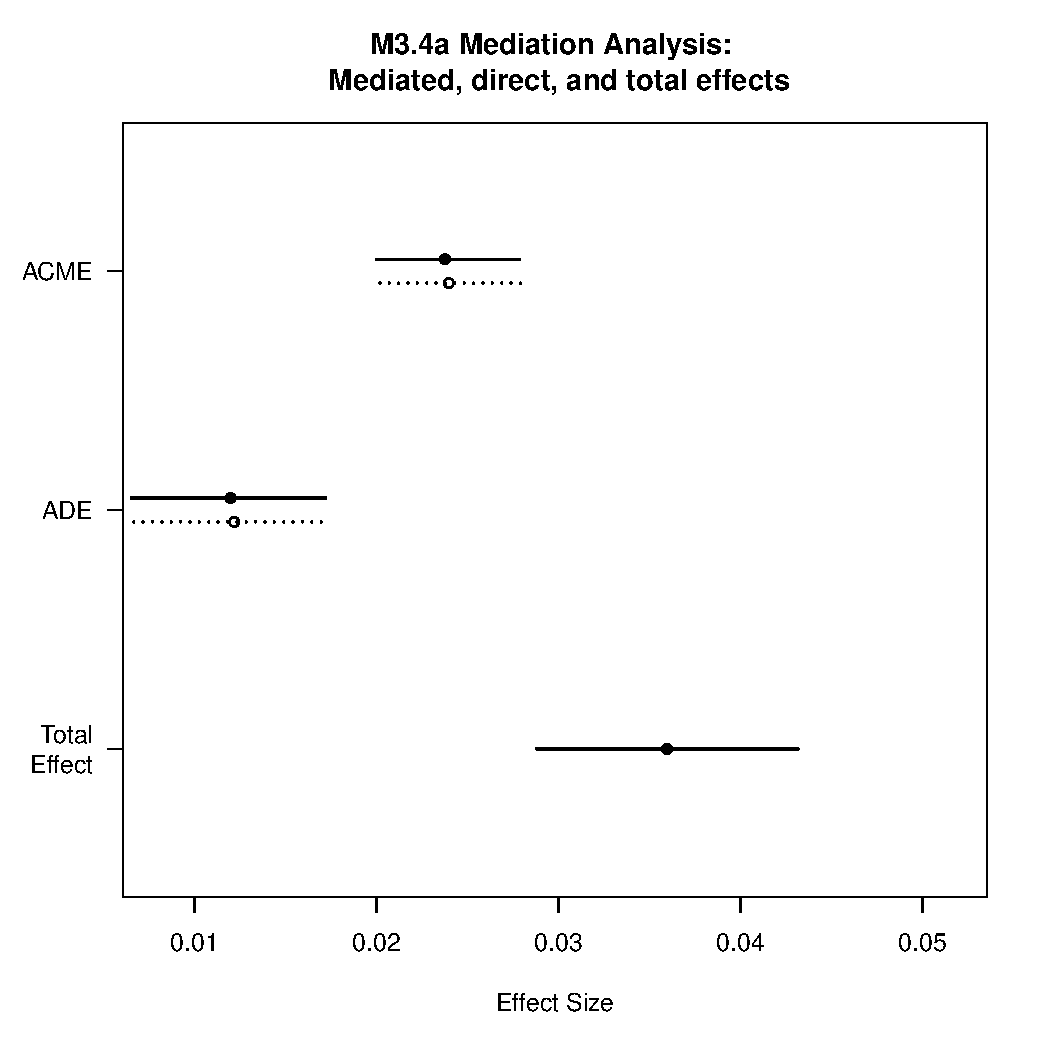
\includegraphics[width =\columnwidth]{images/MLM34aMediationAnalysis.pdf}
  \caption{M3.4a Mediation Analysis}
  \label{fig:MLM34aMediationAnalysis}
\end{figure}


\subsubsection{Discussion of overall Tournament results}





  \section{Discussion of Results}

  The results presented above generally support the central hypothesis of this dissertation, namely that relationship the relationship between joint action and social bonding is mediated by the feeling of ``team click.''  Results of analyses concerning both the post-Tournament survey and change between and pre- and post -Tournament surveys display a clear relationship between perceptions of Joint Action Success and Team Click, Team Click and Social Bonding, and a direct relationship between Joint Action Success and Social Bonding.  In the post-Tournament analysis, Team Click fully mediates the relationship between Joint Action Success and Social Bonding. In the pre-post analysis, Team Click partially mediates this relationship (this statistic was not significant, but was trending in the predicted direction, $p = .06$).

  Results of models designed to test the predicted relationships between Team Performance Expectations, Team Click, and Social Bonding also provided support for some but not all predictions. A relationship was confirmed between team performance expectation violation and team click, but not between expectation violation and social bonding. In addition, the predicted interaction between Joint Action Success, Team Performance Expectations, and Team Click was not significant, nor was the interaction between these same two predictor variables and social bonding.  Team click did not mediate the predicted relationship between violations of expectations around team performance and social bonding. The model of this direct relationship was not statistically robust using the data collected in this study.

  These results suggests that while expectation violation in joint action might be an important factor in generating feelings of team click, it might not be a strong enough mechanism to drive social bonding directly.  In contrast to the single-item measure of Team Performance Expectations, Joint Action Success is a factor made up of four items that require detailed reflection on the experience of four different aspects of team coordination.  This item may have more powerfully tapped into the implicit mechanisms involved in coordinated joint action, encouraging athletes to reflect on coordination with specific co-actors, and as such the opportunity to rehearse and reinforce feelings of trust, reliability, and cooperation \citep{Reddish2013a}.  It is also possible that expectation violation in joint action might not be immediately available to athlete reflection.
  As Frith and colleagues point out \textcite{Frith2007,Frith2010,Clark2013}, the generation of interoceptive predictive models for action implicates cognitive processes that exist largely below the surface of conscious awareness, and the relationship between these unconscious informational transfer in movement coordination and the small fraction of information that does make its way to consciousness in the form of higher order symbolic and linguistic representations is still not clearly understood \citep{Semin2008}. Team click might be supported by various subtle, implicit, and pre-perceptual processes involved in ``active inference'' \citep{Schmidt2011}.

  Evidence presented here does however support the interpretations that perceptions of joint action success predict social bonding, mediated by the experience of ``team click.'' It was predicted that technical competence may condition the relationship between perceptions of joint action, team click, and social bonding, owing to the possibility that more expert athletes could be more likely experience less pronounced discrepancy between expected and actual performance \cite{Tomeo2012}.  In this specific study, there was no evidence that technical competence---objective competence (training age, years in team, age) and self-reported competence (ability versus teammates, Chinese opponents, or international professionals)---significantly influenced variables of interest.  It is possible, as noted above, that these measures failed to access the (largely pre-perceptual) mechanisms of prediction error management hypothesised to underpin cognition and affective dispositions in joint action.  It is also possible that the nature of the intensity and consequentiality of the Tournament in which athletes were participating was high enough that no one---experts athletes included---was immune to the uncertainty and stress of this experience. Indeed, the ability of competitive group exercise contests to consistently arouse high levels of psychological stress and uncertainty could be an important reason for their cultural evolutionary success over recent centuries.

  In addition to technical competence of individual athletes, preexisting dispositional tendencies in dimensions of personality (e.g., extroversion, agreeableness) and physical endowment could impact on processes of social bonding \citep{Marsh2009,VonRueden2015}.   It has been documented that personality types correspond with basal tendencies for movement and movement coordination. In a joint action task involving two people of different heights moving wooden planks of different lengths, for example, Richardson and colleagues \textcite{Richardson2007} found that individuals’ levels of agreeableness and extroversion were positively correlated with the level of persistence of cooperation (hyteresis).  In particular, in the condition in which wooden planks increased in length (therefore increasing in demand for cooperative action), the degree of cooperation was positively correlated with the taller of the pair’s extroversion; the degree of cooperation in the random condition (where planks were received in no ordinal sequence of sizing) was correlated with the agreeableness of the shorter (i.e., more constraining) of the individuals.  I used the personality data collected in the pre-Tournament survey to test the relationship between personality types and team click. Interestingly, none of the big five personality types (extraversion, agreeableness, openness, conscientiousness, and neuroticism) significantly predicted feelings of team click in the post-Tournament survey.

  The impact of inter-individual psychophysiological variation on joint action can also be seen in the case of social dysfunctions such as autism spectrum disorder \citep{Isenhower2012} and schizophrenia \citep{Varlet2012}.  Generally speaking,  while autism spectrum disorder appears to be associated with deficits in anticipatory timing adjustments in intra- and inter-individual coordination of physical movement \citep{Martineau2010}, schizophrenia appears linked to a lack of prediction error management, due to failure in the neurological mechanisms through which predictions about the consequences of an action are derived \citep{Frith2000}.  Delusions of control owing to misattribution of agency are well-documented in schizophrenic patients---either delusions of self-control over external actions and events, or, alternatively, delusions involving the control of others over the individual (in the case of split personality and associated hallucinations) \citep{Frith2007}. It is quite possible that the experience of ``team click'' is an analogue, albeit much socially functional, to the pathological over-activity of agency-attribution mechanisms observed in schizophrenic patients.  The question of individual variation in sociability and movement tendencies should be further assessed in future studies.

  The fact that the hypothesised mechanisms of joint action and social bonding have been shown to exist pre-declaratively and predominantly below the surface of conscious experience presents a methodological challenge for psychological research which relies heavily on self-report.  Further exploring the relationship between pre-perceptual regulatory mechanisms of joint action and their psychosocial effects will require the use of other methods of data collection and analysis in order to triangulate the reliability of self-report data \citep{Newell2014}.  In this specific example, video footage showing athlete performance and coordination could be assessed using already established methods of motion capture and analysis to provide pseudo-objective measures of interpersonal and team-level synchrony in joint action \citep[e.g.][]{Passos2011}.
  Importantly, video footage analysis allows for the testing between different proposed mechanisms associated with joint action and social bonding,  For example, motion capture from video footage allows for measuring synchrony between co-actors could using both traditional methods of dimension reduction and principal component analysis \citep[see for example][]{Riley2011} as well as emerging methods borrowed from dynamic systems theory including fractal-like 1/f scaling (``pink noise'') \citep[see for example][]{Holden2013}. It is quite possible that these different measurements of synchrony could access different psychophysiological dimensions of the relationship between joint action and social bonding.  Other physiological markers of social interaction such as heart rate variability \citep{Konvalinka2011,Fischer2014a} and pain threshold \citep{Cohen2009,Tarr2015}) are beginning to be developed and tested in both experimental and real-world settings.
  These novel methodological approaches help complement existing behavioural measures, such as such as economic games \citep{Xygalatas2013} and spontaneous helping tasks \citep{Kirschner2010}, designed to access psychological mechanisms related to social bonding and cooperation.
  Together, these measures could then be compared to self-report measures derived from athlete self-report to more fully understand the ways in which component mechanisms and system dynamics of joint action generate social cohesion \citep{Marsh2009}.

  In sum, the results reported in this study provide novel evidence that feelings of team click mediate a relationship between perceived joint action success and social bonding, substantiating the claim that under certain circumstances joint action and interpersonal coordination processes can generate feelings of social connection \citep{Marsh2009}. Relationships between expectation violation, team click, and social bonding
  also confirmed, but these models are less robust, and should be treated with caution. All reported results hold when statistically controlling for measures relating to individual performance, objective competence, and actual Tournament performance outcomes in the Tournament, including Tournament rank, points scored, minutes played, and so on.  Of course, the uncontrolled and \textit{in-situ} design of this study means that results are correlational, and as such the predictions of this dissertation, only partially confirmed in this study, require further attention via a controlled experimental design.  An experiment in which joint action success and expectation violation were manipulated, and explicit feedback around performance was eliminated, could allow for the assessment of the role of the cognitive processes of movement coordination in joint action in generating team click and social bonding.  In addition, a controlled experiment offers the opportunity to utilise other measurements of synchrony, such as those derived from motion capture from video recordings.





%    [ ] what inferences can we make from these results?
%    [ ] How does it relate to other literature?
%    [ ] limitations
%    [ ] future work —> experiment (takes away explicit feedback)
%    [ ]  "Conclude the general discussion with a strong paragraph stating the main point or points again, in somewhat different terms-if possible-than used before.”

%\include{text/6trainingExperiment}
%\chapter{\label{generalDiscussion}General Discussion}

\textit{[Not included for CoS assessment]} \\
A general discussion will follow the analysis of the Ethnographic evidence and  training Tournament. The discussion will make theoretical inferences based on an assessment of results of all three studies.  Limitations of this study will be outlined, and future directions for research will be suggested.

\section{Timeline for Completion}
I propose the following timeline for completion:

\begin{description}
  \item [September:] Preparation for CoS Viva, Analyse training experiment
  \item [October:] Analyse training experiment and prepare report
  \item [November:] Analyse ethnographic data
  \item [December:] Prepare ethnographic data report
  \item [January:] Prepare general discussion
  \item [February:] Compose introduction, conclusion
  \item [March:] Refine
  \item [April:]
  \item [May:]
  \item [June:] Submit Final Thesis
\end{description}

%\chapter{\label{conclusion}Conclusion}

\textit{[Not included for CoS assessment]} \\
A general conclusion to will summarise the results and implications of this dissertation for cognitive and evolutionary anthropology.



%% APPENDICES %%
% Starts lettered appendices, adds a heading in table of contents, and adds a
%    page that just says "Appendices" to signal the end of your main text.
%\startappendices
% Add or remove any appendices you'd like here:
%\include{text/appendix}


%%%%% REFERENCES

% JEM: Quote for the top of references (just like a chapter quote if you're using them).  Comment to skip.
%\begin{savequote}[8cm]
%The first kind of intellectual and artistic personality belongs to the hedgehogs, the second to the foxes \dots
%  \qauthor{--- Sir Isaiah Berlin \cite{berlin_hedgehog_2013}}
%\end{savequote}

\setlength{\baselineskip}{0pt} % JEM: Single-space References

{\renewcommand*\MakeUppercase[1]{#1}%
\printbibliography[heading=bibintoc,title={\bibtitle}]}


\end{document}
